% Run LaTeX on this file several times to get Table of Contents,
%% cross-references, and citations.

\documentclass[11pt]{book}
\usepackage{gvv-book}
\usepackage{gvv} 
\usepackage{vaman-esp32/arduino-uart/figs/circuit}       
%\usepackage{Wiley-AuthoringTemplate}
\usepackage[sectionbib,authoryear]{natbib}% for name-date citation comment the below line
%\usepackage[sectionbib,numbers]{natbib}% for numbered citation comment the above line

%%********************************************************************%%
%%       How many levels of section head would you like numbered?     %%
%% 0= no section numbers, 1= section, 2= subsection, 3= subsubsection %%
\setcounter{secnumdepth}{3}
%%********************************************************************%%
%%**********************************************************************%%
%%     How many levels of section head would you like to appear in the  %%
%%				Table of Contents?			%%
%% 0= chapter, 1= section, 2= subsection, 3= subsubsection titles.	%%
\setcounter{tocdepth}{2}
%%**********************************************************************%%

%\includeonly{ch01}
\makeindex
\begin{document}

\frontmatter
%%%%%%%%%%%%%%%%%%%%%%%%%%%%%%%%%%%%%%%%%%%%%%%%%%%%%%%%%%%%%%%%
%% Title Pages
%% Wiley will provide title and copyright page, but you can make
%% your own titlepages if you'd like anyway
%% Setting up title pages, type in the appropriate names here:

\booktitle{Embedded System}

%\subtitle{Through Embedded Programming}

\AuAff{G. V. V. Sharma}


%% \\ will start a new line.
%% You may add \affil{} for affiliation, ie,
%\authors{Robert M. Groves\\
%\affil{Universitat de les Illes Balears}
%Floyd J. Fowler, Jr.\\
%\affil{University of New Mexico}
%}

%% Print Half Title and Title Page:
%\halftitlepage
\titlepage

%%%%%%%%%%%%%%%%%%%%%%%%%%%%%%%%%%%%%%%%%%%%%%%%%%%%%%%%%%%%%%%%
%% Copyright Page

\begin{copyrightpage}{2023}
%Title, etc
\end{copyrightpage}

% Note, you must use \ to start indented lines, ie,
% 
% \begin{copyrightpage}{2004}
% Survey Methodology / Robert M. Groves . . . [et al.].
% \       p. cm.---(Wiley series in survey methodology)
% \    ``Wiley-Interscience."
% \    Includes bibliographical references and index.
% \    ISBN 0-471-48348-6 (pbk.)
% \    1. Surveys---Methodology.  2. Social 
% \  sciences---Research---Statistical methods.  I. Groves, Robert M.  II. %
% Series.\\

% HA31.2.S873 2004
% 001.4'33---dc22                                             2004044064
% \end{copyrightpage}

%%%%%%%%%%%%%%%%%%%%%%%%%%%%%%%%%%%%%%%%%%%%%%%%%%%%%%%%%%%%%%%%
%% Only Dedication (optional) 

%\dedication{To my parents}

\tableofcontents

%\listoffigures %optional
%\listoftables  %optional

%% or Contributor Page for edited books
%% before \tableofcontents

%%%%%%%%%%%%%%%%%%%%%%%%%%%%%%%%%%%%%%%%%%%%%%%%%%%%%%%%%%%%%%%%
%  Contributors Page for Edited Book
%%%%%%%%%%%%%%%%%%%%%%%%%%%%%%%%%%%%%%%%%%%%%%%%%%%%%%%%%%%%%%%%

% If your book has chapters written by different authors,
% you'll need a Contributors page.

% Use \begin{contributors}...\end{contributors} and
% then enter each author with the \name{} command, followed
% by the affiliation information.

% \begin{contributors}
% \name{Masayki Abe,} Fujitsu Laboratories Ltd., Fujitsu Limited, Atsugi, Japan
%
% \name{L. A. Akers,} Center for Solid State Electronics Research, Arizona State University, Tempe, Arizona
%
% \name{G. H. Bernstein,} Department of Electrical and Computer Engineering, University of Notre Dame, Notre Dame, South Bend, Indiana; formerly of
% Center for Solid State Electronics Research, Arizona
% State University, Tempe, Arizona 
% \end{contributors}

%%%%%%%%%%%%%%%%%%%%%%%%%%%%%%%%%%%%%%%%%%%%%%%%%%%%%%%%%%%%%%%%
% Optional Foreword:

%\begin{foreword}
%\lipsum[1-2]
%\end{foreword}

%%%%%%%%%%%%%%%%%%%%%%%%%%%%%%%%%%%%%%%%%%%%%%%%%%%%%%%%%%%%%%%%
% Optional Preface:

%\begin{preface}
%\lipsum[1-1]
%\prefaceauthor{}
%\where{place\\
% date}
%\end{preface}

% ie,
% \begin{preface}
% This is an example preface.
% \prefaceauthor{R. K. Watts}
% \where{Durham, North Carolina\\
% September, 2004}

%%%%%%%%%%%%%%%%%%%%%%%%%%%%%%%%%%%%%%%%%%%%%%%%%%%%%%%%%%%%%%%%
% Optional Acknowledgments:

%\acknowledgments
%\lipsum[1-2]
%\authorinitials{I. R. S.}  

%%%%%%%%%%%%%%%%%%%%%%%%%%%%%%%%
%% Glossary Type of Environment:

% \begin{glossary}
% \term{<term>}{<description>}
% \end{glossary}

%%%%%%%%%%%%%%%%%%%%%%%%%%%%%%%%
%\begin{acronyms}
%\acro{ASTA}{Arrivals See Time Averages}
%\acro{BHCA}{Busy Hour Call Attempts}
%\acro{BR}{Bandwidth Reservation}
%\acro{b.u.}{bandwidth unit(s)}
%\acro{CAC}{Call / Connection Admission Control}
%\acro{CBP}{Call Blocking Probability(-ies)}
%\acro{CCS}{Centum Call Seconds}
%\acro{CDTM}{Connection Dependent Threshold Model}
%\acro{CS}{Complete Sharing}
%\acro{DiffServ}{Differentiated Services}
%\acro{EMLM}{Erlang Multirate Loss Model}
%\acro{erl}{The Erlang unit of traffic-load}
%\acro{FIFO}{First in - First out}
%\acro{GB}{Global balance}
%\acro{GoS}{Grade of Service}
%\acro{ICT}{Information and Communication Technology}
%\acro{IntServ}{Integrated Services}
%\acro{IP}{Internet Protocol}
%\acro{ITU-T}{International Telecommunication Unit -- Standardization sector}
%\acro{LB}{Local balance}
%\acro{LHS}{Left hand side}
%\acro{LIFO}{Last in - First out}
%\acro{MMPP}{Markov Modulated Poisson Process}
%\acro{MPLS}{Multiple Protocol Labeling Switching}
%\acro{MRM}{Multi-Retry Model}
%\acro{MTM}{Multi-Threshold Model}
%\acro{PASTA}{Poisson Arrivals See Time Averages}
%\acro{PDF}{Probability Distribution Function}
%\acro{pdf}{probability density function}
%\acro{PFS}{Product Form Solution}
%\acro{QoS}{Quality of Service}
%\acro{r.v.}{random variable(s)}
%\acro{RED}{random early detection}
%\acro{RHS}{Right hand side}
%\acro{RLA}{Reduced Load Approximation}
%\acro{SIRO}{service in random order}
%\acro{SRM}{Single-Retry Model}
%\acro{STM}{Single-Threshold Model}
%\acro{TCP}{Transport Control Protocol}
%\acro{TH}{Threshold(s)}
%\acro{UDP}{User Datagram Protocol}
%\end{acronyms}

\setcounter{page}{1}

\begin{introduction}
This book introduces Embedded Systems through using the Vaman framework.
\end{introduction}

\mainmatter
\chapter{Vaman-ESP32}
This chapter contains various experiments that can be performed using the 
Vaman-ESP32.
\section{Flash Vaman-ESP32 Using Arduino}
\renewcommand{\theequation}{\theenumi}
\renewcommand{\thefigure}{\theenumi}
\begin{enumerate}[label=\thesection.\arabic*.,ref=\thesection.\theenumi]
\numberwithin{equation}{enumi}
\numberwithin{figure}{enumi}
\numberwithin{table}{enumi}
\item Make sure that Vaman board do not power any devices.  
\item Make connections as shown in \tabref{tab:arduino-uart} and  \figref{fig:vaman/uart/1}. 
\item The Vaman pin diagram is available in \figref{fig:vaman-pin_sheet}
\begin{figure}[!ht]
\centering
\begin{tikzpicture}
         
         \draw             
             (2,4) node[arduino] (arduino1) {}
             (15,4) node[Vaman] (test){}
             (arduino1.Rx) to (5,7) to [R] (7,7) to [R](9.5,7) to [R](11.5,7)
             (11.5,7) node[ground]{}  
             (7,7) to (7,8) to (12,8) to (12,7) to (test.Rx)
             (arduino1.Tx) to (5,6) to [R] (7,6) to [R](9.5,6) to [R](11.5,6)
             (11.5,6) node[ground]{}  
             (7,6) to (7,5) to (12,5) to (12,6) to (test.Tx)
             %(arduno1.D13) to(6,7) to [R](6,3) to [leDo](6,-0.9)             
             (arduino1.GND) to(test.GND)
             (arduino1.3V) to (test.3V)
             (arduino1.RST) node[ground]{}
             (12.6,3) to (12.6,2.5) node[ground]{}
         ;
         
         \node[align=left] at (6,7.5) {1K $\Omega$};
         \node[align=left] at (6,6.5) {1K $\Omega$};
         \node[align=left] at (8.5,6.5) {1K $\Omega$};
         \node[align=left] at (8.5,7.5) {1K $\Omega$};
         \node[align=left] at (10.5,6.5) {1K $\Omega$};
         \node[align=left] at (10.5,7.5) {1K $\Omega$};
             
    \end{tikzpicture}


\caption{Circuit Connections}
\label{fig:vaman/uart/1}
\end{figure}
\begin{figure}
\centering
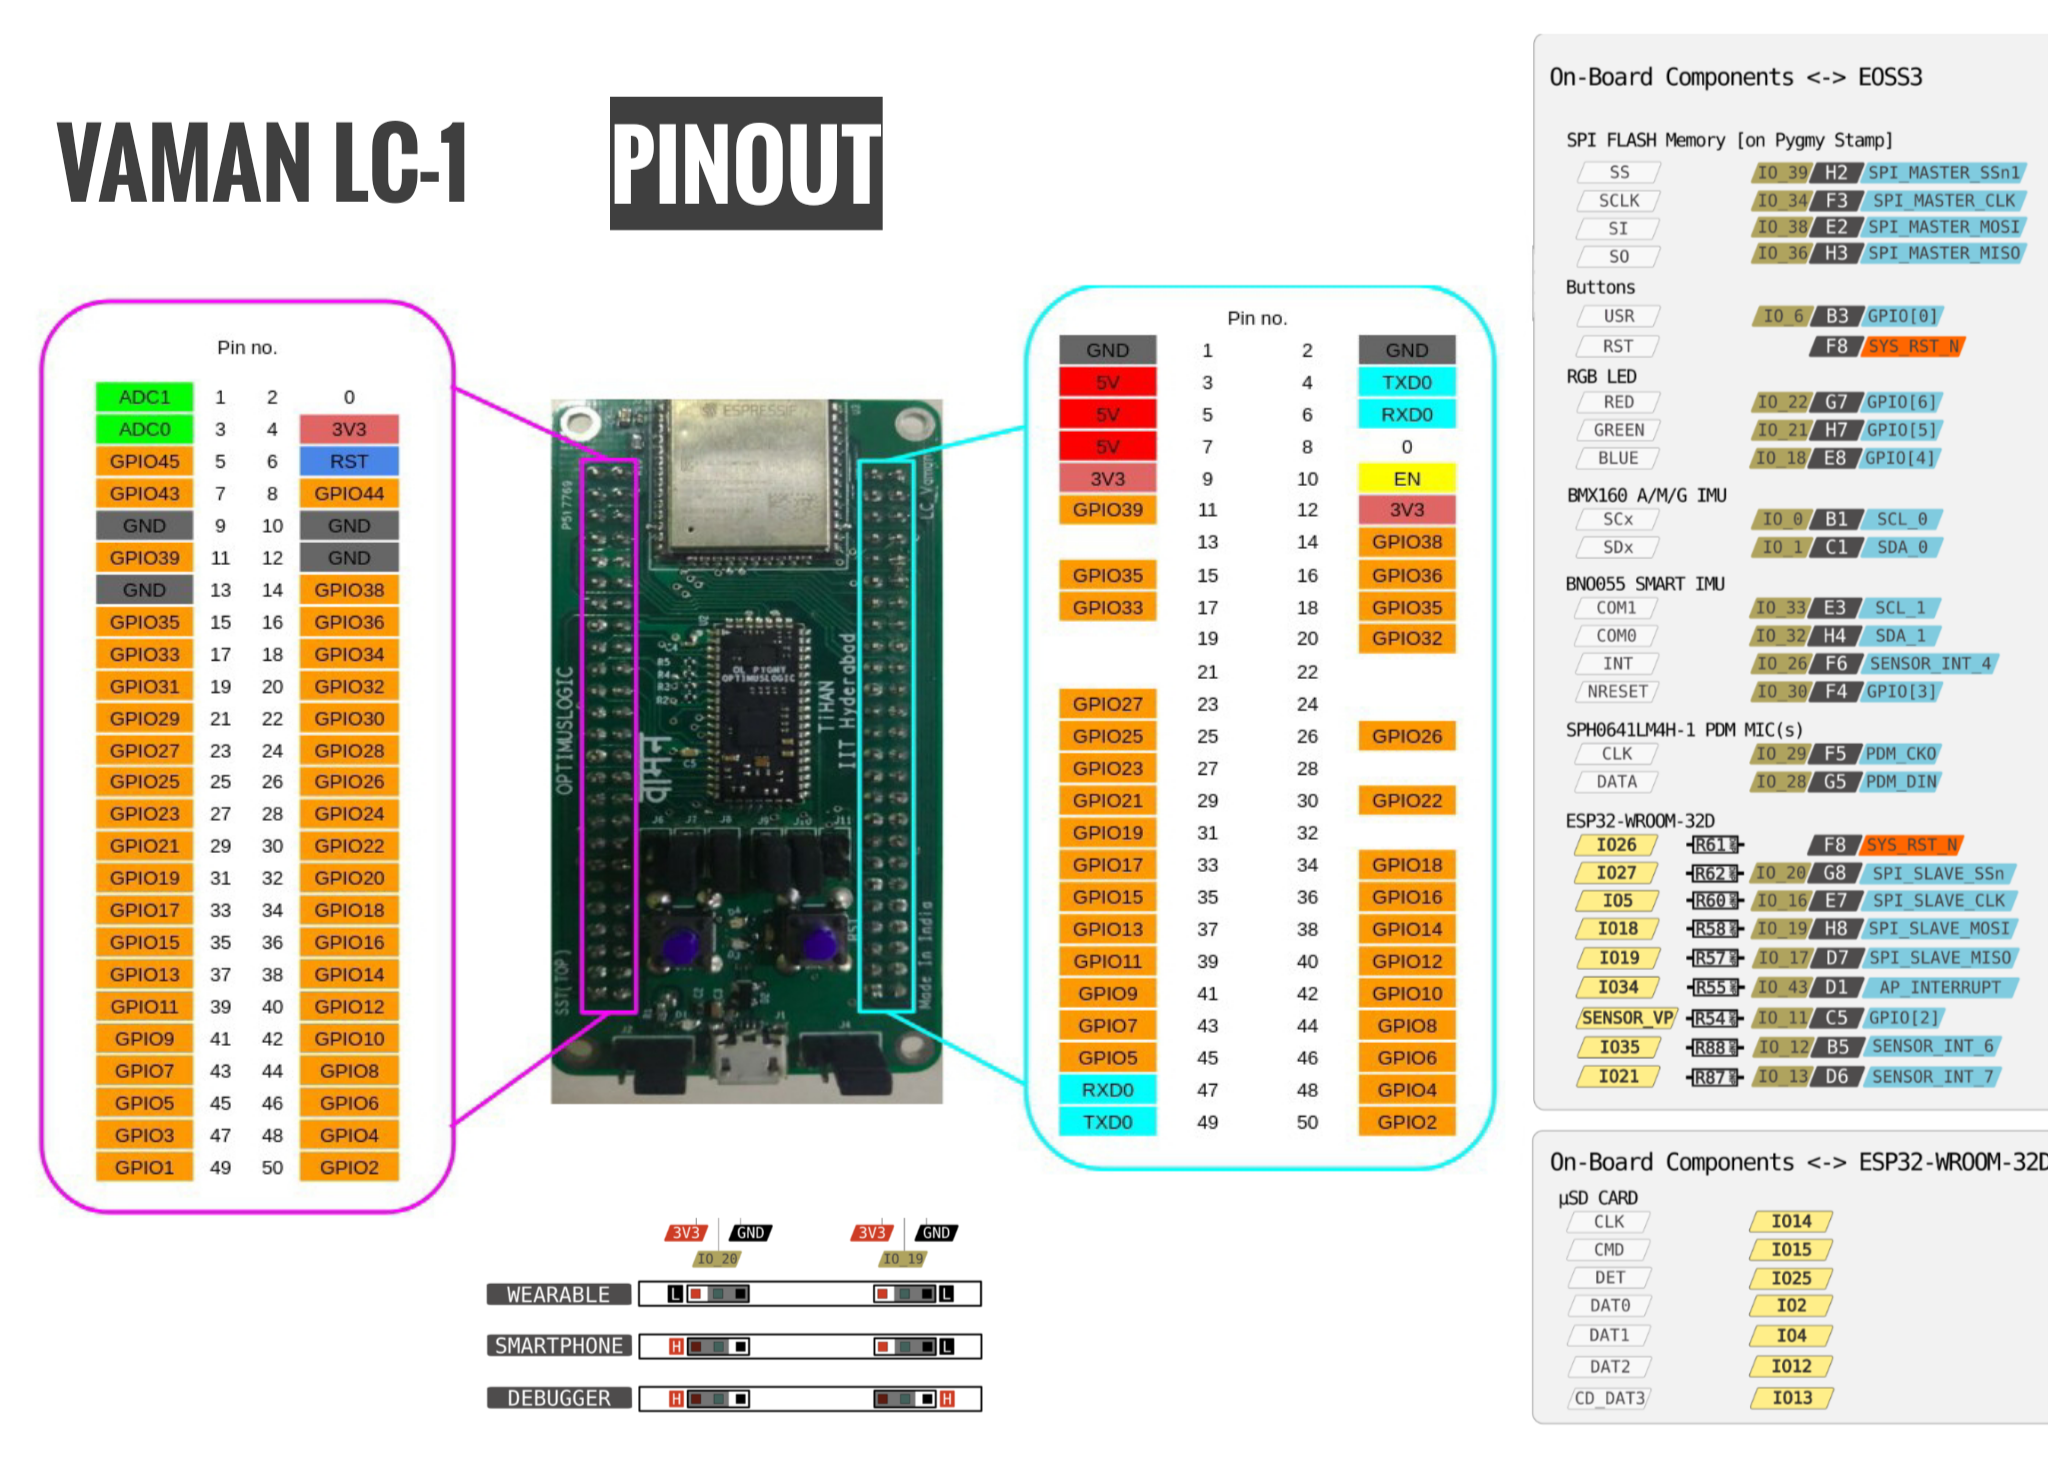
\includegraphics[width=\columnwidth]{vaman-esp32/lcd/figs/pin_sheet.png}
\caption{Vaman pins}
\label{fig:vaman-pin_sheet}
\end{figure}
\begin{table}[!ht]
%%%%%%%%%%%%%%%%%%%%%%%%%%%%%%%%%%%%%%%%%%%%%%%%%%%%%%%%%%%%%%%%%%%%%%
%%                                                                  %%
%%  This is the header of a LaTeX2e file exported from Gnumeric.    %%
%%                                                                  %%
%%  This file can be compiled as it stands or included in another   %%
%%  LaTeX document. The table is based on the longtable package so  %%
%%  the longtable options (headers, footers...) can be set in the   %%
%%  preamble section below (see PRAMBLE).                           %%
%%                                                                  %%
%%  To include the file in another, the following two lines must be %%
%%  in the including file:                                          %%
%%        \def\inputGnumericTable{}                                 %%
%%  at the beginning of the file and:                               %%
%%        \input{name-of-this-file.tex}                             %%
%%  where the table is to be placed. Note also that the including   %%
%%  file must use the following packages for the table to be        %%
%%  rendered correctly:                                             %%
%%    \usepackage[latin1]{inputenc}                                 %%
%%    \usepackage{color}                                            %%
%%    \usepackage{array}                                            %%
%%    \usepackage{longtable}                                        %%
%%    \usepackage{calc}                                             %%
%%    \usepackage{multirow}                                         %%
%%    \usepackage{hhline}                                           %%
%%    \usepackage{ifthen}                                           %%
%%  optionally (for landscape tables embedded in another document): %%
%%    \usepackage{lscape}                                           %%
%%                                                                  %%
%%%%%%%%%%%%%%%%%%%%%%%%%%%%%%%%%%%%%%%%%%%%%%%%%%%%%%%%%%%%%%%%%%%%%%



%%  This section checks if we are begin input into another file or  %%
%%  the file will be compiled alone. First use a macro taken from   %%
%%  the TeXbook ex 7.7 (suggestion of Han-Wen Nienhuys).            %%
\def\ifundefined#1{\expandafter\ifx\csname#1\endcsname\relax}


%%  Check for the \def token for inputed files. If it is not        %%
%%  defined, the file will be processed as a standalone and the     %%
%%  preamble will be used.                                          %%
\ifundefined{inputGnumericTable}

%%  We must be able to close or not the document at the end.        %%
	\def\gnumericTableEnd{\end{document}}


%%%%%%%%%%%%%%%%%%%%%%%%%%%%%%%%%%%%%%%%%%%%%%%%%%%%%%%%%%%%%%%%%%%%%%
%%                                                                  %%
%%  This is the PREAMBLE. Change these values to get the right      %%
%%  paper size and other niceties.                                  %%
%%                                                                  %%
%%%%%%%%%%%%%%%%%%%%%%%%%%%%%%%%%%%%%%%%%%%%%%%%%%%%%%%%%%%%%%%%%%%%%%

	\documentclass[12pt%
			  %,landscape%
                    ]{report}
       \usepackage[latin1]{inputenc}
       \usepackage{fullpage}
       \usepackage{color}
       \usepackage{array}
       \usepackage{longtable}
       \usepackage{calc}
       \usepackage{multirow}
       \usepackage{hhline}
       \usepackage{ifthen}

	\begin{document}


%%  End of the preamble for the standalone. The next section is for %%
%%  documents which are included into other LaTeX2e files.          %%
\else

%%  We are not a stand alone document. For a regular table, we will %%
%%  have no preamble and only define the closing to mean nothing.   %%
    \def\gnumericTableEnd{}

%%  If we want landscape mode in an embedded document, comment out  %%
%%  the line above and uncomment the two below. The table will      %%
%%  begin on a new page and run in landscape mode.                  %%
%       \def\gnumericTableEnd{\end{landscape}}
%       \begin{landscape}


%%  End of the else clause for this file being \input.              %%
\fi

%%%%%%%%%%%%%%%%%%%%%%%%%%%%%%%%%%%%%%%%%%%%%%%%%%%%%%%%%%%%%%%%%%%%%%
%%                                                                  %%
%%  The rest is the gnumeric table, except for the closing          %%
%%  statement. Changes below will alter the table's appearance.     %%
%%                                                                  %%
%%%%%%%%%%%%%%%%%%%%%%%%%%%%%%%%%%%%%%%%%%%%%%%%%%%%%%%%%%%%%%%%%%%%%%

\providecommand{\gnumericmathit}[1]{#1} 
%%  Uncomment the next line if you would like your numbers to be in %%
%%  italics if they are italizised in the gnumeric table.           %%
%\renewcommand{\gnumericmathit}[1]{\mathit{#1}}
\providecommand{\gnumericPB}[1]%
{\let\gnumericTemp=\\#1\let\\=\gnumericTemp\hspace{0pt}}
 \ifundefined{gnumericTableWidthDefined}
        \newlength{\gnumericTableWidth}
        \newlength{\gnumericTableWidthComplete}
        \newlength{\gnumericMultiRowLength}
        \global\def\gnumericTableWidthDefined{}
 \fi
%% The following setting protects this code from babel shorthands.  %%
 \ifthenelse{\isundefined{\languageshorthands}}{}{\languageshorthands{english}}
%%  The default table format retains the relative column widths of  %%
%%  gnumeric. They can easily be changed to c, r or l. In that case %%
%%  you may want to comment out the next line and uncomment the one %%
%%  thereafter                                                      %%
\providecommand\gnumbox{\makebox[0pt]}
%%\providecommand\gnumbox[1][]{\makebox}

%% to adjust positions in multirow situations                       %%
\setlength{\bigstrutjot}{\jot}
\setlength{\extrarowheight}{\doublerulesep}

%%  The \setlongtables command keeps column widths the same across  %%
%%  pages. Simply comment out next line for varying column widths.  %%
\setlongtables

\setlength\gnumericTableWidth{%
	98pt+%
	118pt+%
0pt}
\def\gumericNumCols{2}
\setlength\gnumericTableWidthComplete{\gnumericTableWidth+%
         \tabcolsep*\gumericNumCols*2+\arrayrulewidth*\gumericNumCols}
\ifthenelse{\lengthtest{\gnumericTableWidthComplete > \linewidth}}%
         {\def\gnumericScale{1*\ratio{\linewidth-%
                        \tabcolsep*\gumericNumCols*2-%
                        \arrayrulewidth*\gumericNumCols}%
{\gnumericTableWidth}}}%
{\def\gnumericScale{1}}

%%%%%%%%%%%%%%%%%%%%%%%%%%%%%%%%%%%%%%%%%%%%%%%%%%%%%%%%%%%%%%%%%%%%%%
%%                                                                  %%
%% The following are the widths of the various columns. We are      %%
%% defining them here because then they are easier to change.       %%
%% Depending on the cell formats we may use them more than once.    %%
%%                                                                  %%
%%%%%%%%%%%%%%%%%%%%%%%%%%%%%%%%%%%%%%%%%%%%%%%%%%%%%%%%%%%%%%%%%%%%%%

\ifthenelse{\isundefined{\gnumericColA}}{\newlength{\gnumericColA}}{}\settowidth{\gnumericColA}{\begin{tabular}{@{}p{98pt*\gnumericScale}@{}}x\end{tabular}}
\ifthenelse{\isundefined{\gnumericColB}}{\newlength{\gnumericColB}}{}\settowidth{\gnumericColB}{\begin{tabular}{@{}p{118pt*\gnumericScale}@{}}x\end{tabular}}

\begin{tabular}[c]{%
	b{\gnumericColA}%
	b{\gnumericColB}%
	}

%%%%%%%%%%%%%%%%%%%%%%%%%%%%%%%%%%%%%%%%%%%%%%%%%%%%%%%%%%%%%%%%%%%%%%
%%  The tabular options. (Caption, headers... see Goosens, p.124) %%
%	\caption{The Table Caption.}             \\	%
% \hline	% Across the top of the table.
%%  The rest of these options are table rows which are placed on    %%
%%  the first, last or every page. Use \multicolumn if you want.    %%

%%  Header for the first page.                                      %%
%	\multicolumn{2}{c}{The First Header} \\ \hline 
%	\multicolumn{1}{c}{colTag}	%Column 1
%	&\multicolumn{1}{c}{colTag}	\\ \hline %Last column
%	\endfirsthead

%%  The running header definition.                                  %%
%	\hline
%	\multicolumn{2}{l}{\ldots\small\slshape continued} \\ \hline
%	\multicolumn{1}{c}{colTag}	%Column 1
%	&\multicolumn{1}{c}{colTag}	\\ \hline %Last column
%	\endhead

%%  The running footer definition.                                  %%
%	\hline
%	\multicolumn{2}{r}{\small\slshape continued\ldots} \\
%	\endfoot

%%  The ending footer definition.                                   %%
%	\multicolumn{2}{c}{That's all folks} \\ \hline 
%	\endlastfoot
%%%%%%%%%%%%%%%%%%%%%%%%%%%%%%%%%%%%%%%%%%%%%%%%%%%%%%%%%%%%%%%%%%%%%%

\hhline{|-|-}
	 \multicolumn{1}{|p{\gnumericColA}|}%
	{\gnumericPB{\centering}\gnumbox{{\color[rgb]{0.79,0.13,0.12} VAMAN LC PINS}}}
	&\multicolumn{1}{p{\gnumericColB}|}%
	{\gnumericPB{\centering}\gnumbox{{\color[rgb]{0.79,0.13,0.12} ARDUINO PINS}}}
\\
\hhline{|--|}
	 \multicolumn{1}{|p{\gnumericColA}|}%
	{\gnumericPB{\centering}\gnumbox{3.3}}
	&\multicolumn{1}{p{\gnumericColB}|}%
	{\gnumericPB{\centering}\gnumbox{3.3}}
\\
\hhline{|--|}
	 \multicolumn{1}{|p{\gnumericColA}|}%
	{\gnumericPB{\centering}\gnumbox{GND}}
	&\multicolumn{1}{p{\gnumericColB}|}%
	{\gnumericPB{\centering}\gnumbox{GND}}
\\
\hhline{|--|}
	 \multicolumn{1}{|p{\gnumericColA}|}%
	{\gnumericPB{\centering}\gnumbox{TXD0}}
	&\multicolumn{1}{p{\gnumericColB}|}%
	{\gnumericPB{\centering}\gnumbox{TXD}}
\\
\hhline{|--|}
	 \multicolumn{1}{|p{\gnumericColA}|}%
	{\gnumericPB{\centering}\gnumbox{RXD0}}
	&\multicolumn{1}{p{\gnumericColB}|}%
	{\gnumericPB{\centering}\gnumbox{RXD}}
\\
\hhline{|--|}
	 \multicolumn{1}{|p{\gnumericColA}|}%
	{\gnumericPB{\centering}\gnumbox{0}}
	&\multicolumn{1}{p{\gnumericColB}|}%
	{\gnumericPB{\centering}\gnumbox{GND}}
\\
\hhline{|--|}
	 \multicolumn{1}{|p{\gnumericColA}|}%
	{\gnumericPB{\centering}\gnumbox{EN}}
	&\multicolumn{1}{p{\gnumericColB}|}%
	{\gnumericPB{\centering}\gnumbox{GND}}
\\
\hhline{|-|-|}
\end{tabular}

\ifthenelse{\isundefined{\languageshorthands}}{}{\languageshorthands{\languagename}}
\gnumericTableEnd

\caption{}
\label{tab:arduino-uart}
\end{table}
\item For compiling and genrating the bin file 
\item make sure that platformio.ini file contains these lines
\begin{lstlisting}
[env:esp32doit-devkit-v1]
platform = espressif32
board = esp32doit-devkit-v1
framework = arduino
platform_packages =                                                               toolchain-xtensa-esp32@https://github.com/esphome/esphome-docker-base/releases/download/v1.4.0/toolchain-xtensa32.tar.gz                             
framework-arduinoespressif32@<3.10006.210326
\end{lstlisting}
\item For uploading bin file to Vaman through ArduinoDroid application 
\begin{lstlisting}[language=bash]
1. Open the Droid Application
2. Click the three dots in the top right corner
3. Navigate to Settings -> Board Type
4. Select ESP32 -> DOIT ESP32 DEVKIT V1
5. Change the upload speed to 115200
6. Upload the generated .bin file
\end{lstlisting}
\item While the dots are printed on the screen, disconnect the EN wire from GND.   Make sure that the Vaman board is not powering any device while flashing.  The Vaman-ESP should now flash.
\item After flashing, disconnect pin 0 on Vaman-ESP from GND. Power on Vaman appropriately.
\end{enumerate}

\section{Measuring Unknown Resistance}
This section describes how to measure an unknown resistance through Vaman-ESP32 
and display it on an LCD.
\subsection{Components}
\numberwithin{equation}{enumi}
\numberwithin{figure}{enumi}
\numberwithin{table}{section}

\begin{table}[!ht]
\centering
%%%%%%%%%%%%%%%%%%%%%%%%%%%%%%%%%%%%%%%%%%%%%%%%%%%%%%%%%%%%%%%%%%%%%%
%%                                                                  %%
%%  This is the header of a LaTeX2e file exported from Gnumeric.    %%
%%                                                                  %%
%%  This file can be compiled as it stands or included in another   %%
%%  LaTeX document. The table is based on the longtable package so  %%
%%  the longtable options (headers, footers...) can be set in the   %%
%%  preamble section below (see PRAMBLE).                           %%
%%                                                                  %%
%%  To include the file in another, the following two lines must be %%
%%  in the including file:                                          %%
%%        \def\inputGnumericTable{}                                 %%
%%  at the beginning of the file and:                               %%
%%        \input{name-of-this-file.tex}                             %%
%%  where the table is to be placed. Note also that the including   %%
%%  file must use the following packages for the table to be        %%
%%  rendered correctly:                                             %%
%%    \usepackage[latin1]{inputenc}                                 %%
%%    \usepackage{color}                                            %%
%%    \usepackage{array}                                            %%
%%    \usepackage{longtable}                                        %%
%%    \usepackage{calc}                                             %%
%%    \usepackage{multirow}                                         %%
%%    \usepackage{hhline}                                           %%
%%    \usepackage{ifthen}                                           %%
%%  optionally (for landscape tables embedded in another document): %%
%%    \usepackage{lscape}                                           %%
%%                                                                  %%
%%%%%%%%%%%%%%%%%%%%%%%%%%%%%%%%%%%%%%%%%%%%%%%%%%%%%%%%%%%%%%%%%%%%%%



%%  This section checks if we are begin input into another file or  %%
%%  the file will be compiled alone. First use a macro taken from   %%
%%  the TeXbook ex 7.7 (suggestion of Han-Wen Nienhuys).            %%
\def\ifundefined#1{\expandafter\ifx\csname#1\endcsname\relax}


%%  Check for the \def token for inputed files. If it is not        %%
%%  defined, the file will be processed as a standalone and the     %%
%%  preamble will be used.                                          %%
\ifundefined{inputGnumericTable}

%%  We must be able to close or not the document at the end.        %%
	\def\gnumericTableEnd{\end{document}}


%%%%%%%%%%%%%%%%%%%%%%%%%%%%%%%%%%%%%%%%%%%%%%%%%%%%%%%%%%%%%%%%%%%%%%
%%                                                                  %%
%%  This is the PREAMBLE. Change these values to get the right      %%
%%  paper size and other niceties.                                  %%
%%                                                                  %%
%%%%%%%%%%%%%%%%%%%%%%%%%%%%%%%%%%%%%%%%%%%%%%%%%%%%%%%%%%%%%%%%%%%%%%

	\documentclass[12pt%
			  %,landscape%
                    ]{report}
       \usepackage[latin1]{inputenc}
       \usepackage{fullpage}
       \usepackage{color}
       \usepackage{array}
       \usepackage{longtable}
       \usepackage{calc}
       \usepackage{multirow}
       \usepackage{hhline}
       \usepackage{ifthen}

	\begin{document}


%%  End of the preamble for the standalone. The next section is for %%
%%  documents which are included into other LaTeX2e files.          %%
\else

%%  We are not a stand alone document. For a regular table, we will %%
%%  have no preamble and only define the closing to mean nothing.   %%
    \def\gnumericTableEnd{}

%%  If we want landscape mode in an embedded document, comment out  %%
%%  the line above and uncomment the two below. The table will      %%
%%  begin on a new page and run in landscape mode.                  %%
%       \def\gnumericTableEnd{\end{landscape}}
%       \begin{landscape}


%%  End f the else clause for this file being \input.              %%
\fi

%%%%%%%%%%%%%%%%%%%%%%%%%%%%%%%%%%%%%%%%%%%%%%%%%%%%%%%%%%%%%%%%%%%%%%
%%                                                                  %%
%%  The rest is the gnumeric table, except for the closing          %%
%%  statement. Changes below will alter the table's appearance.     %%
%%                                                                  %%
%%%%%%%%%%%%%%%%%%%%%%%%%%%%%%%%%%%%%%%%%%%%%%%%%%%%%%%%%%%%%%%%%%%%%%

\providecommand{\gnumericmathit}[1]{#1} 
%%  Uncomment the next line if you would like your numbers to be in %%
%%  italics if they are italizised in the gnumeric table.           %%
%\renewcommand{\gnumericmathit}[1]{\mathit{#1}}
\providecommand{\gnumericPB}[1]%
{\let\gnumericTemp=\\#1\let\\=\gnumericTemp\hspace{0pt}}
 \ifundefined{gnumericTableWidthDefined}
        \newlength{\gnumericTableWidth}
        \newlength{\gnumericTableWidthComplete}
        \newlength{\gnumericMultiRowLength}
        \global\def\gnumericTableWidthDefined{}
 \fi
%% The following setting protects this code from babel shorthands.  %%
 \ifthenelse{\isundefined{\languageshorthands}}{}{\languageshorthands{english}}
%%  The default table format retains the relative column widths of  %%
%%  gnumeric. They can easily be changed to c, r or l. In that case %%
%%  you may want to comment out the next line and uncomment the one %%
%%  thereafter                                                      %%
\providecommand\gnumbox{\makebox[0pt]}
%%\providecommand\gnumbox[1][]{\makebox}

%% to adjust positions in multirow situations                       %%
\setlength{\bigstrutjot}{\jot}
\setlength{\extrarowheight}{\doublerulesep}

%%  The \setlongtables command keeps column widths the same across  %%
%%  pages. Simply comment out next line for varying column widths.  %%
\setlongtables

\setlength\gnumericTableWidth{%
	72pt+%
	52pt+%
	55pt+%
0pt}
\def\gumericNumCols{3}
\setlength\gnumericTableWidthComplete{\gnumericTableWidth+%
         \tabcolsep*\gumericNumCols*2+\arrayrulewidth*\gumericNumCols}
\ifthenelse{\lengthtest{\gnumericTableWidthComplete > \linewidth}}%
         {\def\gnumericScale{\ratio{\linewidth-%
                        \tabcolsep*\gumericNumCols*2-%
                        \arrayrulewidth*\gumericNumCols}%
{\gnumericTableWidth}}}%
{\def\gnumericScale{1}}

%%%%%%%%%%%%%%%%%%%%%%%%%%%%%%%%%%%%%%%%%%%%%%%%%%%%%%%%%%%%%%%%%%%%%%
%%                                                                  %%
%% The following are the widths of the various columns. We are      %%
%% defining them here because then they are easier to change.       %%
%% Depending on the cell formats we may use them more than once.    %%
%%                                                                  %%
%%%%%%%%%%%%%%%%%%%%%%%%%%%%%%%%%%%%%%%%%%%%%%%%%%%%%%%%%%%%%%%%%%%%%%

\ifthenelse{\isundefined{\gnumericColA}}{\newlength{\gnumericColA}}{}\settowidth{\gnumericColA}{\begin{tabular}{@{}p{72pt*\gnumericScale}@{}}x\end{tabular}}
\ifthenelse{\isundefined{\gnumericColB}}{\newlength{\gnumericColB}}{}\settowidth{\gnumericColB}{\begin{tabular}{@{}p{52pt*\gnumericScale}@{}}x\end{tabular}}
\ifthenelse{\isundefined{\gnumericColC}}{\newlength{\gnumericColC}}{}\settowidth{\gnumericColC}{\begin{tabular}{@{}p{55pt*\gnumericScale}@{}}x\end{tabular}}

\begin{tabular}[c]{%
	b{\gnumericColA}%
	b{\gnumericColB}%
	b{\gnumericColC}%
	}

%%%%%%%%%%%%%%%%%%%%%%%%%%%%%%%%%%%%%%%%%%%%%%%%%%%%%%%%%%%%%%%%%%%%%%
%%  The longtable options. (Caption, headers... see Goosens, p.124) %%
%	\caption{The Table Caption.}             \\	%
% \hline	% Across the top of the table.
%%  The rest of these options are table rows which are placed on    %%
%%  the first, last or every page. Use \multicolumn if you want.    %%

%%  Header for the first page.                                      %%
%	\multicolumn{3}{c}{The First Header} \\ \hline 
%	\multicolumn{1}{c}{colTag}	%Column 1
%	&\multicolumn{1}{c}{colTag}	%Column 2
%	&\multicolumn{1}{c}{colTag}	\\ \hline %Last column
%	\endfirsthead

%%  The running header definition.                                  %%
%	\hline
%	\multicolumn{3}{l}{\ldots\small\slshape continued} \\ \hline
%	\multicolumn{1}{c}{colTag}	%Column 1
%	&\multicolumn{1}{c}{colTag}	%Column 2
%	&\multicolumn{1}{c}{colTag}	\\ \hline %Last column
%	\endhead

%%  The running footer definition.                                  %%
%	\hline
%	\multicolumn{3}{r}{\small\slshape continued\ldots} \\
%	\endfoot

%%  The ending footer definition.                                   %%
%	\multicolumn{3}{c}{That's all folks} \\ \hline 
%	\endlastfoot
%%%%%%%%%%%%%%%%%%%%%%%%%%%%%%%%%%%%%%%%%%%%%%%%%%%%%%%%%%%%%%%%%%%%%%

\hhline{|-|-|-}
	 \multicolumn{1}{|p{\gnumericColA}|}%
	{\gnumericPB{\centering}\textbf{Component}}
	&\multicolumn{1}{p{\gnumericColB}|}%
	{\gnumericPB{\centering}\textbf{Value}}
	&\multicolumn{1}{p{\gnumericColC}|}%
	{\gnumericPB{\centering}\textbf{Quantity}}
\\
\hhline{|---|}
	 \multicolumn{1}{|p{\gnumericColA}|}%
	{\setlength{\gnumericMultiRowLength}{0pt}%
	 \addtolength{\gnumericMultiRowLength}{\gnumericColA}%
	 \multirow{2}[1]{\gnumericMultiRowLength}{\parbox{\gnumericMultiRowLength}{%
	 \gnumericPB{\centering}Resistor}}}
	&\multicolumn{1}{p{\gnumericColB}|}%
	{\gnumericPB{\centering}220 Ohm}
	&\multicolumn{1}{p{\gnumericColC}|}%
	{\gnumericPB{\centering}1}
\\
\hhline{~|--|}
	 \multicolumn{1}{|p{\gnumericColA}|}%
	{}
	&\multicolumn{1}{p{\gnumericColB}|}%
	{\gnumericPB{\centering}\gnumbox{1K}}
	&\multicolumn{1}{p{\gnumericColC}|}%
	{\gnumericPB{\centering}\gnumbox{1}}
\\
\hhline{|---|}
	 \multicolumn{1}{|p{\gnumericColA}|}%
	{\gnumericPB{\centering}ESP32}
	&\multicolumn{1}{p{\gnumericColB}|}%
	{\gnumericPB{\centering}Devkit V1}
	&\multicolumn{1}{p{\gnumericColC}|}%
	{\gnumericPB{\centering}1}
\\
\hhline{|---|}
	 \multicolumn{1}{|p{\gnumericColA}|}%
	{\gnumericPB{\centering}\gnumbox{Jumper Wires}}
	&\multicolumn{1}{p{\gnumericColB}|}%
	{}
	&\multicolumn{1}{p{\gnumericColC}|}%
	{\gnumericPB{\centering}\gnumbox{20}}
\\
\hhline{|---|}
	 \multicolumn{1}{|p{\gnumericColA}|}%
	{\gnumericPB{\centering}\gnumbox{Bread board}}
	&\multicolumn{1}{p{\gnumericColB}|}%
	{}
	&\multicolumn{1}{p{\gnumericColC}|}%
	{\gnumericPB{\centering}\gnumbox{1}}
\\
\hhline{|---|}
	 \multicolumn{1}{|p{\gnumericColA}|}%
	{\gnumericPB{\centering}\gnumbox{LCD}}
	&\multicolumn{1}{p{\gnumericColB}|}%
	{\gnumericPB{\centering}\gnumbox{16 X 2}}
	&\multicolumn{1}{p{\gnumericColC}|}%
	{\gnumericPB{\centering}\gnumbox{1}}
\\
\hhline{|---|}
	 \multicolumn{1}{|p{\gnumericColA}|}%
	{\gnumericPB{\centering}\gnumbox{Potentiometer}}
	&\multicolumn{1}{p{\gnumericColB}|}%
	{\gnumericPB{\centering}\gnumbox{10K}}
	&\multicolumn{1}{p{\gnumericColC}|}%
	{\gnumericPB{\centering}\gnumbox{1}}
\\
\hhline{|-|-|-|}
\end{tabular}

\ifthenelse{\isundefined{\languageshorthands}}{}{\languageshorthands{\languagename}}
\gnumericTableEnd

\caption{Components}
\label{table:components}
\end{table}

\subsection{Setting up the Display}
\begin{enumerate}[label=\thesection.\arabic*.,ref=\thesection.\theenumi]
\numberwithin{equation}{enumi}
\numberwithin{figure}{enumi}
\numberwithin{table}{enumi}

\item
Plug the LCD in Fig. \ref{fig:lcd} to the breadboard.

\begin{figure}
\centering
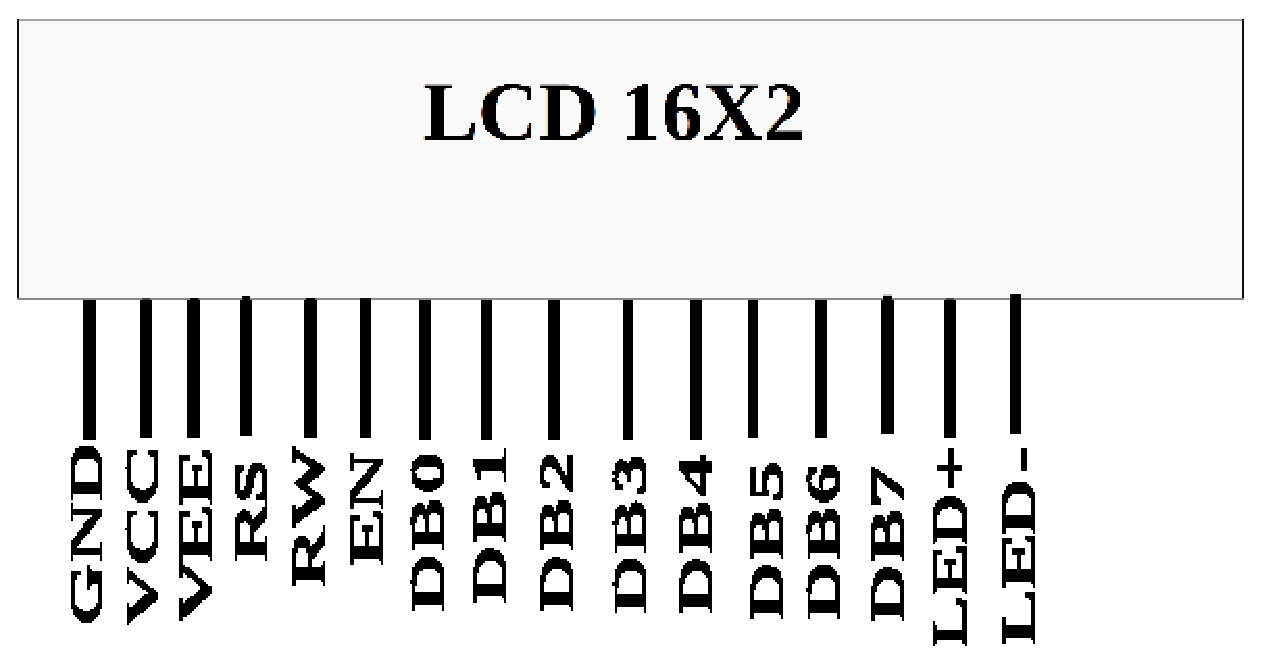
\includegraphics[width=\columnwidth]{vaman-esp32/lcd/figs/lcd.eps}
\caption{LCD pins}
\label{fig:lcd}
\end{figure}
\item
Connect the Vaman-ESP pins to LCD pins as per Table \ref{Table:1}. Make sure that all 5V sources are connected to the LCD through a 220 $\Omega$ resistance.
\item
The Vaman pin diagram is available in Fig. \ref{fig:vaman-pin_sheet}
\begin{table}[!ht]
\centering
%%%%%%%%%%%%%%%%%%%%%%%%%%%%%%%%%%%%%%%%%%%%%%%%%%%%%%%%%%%%%%%%%%%%%%
%%                                                                  %%
%%  This is the header of a LaTeX2e file exported from Gnumeric.    %%
%%                                                                  %%
%%  This file can be compiled as it stands or included in another   %%
%%  LaTeX document. The table is based on the longtable package so  %%
%%  the longtable options (headers, footers...) can be set in the   %%
%%  preamble section below (see PRAMBLE).                           %%
%%                                                                  %%
%%  To include the file in another, the following two lines must be %%
%%  in the including file:                                          %%
%%        \def\inputGnumericTable{}                                 %%
%%  at the beginning of the file and:                               %%
%%        \input{name-of-this-file.tex}                             %%
%%  where the table is to be placed. Note also that the including   %%
%%  file must use the following packages for the table to be        %%
%%  rendered correctly:                                             %%
%%    \usepackage[latin1]{inputenc}                                 %%
%%    \usepackage{color}                                            %%
%%    \usepackage{array}                                            %%
%%    \usepackage{longtable}                                        %%
%%    \usepackage{calc}                                             %%
%%    \usepackage{multirow}                                         %%
%%    \usepackage{hhline}                                           %%
%%    \usepackage{ifthen}                                           %%
%%  optionally (for landscape tables embedded in another document): %%
%%    \usepackage{lscape}                                           %%
%%                                                                  %%
%%%%%%%%%%%%%%%%%%%%%%%%%%%%%%%%%%%%%%%%%%%%%%%%%%%%%%%%%%%%%%%%%%%%%%



%%  This section checks if we are begin input into another file or  %%
%%  the file will be compiled alone. First use a macro taken from   %%
%%  the TeXbook ex 7.7 (suggestion of Han-Wen Nienhuys).            %%
\def\ifundefined#1{\expandafter\ifx\csname#1\endcsname\relax}


%%  Check for the \def token for inputed files. If it is not        %%
%%  defined, the file will be processed as a standalone and the     %%
%%  preamble will be used.                                          %%
\ifundefined{inputGnumericTable}

%%  We must be able to close or not the document at the end.        %%
	\def\gnumericTableEnd{\end{document}}


%%%%%%%%%%%%%%%%%%%%%%%%%%%%%%%%%%%%%%%%%%%%%%%%%%%%%%%%%%%%%%%%%%%%%%
%%                                                                  %%
%%  This is the PREAMBLE. Change these values to get the right      %%
%%  paper size and other niceties.                                  %%
%%                                                                  %%
%%%%%%%%%%%%%%%%%%%%%%%%%%%%%%%%%%%%%%%%%%%%%%%%%%%%%%%%%%%%%%%%%%%%%%

	\documentclass[12pt%
			  %,landscape%
                    ]{report}
       \usepackage[latin1]{inputenc}
       \usepackage{fullpage}
       \usepackage{color}
       \usepackage{array}
       \usepackage{longtable}
       \usepackage{calc}
       \usepackage{multirow}
       \usepackage{hhline}
       \usepackage{ifthen}

	\begin{document}


%%  End of the preamble for the standalone. The next section is for %%
%%  documents which are included into other LaTeX2e files.          %%
\else

%%  We are not a stand alone document. For a regular table, we will %%
%%  have no preamble and only define the closing to mean nothing.   %%
    \def\gnumericTableEnd{}

%%  If we want landscape mode in an embedded document, comment out  %%
%%  the line above and uncomment the two below. The table will      %%
%%  begin on a new page and run in landscape mode.                  %%
%       \def\gnumericTableEnd{\end{landscape}}
%       \begin{landscape}


%%  End f the else clause for this file being \input.              %%
\fi

%%%%%%%%%%%%%%%%%%%%%%%%%%%%%%%%%%%%%%%%%%%%%%%%%%%%%%%%%%%%%%%%%%%%%%
%%                                                                  %%
%%  The rest is the gnumeric table, except for the closing          %%
%%  statement. Changes below will alter the table's appearance.     %%
%%                                                                  %%
%%%%%%%%%%%%%%%%%%%%%%%%%%%%%%%%%%%%%%%%%%%%%%%%%%%%%%%%%%%%%%%%%%%%%%

\providecommand{\gnumericmathit}[1]{#1} 
%%  Uncomment the next line if you would like your numbers to be in %%
%%  italics if they are italizised in the gnumeric table.           %%
%\renewcommand{\gnumericmathit}[1]{\mathit{#1}}
\providecommand{\gnumericPB}[1]%
{\let\gnumericTemp=\\#1\let\\=\gnumericTemp\hspace{0pt}}
 \ifundefined{gnumericTableWidthDefined}
        \newlength{\gnumericTableWidth}
        \newlength{\gnumericTableWidthComplete}
        \newlength{\gnumericMultiRowLength}
        \global\def\gnumericTableWidthDefined{}
 \fi
%% The following setting protects this code from babel shorthands.  %%
 \ifthenelse{\isundefined{\languageshorthands}}{}{\languageshorthands{english}}
%%  The default table format retains the relative column widths of  %%
%%  gnumeric. They can easily be changed to c, r or l. In that case %%
%%  you may want to comment out the next line and uncomment the one %%
%%  thereafter                                                      %%
\providecommand\gnumbox{\makebox[0pt]}
%%\providecommand\gnumbox[1][]{\makebox}

%% to adjust positions in multirow situations                       %%
\setlength{\bigstrutjot}{\jot}
\setlength{\extrarowheight}{\doublerulesep}

%%  The \setlongtables command keeps column widths the same across  %%
%%  pages. Simply comment out next line for varying column widths.  %%
\setlongtables

\setlength\gnumericTableWidth{%
	45pt+%
	30pt+%
	52pt+%
	60pt+%
0pt}
\def\gumericNumCols{4}
\setlength\gnumericTableWidthComplete{\gnumericTableWidth+%
         \tabcolsep*\gumericNumCols*2+\arrayrulewidth*\gumericNumCols}
\ifthenelse{\lengthtest{\gnumericTableWidthComplete > \linewidth}}%
         {\def\gnumericScale{\ratio{\linewidth-%
                        \tabcolsep*\gumericNumCols*2-%
                        \arrayrulewidth*\gumericNumCols}%
{\gnumericTableWidth}}}%
{\def\gnumericScale{1}}

%%%%%%%%%%%%%%%%%%%%%%%%%%%%%%%%%%%%%%%%%%%%%%%%%%%%%%%%%%%%%%%%%%%%%%
%%                                                                  %%
%% The following are the widths of the various columns. We are      %%
%% defining them here because then they are easier to change.       %%
%% Depending on the cell formats we may use them more than once.    %%
%%                                                                  %%
%%%%%%%%%%%%%%%%%%%%%%%%%%%%%%%%%%%%%%%%%%%%%%%%%%%%%%%%%%%%%%%%%%%%%%

\ifthenelse{\isundefined{\gnumericColA}}{\newlength{\gnumericColA}}{}\settowidth{\gnumericColA}{\begin{tabular}{@{}p{45pt*\gnumericScale}@{}}x\end{tabular}}
\ifthenelse{\isundefined{\gnumericColB}}{\newlength{\gnumericColB}}{}\settowidth{\gnumericColB}{\begin{tabular}{@{}p{30pt*\gnumericScale}@{}}x\end{tabular}}
\ifthenelse{\isundefined{\gnumericColC}}{\newlength{\gnumericColC}}{}\settowidth{\gnumericColC}{\begin{tabular}{@{}p{52pt*\gnumericScale}@{}}x\end{tabular}}
\ifthenelse{\isundefined{\gnumericColD}}{\newlength{\gnumericColD}}{}\settowidth{\gnumericColD}{\begin{tabular}{@{}p{60pt*\gnumericScale}@{}}x\end{tabular}}

\begin{tabular}[c]{%
	b{\gnumericColA}%
	b{\gnumericColB}%
	b{\gnumericColC}%
	b{\gnumericColD}%
	}

%%%%%%%%%%%%%%%%%%%%%%%%%%%%%%%%%%%%%%%%%%%%%%%%%%%%%%%%%%%%%%%%%%%%%%
%%  The longtable options. (Caption, headers... see Goosens, p.124) %%
%	\caption{The Table Caption.}             \\	%
% \hline	% Across the top of the table.
%%  The rest of these options are table rows which are placed on    %%
%%  the first, last or every page. Use \multicolumn if you want.    %%

%%  Header for the first page.                                      %%
%	\multicolumn{4}{c}{The First Header} \\ \hline 
%	\multicolumn{1}{c}{colTag}	%Column 1
%	&\multicolumn{1}{c}{colTag}	%Column 2
%	&\multicolumn{1}{c}{colTag}	%Column 3
%	&\multicolumn{1}{c}{colTag}	\\ \hline %Last column
%	\endfirsthead

%%  The running header definition.                                  %%
%	\hline
%	\multicolumn{4}{l}{\ldots\small\slshape continued} \\ \hline
%	\multicolumn{1}{c}{colTag}	%Column 1
%	&\multicolumn{1}{c}{colTag}	%Column 2
%	&\multicolumn{1}{c}{colTag}	%Column 3
%	&\multicolumn{1}{c}{colTag}	\\ \hline %Last column
%	\endhead

%%  The running footer definition.                                  %%
%	\hline
%	\multicolumn{4}{r}{\small\slshape continued\ldots} \\
%	\endfoot

%%  The ending footer definition.                                   %%
%	\multicolumn{4}{c}{That's all folks} \\ \hline 
%	\endlastfoot
%%%%%%%%%%%%%%%%%%%%%%%%%%%%%%%%%%%%%%%%%%%%%%%%%%%%%%%%%%%%%%%%%%%%%%

\hhline{|-|-|-|-}
	 \multicolumn{1}{|p{\gnumericColA}|}%
	{\gnumericPB{\raggedright}\textbf{ESP32}}
	&\multicolumn{1}{p{\gnumericColB}|}%
	{\gnumericPB{\raggedright}\textbf{LCD Pins}}
	&\multicolumn{1}{p{\gnumericColC}|}%
	{\gnumericPB{\raggedright}\textbf{LCD Pin Label}}
	&\multicolumn{1}{p{\gnumericColD}|}%
	{\gnumericPB{\raggedright}\textbf{LCD Pin Description}}
\\
\hhline{|----|}
	 \multicolumn{1}{|p{\gnumericColA}|}%
	{\gnumericPB{\raggedright}GND}
	&\multicolumn{1}{p{\gnumericColB}|}%
	{\gnumericPB{\raggedright}1}
	&\multicolumn{1}{p{\gnumericColC}|}%
	{\gnumericPB{\raggedright}GND }
	&\multicolumn{1}{p{\gnumericColD}|}%
	{\setlength{\gnumericMultiRowLength}{0pt}%
	 \addtolength{\gnumericMultiRowLength}{\gnumericColD}%
	 \multirow{2}[1]{\gnumericMultiRowLength}{%
	 }}
\\
\hhline{|---|~}
	 \multicolumn{1}{|p{\gnumericColA}|}%
	{\gnumericPB{\raggedright}5V}
	&\multicolumn{1}{p{\gnumericColB}|}%
	{\gnumericPB{\raggedright}2}
	&\multicolumn{1}{p{\gnumericColC}|}%
	{\gnumericPB{\raggedright}Vcc}
	&\multicolumn{1}{p{\gnumericColD}|}%
	{}
\\
\hhline{|----|}
	 \multicolumn{1}{|p{\gnumericColA}|}%
	{\gnumericPB{\raggedright}GND}
	&\multicolumn{1}{p{\gnumericColB}|}%
	{\gnumericPB{\raggedright}3}
	&\multicolumn{1}{p{\gnumericColC}|}%
	{\gnumericPB{\raggedright}Vee}
	&\multicolumn{1}{p{\gnumericColD}|}%
	{\gnumericPB{\raggedright}Contrast}
\\
\hhline{|----|}
	 \multicolumn{1}{|p{\gnumericColA}|}%
	{\gnumericPB{\raggedright}GPIO 19}
	&\multicolumn{1}{p{\gnumericColB}|}%
	{\gnumericPB{\raggedright}4}
	&\multicolumn{1}{p{\gnumericColC}|}%
	{\gnumericPB{\raggedright}RS}
	&\multicolumn{1}{p{\gnumericColD}|}%
	{\gnumericPB{\raggedright}Register Select}
\\
\hhline{|----|}
	 \multicolumn{1}{|p{\gnumericColA}|}%
	{\gnumericPB{\raggedright}GND}
	&\multicolumn{1}{p{\gnumericColB}|}%
	{\gnumericPB{\raggedright}5}
	&\multicolumn{1}{p{\gnumericColC}|}%
	{\gnumericPB{\raggedright}R/W}
	&\multicolumn{1}{p{\gnumericColD}|}%
	{\gnumericPB{\raggedright}Read/Write}
\\
\hhline{|----|}
	 \multicolumn{1}{|p{\gnumericColA}|}%
	{\gnumericPB{\raggedright}GPIO 23}
	&\multicolumn{1}{p{\gnumericColB}|}%
	{\gnumericPB{\raggedright}6}
	&\multicolumn{1}{p{\gnumericColC}|}%
	{\gnumericPB{\raggedright}EN}
	&\multicolumn{1}{p{\gnumericColD}|}%
	{\gnumericPB{\raggedright}Enable}
\\
\hhline{|----|}
	 \multicolumn{1}{|p{\gnumericColA}|}%
	{\gnumericPB{\raggedright}GPIO 18}
	&\multicolumn{1}{p{\gnumericColB}|}%
	{\gnumericPB{\raggedright}11}
	&\multicolumn{1}{p{\gnumericColC}|}%
	{\gnumericPB{\raggedright}DB4}
	&\multicolumn{1}{p{\gnumericColD}|}%
	{\gnumericPB{\raggedright}Serial Connection}
\\
\hhline{|----|}
	 \multicolumn{1}{|p{\gnumericColA}|}%
	{\gnumericPB{\raggedright}GPIO 17}
	&\multicolumn{1}{p{\gnumericColB}|}%
	{\gnumericPB{\raggedright}12}
	&\multicolumn{1}{p{\gnumericColC}|}%
	{\gnumericPB{\raggedright}DB5}
	&\multicolumn{1}{p{\gnumericColD}|}%
	{\gnumericPB{\raggedright}Serial Connection}
\\
\hhline{|----|}
	 \multicolumn{1}{|p{\gnumericColA}|}%
	{\gnumericPB{\raggedright}GPIO 16}
	&\multicolumn{1}{p{\gnumericColB}|}%
	{\gnumericPB{\raggedright}13}
	&\multicolumn{1}{p{\gnumericColC}|}%
	{\gnumericPB{\raggedright}DB6}
	&\multicolumn{1}{p{\gnumericColD}|}%
	{\gnumericPB{\raggedright}Serial Connection}
\\
\hhline{|----|}
	 \multicolumn{1}{|p{\gnumericColA}|}%
	{\gnumericPB{\raggedright}GPIO 15}
	&\multicolumn{1}{p{\gnumericColB}|}%
	{\gnumericPB{\raggedright}14}
	&\multicolumn{1}{p{\gnumericColC}|}%
	{\gnumericPB{\raggedright}DB7}
	&\multicolumn{1}{p{\gnumericColD}|}%
	{\gnumericPB{\raggedright}Serial Connection}
\\
\hhline{|----|}
	 \multicolumn{1}{|p{\gnumericColA}|}%
	{\gnumericPB{\raggedright}5V}
	&\multicolumn{1}{p{\gnumericColB}|}%
	{\gnumericPB{\raggedright}15}
	&\multicolumn{1}{p{\gnumericColC}|}%
	{\gnumericPB{\raggedright}LED+}
	&\multicolumn{1}{p{\gnumericColD}|}%
	{\gnumericPB{\raggedright}Backlight}
\\
\hhline{|----|}
	 \multicolumn{1}{|p{\gnumericColA}|}%
	{\gnumericPB{\raggedright}GND}
	&\multicolumn{1}{p{\gnumericColB}|}%
	{\gnumericPB{\raggedright}16}
	&\multicolumn{1}{p{\gnumericColC}|}%
	{\gnumericPB{\raggedright}LED-}
	&\multicolumn{1}{p{\gnumericColD}|}%
	{\gnumericPB{\raggedright}Backlight}
\\
\hhline{|-|-|-|-|}
\end{tabular}

\ifthenelse{\isundefined{\languageshorthands}}{}{\languageshorthands{\languagename}}
\gnumericTableEnd

\caption{Make sure that all 5V sources are connected to the LCD through a 220 $\Omega$ resistance.}
\label{Table:1}
\end{table}

\item Execute the following code after editing the wifi credentials
\begin{lstlisting}
vaman-esp/lcd/codes/setup
\end{lstlisting}
You should see the following message
\begin{lstlisting}
Hi
This is CSP Lab
\end{lstlisting}
\item Modify the above code to display your name.
\end{enumerate}
\subsection{Measuring the resistance}
\begin{enumerate}[label=\thesection.\arabic*.,ref=\thesection.\theenumi]
\numberwithin{equation}{enumi}
\numberwithin{figure}{enumi}
\numberwithin{table}{enumi}

\item Connect the 5V pin of the Vaman-ESP32 to an extreme pin of the Breadboard 
shown in Fig. \ref{fig:breadboard}. Let this pin be $V_{cc}$.

\begin{figure}[!ht]
\centering
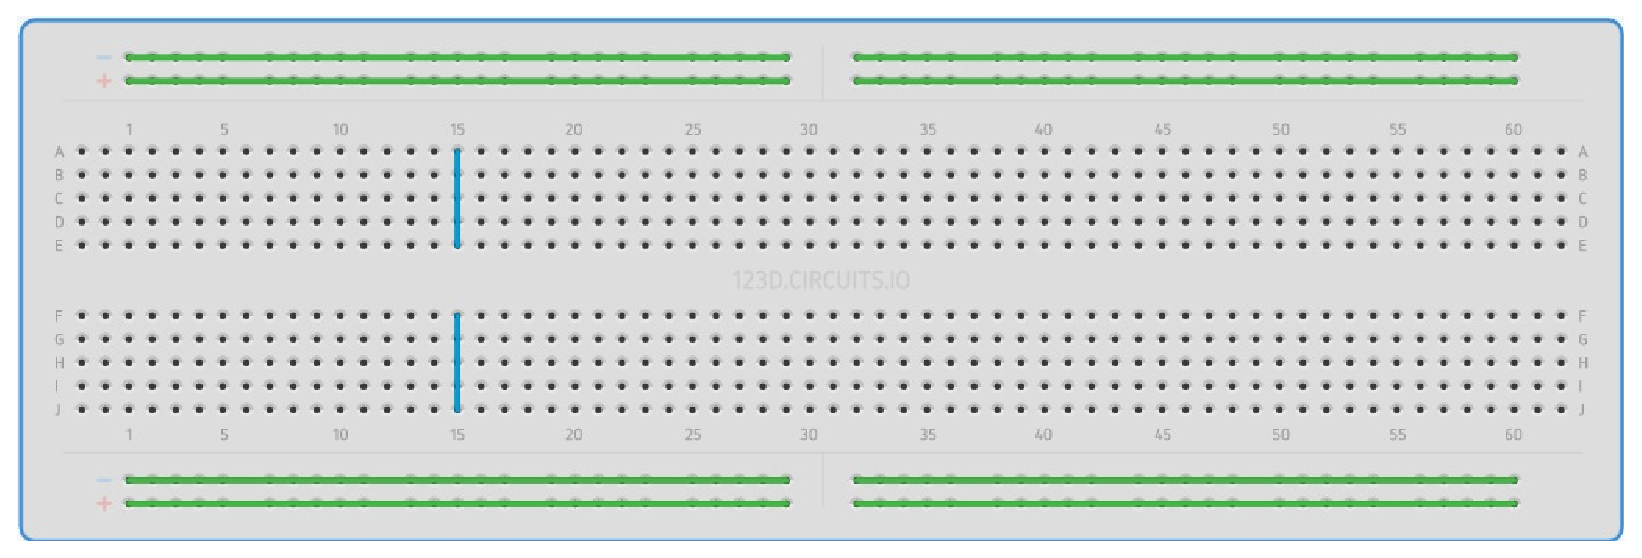
\includegraphics[width=\columnwidth]{vaman-esp32/lcd/figs/breadboard.eps}
\caption{Breadboard}
\label{fig:breadboard}
\end{figure}
%
\item
Connect the GND pin of the Vaman-ESP to the opposite extreme pin of the Breadboard.

%
\item
Let $R_1$ be the known resistor and $R_2$ be the unknown resistor.  Connect $R_1$ and $R_2$ in series such that $R_1$ is connected
to $V_{cc}$ and $R_2$ is connected to GND. Refer to Fig. \ref{fig:voltage_divider}

%
\begin{figure}[!ht]
\centering
\resizebox {\columnwidth} {!} {
\begin{circuitikz}[american]
      \draw (0,2) node[ocirc,label={[font=\footnotesize]below:$V_{CC}$}] {}
%      to[V=$V_{CC}$, invert] (0,2) % The voltage source
%      to[short] (2,2)
    to[R=$R_1 (known)$] (2,2) % The resistor
      to[R=$R_2 (unknown)$] (2,0)
      to (2,-0.5) node[ground]{GND}      ; % The resistor
%      to[short] (0,0);
\draw (2,2)   to [short, -o]   (4,2) node[label={[font=\footnotesize]above:$GPIO34$}] {};
%\draw (2,0)   to [short, -o]   (4,0);
%\draw (2,-0.5) node[ground]{GND}  to[short] (2,0);
\end{circuitikz}

%\begin{circuitikz}[american]
%      \draw (0,0)
%      to[V=$V_{CC}$, invert] (0,2) % The voltage source
%%      to[short] (2,2)
%    to[R=$R_1$] (2,2) % The resistor
%      to[R=$R_2$] (2,0) % The resistor
%      to[short] (0,0);
%\draw (2,2)   to [short, -o]   (4,2) node[label={[font=\footnotesize]above:$A3$}] {};
%%\draw (2,0)   to [short, -o]   (4,0);
%\draw (2,-0.5) node[ground]{GND}  to[short] (2,0);
%\end{circuitikz}

}
\caption{Voltage Divider}
\label{fig:voltage_divider}
\end{figure}
%
\item
Connect the junction between the two resistors to  the GPIO34 pin on the Vaman-ESP.

%
\item
Connect the Vaman-ESP to the computer so that it is powered.
\item
Execute the following code after editing the wifi credentials

\begin{lstlisting}
vaman/vaman-esp/lcd/codes/resistance
\end{lstlisting}

\end{enumerate}
\subsection{Displaying the Measured resistance on LCD and website}
\begin{enumerate}[label=\thesection.\arabic*.,ref=\thesection.\theenumi]
\numberwithin{equation}{enumi}
\numberwithin{figure}{enumi}
\numberwithin{table}{enumi}
\item The unknown resistance is measured and diplayed the measured resistance on the LCD display and also on the Vaman-ESP webserver.
\item Connect the Vaman-ESP pins to LCD pins as per Table \ref{Table:1}.
\item
Execute the following code after editing the wifi credentials

\begin{lstlisting}
vaman/vaman-esp/lcd/webserver/codes
\end{lstlisting}
\item After flashing the code to vaman-ESP, the board will be connected to the wifi credentials provided.
\item Now connect the same WiFi credentials to the mobile phone for accessing the IP address, which can be accessed by 
\begin{lstlisting}
ifconfig
nmap -sn 192.168.x.x/24
\end{lstlisting}
\item Change the IP address in the second command accordingly with the IP address provided by first command.
\item By the above commands the IP address of vaman-ESP will be diplayed.
\item Now the vaman-ESP will be hosting a webserver
\item Inorder to access the webserver type the IP address of the vaman-ESP in the web browser.
\item In the website loaded by the IP address of vaman-ESP the Unknown resitance is displayed as shown in Fig. \ref{fig:website}

\begin{figure}[!ht]
\centering
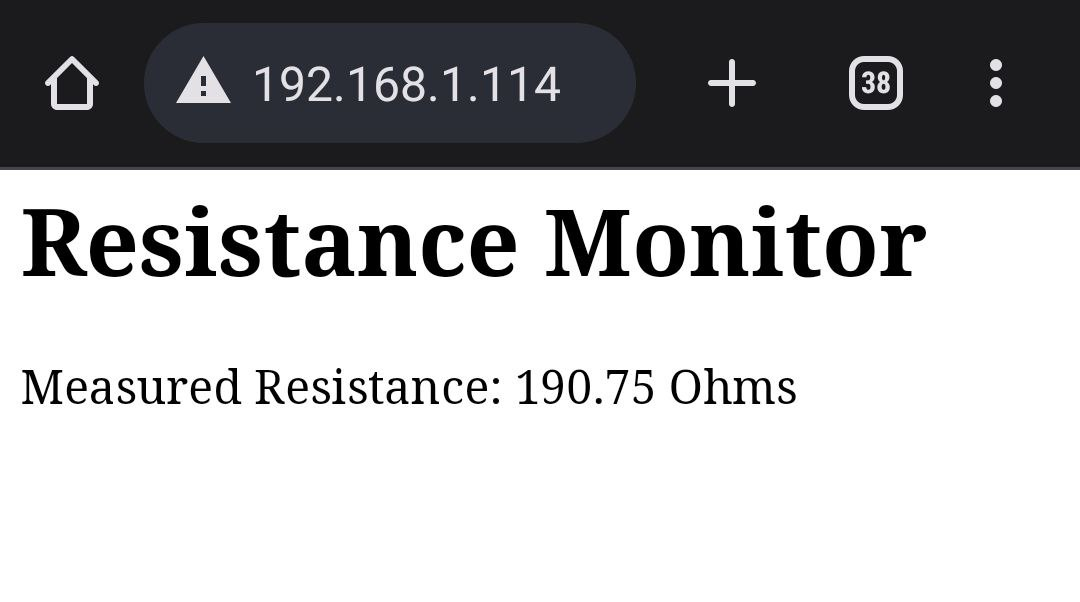
\includegraphics[width=\columnwidth]{vaman-esp32/lcd/figs/website.jpg}
\caption{Website}
\label{fig:website}
\end{figure}
\end{enumerate}

\subsection{Explanation}
\begin{enumerate}[label=\thesection.\arabic*.,ref=\thesection.\theenumi]
\numberwithin{equation}{enumi}
\numberwithin{figure}{enumi}
\numberwithin{table}{enumi}

\item We create a variable called analogPin and assign it to 0. This is because 
the voltage value we are going to read is connected to analogPin GPIO34.

\item  The 12-bit ADC can differentiate 4096 discrete voltage levels, 5 volt is 
applied to 2 resistors and the voltage sample is taken in between the resistors.
The value which we get from analogPin can be between 0 and 4095. 0 would 
represent 0 volts falls across the unknown resistor. A value of 4095 would mean 
that practically all 5 volts falls across the unknown resistor.

\item  $V_{out}$ represents the divided voltage that falls across the unknown 
resistor.

\item  The Ohm meter in this manual works on the principle of the voltage 
divider shown in Fig. \ref{fig:voltage_divider}.
%
\begin{align}
V_{out}&=\frac{R_1}{R_1+R_2}V_{in} \\
\Rightarrow R_2&=R_1\brak{\frac{V_{in}}{V_{out}}-1}
\end{align}
%
In the above, $V_{in} = 5$V, $R_1 = 220 \Omega$.
\item Repeat the exercise with another unknown resistance.
\end{enumerate}

\section{I2C Communication Between Vaman-ESP32 and Arduino}
This section describes how to setup the Vaman-ESP32 as a Master and Arduino as a
slave using I2C protocol.
\subsection{Components}
The components required are listed in \autoref{table:i2c-components}.
\begin{table}[!ht]
\centering
%%%%%%%%%%%%%%%%%%%%%%%%%%%%%%%%%%%%%%%%%%%%%%%%%%%%%%%%%%%%%%%%%%%%%%
%%                                                                  %%
%%  This is the header of a LaTeX2e file exported from Gnumeric.    %%
%%                                                                  %%
%%  This file can be compiled as it stands or included in another   %%
%%  LaTeX document. The table is based on the longtable package so  %%
%%  the longtable options (headers, footers...) can be set in the   %%
%%  preamble section below (see PRAMBLE).                           %%
%%                                                                  %%
%%  To include the file in another, the following two lines must be %%
%%  in the including file:                                          %%
%%        \def\inputGnumericTable{}                                 %%
%%  at the beginning of the file and:                               %%
%%        \input{name-of-this-file.tex}                             %%
%%  where the table is to be placed. Note also that the including   %%
%%  file must use the following packages for the table to be        %%
%%  rendered correctly:                                             %%
%%    \usepackage[latin1]{inputenc}                                 %%
%%    \usepackage{color}                                            %%
%%    \usepackage{array}                                            %%
%%    \usepackage{longtable}                                        %%
%%    \usepackage{calc}                                             %%
%%    \usepackage{multirow}                                         %%
%%    \usepackage{hhline}                                           %%
%%    \usepackage{ifthen}                                           %%
%%  optionally (for landscape tables embedded in another document): %%
%%    \usepackage{lscape}                                           %%
%%                                                                  %%
%%%%%%%%%%%%%%%%%%%%%%%%%%%%%%%%%%%%%%%%%%%%%%%%%%%%%%%%%%%%%%%%%%%%%%



%%  This section checks if we are begin input into another file or  %%
%%  the file will be compiled alone. First use a macro taken from   %%
%%  the TeXbook ex 7.7 (suggestion of Han-Wen Nienhuys).            %%
\def\ifundefined#1{\expandafter\ifx\csname#1\endcsname\relax}


%%  Check for the \def token for inputed files. If it is not        %%
%%  defined, the file will be processed as a standalone and the     %%
%%  preamble will be used.                                          %%
\ifundefined{inputGnumericTable}

%%  We must be able to close or not the document at the end.        %%
	\def\gnumericTableEnd{\end{document}}


%%%%%%%%%%%%%%%%%%%%%%%%%%%%%%%%%%%%%%%%%%%%%%%%%%%%%%%%%%%%%%%%%%%%%%
%%                                                                  %%
%%  This is the PREAMBLE. Change these values to get the right      %%
%%  paper size and other niceties.                                  %%
%%                                                                  %%
%%%%%%%%%%%%%%%%%%%%%%%%%%%%%%%%%%%%%%%%%%%%%%%%%%%%%%%%%%%%%%%%%%%%%%

	\documentclass[12pt%
			  %,landscape%
                    ]{report}
       \usepackage[latin1]{inputenc}
       \usepackage{fullpage}
       \usepackage{color}
       \usepackage{array}
       \usepackage{longtable}
       \usepackage{calc}
       \usepackage{multirow}
       \usepackage{hhline}
       \usepackage{ifthen}

	\begin{document}


%%  End of the preamble for the standalone. The next section is for %%
%%  documents which are included into other LaTeX2e files.          %%
\else

%%  We are not a stand alone document. For a regular table, we will %%
%%  have no preamble and only define the closing to mean nothing.   %%
    \def\gnumericTableEnd{}

%%  If we want landscape mode in an embedded document, comment out  %%
%%  the line above and uncomment the two below. The table will      %%
%%  begin on a new page and run in landscape mode.                  %%
%       \def\gnumericTableEnd{\end{landscape}}
%       \begin{landscape}


%%  End of the else clause for this file being \input.              %%
\fi

%%%%%%%%%%%%%%%%%%%%%%%%%%%%%%%%%%%%%%%%%%%%%%%%%%%%%%%%%%%%%%%%%%%%%%
%%                                                                  %%
%%  The rest is the gnumeric table, except for the closing          %%
%%  statement. Changes below will alter the table's appearance.     %%
%%                                                                  %%
%%%%%%%%%%%%%%%%%%%%%%%%%%%%%%%%%%%%%%%%%%%%%%%%%%%%%%%%%%%%%%%%%%%%%%

\providecommand{\gnumericmathit}[1]{#1} 
%%  Uncomment the next line if you would like your numbers to be in %%
%%  italics if they are italizised in the gnumeric table.           %%
%\renewcommand{\gnumericmathit}[1]{\mathit{#1}}
\providecommand{\gnumericPB}[1]%
{\let\gnumericTemp=\\#1\let\\=\gnumericTemp\hspace{0pt}}
 \ifundefined{gnumericTableWidthDefined}
        \newlength{\gnumericTableWidth}
        \newlength{\gnumericTableWidthComplete}
        \newlength{\gnumericMultiRowLength}
        \global\def\gnumericTableWidthDefined{}
 \fi
%% The following setting protects this code from babel shorthands.  %%
 \ifthenelse{\isundefined{\languageshorthands}}{}{\languageshorthands{english}}
%%  The default table format retains the relative column widths of  %%
%%  gnumeric. They can easily be changed to c, r or l. In that case %%
%%  you may want to comment out the next line and uncomment the one %%
%%  thereafter                                                      %%
\providecommand\gnumbox{\makebox[0pt]}
%%\providecommand\gnumbox[1][]{\makebox}

%% to adjust positions in multirow situations                       %%
\setlength{\bigstrutjot}{\jot}
\setlength{\extrarowheight}{\doublerulesep}

%%  The \setlongtables command keeps column widths the same across  %%
%%  pages. Simply comment out next line for varying column widths.  %%
\setlongtables

\setlength\gnumericTableWidth{%
	82pt+%
	52pt+%
	55pt+%
0pt}
\def\gumericNumCols{3}
\setlength\gnumericTableWidthComplete{\gnumericTableWidth+%
         \tabcolsep*\gumericNumCols*2+\arrayrulewidth*\gumericNumCols}
\ifthenelse{\lengthtest{\gnumericTableWidthComplete > \linewidth}}%
         {\def\gnumericScale{\ratio{\linewidth-%
                        \tabcolsep*\gumericNumCols*2-%
                        \arrayrulewidth*\gumericNumCols}%
{\gnumericTableWidth}}}%
{\def\gnumericScale{1}}

%%%%%%%%%%%%%%%%%%%%%%%%%%%%%%%%%%%%%%%%%%%%%%%%%%%%%%%%%%%%%%%%%%%%%%
%%                                                                  %%
%% The following are the widths of the various columns. We are      %%
%% defining them here because then they are easier to change.       %%
%% Depending on the cell formats we may use them more than once.    %%
%%                                                                  %%
%%%%%%%%%%%%%%%%%%%%%%%%%%%%%%%%%%%%%%%%%%%%%%%%%%%%%%%%%%%%%%%%%%%%%%

\ifthenelse{\isundefined{\gnumericColA}}{\newlength{\gnumericColA}}{}\settowidth{\gnumericColA}{\begin{tabular}{@{}p{82pt*\gnumericScale}@{}}x\end{tabular}}
\ifthenelse{\isundefined{\gnumericColB}}{\newlength{\gnumericColB}}{}\settowidth{\gnumericColB}{\begin{tabular}{@{}p{52pt*\gnumericScale}@{}}x\end{tabular}}
\ifthenelse{\isundefined{\gnumericColC}}{\newlength{\gnumericColC}}{}\settowidth{\gnumericColC}{\begin{tabular}{@{}p{55pt*\gnumericScale}@{}}x\end{tabular}}

\begin{tabular}[c]{%
	b{\gnumericColA}%
	b{\gnumericColB}%
	b{\gnumericColC}%
	}

%%%%%%%%%%%%%%%%%%%%%%%%%%%%%%%%%%%%%%%%%%%%%%%%%%%%%%%%%%%%%%%%%%%%%%
%%  The longtable options. (Caption, headers... see Goosens, p.124) %%
%	\caption{The Table Caption.}             \\	%
% \hline	% Across the top of the table.
%%  The rest of these options are table rows which are placed on    %%
%%  the first, last or every page. Use \multicolumn if you want.    %%

%%  Header for the first page.                                      %%
%	\multicolumn{3}{c}{The First Header} \\ \hline 
%	\multicolumn{1}{c}{colTag}	%Column 1
%	&\multicolumn{1}{c}{colTag}	%Column 2
%	&\multicolumn{1}{c}{colTag}	\\ \hline %Last column
%	\endfirsthead

%%  The running header definition.                                  %%
%	\hline
%	\multicolumn{3}{l}{\ldots\small\slshape continued} \\ \hline
%	\multicolumn{1}{c}{colTag}	%Column 1
%	&\multicolumn{1}{c}{colTag}	%Column 2
%	&\multicolumn{1}{c}{colTag}	\\ \hline %Last column
%	\endhead

%%  The running footer definition.                                  %%
%	\hline
%	\multicolumn{3}{r}{\small\slshape continued\ldots} \\
%	\endfoot

%%  The ending footer definition.                                   %%
%	\multicolumn{3}{c}{That's all folks} \\ \hline 
%	\endlastfoot
%%%%%%%%%%%%%%%%%%%%%%%%%%%%%%%%%%%%%%%%%%%%%%%%%%%%%%%%%%%%%%%%%%%%%%

\hhline{|-|-|-}
	 \multicolumn{1}{|p{\gnumericColA}|}%
	{\gnumericPB{\centering}\textbf{Component}}
	&\multicolumn{1}{p{\gnumericColB}|}%
	{\gnumericPB{\centering}\textbf{Value}}
	&\multicolumn{1}{p{\gnumericColC}|}%
	{\gnumericPB{\centering}\textbf{Quantity}}
\\
\hhline{|---|}
	 \multicolumn{1}{|p{\gnumericColA}|}%
	{\gnumericPB{\centering}\gnumbox{ESP32}}
	&\multicolumn{1}{p{\gnumericColB}|}%
	{Devkit V1}
	&\multicolumn{1}{p{\gnumericColC}|}%
	{\gnumericPB{\centering}\gnumbox{1}}
\\
\hhline{|---|}
	 \multicolumn{1}{|p{\gnumericColA}|}%
	{\gnumericPB{\centering}\gnumbox{Arduino}}
	&\multicolumn{1}{p{\gnumericColB}|}%
	{UNO}
	&\multicolumn{1}{p{\gnumericColC}|}%
	{\gnumericPB{\centering}\gnumbox{1}}
\\
\hhline{|---|}
	 \multicolumn{1}{|p{\gnumericColA}|}%
	{\gnumericPB{\centering}\gnumbox{}Connecting Wires}
	&\multicolumn{1}{p{\gnumericColB}|}%
	{\gnumericPB{\centering}\gnumbox{}}
	&\multicolumn{1}{p{\gnumericColC}|}%
	{\gnumericPB{\centering}\gnumbox{30}}
	\\
\hhline{|---|}
	 \multicolumn{1}{|p{\gnumericColA}|}%
	{\gnumericPB{\centering}\gnumbox{}LCD}
	&\multicolumn{1}{p{\gnumericColB}|}%
	{\gnumericPB{\centering}\gnumbox{}16 X 2}
	&\multicolumn{1}{p{\gnumericColC}|}%
	{\gnumericPB{\centering}\gnumbox{1}}
\\
\hhline{|-|-|-|}
\end{tabular}

\ifthenelse{\isundefined{\languageshorthands}}{}{\languageshorthands{\languagename}}
\gnumericTableEnd

\caption{Components.}
\label{table:i2c-components}
\end{table}

\subsection{Setting up the Master and Slave}
\begin{enumerate}
\item Connect the Vaman-ESP32 pins to Arduino pins as per \autoref{Table:1
Arduino-ESP}.
\begin{table}[!ht]
\centering
%%%%%%%%%%%%%%%%%%%%%%%%%%%%%%%%%%%%%%%%%%%%%%%%%%%%%%%%%%%%%%%%%%%%%%
%%                                                                  %%
%%  This is the header of a LaTeX2e file exported from Gnumeric.    %%
%%                                                                  %%
%%  This file can be compiled as it stands or included in another   %%
%%  LaTeX document. The table is based on the longtable package so  %%
%%  the longtable options (headers, footers...) can be set in the   %%
%%  preamble section below (see PRAMBLE).                           %%
%%                                                                  %%
%%  To include the file in another, the following two lines must be %%
%%  in the including file:                                          %%
%%        \def\inputGnumericTable{}                                 %%
%%  at the beginning of the file and:                               %%
%%        \input{name-of-this-file.tex}                             %%
%%  where the table is to be placed. Note also that the including   %%
%%  file must use the following packages for the table to be        %%
%%  rendered correctly:                                             %%
%%    \usepackage[latin1]{inputenc}                                 %%
%%    \usepackage{color}                                            %%
%%    \usepackage{array}                                            %%
%%    \usepackage{longtable}                                        %%
%%    \usepackage{calc}                                             %%
%%    \usepackage{multirow}                                         %%
%%    \usepackage{hhline}                                           %%
%%    \usepackage{ifthen}                                           %%
%%  optionally (for landscape tables embedded in another document): %%
%%    \usepackage{lscape}                                           %%
%%                                                                  %%
%%%%%%%%%%%%%%%%%%%%%%%%%%%%%%%%%%%%%%%%%%%%%%%%%%%%%%%%%%%%%%%%%%%%%%



%%  This section checks if we are begin input into another file or  %%
%%  the file will be compiled alone. First use a macro taken from   %%
%%  the TeXbook ex 7.7 (suggestion of Han-Wen Nienhuys).            %%
\def\ifundefined#1{\expandafter\ifx\csname#1\endcsname\relax}


%%  Check for the \def token for inputed files. If it is not        %%
%%  defined, the file will be processed as a standalone and the     %%
%%  preamble will be used.                                          %%
\ifundefined{inputGnumericTable}

%%  We must be able to close or not the document at the end.        %%
	\def\gnumericTableEnd{\end{document}}


%%%%%%%%%%%%%%%%%%%%%%%%%%%%%%%%%%%%%%%%%%%%%%%%%%%%%%%%%%%%%%%%%%%%%%
%%                                                                  %%
%%  This is the PREAMBLE. Change these values to get the right      %%
%%  paper size and other niceties.                                  %%
%%                                                                  %%
%%%%%%%%%%%%%%%%%%%%%%%%%%%%%%%%%%%%%%%%%%%%%%%%%%%%%%%%%%%%%%%%%%%%%%

	\documentclass[12pt%
			  %,landscape%
                    ]{report}
       \usepackage[latin1]{inputenc}
       \usepackage{fullpage}
       \usepackage{color}
       \usepackage{array}
       \usepackage{longtable}
       \usepackage{calc}
       \usepackage{multirow}
       \usepackage{hhline}
       \usepackage{ifthen}

	\begin{document}


%%  End of the preamble for the standalone. The next section is for %%
%%  documents which are included into other LaTeX2e files.          %%
\else

%%  We are not a stand alone document. For a regular table, we will %%
%%  have no preamble and only define the closing to mean nothing.   %%
    \def\gnumericTableEnd{}

%%  If we want landscape mode in an embedded document, comment out  %%
%%  the line above and uncomment the two below. The table will      %%
%%  begin on a new page and run in landscape mode.                  %%
%       \def\gnumericTableEnd{\end{landscape}}
%       \begin{landscape}


%%  End of the else clause for this file being \input.              %%
\fi

%%%%%%%%%%%%%%%%%%%%%%%%%%%%%%%%%%%%%%%%%%%%%%%%%%%%%%%%%%%%%%%%%%%%%%
%%                                                                  %%
%%  The rest is the gnumeric table, except for the closing          %%
%%  statement. Changes below will alter the table's appearance.     %%
%%                                                                  %%
%%%%%%%%%%%%%%%%%%%%%%%%%%%%%%%%%%%%%%%%%%%%%%%%%%%%%%%%%%%%%%%%%%%%%%

\providecommand{\gnumericmathit}[1]{#1} 
%%  Uncomment the next line if you would like your numbers to be in %%
%%  italics if they are italizised in the gnumeric table.           %%
%\renewcommand{\gnumericmathit}[1]{\mathit{#1}}
\providecommand{\gnumericPB}[1]%
{\let\gnumericTemp=\\#1\let\\=\gnumericTemp\hspace{0pt}}
 \ifundefined{gnumericTableWidthDefined}
        \newlength{\gnumericTableWidth}
        \newlength{\gnumericTableWidthComplete}
        \newlength{\gnumericMultiRowLength}
        \global\def\gnumericTableWidthDefined{}
 \fi
%% The following setting protects this code from babel shorthands.  %%
 \ifthenelse{\isundefined{\languageshorthands}}{}{\languageshorthands{english}}
%%  The default table format retains the relative column widths of  %%
%%  gnumeric. They can easily be changed to c, r or l. In that case %%
%%  you may want to comment out the next line and uncomment the one %%
%%  thereafter                                                      %%
\providecommand\gnumbox{\makebox[0pt]}
%%\providecommand\gnumbox[1][]{\makebox}

%% to adjust positions in multirow situations                       %%
\setlength{\bigstrutjot}{\jot}
\setlength{\extrarowheight}{\doublerulesep}

%%  The \setlongtables command keeps column widths the same across  %%
%%  pages. Simply comment out next line for varying column widths.  %%
\setlongtables

\setlength\gnumericTableWidth{%
	45pt+%
	52pt+%
	52pt+%
0pt}
\def\gumericNumCols{3}
\setlength\gnumericTableWidthComplete{\gnumericTableWidth+%
         \tabcolsep*\gumericNumCols*2+\arrayrulewidth*\gumericNumCols}
\ifthenelse{\lengthtest{\gnumericTableWidthComplete > \linewidth}}%
         {\def\gnumericScale{\ratio{\linewidth-%
                        \tabcolsep*\gumericNumCols*2-%
                        \arrayrulewidth*\gumericNumCols}%
{\gnumericTableWidth}}}%
{\def\gnumericScale{1}}

%%%%%%%%%%%%%%%%%%%%%%%%%%%%%%%%%%%%%%%%%%%%%%%%%%%%%%%%%%%%%%%%%%%%%%
%%                                                                  %%
%% The following are the widths of the various columns. We are      %%
%% defining them here because then they are easier to change.       %%
%% Depending on the cell formats we may use them more than once.    %%
%%                                                                  %%
%%%%%%%%%%%%%%%%%%%%%%%%%%%%%%%%%%%%%%%%%%%%%%%%%%%%%%%%%%%%%%%%%%%%%%

\ifthenelse{\isundefined{\gnumericColA}}{\newlength{\gnumericColA}}{}\settowidth{\gnumericColA}{\begin{tabular}{@{}p{45pt*\gnumericScale}@{}}x\end{tabular}}
\ifthenelse{\isundefined{\gnumericColB}}{\newlength{\gnumericColB}}{}\settowidth{\gnumericColB}{\begin{tabular}{@{}p{52pt*\gnumericScale}@{}}x\end{tabular}}
\ifthenelse{\isundefined{\gnumericColC}}{\newlength{\gnumericColC}}{}\settowidth{\gnumericColC}{\begin{tabular}{@{}p{52pt*\gnumericScale}@{}}x\end{tabular}}

\begin{tabular}[c]{%
	b{\gnumericColA}%
	b{\gnumericColB}%
	b{\gnumericColC}%
	}

%%%%%%%%%%%%%%%%%%%%%%%%%%%%%%%%%%%%%%%%%%%%%%%%%%%%%%%%%%%%%%%%%%%%%%
%%  The longtable options. (Caption, headers... see Goosens, p.124) %%
%	\caption{The Table Caption.}             \\	%
% \hline	% Across the top of the table.
%%  The rest of these options are table rows which are placed on    %%
%%  the first, last or every page. Use \multicolumn if you want.    %%

%%  Header for the first page.                                      %%
%	\multicolumn{4}{c}{The First Header} \\ \hline 
%	\multicolumn{1}{c}{colTag}	%Column 1
%	&\multicolumn{1}{c}{colTag}	%Column 2
%	&\multicolumn{1}{c}{colTag}	%Column 3
%	&\multicolumn{1}{c}{colTag}	\\ \hline %Last column
%	\endfirsthead

%%  The running header definition.                                  %%
%	\hline
%	\multicolumn{4}{l}{\ldots\small\slshape continued} \\ \hline
%	\multicolumn{1}{c}{colTag}	%Column 1
%	&\multicolumn{1}{c}{colTag}	%Column 2
%	&\multicolumn{1}{c}{colTag}	%Column 3
%	&\multicolumn{1}{c}{colTag}	\\ \hline %Last column
%	\endhead

%%  The running footer definition.                                  %%
%	\hline
%	\multicolumn{4}{r}{\small\slshape continued\ldots} \\
%	\endfoot

%%  The ending footer definition.                                   %%
%	\multicolumn{4}{c}{That's all folks} \\ \hline 
%	\endlastfoot
%%%%%%%%%%%%%%%%%%%%%%%%%%%%%%%%%%%%%%%%%%%%%%%%%%%%%%%%%%%%%%%%%%%%%%

\hhline{|-|-|-|}
	 \multicolumn{1}{|p{\gnumericColA}|}%
	{\gnumericPB{\raggedright}\textbf{I2C}}
	&\multicolumn{1}{p{\gnumericColB}|}%
	{\gnumericPB{\raggedright}\textbf{ESP32}}
	&\multicolumn{1}{p{\gnumericColC}|}%
	{\gnumericPB{\raggedright}\textbf{Arduino}}
\\
\hhline{|---|}
	 \multicolumn{1}{|p{\gnumericColA}|}%
	{\gnumericPB{\raggedright}SDA}
	&\multicolumn{1}{p{\gnumericColB}|}%
	{\gnumericPB{\raggedright}GPIO 21}
	&\multicolumn{1}{p{\gnumericColC}|}%
	{A4}
\\
\hhline{|---|}
	 \multicolumn{1}{|p{\gnumericColA}|}%
	{\gnumericPB{\raggedright}SDC}
	&\multicolumn{1}{p{\gnumericColB}|}%
	{\gnumericPB{\raggedright}GPIO 22}
	&\multicolumn{1}{p{\gnumericColC}|}%
	{\gnumericPB{\raggedright}A5}
\\
\hhline{|---|}
	 \multicolumn{1}{|p{\gnumericColA}|}%
	{\gnumericPB{\raggedright}}
	&\multicolumn{1}{p{\gnumericColB}|}%
	{\gnumericPB{\raggedright}VCC}
	&\multicolumn{1}{p{\gnumericColC}|}%
	{\gnumericPB{\raggedright}VCC}
\\
\hhline{|---|}
	 \multicolumn{1}{|p{\gnumericColA}|}%
	{\gnumericPB{\raggedright}}
	&\multicolumn{1}{p{\gnumericColB}|}%
	{\gnumericPB{\raggedright}GND}
	&\multicolumn{1}{p{\gnumericColC}|}%
	{\gnumericPB{\raggedright}GND}
	
\\
\hhline{|-|-|-|}
\end{tabular}

\ifthenelse{\isundefined{\languageshorthands}}{}{\languageshorthands{\languagename}}
\gnumericTableEnd

\caption{Connections Between Arduino and Vaman-ESP32.}
\label{Table:1 Arduino-ESP}
\end{table}

\item Connect the Vaman-ESP32 pins to LCD pins as per \autoref{Table:1}.

\item The Vaman pin diagram is available in \autoref{fig:vaman-pin_sheet}.

\item Configure Arduino Uno as a Slave using the following PlatformIO project.
\begin{lstlisting}
vaman-esp32/i2c/codes/I2C_Sender_Arduino
\end{lstlisting}
\item
Now configure Vaman-ESP32 as a Master using the following PlatformIO project.
\begin{lstlisting}
vaman-esp32/i2c/codes/I2C_Reciever_ESP32
\end{lstlisting}

\end{enumerate}
\section{I2C Communication between Vaman-ESP32 and Two Arduinos}
This section describes how to setup the Vaman-ESP32 as a master and two Arduinos
as a slave using I2C protocol. The two unknown resistances are measured by using
two Arduinos and sending those two resistance values to Vaman-ESP32 through I2C
and displaying the unkwnown resistances on ESP32 webserver.
\subsection{Components}
The components required are listed in \autoref{table:i2c-resistance-components}.
\begin{table}[!ht]
\centering
%%%%%%%%%%%%%%%%%%%%%%%%%%%%%%%%%%%%%%%%%%%%%%%%%%%%%%%%%%%%%%%%%%%%%%
%%                                                                  %%
%%  This is the header of a LaTeX2e file exported from Gnumeric.    %%
%%                                                                  %%
%%  This file can be compiled as it stands or included in another   %%
%%  LaTeX document. The table is based on the longtable package so  %%
%%  the longtable options (headers, footers...) can be set in the   %%
%%  preamble section below (see PRAMBLE).                           %%
%%                                                                  %%
%%  To include the file in another, the following two lines must be %%
%%  in the including file:                                          %%
%%        \def\inputGnumericTable{}                                 %%
%%  at the beginning of the file and:                               %%
%%        \input{name-of-this-file.tex}                             %%
%%  where the table is to be placed. Note also that the including   %%
%%  file must use the following packages for the table to be        %%
%%  rendered correctly:                                             %%
%%    \usepackage[latin1]{inputenc}                                 %%
%%    \usepackage{color}                                            %%
%%    \usepackage{array}                                            %%
%%    \usepackage{longtable}                                        %%
%%    \usepackage{calc}                                             %%
%%    \usepackage{multirow}                                         %%
%%    \usepackage{hhline}                                           %%
%%    \usepackage{ifthen}                                           %%
%%  optionally (for landscape tables embedded in another document): %%
%%    \usepackage{lscape}                                           %%
%%                                                                  %%
%%%%%%%%%%%%%%%%%%%%%%%%%%%%%%%%%%%%%%%%%%%%%%%%%%%%%%%%%%%%%%%%%%%%%%



%%  This section checks if we are begin input into another file or  %%
%%  the file will be compiled alone. First use a macro taken from   %%
%%  the TeXbook ex 7.7 (suggestion of Han-Wen Nienhuys).            %%
\def\ifundefined#1{\expandafter\ifx\csname#1\endcsname\relax}


%%  Check for the \def token for inputed files. If it is not        %%
%%  defined, the file will be processed as a standalone and the     %%
%%  preamble will be used.                                          %%
\ifundefined{inputGnumericTable}

%%  We must be able to close or not the document at the end.        %%
	\def\gnumericTableEnd{\end{document}}


%%%%%%%%%%%%%%%%%%%%%%%%%%%%%%%%%%%%%%%%%%%%%%%%%%%%%%%%%%%%%%%%%%%%%%
%%                                                                  %%
%%  This is the PREAMBLE. Change these values to get the right      %%
%%  paper size and other niceties.                                  %%
%%                                                                  %%
%%%%%%%%%%%%%%%%%%%%%%%%%%%%%%%%%%%%%%%%%%%%%%%%%%%%%%%%%%%%%%%%%%%%%%

	\documentclass[12pt%
			  %,landscape%
                    ]{report}
       \usepackage[latin1]{inputenc}
       \usepackage{fullpage}
       \usepackage{color}
       \usepackage{array}
       \usepackage{longtable}
       \usepackage{calc}
       \usepackage{multirow}
       \usepackage{hhline}
       \usepackage{ifthen}

	\begin{document}


%%  End of the preamble for the standalone. The next section is for %%
%%  documents which are included into other LaTeX2e files.          %%
\else

%%  We are not a stand alone document. For a regular table, we will %%
%%  have no preamble and only define the closing to mean nothing.   %%
    \def\gnumericTableEnd{}

%%  If we want landscape mode in an embedded document, comment out  %%
%%  the line above and uncomment the two below. The table will      %%
%%  begin on a new page and run in landscape mode.                  %%
%       \def\gnumericTableEnd{\end{landscape}}
%       \begin{landscape}


%%  End of the else clause for this file being \input.              %%
\fi

%%%%%%%%%%%%%%%%%%%%%%%%%%%%%%%%%%%%%%%%%%%%%%%%%%%%%%%%%%%%%%%%%%%%%%
%%                                                                  %%
%%  The rest is the gnumeric table, except for the closing          %%
%%  statement. Changes below will alter the table's appearance.     %%
%%                                                                  %%
%%%%%%%%%%%%%%%%%%%%%%%%%%%%%%%%%%%%%%%%%%%%%%%%%%%%%%%%%%%%%%%%%%%%%%

\providecommand{\gnumericmathit}[1]{#1} 
%%  Uncomment the next line if you would like your numbers to be in %%
%%  italics if they are italizised in the gnumeric table.           %%
%\renewcommand{\gnumericmathit}[1]{\mathit{#1}}
\providecommand{\gnumericPB}[1]%
{\let\gnumericTemp=\\#1\let\\=\gnumericTemp\hspace{0pt}}
 \ifundefined{gnumericTableWidthDefined}
        \newlength{\gnumericTableWidth}
        \newlength{\gnumericTableWidthComplete}
        \newlength{\gnumericMultiRowLength}
        \global\def\gnumericTableWidthDefined{}
 \fi
%% The following setting protects this code from babel shorthands.  %%
 \ifthenelse{\isundefined{\languageshorthands}}{}{\languageshorthands{english}}
%%  The default table format retains the relative column widths of  %%
%%  gnumeric. They can easily be changed to c, r or l. In that case %%
%%  you may want to comment out the next line and uncomment the one %%
%%  thereafter                                                      %%
\providecommand\gnumbox{\makebox[0pt]}
%%\providecommand\gnumbox[1][]{\makebox}

%% to adjust positions in multirow situations                       %%
\setlength{\bigstrutjot}{\jot}
\setlength{\extrarowheight}{\doublerulesep}

%%  The \setlongtables command keeps column widths the same across  %%
%%  pages. Simply comment out next line for varying column widths.  %%
\setlongtables

\setlength\gnumericTableWidth{%
	152pt+%
	60pt+%
	65pt+%
0pt}
\def\gumericNumCols{3}
\setlength\gnumericTableWidthComplete{\gnumericTableWidth+%
         \tabcolsep*\gumericNumCols*2+\arrayrulewidth*\gumericNumCols}
\ifthenelse{\lengthtest{\gnumericTableWidthComplete > \linewidth}}%
         {\def\gnumericScale{1*\ratio{\linewidth-%
                        \tabcolsep*\gumericNumCols*2-%
                        \arrayrulewidth*\gumericNumCols}%
{\gnumericTableWidth}}}%
{\def\gnumericScale{1}}

%%%%%%%%%%%%%%%%%%%%%%%%%%%%%%%%%%%%%%%%%%%%%%%%%%%%%%%%%%%%%%%%%%%%%%
%%                                                                  %%
%% The following are the widths of the various columns. We are      %%
%% defining them here because then they are easier to change.       %%
%% Depending on the cell formats we may use them more than once.    %%
%%                                                                  %%
%%%%%%%%%%%%%%%%%%%%%%%%%%%%%%%%%%%%%%%%%%%%%%%%%%%%%%%%%%%%%%%%%%%%%%

\ifthenelse{\isundefined{\gnumericColA}}{\newlength{\gnumericColA}}{}\settowidth{\gnumericColA}{\begin{tabular}{@{}p{152pt*\gnumericScale}@{}}x\end{tabular}}
\ifthenelse{\isundefined{\gnumericColB}}{\newlength{\gnumericColB}}{}\settowidth{\gnumericColB}{\begin{tabular}{@{}p{60pt*\gnumericScale}@{}}x\end{tabular}}
\ifthenelse{\isundefined{\gnumericColC}}{\newlength{\gnumericColC}}{}\settowidth{\gnumericColC}{\begin{tabular}{@{}p{65pt*\gnumericScale}@{}}x\end{tabular}}

\begin{longtable}[c]{%
	b{\gnumericColA}%
	b{\gnumericColB}%
	b{\gnumericColC}%
	}

%%%%%%%%%%%%%%%%%%%%%%%%%%%%%%%%%%%%%%%%%%%%%%%%%%%%%%%%%%%%%%%%%%%%%%
%%  The longtable options. (Caption, headers... see Goosens, p.124) %%
%	\caption{The Table Caption.}             \\	%
% \hline	% Across the top of the table.
%%  The rest of these options are table rows which are placed on    %%
%%  the first, last or every page. Use \multicolumn if you want.    %%

%%  Header for the first page.                                      %%
%	\multicolumn{3}{c}{The First Header} \\ \hline 
%	\multicolumn{1}{c}{colTag}	%Column 1
%	&\multicolumn{1}{c}{colTag}	%Column 2
%	&\multicolumn{1}{c}{colTag}	\\ \hline %Last column
%	\endfirsthead

%%  The running header definition.                                  %%
%	\hline
%	\multicolumn{3}{l}{\ldots\small\slshape continued} \\ \hline
%	\multicolumn{1}{c}{colTag}	%Column 1
%	&\multicolumn{1}{c}{colTag}	%Column 2
%	&\multicolumn{1}{c}{colTag}	\\ \hline %Last column
%	\endhead

%%  The running footer definition.                                  %%
%	\hline
%	\multicolumn{3}{r}{\small\slshape continued\ldots} \\
%	\endfoot

%%  The ending footer definition.                                   %%
%	\multicolumn{3}{c}{That's all folks} \\ \hline 
%	\endlastfoot
%%%%%%%%%%%%%%%%%%%%%%%%%%%%%%%%%%%%%%%%%%%%%%%%%%%%%%%%%%%%%%%%%%%%%%

\hhline{|-|-|-}
	 \multicolumn{1}{|p{\gnumericColA}|}%
	{\gnumericPB{\centering}\textbf{Component}}
	&\multicolumn{1}{p{\gnumericColB}|}%
	{\gnumericPB{\centering}\textbf{Value}}
	&\multicolumn{1}{p{\gnumericColC}|}%
	{\gnumericPB{\centering}\textbf{Quantity}}
\\
\hhline{|---|}
	 \multicolumn{1}{|p{\gnumericColA}|}%
	{\setlength{\gnumericMultiRowLength}{0pt}%
	 \addtolength{\gnumericMultiRowLength}{\gnumericColA}%
	 \multirow{2}[1]{\gnumericMultiRowLength}{\parbox{\gnumericMultiRowLength}{%
	 \gnumericPB{\centering}Resistor}}}
	&\multicolumn{1}{p{\gnumericColB}|}%
	{\gnumericPB{\centering}220 Ohm}
	&\multicolumn{1}{p{\gnumericColC}|}%
	{\gnumericPB{\centering}1}
\\
\hhline{~|--|}
	 \multicolumn{1}{|p{\gnumericColA}|}%
	{}
	&\multicolumn{1}{p{\gnumericColB}|}%
	{\gnumericPB{\centering}\gnumbox{2K Ohm}}
	&\multicolumn{1}{p{\gnumericColC}|}%
	{\gnumericPB{\centering}\gnumbox{1}}
\\
\hhline{~|--|}
	 \multicolumn{1}{|p{\gnumericColA}|}%
	{}
	&\multicolumn{1}{p{\gnumericColB}|}%
	{\gnumericPB{\centering}\gnumbox{1K Ohm}}
	&\multicolumn{1}{p{\gnumericColC}|}%
	{\gnumericPB{\centering}\gnumbox{2}}
\\
\hhline{|---|}
	 \multicolumn{1}{|p{\gnumericColA}|}%
	{\gnumericPB{\centering}Vaman}
	&\multicolumn{1}{p{\gnumericColB}|}%
	{\gnumericPB{\centering}LC}
	&\multicolumn{1}{p{\gnumericColC}|}%
	{\gnumericPB{\centering}1}
\\
\hhline{|---|}
	 \multicolumn{1}{|p{\gnumericColA}|}%
	{\gnumericPB{\centering}Arduino}
	&\multicolumn{1}{p{\gnumericColB}|}%
	{\gnumericPB{\centering}UNO}
	&\multicolumn{1}{p{\gnumericColC}|}%
	{\gnumericPB{\centering}2}
\\
\hhline{|---|}
	 \multicolumn{1}{|p{\gnumericColA}|}%
	{\gnumericPB{\centering}\gnumbox{Jumper Wires}}
	&\multicolumn{1}{p{\gnumericColB}|}%
	{}
	&\multicolumn{1}{p{\gnumericColC}|}%
	{\gnumericPB{\centering}\gnumbox{20}}
\\
\hhline{|---|}
	 \multicolumn{1}{|p{\gnumericColA}|}%
	{\gnumericPB{\centering}\gnumbox{Bread board}}
	&\multicolumn{1}{p{\gnumericColB}|}%
	{}
	&\multicolumn{1}{p{\gnumericColC}|}%
	{\gnumericPB{\centering}\gnumbox{1}}
\\
\hhline{|-|-|-|}
\end{longtable}

\ifthenelse{\isundefined{\languageshorthands}}{}{\languageshorthands{\languagename}}
\gnumericTableEnd

\caption{Components}
\label{table:i2c-resistance-components}
\end{table}
\subsection{Setting up one Master and two slaves}
\begin{enumerate}
\item
Connect the vaman-ESP pins to Arduino pins as per \autoref{Table:1
vamanesp32-arduino}.
\begin{table}[!ht]
\centering
%%%%%%%%%%%%%%%%%%%%%%%%%%%%%%%%%%%%%%%%%%%%%%%%%%%%%%%%%%%%%%%%%%%%%%
%%                                                                  %%
%%  This is the header of a LaTeX2e file exported from Gnumeric.    %%
%%                                                                  %%
%%  This file can be compiled as it stands or included in another   %%
%%  LaTeX document. The table is based on the longtable package so  %%
%%  the longtable options (headers, footers...) can be set in the   %%
%%  preamble section below (see PRAMBLE).                           %%
%%                                                                  %%
%%  To include the file in another, the following two lines must be %%
%%  in the including file:                                          %%
%%        \def\inputGnumericTable{}                                 %%
%%  at the beginning of the file and:                               %%
%%        \input{name-of-this-file.tex}                             %%
%%  where the table is to be placed. Note also that the including   %%
%%  file must use the following packages for the table to be        %%
%%  rendered correctly:                                             %%
%%    \usepackage[latin1]{inputenc}                                 %%
%%    \usepackage{color}                                            %%
%%    \usepackage{array}                                            %%
%%    \usepackage{longtable}                                        %%
%%    \usepackage{calc}                                             %%
%%    \usepackage{multirow}                                         %%
%%    \usepackage{hhline}                                           %%
%%    \usepackage{ifthen}                                           %%
%%  optionally (for landscape tables embedded in another document): %%
%%    \usepackage{lscape}                                           %%
%%                                                                  %%
%%%%%%%%%%%%%%%%%%%%%%%%%%%%%%%%%%%%%%%%%%%%%%%%%%%%%%%%%%%%%%%%%%%%%%



%%  This section checks if we are begin input into another file or  %%
%%  the file will be compiled alone. First use a macro taken from   %%
%%  the TeXbook ex 7.7 (suggestion of Han-Wen Nienhuys).            %%
\def\ifundefined#1{\expandafter\ifx\csname#1\endcsname\relax}


%%  Check for the \def token for inputed files. If it is not        %%
%%  defined, the file will be processed as a standalone and the     %%
%%  preamble will be used.                                          %%
\ifundefined{inputGnumericTable}

%%  We must be able to close or not the document at the end.        %%
	\def\gnumericTableEnd{\end{document}}


%%%%%%%%%%%%%%%%%%%%%%%%%%%%%%%%%%%%%%%%%%%%%%%%%%%%%%%%%%%%%%%%%%%%%%
%%                                                                  %%
%%  This is the PREAMBLE. Change these values to get the right      %%
%%  paper size and other niceties.                                  %%
%%                                                                  %%
%%%%%%%%%%%%%%%%%%%%%%%%%%%%%%%%%%%%%%%%%%%%%%%%%%%%%%%%%%%%%%%%%%%%%%

	\documentclass[12pt%
			  %,landscape%
                    ]{report}
       \usepackage[latin1]{inputenc}
       \usepackage{fullpage}
       \usepackage{color}
       \usepackage{array}
       \usepackage{longtable}
       \usepackage{calc}
       \usepackage{multirow}
       \usepackage{hhline}
       \usepackage{ifthen}

	\begin{document}


%%  End of the preamble for the standalone. The next section is for %%
%%  documents which are included into other LaTeX2e files.          %%
\else

%%  We are not a stand alone document. For a regular table, we will %%
%%  have no preamble and only define the closing to mean nothing.   %%
    \def\gnumericTableEnd{}

%%  If we want landscape mode in an embedded document, comment out  %%
%%  the line above and uncomment the two below. The table will      %%
%%  begin on a new page and run in landscape mode.                  %%
%       \def\gnumericTableEnd{\end{landscape}}
%       \begin{landscape}


%%  End of the else clause for this file being \input.              %%
\fi

%%%%%%%%%%%%%%%%%%%%%%%%%%%%%%%%%%%%%%%%%%%%%%%%%%%%%%%%%%%%%%%%%%%%%%
%%                                                                  %%
%%  The rest is the gnumeric table, except for the closing          %%
%%  statement. Changes below will alter the table's appearance.     %%
%%                                                                  %%
%%%%%%%%%%%%%%%%%%%%%%%%%%%%%%%%%%%%%%%%%%%%%%%%%%%%%%%%%%%%%%%%%%%%%%

\providecommand{\gnumericmathit}[1]{#1} 
%%  Uncomment the next line if you would like your numbers to be in %%
%%  italics if they are italizised in the gnumeric table.           %%
%\renewcommand{\gnumericmathit}[1]{\mathit{#1}}
\providecommand{\gnumericPB}[1]%
{\let\gnumericTemp=\\#1\let\\=\gnumericTemp\hspace{0pt}}
 \ifundefined{gnumericTableWidthDefined}
        \newlength{\gnumericTableWidth}
        \newlength{\gnumericTableWidthComplete}
        \newlength{\gnumericMultiRowLength}
        \global\def\gnumericTableWidthDefined{}
 \fi
%% The following setting protects this code from babel shorthands.  %%
 \ifthenelse{\isundefined{\languageshorthands}}{}{\languageshorthands{english}}
%%  The default table format retains the relative column widths of  %%
%%  gnumeric. They can easily be changed to c, r or l. In that case %%
%%  you may want to comment out the next line and uncomment the one %%
%%  thereafter                                                      %%
\providecommand\gnumbox{\makebox[0pt]}
%%\providecommand\gnumbox[1][]{\makebox}

%% to adjust positions in multirow situations                       %%
\setlength{\bigstrutjot}{\jot}
\setlength{\extrarowheight}{\doublerulesep}

%%  The \setlongtables command keeps column widths the same across  %%
%%  pages. Simply comment out next line for varying column widths.  %%
\setlongtables

\setlength\gnumericTableWidth{%
	45pt+%
	52pt+%
	52pt+%
	52pt+%
0pt}
\def\gumericNumCols{4}
\setlength\gnumericTableWidthComplete{\gnumericTableWidth+%
         \tabcolsep*\gumericNumCols*2+\arrayrulewidth*\gumericNumCols}
\ifthenelse{\lengthtest{\gnumericTableWidthComplete > \linewidth}}%
         {\def\gnumericScale{\ratio{\linewidth-%
                        \tabcolsep*\gumericNumCols*2-%
                        \arrayrulewidth*\gumericNumCols}%
{\gnumericTableWidth}}}%
{\def\gnumericScale{1}}

%%%%%%%%%%%%%%%%%%%%%%%%%%%%%%%%%%%%%%%%%%%%%%%%%%%%%%%%%%%%%%%%%%%%%%
%%                                                                  %%
%% The following are the widths of the various columns. We are      %%
%% defining them here because then they are easier to change.       %%
%% Depending on the cell formats we may use them more than once.    %%
%%                                                                  %%
%%%%%%%%%%%%%%%%%%%%%%%%%%%%%%%%%%%%%%%%%%%%%%%%%%%%%%%%%%%%%%%%%%%%%%

\ifthenelse{\isundefined{\gnumericColA}}{\newlength{\gnumericColA}}{}\settowidth{\gnumericColA}{\begin{tabular}{@{}p{45pt*\gnumericScale}@{}}x\end{tabular}}
\ifthenelse{\isundefined{\gnumericColB}}{\newlength{\gnumericColB}}{}\settowidth{\gnumericColB}{\begin{tabular}{@{}p{52pt*\gnumericScale}@{}}x\end{tabular}}
\ifthenelse{\isundefined{\gnumericColC}}{\newlength{\gnumericColC}}{}\settowidth{\gnumericColC}{\begin{tabular}{@{}p{52pt*\gnumericScale}@{}}x\end{tabular}}
\ifthenelse{\isundefined{\gnumericColD}}{\newlength{\gnumericColD}}{}\settowidth{\gnumericColD}{\begin{tabular}{@{}p{52pt*\gnumericScale}@{}}x\end{tabular}}

\begin{tabular}[c]{%
	b{\gnumericColA}%
	b{\gnumericColB}%
	b{\gnumericColC}%
	b{\gnumericColD}%
	}

%%%%%%%%%%%%%%%%%%%%%%%%%%%%%%%%%%%%%%%%%%%%%%%%%%%%%%%%%%%%%%%%%%%%%%
%%  The longtable options. (Caption, headers... see Goosens, p.124) %%
%	\caption{The Table Caption.}             \\	%
% \hline	% Across the top of the table.
%%  The rest of these options are table rows which are placed on    %%
%%  the first, last or every page. Use \multicolumn if you want.    %%

%%  Header for the first page.                                      %%
%	\multicolumn{4}{c}{The First Header} \\ \hline 
%	\multicolumn{1}{c}{colTag}	%Column 1
%	&\multicolumn{1}{c}{colTag}	%Column 2
%	&\multicolumn{1}{c}{colTag}	%Column 3
%	&\multicolumn{1}{c}{colTag}	\\ \hline %Last column
%	\endfirsthead

%%  The running header definition.                                  %%
%	\hline
%	\multicolumn{4}{l}{\ldots\small\slshape continued} \\ \hline
%	\multicolumn{1}{c}{colTag}	%Column 1
%	&\multicolumn{1}{c}{colTag}	%Column 2
%	&\multicolumn{1}{c}{colTag}	%Column 3
%	&\multicolumn{1}{c}{colTag}	\\ \hline %Last column
%	\endhead

%%  The running footer definition.                                  %%
%	\hline
%	\multicolumn{4}{r}{\small\slshape continued\ldots} \\
%	\endfoot

%%  The ending footer definition.                                   %%
%	\multicolumn{4}{c}{That's all folks} \\ \hline 
%	\endlastfoot
%%%%%%%%%%%%%%%%%%%%%%%%%%%%%%%%%%%%%%%%%%%%%%%%%%%%%%%%%%%%%%%%%%%%%%

\hhline{|-|-|-|-|}
	 \multicolumn{1}{|p{\gnumericColA}|}%
	{\gnumericPB{\raggedright}\textbf{I2C}}
	&\multicolumn{1}{p{\gnumericColB}|}%
	{\gnumericPB{\raggedright}\textbf{Vaman-ESP32}}
	&\multicolumn{1}{p{\gnumericColC}|}%
	{\gnumericPB{\raggedright}\textbf{Arduino-1}}
	&\multicolumn{1}{p{\gnumericColD}|}%
	{\gnumericPB{\raggedright}\textbf{Arduino-2}}
\\
\hhline{|----|}
	 \multicolumn{1}{|p{\gnumericColA}|}%
	{\gnumericPB{\raggedright}SDA}
	&\multicolumn{1}{p{\gnumericColB}|}%
	{\gnumericPB{\raggedright}GPIO 21}
	&\multicolumn{1}{p{\gnumericColC}|}%
	{A4}
	&\multicolumn{1}{p{\gnumericColD}|}%
	{A4}
\\
\hhline{|----|}
	 \multicolumn{1}{|p{\gnumericColA}|}%
	{\gnumericPB{\raggedright}SCL}
	&\multicolumn{1}{p{\gnumericColB}|}%
	{\gnumericPB{\raggedright}GPIO 22}
	&\multicolumn{1}{p{\gnumericColC}|}%
	{\gnumericPB{\raggedright}A5}
	&\multicolumn{1}{p{\gnumericColD}|}%
	{\gnumericPB{\raggedright}A5}
\\
\hhline{|----|}
	 \multicolumn{1}{|p{\gnumericColA}|}%
	{\gnumericPB{\raggedright}}
	&\multicolumn{1}{p{\gnumericColB}|}%
	{\gnumericPB{\raggedright}}
	&\multicolumn{1}{p{\gnumericColC}|}%
	{\gnumericPB{\raggedright}VCC}
	&\multicolumn{1}{p{\gnumericColD}|}%
	{\gnumericPB{\raggedright}VCC}
\\
\hhline{|----|}
	 \multicolumn{1}{|p{\gnumericColA}|}%
	{\gnumericPB{\raggedright}}
	&\multicolumn{1}{p{\gnumericColB}|}%
	{\gnumericPB{\raggedright}}
	&\multicolumn{1}{p{\gnumericColC}|}%
	{\gnumericPB{\raggedright}GND}
	&\multicolumn{1}{p{\gnumericColD}|}%
	{\gnumericPB{\raggedright}GND}
	
\\
\hhline{|-|-|-|-|}
\end{tabular}

\ifthenelse{\isundefined{\languageshorthands}}{}{\languageshorthands{\languagename}}
\gnumericTableEnd

\caption{}
\label{Table:1 vamanesp32-arduino}
\end{table}
\item The Vaman pin diagram is available in \autoref{fig:vaman-pin_sheet}
\item
Configure Arduino Uno as a Slave-1 using the following PlatformIO and upload it.
\begin{lstlisting}
vaman-esp/i2c-resistance/codes/I2C_Sender_Arduino1
\end{lstlisting}

\item
Configure Arduino Uno as a Slave-2 using the following PlatformIO and upload it.
\begin{lstlisting}
vaman-esp32/i2c-resistance/codes/I2C_Sender_Arduino2
\end{lstlisting}

\item
Now configure vaman-ESP as a Master using the following code and upload it.
\begin{lstlisting}
vaman-esp32/i2c-resistance/codes/I2C_Reciever_ESP32
\end{lstlisting}
\end{enumerate}
\subsection{Measuring the resistance}
\begin{enumerate}

\item
Connect the 5V pin of the Vaman-ESP32 to an extreme pin of the breadboard shown 
in \autoref{fig:breadboard}.  Let this pin be $V_{cc}$.
\item
Connect the GND pin of the Vaman-ESP32 to the opposite extreme pin of the 
Breadboard.
\item
Let $R_1$ be the known resistor of 1k ohm and $R_2$ be the unknown resistor. 
Connect $R_1$ and $R_2$ in series such that $R_1$ is connected to $V_{cc}$ and 
$R_2$ is connected to GND. Refer to \autoref{fig:voltage_divider}.
\item
Connect the junction between the two resistors to the A0 pin on the Arduino 
board 1, which measures the first unknown resistance.
\item 
Connect another junction between the two resistors to the A0 pin on the Arduino 
board 2, which measures the second unknown resistance.
\item
Now power the Vaman board
\item
Execute the following PlatformIO project after editing the WiFi credentials
\begin{lstlisting}
vaman-esp32/i2c-resistance/codes/I2C_Reciever_ESP32
\end{lstlisting}
\end{enumerate}
\subsection{Displaying the Measured resistance on website}
\begin{enumerate}
\item The two unknown resistances are measured and diplayed the measured 
resistance on the Vaman-ESP32 webserver.
\item After flashing the code to Vaman-ESP32, the board will be connected to the
wifi credentials provided.
\item Now connect the same WiFi credentials to the mobile phone for accessing 
the IP address, which can be accessed by typing the following commands.
\begin{lstlisting}
ifconfig
nmap -sn 192.168.x.x/24
\end{lstlisting}
\item Change the IP address in the second command accordingly with the IP 
address provided by first command.
\item By the above commands the IP address of Vaman-ESP32 will be diplayed.
\item Now the Vaman-ESP32 will be hosting a webserver.
\item Inorder to access the webserver type the IP address of the Vaman-ESP32 in 
the web browser.
\item In the website loaded by the IP address of Vaman-ESP32 the two unknown 
resitances are displayed as shown in \autoref{fig:website_results}.
\end{enumerate}

\begin{figure}[!ht]
\centering
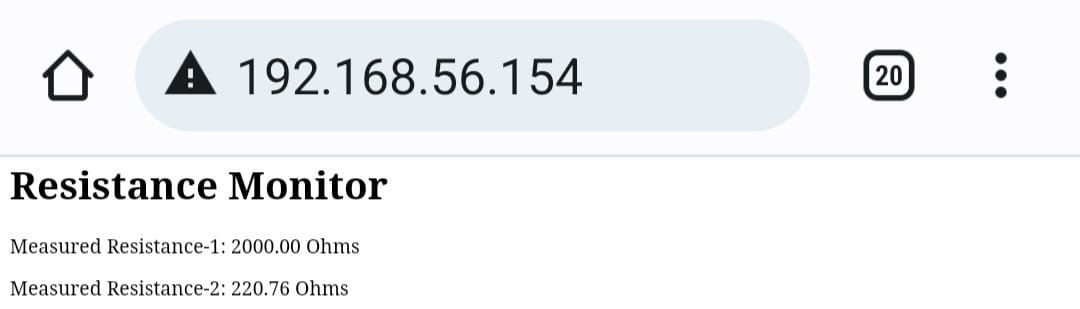
\includegraphics[width=\columnwidth]{vaman-esp32/i2c-resistance/figs/website.jpeg}
\caption{Website}
\label{fig:website_results}
\end{figure}

\section{UART Communication between Vaman-ESP32 and Arduino}
This section describes how to communicate between Vaman-ESP32 and Arduino UNO 
through UART Protocol. The Unknown resistance is measured using Arduino and 
sending the value to Vaman through UART and displaying the unknown resistance on
ESP32 Webserver.
\subsection{Components}
\begin{table}[!ht]
\centering
%%%%%%%%%%%%%%%%%%%%%%%%%%%%%%%%%%%%%%%%%%%%%%%%%%%%%%%%%%%%%%%%%%%%%%
%%                                                                  %%
%%  This is the header of a LaTeX2e file exported from Gnumeric.    %%
%%                                                                  %%
%%  This file can be compiled as it stands or included in another   %%
%%  LaTeX document. The table is based on the longtable package so  %%
%%  the longtable options (headers, footers...) can be set in the   %%
%%  preamble section below (see PRAMBLE).                           %%
%%                                                                  %%
%%  To include the file in another, the following two lines must be %%
%%  in the including file:                                          %%
%%        \def\inputGnumericTable{}                                 %%
%%  at the beginning of the file and:                               %%
%%        \input{name-of-this-file.tex}                             %%
%%  where the table is to be placed. Note also that the including   %%
%%  file must use the following packages for the table to be        %%
%%  rendered correctly:                                             %%
%%    \usepackage[latin1]{inputenc}                                 %%
%%    \usepackage{color}                                            %%
%%    \usepackage{array}                                            %%
%%    \usepackage{longtable}                                        %%
%%    \usepackage{calc}                                             %%
%%    \usepackage{multirow}                                         %%
%%    \usepackage{hhline}                                           %%
%%    \usepackage{ifthen}                                           %%
%%  optionally (for landscape tables embedded in another document): %%
%%    \usepackage{lscape}                                           %%
%%                                                                  %%
%%%%%%%%%%%%%%%%%%%%%%%%%%%%%%%%%%%%%%%%%%%%%%%%%%%%%%%%%%%%%%%%%%%%%%



%%  This section checks if we are begin input into another file or  %%
%%  the file will be compiled alone. First use a macro taken from   %%
%%  the TeXbook ex 7.7 (suggestion of Han-Wen Nienhuys).            %%
\def\ifundefined#1{\expandafter\ifx\csname#1\endcsname\relax}


%%  Check for the \def token for inputed files. If it is not        %%
%%  defined, the file will be processed as a standalone and the     %%
%%  preamble will be used.                                          %%
\ifundefined{inputGnumericTable}

%%  We must be able to close or not the document at the end.        %%
	\def\gnumericTableEnd{\end{document}}


%%%%%%%%%%%%%%%%%%%%%%%%%%%%%%%%%%%%%%%%%%%%%%%%%%%%%%%%%%%%%%%%%%%%%%
%%                                                                  %%
%%  This is the PREAMBLE. Change these values to get the right      %%
%%  paper size and other niceties.                                  %%
%%                                                                  %%
%%%%%%%%%%%%%%%%%%%%%%%%%%%%%%%%%%%%%%%%%%%%%%%%%%%%%%%%%%%%%%%%%%%%%%

	\documentclass[12pt%
			  %,landscape%
                    ]{report}
       \usepackage[latin1]{inputenc}
       \usepackage{fullpage}
       \usepackage{color}
       \usepackage{array}
       \usepackage{longtable}
       \usepackage{calc}
       \usepackage{multirow}
       \usepackage{hhline}
       \usepackage{ifthen}

	\begin{document}


%%  End of the preamble for the standalone. The next section is for %%
%%  documents which are included into other LaTeX2e files.          %%
\else

%%  We are not a stand alone document. For a regular table, we will %%
%%  have no preamble and only define the closing to mean nothing.   %%
    \def\gnumericTableEnd{}

%%  If we want landscape mode in an embedded document, comment out  %%
%%  the line above and uncomment the two below. The table will      %%
%%  begin on a new page and run in landscape mode.                  %%
%       \def\gnumericTableEnd{\end{landscape}}
%       \begin{landscape}


%%  End of the else clause for this file being \input.              %%
\fi

%%%%%%%%%%%%%%%%%%%%%%%%%%%%%%%%%%%%%%%%%%%%%%%%%%%%%%%%%%%%%%%%%%%%%%
%%                                                                  %%
%%  The rest is the gnumeric table, except for the closing          %%
%%  statement. Changes below will alter the table's appearance.     %%
%%                                                                  %%
%%%%%%%%%%%%%%%%%%%%%%%%%%%%%%%%%%%%%%%%%%%%%%%%%%%%%%%%%%%%%%%%%%%%%%

\providecommand{\gnumericmathit}[1]{#1} 
%%  Uncomment the next line if you would like your numbers to be in %%
%%  italics if they are italizised in the gnumeric table.           %%
%\renewcommand{\gnumericmathit}[1]{\mathit{#1}}
\providecommand{\gnumericPB}[1]%
{\let\gnumericTemp=\\#1\let\\=\gnumericTemp\hspace{0pt}}
 \ifundefined{gnumericTableWidthDefined}
        \newlength{\gnumericTableWidth}
        \newlength{\gnumericTableWidthComplete}
        \newlength{\gnumericMultiRowLength}
        \global\def\gnumericTableWidthDefined{}
 \fi
%% The following setting protects this code from babel shorthands.  %%
 \ifthenelse{\isundefined{\languageshorthands}}{}{\languageshorthands{english}}
%%  The default table format retains the relative column widths of  %%
%%  gnumeric. They can easily be changed to c, r or l. In that case %%
%%  you may want to comment out the next line and uncomment the one %%
%%  thereafter                                                      %%
\providecommand\gnumbox{\makebox[0pt]}
%%\providecommand\gnumbox[1][]{\makebox}

%% to adjust positions in multirow situations                       %%
\setlength{\bigstrutjot}{\jot}
\setlength{\extrarowheight}{\doublerulesep}

%%  The \setlongtables command keeps column widths the same across  %%
%%  pages. Simply comment out next line for varying column widths.  %%
\setlongtables

\setlength\gnumericTableWidth{%
	152pt+%
	60pt+%
	65pt+%
0pt}
\def\gumericNumCols{3}
\setlength\gnumericTableWidthComplete{\gnumericTableWidth+%
         \tabcolsep*\gumericNumCols*2+\arrayrulewidth*\gumericNumCols}
\ifthenelse{\lengthtest{\gnumericTableWidthComplete > \linewidth}}%
         {\def\gnumericScale{1*\ratio{\linewidth-%
                        \tabcolsep*\gumericNumCols*2-%
                        \arrayrulewidth*\gumericNumCols}%
{\gnumericTableWidth}}}%
{\def\gnumericScale{1}}

%%%%%%%%%%%%%%%%%%%%%%%%%%%%%%%%%%%%%%%%%%%%%%%%%%%%%%%%%%%%%%%%%%%%%%
%%                                                                  %%
%% The following are the widths of the various columns. We are      %%
%% defining them here because then they are easier to change.       %%
%% Depending on the cell formats we may use them more than once.    %%
%%                                                                  %%
%%%%%%%%%%%%%%%%%%%%%%%%%%%%%%%%%%%%%%%%%%%%%%%%%%%%%%%%%%%%%%%%%%%%%%

\ifthenelse{\isundefined{\gnumericColA}}{\newlength{\gnumericColA}}{}\settowidth{\gnumericColA}{\begin{tabular}{@{}p{152pt*\gnumericScale}@{}}x\end{tabular}}
\ifthenelse{\isundefined{\gnumericColB}}{\newlength{\gnumericColB}}{}\settowidth{\gnumericColB}{\begin{tabular}{@{}p{60pt*\gnumericScale}@{}}x\end{tabular}}
\ifthenelse{\isundefined{\gnumericColC}}{\newlength{\gnumericColC}}{}\settowidth{\gnumericColC}{\begin{tabular}{@{}p{65pt*\gnumericScale}@{}}x\end{tabular}}

\begin{longtable}[c]{%
	b{\gnumericColA}%
	b{\gnumericColB}%
	b{\gnumericColC}%
	}

%%%%%%%%%%%%%%%%%%%%%%%%%%%%%%%%%%%%%%%%%%%%%%%%%%%%%%%%%%%%%%%%%%%%%%
%%  The longtable options. (Caption, headers... see Goosens, p.124) %%
%	\caption{The Table Caption.}             \\	%
% \hline	% Across the top of the table.
%%  The rest of these options are table rows which are placed on    %%
%%  the first, last or every page. Use \multicolumn if you want.    %%

%%  Header for the first page.                                      %%
%	\multicolumn{3}{c}{The First Header} \\ \hline 
%	\multicolumn{1}{c}{colTag}	%Column 1
%	&\multicolumn{1}{c}{colTag}	%Column 2
%	&\multicolumn{1}{c}{colTag}	\\ \hline %Last column
%	\endfirsthead

%%  The running header definition.                                  %%
%	\hline
%	\multicolumn{3}{l}{\ldots\small\slshape continued} \\ \hline
%	\multicolumn{1}{c}{colTag}	%Column 1
%	&\multicolumn{1}{c}{colTag}	%Column 2
%	&\multicolumn{1}{c}{colTag}	\\ \hline %Last column
%	\endhead

%%  The running footer definition.                                  %%
%	\hline
%	\multicolumn{3}{r}{\small\slshape continued\ldots} \\
%	\endfoot

%%  The ending footer definition.                                   %%
%	\multicolumn{3}{c}{That's all folks} \\ \hline 
%	\endlastfoot
%%%%%%%%%%%%%%%%%%%%%%%%%%%%%%%%%%%%%%%%%%%%%%%%%%%%%%%%%%%%%%%%%%%%%%

\hhline{|-|-|-}
	 \multicolumn{1}{|p{\gnumericColA}|}%
	{\gnumericPB{\centering}\textbf{Component}}
	&\multicolumn{1}{p{\gnumericColB}|}%
	{\gnumericPB{\centering}\textbf{Value}}
	&\multicolumn{1}{p{\gnumericColC}|}%
	{\gnumericPB{\centering}\textbf{Quantity}}
\\
\hhline{|---|}
	 \multicolumn{1}{|p{\gnumericColA}|}%
	{\setlength{\gnumericMultiRowLength}{0pt}%
	 \addtolength{\gnumericMultiRowLength}{\gnumericColA}%
	 \multirow{2}[1]{\gnumericMultiRowLength}{\parbox{\gnumericMultiRowLength}{%
	 \gnumericPB{\centering}Resistor}}}
	&\multicolumn{1}{p{\gnumericColB}|}%
	{\gnumericPB{\centering}220 Ohm}
	&\multicolumn{1}{p{\gnumericColC}|}%
	{\gnumericPB{\centering}1}
\\
\hhline{~|--|}
	 \multicolumn{1}{|p{\gnumericColA}|}%
	{}
	&\multicolumn{1}{p{\gnumericColB}|}%
	{\gnumericPB{\centering}\gnumbox{1K}}
	&\multicolumn{1}{p{\gnumericColC}|}%
	{\gnumericPB{\centering}\gnumbox{1}}
\\
\hhline{|---|}
	 \multicolumn{1}{|p{\gnumericColA}|}%
	{\gnumericPB{\centering}Vaman}
	&\multicolumn{1}{p{\gnumericColB}|}%
	{\gnumericPB{\centering}LC}
	&\multicolumn{1}{p{\gnumericColC}|}%
	{\gnumericPB{\centering}1}
\\
\hhline{|---|}
	 \multicolumn{1}{|p{\gnumericColA}|}%
	{\gnumericPB{\centering}Arduino}
	&\multicolumn{1}{p{\gnumericColB}|}%
	{\gnumericPB{\centering}UNO}
	&\multicolumn{1}{p{\gnumericColC}|}%
	{\gnumericPB{\centering}1}
\\
\hhline{|---|}
	 \multicolumn{1}{|p{\gnumericColA}|}%
	{\gnumericPB{\centering}\gnumbox{Jumper Wires}}
	&\multicolumn{1}{p{\gnumericColB}|}%
	{}
	&\multicolumn{1}{p{\gnumericColC}|}%
	{\gnumericPB{\centering}\gnumbox{10}}
\\
\hhline{|---|}
	 \multicolumn{1}{|p{\gnumericColA}|}%
	{\gnumericPB{\centering}\gnumbox{Bread board}}
	&\multicolumn{1}{p{\gnumericColB}|}%
	{}
	&\multicolumn{1}{p{\gnumericColC}|}%
	{\gnumericPB{\centering}\gnumbox{1}}
\\
\hhline{|-|-|-|}
\end{longtable}

\ifthenelse{\isundefined{\languageshorthands}}{}{\languageshorthands{\languagename}}
\gnumericTableEnd

\caption{Components}
\label{table:uart-components}
\end{table}

\subsection{Connections}
\begin{enumerate}
\item
Connect the Vaman and Arduino as shown in \autoref{Tab:uart-Connections}.

\begin{table}[!ht]
\centering
%%%%%%%%%%%%%%%%%%%%%%%%%%%%%%%%%%%%%%%%%%%%%%%%%%%%%%%%%%%%%%%%%%%%%%
%%                                                                  %%
%%  This is the header of a LaTeX2e file exported from Gnumeric.    %%
%%                                                                  %%
%%  This file can be compiled as it stands or included in another   %%
%%  LaTeX document. The table is based on the longtable package so  %%
%%  the longtable options (headers, footers...) can be set in the   %%
%%  preamble section below (see PRAMBLE).                           %%
%%                                                                  %%
%%  To include the file in another, the following two lines must be %%
%%  in the including file:                                          %%
%%        \def\inputGnumericTable{}                                 %%
%%  at the beginning of the file and:                               %%
%%        \input{name-of-this-file.tex}                             %%
%%  where the table is to be placed. Note also that the including   %%
%%  file must use the following packages for the table to be        %%
%%  rendered correctly:                                             %%
%%    \usepackage[latin1]{inputenc}                                 %%
%%    \usepackage{color}                                            %%
%%    \usepackage{array}                                            %%
%%    \usepackage{longtable}                                        %%
%%    \usepackage{calc}                                             %%
%%    \usepackage{multirow}                                         %%
%%    \usepackage{hhline}                                           %%
%%    \usepackage{ifthen}                                           %%
%%  optionally (for landscape tables embedded in another document): %%
%%    \usepackage{lscape}                                           %%
%%                                                                  %%
%%%%%%%%%%%%%%%%%%%%%%%%%%%%%%%%%%%%%%%%%%%%%%%%%%%%%%%%%%%%%%%%%%%%%%



%%  This section checks if we are begin input into another file or  %%
%%  the file will be compiled alone. First use a macro taken from   %%
%%  the TeXbook ex 7.7 (suggestion of Han-Wen Nienhuys).            %%
\def\ifundefined#1{\expandafter\ifx\csname#1\endcsname\relax}


%%  Check for the \def token for inputed files. If it is not        %%
%%  defined, the file will be processed as a standalone and the     %%
%%  preamble will be used.                                          %%
\ifundefined{inputGnumericTable}

%%  We must be able to close or not the document at the end.        %%
	\def\gnumericTableEnd{\end{document}}


%%%%%%%%%%%%%%%%%%%%%%%%%%%%%%%%%%%%%%%%%%%%%%%%%%%%%%%%%%%%%%%%%%%%%%
%%                                                                  %%
%%  This is the PREAMBLE. Change these values to get the right      %%
%%  paper size and other niceties.                                  %%
%%                                                                  %%
%%%%%%%%%%%%%%%%%%%%%%%%%%%%%%%%%%%%%%%%%%%%%%%%%%%%%%%%%%%%%%%%%%%%%%

	\documentclass[12pt%
			  %,landscape%
                    ]{report}
       \usepackage[latin1]{inputenc}
       \usepackage{fullpage}
       \usepackage{color}
       \usepackage{array}
       \usepackage{longtable}
       \usepackage{calc}
       \usepackage{multirow}
       \usepackage{hhline}
       \usepackage{ifthen}

	\begin{document}


%%  End of the preamble for the standalone. The next section is for %%
%%  documents which are included into other LaTeX2e files.          %%
\else

%%  We are not a stand alone document. For a regular table, we will %%
%%  have no preamble and only define the closing to mean nothing.   %%
    \def\gnumericTableEnd{}

%%  If we want landscape mode in an embedded document, comment out  %%
%%  the line above and uncomment the two below. The table will      %%
%%  begin on a new page and run in landscape mode.                  %%
%       \def\gnumericTableEnd{\end{landscape}}
%       \begin{landscape}


%%  End of the else clause for this file being \input.              %%
\fi

%%%%%%%%%%%%%%%%%%%%%%%%%%%%%%%%%%%%%%%%%%%%%%%%%%%%%%%%%%%%%%%%%%%%%%
%%                                                                  %%
%%  The rest is the gnumeric table, except for the closing          %%
%%  statement. Changes below will alter the table's appearance.     %%
%%                                                                  %%
%%%%%%%%%%%%%%%%%%%%%%%%%%%%%%%%%%%%%%%%%%%%%%%%%%%%%%%%%%%%%%%%%%%%%%

\providecommand{\gnumericmathit}[1]{#1} 
%%  Uncomment the next line if you would like your numbers to be in %%
%%  italics if they are italizised in the gnumeric table.           %%
%\renewcommand{\gnumericmathit}[1]{\mathit{#1}}
\providecommand{\gnumericPB}[1]%
{\let\gnumericTemp=\\#1\let\\=\gnumericTemp\hspace{0pt}}
 \ifundefined{gnumericTableWidthDefined}
        \newlength{\gnumericTableWidth}
        \newlength{\gnumericTableWidthComplete}
        \newlength{\gnumericMultiRowLength}
        \global\def\gnumericTableWidthDefined{}
 \fi
%% The following setting protects this code from babel shorthands.  %%
 \ifthenelse{\isundefined{\languageshorthands}}{}{\languageshorthands{english}}
%%  The default table format retains the relative column widths of  %%
%%  gnumeric. They can easily be changed to c, r or l. In that case %%
%%  you may want to comment out the next line and uncomment the one %%
%%  thereafter                                                      %%
\providecommand\gnumbox{\makebox[0pt]}
%%\providecommand\gnumbox[1][]{\makebox}

%% to adjust positions in multirow situations                       %%
\setlength{\bigstrutjot}{\jot}
\setlength{\extrarowheight}{\doublerulesep}

%%  The \setlongtables command keeps column widths the same across  %%
%%  pages. Simply comment out next line for varying column widths.  %%
\setlongtables

\setlength\gnumericTableWidth{%
	152pt+%
	106pt+%
0pt}
\def\gumericNumCols{2}
\setlength\gnumericTableWidthComplete{\gnumericTableWidth+%
         \tabcolsep*\gumericNumCols*2+\arrayrulewidth*\gumericNumCols}
\ifthenelse{\lengthtest{\gnumericTableWidthComplete > \linewidth}}%
         {\def\gnumericScale{1*\ratio{\linewidth-%
                        \tabcolsep*\gumericNumCols*2-%
                        \arrayrulewidth*\gumericNumCols}%
{\gnumericTableWidth}}}%
{\def\gnumericScale{1}}

%%%%%%%%%%%%%%%%%%%%%%%%%%%%%%%%%%%%%%%%%%%%%%%%%%%%%%%%%%%%%%%%%%%%%%
%%                                                                  %%
%% The following are the widths of the various columns. We are      %%
%% defining them here because then they are easier to change.       %%
%% Depending on the cell formats we may use them more than once.    %%
%%                                                                  %%
%%%%%%%%%%%%%%%%%%%%%%%%%%%%%%%%%%%%%%%%%%%%%%%%%%%%%%%%%%%%%%%%%%%%%%

\ifthenelse{\isundefined{\gnumericColA}}{\newlength{\gnumericColA}}{}\settowidth{\gnumericColA}{\begin{tabular}{@{}p{152pt*\gnumericScale}@{}}x\end{tabular}}
\ifthenelse{\isundefined{\gnumericColB}}{\newlength{\gnumericColB}}{}\settowidth{\gnumericColB}{\begin{tabular}{@{}p{106pt*\gnumericScale}@{}}x\end{tabular}}

\begin{tabular}[c]{%
	b{\gnumericColA}%
	b{\gnumericColB}%
	}

%%%%%%%%%%%%%%%%%%%%%%%%%%%%%%%%%%%%%%%%%%%%%%%%%%%%%%%%%%%%%%%%%%%%%%
%%  The longtable options. (Caption, headers... see Goosens, p.124) %%
%	\caption{The Table Caption.}             \\	%
% \hline	% Across the top of the table.
%%  The rest of these options are table rows which are placed on    %%
%%  the first, last or every page. Use \multicolumn if you want.    %%

%%  Header for the first page.                                      %%
%	\multicolumn{2}{c}{The First Header} \\ \hline 
%	\multicolumn{1}{c}{colTag}	%Column 1
%	&\multicolumn{1}{c}{colTag}	\\ \hline %Last column
%	\endfirsthead

%%  The running header definition.                                  %%
%	\hline
%	\multicolumn{2}{l}{\ldots\small\slshape continued} \\ \hline
%	\multicolumn{1}{c}{colTag}	%Column 1
%	&\multicolumn{1}{c}{colTag}	\\ \hline %Last column
%	\endhead

%%  The running footer definition.                                  %%
%	\hline
%	\multicolumn{2}{r}{\small\slshape continued\ldots} \\
%	\endfoot

%%  The ending footer definition.                                   %%
%	\multicolumn{2}{c}{That's all folks} \\ \hline 
%	\endlastfoot
%%%%%%%%%%%%%%%%%%%%%%%%%%%%%%%%%%%%%%%%%%%%%%%%%%%%%%%%%%%%%%%%%%%%%%

\hhline{|-|-}
	 \multicolumn{1}{|p{\gnumericColA}|}%
	{\gnumericPB{\centering}\textbf{Arduino UNO}}
	&\multicolumn{1}{p{\gnumericColB}|}%
	{\gnumericPB{\centering}\textbf{Vaman-ESP}}
\\
\hhline{|--|}
	 \multicolumn{1}{|p{\gnumericColA}|}%
	{\gnumericPB{\centering}Rx( Pin-0 )}
	&\multicolumn{1}{p{\gnumericColB}|}%
	{\gnumericPB{\centering}17 (Tx)}
\\
\hhline{|--|}
	 \multicolumn{1}{|p{\gnumericColA}|}%
	{\gnumericPB{\centering}Tx ( Pin-1 )}
	&\multicolumn{1}{p{\gnumericColB}|}%
	{\gnumericPB{\centering}16 (Rx)}
\\
\hhline{|-|-|}
\end{tabular}

\ifthenelse{\isundefined{\languageshorthands}}{}{\languageshorthands{\languagename}}
\gnumericTableEnd

\caption{Connections}
\label{Tab:uart-Connections}
\end{table}
\item
The Vaman pin diagram is available in \autoref{fig:vaman-pin_sheet}.

\item Upload the following code to Arduino UNO

\begin{lstlisting}
vaman-esp32/uart/codes/UNO
\end{lstlisting}
\end{enumerate}
\subsection{Measuring the resistance}
\begin{enumerate}
\item
Connect the 5V pin of the Vaman-ESP32 to an extreme pin of the breadboard shown
in \autoref{fig:breadboard}. Let this pin be $V_{cc}$.
\item
Connect the GND pin of the Vaman-ESP32 to the opposite extreme pin of the 
breadboard.
\item
Let $R_1$ be the known resistor and $R_2$ be the unknown resistor. Connect $R_1$
and $R_2$ in series such that $R_1$ is connected to $V_{cc}$ and $R_2$ is
connected to GND. Refer to \autoref{fig:voltage_divider}.
\item
Connect the junction between the two resistors to the A0 pin on the Arduino
board.
\item
Now power the Vaman board.
\item
Execute the following code after editing the WiFi credentials
\begin{lstlisting}
vaman-esp32/uart/codes/VAMAN
\end{lstlisting}
\end{enumerate}
\subsection{Displaying the Measured resistance on website}
\begin{enumerate}
\item The unknown resistance is measured and diplayed the measured resistance on
the Vaman-ESP32 webserver.
\item After flashing the code to Vaman-ESP32, the board will be connected to the
WiFi credentials provided.
\item Now connect the same WiFi credentials to the mobile phone for accessing
the IP address, which can be accessed by 
\begin{lstlisting}
ifconfig
nmap -sn 192.168.x.x/24
\end{lstlisting}
\item Change the IP address in the second command accordingly with the IP
address provided by first command.
\item By the above commands the IP address of Vaman-ESP32 will be diplayed.
\item Now the Vaman-ESP32 will be hosting a webserver.
\item In order to access the webserver type the IP address of the Vaman-ESP32 in
the web browser.
\item In the website loaded by the IP address of Vaman-ESP32 the unknown 
resistance is displayed as shown in \autoref{fig:website}.
\end{enumerate}

This section describes how to communicate between Vaman-ESP32 and Arduino UNO
through SPI Protocol. Here the Arduino sketch for an ESP32 microcontroller that 
connects to a WiFi network and communicates with a server using the SPI 
protocol. It sends a message character by character to the server via the SPI 
interface and receives a response. The received response is stored in a JSON 
document and sent back to the server using an HTTP POST request.
\subsection{Components}
\numberwithin{equation}{enumi}
\numberwithin{figure}{enumi}
\numberwithin{table}{section}

\begin{table}[!ht]
\centering
%%%%%%%%%%%%%%%%%%%%%%%%%%%%%%%%%%%%%%%%%%%%%%%%%%%%%%%%%%%%%%%%%%%%%%
%%                                                                  %%
%%  This is the header of a LaTeX2e file exported from Gnumeric.    %%
%%                                                                  %%
%%  This file can be compiled as it stands or included in another   %%
%%  LaTeX document. The table is based on the longtable package so  %%
%%  the longtable options (headers, footers...) can be set in the   %%
%%  preamble section below (see PRAMBLE).                           %%
%%                                                                  %%
%%  To include the file in another, the following two lines must be %%
%%  in the including file:                                          %%
%%        \def\inputGnumericTable{}                                 %%
%%  at the beginning of the file and:                               %%
%%        \input{name-of-this-file.tex}                             %%
%%  where the table is to be placed. Note also that the including   %%
%%  file must use the following packages for the table to be        %%
%%  rendered correctly:                                             %%
%%    \usepackage[latin1]{inputenc}                                 %%
%%    \usepackage{color}                                            %%
%%    \usepackage{array}                                            %%
%%    \usepackage{longtable}                                        %%
%%    \usepackage{calc}                                             %%
%%    \usepackage{multirow}                                         %%
%%    \usepackage{hhline}                                           %%
%%    \usepackage{ifthen}                                           %%
%%  optionally (for landscape tables embedded in another document): %%
%%    \usepackage{lscape}                                           %%
%%                                                                  %%
%%%%%%%%%%%%%%%%%%%%%%%%%%%%%%%%%%%%%%%%%%%%%%%%%%%%%%%%%%%%%%%%%%%%%%



%%  This section checks if we are begin input into another file or  %%
%%  the file will be compiled alone. First use a macro taken from   %%
%%  the TeXbook ex 7.7 (suggestion of Han-Wen Nienhuys).            %%
\def\ifundefined#1{\expandafter\ifx\csname#1\endcsname\relax}


%%  Check for the \def token for inputed files. If it is not        %%
%%  defined, the file will be processed as a standalone and the     %%
%%  preamble will be used.                                          %%
\ifundefined{inputGnumericTable}

%%  We must be able to close or not the document at the end.        %%
	\def\gnumericTableEnd{\end{document}}


%%%%%%%%%%%%%%%%%%%%%%%%%%%%%%%%%%%%%%%%%%%%%%%%%%%%%%%%%%%%%%%%%%%%%%
%%                                                                  %%
%%  This is the PREAMBLE. Change these values to get the right      %%
%%  paper size and other niceties.                                  %%
%%                                                                  %%
%%%%%%%%%%%%%%%%%%%%%%%%%%%%%%%%%%%%%%%%%%%%%%%%%%%%%%%%%%%%%%%%%%%%%%

	\documentclass[12pt%
			  %,landscape%
                    ]{report}
       \usepackage[latin1]{inputenc}
       \usepackage{fullpage}
       \usepackage{color}
       \usepackage{array}
       \usepackage{longtable}
       \usepackage{calc}
       \usepackage{multirow}
       \usepackage{hhline}
       \usepackage{ifthen}

	\begin{document}


%%  End of the preamble for the standalone. The next section is for %%
%%  documents which are included into other LaTeX2e files.          %%
\else

%%  We are not a stand alone document. For a regular table, we will %%
%%  have no preamble and only define the closing to mean nothing.   %%
    \def\gnumericTableEnd{}

%%  If we want landscape mode in an embedded document, comment out  %%
%%  the line above and uncomment the two below. The table will      %%
%%  begin on a new page and run in landscape mode.                  %%
%       \def\gnumericTableEnd{\end{landscape}}
%       \begin{landscape}


%%  End of the else clause for this file being \input.              %%
\fi

%%%%%%%%%%%%%%%%%%%%%%%%%%%%%%%%%%%%%%%%%%%%%%%%%%%%%%%%%%%%%%%%%%%%%%
%%                                                                  %%
%%  The rest is the gnumeric table, except for the closing          %%
%%  statement. Changes below will alter the table's appearance.     %%
%%                                                                  %%
%%%%%%%%%%%%%%%%%%%%%%%%%%%%%%%%%%%%%%%%%%%%%%%%%%%%%%%%%%%%%%%%%%%%%%

\providecommand{\gnumericmathit}[1]{#1} 
%%  Uncomment the next line if you would like your numbers to be in %%
%%  italics if they are italizised in the gnumeric table.           %%
%\renewcommand{\gnumericmathit}[1]{\mathit{#1}}
\providecommand{\gnumericPB}[1]%
{\let\gnumericTemp=\\#1\let\\=\gnumericTemp\hspace{0pt}}
 \ifundefined{gnumericTableWidthDefined}
        \newlength{\gnumericTableWidth}
        \newlength{\gnumericTableWidthComplete}
        \newlength{\gnumericMultiRowLength}
        \global\def\gnumericTableWidthDefined{}
 \fi
%% The following setting protects this code from babel shorthands.  %%
 \ifthenelse{\isundefined{\languageshorthands}}{}{\languageshorthands{english}}
%%  The default table format retains the relative column widths of  %%
%%  gnumeric. They can easily be changed to c, r or l. In that case %%
%%  you may want to comment out the next line and uncomment the one %%
%%  thereafter                                                      %%
\providecommand\gnumbox{\makebox[0pt]}
%%\providecommand\gnumbox[1][]{\makebox}

%% to adjust positions in multirow situations                       %%
\setlength{\bigstrutjot}{\jot}
\setlength{\extrarowheight}{\doublerulesep}

%%  The \setlongtables command keeps column widths the same across  %%
%%  pages. Simply comment out next line for varying column widths.  %%
\setlongtables

\setlength\gnumericTableWidth{%
	152pt+%
	60pt+%
	65pt+%
0pt}
\def\gumericNumCols{3}
\setlength\gnumericTableWidthComplete{\gnumericTableWidth+%
         \tabcolsep*\gumericNumCols*2+\arrayrulewidth*\gumericNumCols}
\ifthenelse{\lengthtest{\gnumericTableWidthComplete > \linewidth}}%
         {\def\gnumericScale{1*\ratio{\linewidth-%
                        \tabcolsep*\gumericNumCols*2-%
                        \arrayrulewidth*\gumericNumCols}%
{\gnumericTableWidth}}}%
{\def\gnumericScale{1}}

%%%%%%%%%%%%%%%%%%%%%%%%%%%%%%%%%%%%%%%%%%%%%%%%%%%%%%%%%%%%%%%%%%%%%%
%%                                                                  %%
%% The following are the widths of the various columns. We are      %%
%% defining them here because then they are easier to change.       %%
%% Depending on the cell formats we may use them more than once.    %%
%%                                                                  %%
%%%%%%%%%%%%%%%%%%%%%%%%%%%%%%%%%%%%%%%%%%%%%%%%%%%%%%%%%%%%%%%%%%%%%%

\ifthenelse{\isundefined{\gnumericColA}}{\newlength{\gnumericColA}}{}\settowidth{\gnumericColA}{\begin{tabular}{@{}p{152pt*\gnumericScale}@{}}x\end{tabular}}
\ifthenelse{\isundefined{\gnumericColB}}{\newlength{\gnumericColB}}{}\settowidth{\gnumericColB}{\begin{tabular}{@{}p{60pt*\gnumericScale}@{}}x\end{tabular}}
\ifthenelse{\isundefined{\gnumericColC}}{\newlength{\gnumericColC}}{}\settowidth{\gnumericColC}{\begin{tabular}{@{}p{65pt*\gnumericScale}@{}}x\end{tabular}}

\begin{tabular}[c]{%
	b{\gnumericColA}%
	b{\gnumericColB}%
	b{\gnumericColC}%
	}

%%%%%%%%%%%%%%%%%%%%%%%%%%%%%%%%%%%%%%%%%%%%%%%%%%%%%%%%%%%%%%%%%%%%%%
%%  The longtable options. (Caption, headers... see Goosens, p.124) %%
%	\caption{The Table Caption.}             \\	%
% \hline	% Across the top of the table.
%%  The rest of these options are table rows which are placed on    %%
%%  the first, last or every page. Use \multicolumn if you want.    %%

%%  Header for the first page.                                      %%
%	\multicolumn{3}{c}{The First Header} \\ \hline 
%	\multicolumn{1}{c}{colTag}	%Column 1
%	&\multicolumn{1}{c}{colTag}	%Column 2
%	&\multicolumn{1}{c}{colTag}	\\ \hline %Last column
%	\endfirsthead

%%  The running header definition.                                  %%
%	\hline
%	\multicolumn{3}{l}{\ldots\small\slshape continued} \\ \hline
%	\multicolumn{1}{c}{colTag}	%Column 1
%	&\multicolumn{1}{c}{colTag}	%Column 2
%	&\multicolumn{1}{c}{colTag}	\\ \hline %Last column
%	\endhead

%%  The running footer definition.                                  %%
%	\hline
%	\multicolumn{3}{r}{\small\slshape continued\ldots} \\
%	\endfoot

%%  The ending footer definition.                                   %%
%	\multicolumn{3}{c}{That's all folks} \\ \hline 
%	\endlastfoot
%%%%%%%%%%%%%%%%%%%%%%%%%%%%%%%%%%%%%%%%%%%%%%%%%%%%%%%%%%%%%%%%%%%%%%

\hhline{|-|-|-}
	 \multicolumn{1}{|p{\gnumericColA}|}%
	{\gnumericPB{\centering}\textbf{Component}}
	&\multicolumn{1}{p{\gnumericColB}|}%
	{\gnumericPB{\centering}\textbf{Value}}
	&\multicolumn{1}{p{\gnumericColC}|}%
	{\gnumericPB{\centering}\textbf{Quantity}}

\\
\hhline{|---|}
	 \multicolumn{1}{|p{\gnumericColA}|}%
	{\gnumericPB{\centering}Vaman}
	&\multicolumn{1}{p{\gnumericColB}|}%
	{\gnumericPB{\centering}LC}
	&\multicolumn{1}{p{\gnumericColC}|}%
	{\gnumericPB{\centering}1}
\\
\hhline{|---|}
	 \multicolumn{1}{|p{\gnumericColA}|}%
	{\gnumericPB{\centering}Arduino}
	&\multicolumn{1}{p{\gnumericColB}|}%
	{\gnumericPB{\centering}UNO}
	&\multicolumn{1}{p{\gnumericColC}|}%
	{\gnumericPB{\centering}1}
\\
\hhline{|---|}
	 \multicolumn{1}{|p{\gnumericColA}|}%
	{\gnumericPB{\centering}\gnumbox{Jumper Wires}}
	&\multicolumn{1}{p{\gnumericColB}|}%
	{}
	&\multicolumn{1}{p{\gnumericColC}|}%
	{\gnumericPB{\centering}\gnumbox{10}}
\\
\hhline{|---|}
	 \multicolumn{1}{|p{\gnumericColA}|}%
	{\gnumericPB{\centering}\gnumbox{Bread board}}
	&\multicolumn{1}{p{\gnumericColB}|}%
	{}
	&\multicolumn{1}{p{\gnumericColC}|}%
	{\gnumericPB{\centering}\gnumbox{1}}
\\
\hhline{|-|-|-|}
\end{tabular}

\ifthenelse{\isundefined{\languageshorthands}}{}{\languageshorthands{\languagename}}
\gnumericTableEnd

\caption{Components}
\label{table:spi-components}
\end{table}

\subsection{Connections}
\begin{enumerate}[label=\thesection.\arabic*.,ref=\thesection.\theenumi]
\numberwithin{equation}{enumi}
\numberwithin{figure}{enumi}
\numberwithin{table}{enumi}

\item
Connect the Vaman and Arduino as shown Table. \ref{Tab:spi-Connections}.

\begin{table}[!ht]
\centering
%%%%%%%%%%%%%%%%%%%%%%%%%%%%%%%%%%%%%%%%%%%%%%%%%%%%%%%%%%%%%%%%%%%%%%
%%                                                                  %%
%%  This is the header of a LaTeX2e file exported from Gnumeric.    %%
%%                                                                  %%
%%  This file can be compiled as it stands or included in another   %%
%%  LaTeX document. The table is based on the longtable package so  %%
%%  the longtable options (headers, footers...) can be set in the   %%
%%  preamble section below (see PRAMBLE).                           %%
%%                                                                  %%
%%  To include the file in another, the following two lines must be %%
%%  in the including file:                                          %%
%%        \def\inputGnumericTable{}                                 %%
%%  at the beginning of the file and:                               %%
%%        \input{name-of-this-file.tex}                             %%
%%  where the table is to be placed. Note also that the including   %%
%%  file must use the following packages for the table to be        %%
%%  rendered correctly:                                             %%
%%    \usepackage[latin1]{inputenc}                                 %%
%%    \usepackage{color}                                            %%
%%    \usepackage{array}                                            %%
%%    \usepackage{longtable}                                        %%
%%    \usepackage{calc}                                             %%
%%    \usepackage{multirow}                                         %%
%%    \usepackage{hhline}                                           %%
%%    \usepackage{ifthen}                                           %%
%%  optionally (for landscape tables embedded in another document): %%
%%    \usepackage{lscape}                                           %%
%%                                                                  %%
%%%%%%%%%%%%%%%%%%%%%%%%%%%%%%%%%%%%%%%%%%%%%%%%%%%%%%%%%%%%%%%%%%%%%%



%%  This section checks if we are begin input into another file or  %%
%%  the file will be compiled alone. First use a macro taken from   %%
%%  the TeXbook ex 7.7 (suggestion of Han-Wen Nienhuys).            %%
\def\ifundefined#1{\expandafter\ifx\csname#1\endcsname\relax}


%%  Check for the \def token for inputed files. If it is not        %%
%%  defined, the file will be processed as a standalone and the     %%
%%  preamble will be used.                                          %%
\ifundefined{inputGnumericTable}

%%  We must be able to close or not the document at the end.        %%
	\def\gnumericTableEnd{\end{document}}


%%%%%%%%%%%%%%%%%%%%%%%%%%%%%%%%%%%%%%%%%%%%%%%%%%%%%%%%%%%%%%%%%%%%%%
%%                                                                  %%
%%  This is the PREAMBLE. Change these values to get the right      %%
%%  paper size and other niceties.                                  %%
%%                                                                  %%
%%%%%%%%%%%%%%%%%%%%%%%%%%%%%%%%%%%%%%%%%%%%%%%%%%%%%%%%%%%%%%%%%%%%%%

	\documentclass[12pt%
			  %,landscape%
                    ]{report}
       \usepackage[latin1]{inputenc}
       \usepackage{fullpage}
       \usepackage{color}
       \usepackage{array}
       \usepackage{longtable}
       \usepackage{calc}
       \usepackage{multirow}
       \usepackage{hhline}
       \usepackage{ifthen}

	\begin{document}


%%  End of the preamble for the standalone. The next section is for %%
%%  documents which are included into other LaTeX2e files.          %%
\else

%%  We are not a stand alone document. For a regular table, we will %%
%%  have no preamble and only define the closing to mean nothing.   %%
    \def\gnumericTableEnd{}

%%  If we want landscape mode in an embedded document, comment out  %%
%%  the line above and uncomment the two below. The table will      %%
%%  begin on a new page and run in landscape mode.                  %%
%       \def\gnumericTableEnd{\end{landscape}}
%       \begin{landscape}


%%  End of the else clause for this file being \input.              %%
\fi

%%%%%%%%%%%%%%%%%%%%%%%%%%%%%%%%%%%%%%%%%%%%%%%%%%%%%%%%%%%%%%%%%%%%%%
%%                                                                  %%
%%  The rest is the gnumeric table, except for the closing          %%
%%  statement. Changes below will alter the table's appearance.     %%
%%                                                                  %%
%%%%%%%%%%%%%%%%%%%%%%%%%%%%%%%%%%%%%%%%%%%%%%%%%%%%%%%%%%%%%%%%%%%%%%

\providecommand{\gnumericmathit}[1]{#1} 
%%  Uncomment the next line if you would like your numbers to be in %%
%%  italics if they are italizised in the gnumeric table.           %%
%\renewcommand{\gnumericmathit}[1]{\mathit{#1}}
\providecommand{\gnumericPB}[1]%
{\let\gnumericTemp=\\#1\let\\=\gnumericTemp\hspace{0pt}}
 \ifundefined{gnumericTableWidthDefined}
        \newlength{\gnumericTableWidth}
        \newlength{\gnumericTableWidthComplete}
        \newlength{\gnumericMultiRowLength}
        \global\def\gnumericTableWidthDefined{}
 \fi
%% The following setting protects this code from babel shorthands.  %%
 \ifthenelse{\isundefined{\languageshorthands}}{}{\languageshorthands{english}}
%%  The default table format retains the relative column widths of  %%
%%  gnumeric. They can easily be changed to c, r or l. In that case %%
%%  you may want to comment out the next line and uncomment the one %%
%%  thereafter                                                      %%
\providecommand\gnumbox{\makebox[0pt]}
%%\providecommand\gnumbox[1][]{\makebox}

%% to adjust positions in multirow situations                       %%
\setlength{\bigstrutjot}{\jot}
\setlength{\extrarowheight}{\doublerulesep}

%%  The \setlongtables command keeps column widths the same across  %%
%%  pages. Simply comment out next line for varying column widths.  %%
\setlongtables

\setlength\gnumericTableWidth{%
	65pt+%
	92pt+%
	75pt+%
0pt}
\def\gumericNumCols{3}
\setlength\gnumericTableWidthComplete{\gnumericTableWidth+%
         \tabcolsep*\gumericNumCols*2+\arrayrulewidth*\gumericNumCols}
\ifthenelse{\lengthtest{\gnumericTableWidthComplete > \linewidth}}%
         {\def\gnumericScale{\ratio{\linewidth-%
                        \tabcolsep*\gumericNumCols*2-%
                        \arrayrulewidth*\gumericNumCols}%
{\gnumericTableWidth}}}%
{\def\gnumericScale{1}}

%%%%%%%%%%%%%%%%%%%%%%%%%%%%%%%%%%%%%%%%%%%%%%%%%%%%%%%%%%%%%%%%%%%%%%
%%                                                                  %%
%% The following are the widths of the various columns. We are      %%
%% defining them here because then they are easier to change.       %%
%% Depending on the cell formats we may use them more than once.    %%
%%                                                                  %%
%%%%%%%%%%%%%%%%%%%%%%%%%%%%%%%%%%%%%%%%%%%%%%%%%%%%%%%%%%%%%%%%%%%%%%

\ifthenelse{\isundefined{\gnumericColA}}{\newlength{\gnumericColA}}{}\settowidth{\gnumericColA}{\begin{tabular}{@{}p{65pt*\gnumericScale}@{}}x\end{tabular}}
\ifthenelse{\isundefined{\gnumericColB}}{\newlength{\gnumericColB}}{}\settowidth{\gnumericColB}{\begin{tabular}{@{}p{92pt*\gnumericScale}@{}}x\end{tabular}}
\ifthenelse{\isundefined{\gnumericColC}}{\newlength{\gnumericColC}}{}\settowidth{\gnumericColC}{\begin{tabular}{@{}p{75pt*\gnumericScale}@{}}x\end{tabular}}

\begin{longtable}[c]{%
	b{\gnumericColA}%
	b{\gnumericColB}%
	b{\gnumericColC}%
	}

%%%%%%%%%%%%%%%%%%%%%%%%%%%%%%%%%%%%%%%%%%%%%%%%%%%%%%%%%%%%%%%%%%%%%%
%%  The longtable options. (Caption, headers... see Goosens, p.124) %%
%	\caption{The Table Caption.}             \\	%
% \hline	% Across the top of the table.
%%  The rest of these options are table rows which are placed on    %%
%%  the first, last or every page. Use \multicolumn if you want.    %%

%%  Header for the first page.                                      %%
%	\multicolumn{3}{c}{The First Header} \\ \hline 
%	\multicolumn{1}{c}{colTag}	%Column 1
%	&\multicolumn{1}{c}{colTag}	%Column 2
%	&\multicolumn{1}{c}{colTag}	\\ \hline %Last column
%	\endfirsthead

%%  The running header definition.                                  %%
%	\hline
%	\multicolumn{3}{l}{\ldots\small\slshape continued} \\ \hline
%	\multicolumn{1}{c}{colTag}	%Column 1
%	&\multicolumn{1}{c}{colTag}	%Column 2
%	&\multicolumn{1}{c}{colTag}	\\ \hline %Last column
%	\endhead

%%  The running footer definition.                                  %%
%	\hline
%	\multicolumn{3}{r}{\small\slshape continued\ldots} \\
%	\endfoot

%%  The ending footer definition.                                   %%
%	\multicolumn{3}{c}{That's all folks} \\ \hline 
%	\endlastfoot
%%%%%%%%%%%%%%%%%%%%%%%%%%%%%%%%%%%%%%%%%%%%%%%%%%%%%%%%%%%%%%%%%%%%%%

\hhline{|-|-|-}
	 \multicolumn{1}{|p{\gnumericColA}|}%
	{\gnumericPB{\centering}\textbf{PIN ID}}
	&\multicolumn{1}{p{\gnumericColB}|}%
	{\gnumericPB{\centering}\textbf{Vaman-ESP}}
	&\multicolumn{1}{p{\gnumericColC}|}%
	{\gnumericPB{\centering}\textbf{Ardunio}}
\\
\hhline{|---|}
	 \multicolumn{1}{|p{\gnumericColA}|}%
	{\gnumericPB{\raggedright}\gnumbox[l]{CLK}}
	&\multicolumn{1}{p{\gnumericColB}|}%
	{\gnumericPB{\raggedleft}\gnumbox[r]{14 $\hspace{1cm}$}}
	&\multicolumn{1}{p{\gnumericColC}|}%
	{\gnumericPB{\raggedright}\gnumbox[l]{$\hspace{0.5cm}$D13}}
\\
\hhline{|---|}
	 \multicolumn{1}{|p{\gnumericColA}|}%
	{\gnumericPB{\raggedright}\gnumbox[l]{MISO/CIPO}}
	&\multicolumn{1}{p{\gnumericColB}|}%
	{\gnumericPB{\raggedleft}\gnumbox[r]{12 $\hspace{1cm}$}}
	&\multicolumn{1}{p{\gnumericColC}|}%
	{\gnumericPB{\raggedright}\gnumbox[l]{$\hspace{0.5cm}$D12}}
\\
\hhline{|---|}
	 \multicolumn{1}{|p{\gnumericColA}|}%
	{\gnumericPB{\raggedright}\gnumbox[l]{MOSI/CIPO}}
	&\multicolumn{1}{p{\gnumericColB}|}%
	{\gnumericPB{\raggedleft}\gnumbox[r]{13 $\hspace{1cm}$}}
	&\multicolumn{1}{p{\gnumericColC}|}%
	{\gnumericPB{\raggedright}\gnumbox[l]{$\hspace{0.5cm}$D11}}
\\
\hhline{|---|}
	 \multicolumn{1}{|p{\gnumericColA}|}%
	{\gnumericPB{\raggedright}\gnumbox[l]{SS/CS}}
	&\multicolumn{1}{p{\gnumericColB}|}%
	{\gnumericPB{\raggedleft}\gnumbox[r]{15 $\hspace{1cm}$}}
	&\multicolumn{1}{p{\gnumericColC}|}%
	{\gnumericPB{\raggedright}\gnumbox[l]{$\hspace{0.5cm}$D10}}
\\
\hhline{|---|}
	 \multicolumn{1}{|p{\gnumericColA}|}%
	{\gnumericPB{\raggedright}\gnumbox[l]{GND}}
	&\multicolumn{1}{p{\gnumericColB}|}%
	{\gnumericPB{\raggedright}\gnumbox[l]{$\hspace{1.2cm}$GND}}
	&\multicolumn{1}{p{\gnumericColC}|}%
	{\gnumericPB{\raggedright}\gnumbox[l]{ $\hspace{0.5cm}$GND}}
\\
\hhline{|-|-|-|}
\end{longtable}

\ifthenelse{\isundefined{\languageshorthands}}{}{\languageshorthands{\languagename}}
\gnumericTableEnd

\caption{Connections}
\label{Tab:spi-Connections}
\end{table}
\item The Vaman pin diagram is available in Fig. \ref{fig:vaman-pin_sheet}

\item Upload the following code to Arduino UNO.

\begin{lstlisting}
vaman-esp32/spi/codes/arduino
pio run -t upload
\end{lstlisting}

\item Execute the following code after editing the WiFi credentials
\begin{lstlisting}
vaman-esp32/spi/codes/esp32
pio run -t upload 
\end{lstlisting}

\item To run the server, you require a Python 3 virtual environment with Flask
installed. You can run it by entering the following commands at a terminal
window
\begin{lstlisting}
vaman-esp32/spi/codes
python3 -m venv venv
source venv/bin/activate
cd ./server
ifconfig
flask run --host 192.168.xxx.xxx
\end{lstlisting}
\item Inorder to access the webserver, type the IP address of the Vaman-ESP32 in
the web browser.
\item In the website loaded by the IP address of Vaman-ESP32 is to establish a 
WiFi connection, exchange data with a server using the SPI protocol, handle 
received data, and communicate with the server using HTTP requests as shown in 
Fig. \ref{fig:results}.
\begin{figure}[!ht]
\centering
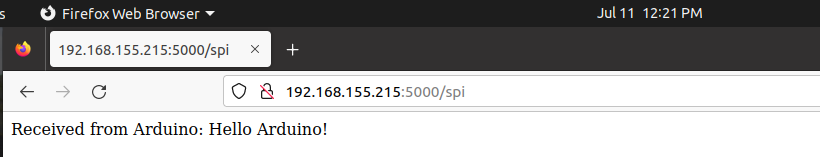
\includegraphics[width=\columnwidth]{vaman-esp32/spi/figs/result.png}
\caption{Website}
\label{fig:results}
\end{figure}
\end{enumerate}

\section{Measuring Unknown Resistance Using SPI}
This section describes how to setup the Vaman-ESP32 as a Master and  arduinos as a Slave using SPI protocol. The  unknown resistance are measured by using Arduino and sending those  resistance value to Vaman through SPI and displaying the unkwnown Resistance on ESP-Webserver.
\subsection{Components}
\begin{table}[!ht]
\centering
%%%%%%%%%%%%%%%%%%%%%%%%%%%%%%%%%%%%%%%%%%%%%%%%%%%%%%%%%%%%%%%%%%%%%%
%%                                                                  %%
%%  This is the header of a LaTeX2e file exported from Gnumeric.    %%
%%                                                                  %%
%%  This file can be compiled as it stands or included in another   %%
%%  LaTeX document. The table is based on the longtable package so  %%
%%  the longtable options (headers, footers...) can be set in the   %%
%%  preamble section below (see PRAMBLE).                           %%
%%                                                                  %%
%%  To include the file in another, the following two lines must be %%
%%  in the including file:                                          %%
%%        \def\inputGnumericTable{}                                 %%
%%  at the beginning of the file and:                               %%
%%        \input{name-of-this-file.tex}                             %%
%%  where the table is to be placed. Note also that the including   %%
%%  file must use the following packages for the table to be        %%
%%  rendered correctly:                                             %%
%%    \usepackage[latin1]{inputenc}                                 %%
%%    \usepackage{color}                                            %%
%%    \usepackage{array}                                            %%
%%    \usepackage{longtable}                                        %%
%%    \usepackage{calc}                                             %%
%%    \usepackage{multirow}                                         %%
%%    \usepackage{hhline}                                           %%
%%    \usepackage{ifthen}                                           %%
%%  optionally (for landscape tables embedded in another document): %%
%%    \usepackage{lscape}                                           %%
%%                                                                  %%
%%%%%%%%%%%%%%%%%%%%%%%%%%%%%%%%%%%%%%%%%%%%%%%%%%%%%%%%%%%%%%%%%%%%%%



%%  This section checks if we are begin input into another file or  %%
%%  the file will be compiled alone. First use a macro taken from   %%
%%  the TeXbook ex 7.7 (suggestion of Han-Wen Nienhuys).            %%
\def\ifundefined#1{\expandafter\ifx\csname#1\endcsname\relax}


%%  Check for the \def token for inputed files. If it is not        %%
%%  defined, the file will be processed as a standalone and the     %%
%%  preamble will be used.                                          %%
\ifundefined{inputGnumericTable}

%%  We must be able to close or not the document at the end.        %%
	\def\gnumericTableEnd{\end{document}}


%%%%%%%%%%%%%%%%%%%%%%%%%%%%%%%%%%%%%%%%%%%%%%%%%%%%%%%%%%%%%%%%%%%%%%
%%                                                                  %%
%%  This is the PREAMBLE. Change these values to get the right      %%
%%  paper size and other niceties.                                  %%
%%                                                                  %%
%%%%%%%%%%%%%%%%%%%%%%%%%%%%%%%%%%%%%%%%%%%%%%%%%%%%%%%%%%%%%%%%%%%%%%

	\documentclass[12pt%
			  %,landscape%
                    ]{report}
       \usepackage[latin1]{inputenc}
       \usepackage{fullpage}
       \usepackage{color}
       \usepackage{array}
       \usepackage{longtable}
       \usepackage{calc}
       \usepackage{multirow}
       \usepackage{hhline}
       \usepackage{ifthen}

	\begin{document}


%%  End of the preamble for the standalone. The next section is for %%
%%  documents which are included into other LaTeX2e files.          %%
\else

%%  We are not a stand alone document. For a regular table, we will %%
%%  have no preamble and only define the closing to mean nothing.   %%
    \def\gnumericTableEnd{}

%%  If we want landscape mode in an embedded document, comment out  %%
%%  the line above and uncomment the two below. The table will      %%
%%  begin on a new page and run in landscape mode.                  %%
%       \def\gnumericTableEnd{\end{landscape}}
%       \begin{landscape}


%%  End of the else clause for this file being \input.              %%
\fi

%%%%%%%%%%%%%%%%%%%%%%%%%%%%%%%%%%%%%%%%%%%%%%%%%%%%%%%%%%%%%%%%%%%%%%
%%                                                                  %%
%%  The rest is the gnumeric table, except for the closing          %%
%%  statement. Changes below will alter the table's appearance.     %%
%%                                                                  %%
%%%%%%%%%%%%%%%%%%%%%%%%%%%%%%%%%%%%%%%%%%%%%%%%%%%%%%%%%%%%%%%%%%%%%%

\providecommand{\gnumericmathit}[1]{#1} 
%%  Uncomment the next line if you would like your numbers to be in %%
%%  italics if they are italizised in the gnumeric table.           %%
%\renewcommand{\gnumericmathit}[1]{\mathit{#1}}
\providecommand{\gnumericPB}[1]%
{\let\gnumericTemp=\\#1\let\\=\gnumericTemp\hspace{0pt}}
 \ifundefined{gnumericTableWidthDefined}
        \newlength{\gnumericTableWidth}
        \newlength{\gnumericTableWidthComplete}
        \newlength{\gnumericMultiRowLength}
        \global\def\gnumericTableWidthDefined{}
 \fi
%% The following setting protects this code from babel shorthands.  %%
 \ifthenelse{\isundefined{\languageshorthands}}{}{\languageshorthands{english}}
%%  The default table format retains the relative column widths of  %%
%%  gnumeric. They can easily be changed to c, r or l. In that case %%
%%  you may want to comment out the next line and uncomment the one %%
%%  thereafter                                                      %%
\providecommand\gnumbox{\makebox[0pt]}
%%\providecommand\gnumbox[1][]{\makebox}

%% to adjust positions in multirow situations                       %%
\setlength{\bigstrutjot}{\jot}
\setlength{\extrarowheight}{\doublerulesep}

%%  The \setlongtables command keeps column widths the same across  %%
%%  pages. Simply comment out next line for varying column widths.  %%
\setlongtables

\setlength\gnumericTableWidth{%
	152pt+%
	60pt+%
	65pt+%
0pt}
\def\gumericNumCols{3}
\setlength\gnumericTableWidthComplete{\gnumericTableWidth+%
         \tabcolsep*\gumericNumCols*2+\arrayrulewidth*\gumericNumCols}
\ifthenelse{\lengthtest{\gnumericTableWidthComplete > \linewidth}}%
         {\def\gnumericScale{1*\ratio{\linewidth-%
                        \tabcolsep*\gumericNumCols*2-%
                        \arrayrulewidth*\gumericNumCols}%
{\gnumericTableWidth}}}%
{\def\gnumericScale{1}}

%%%%%%%%%%%%%%%%%%%%%%%%%%%%%%%%%%%%%%%%%%%%%%%%%%%%%%%%%%%%%%%%%%%%%%
%%                                                                  %%
%% The following are the widths of the various columns. We are      %%
%% defining them here because then they are easier to change.       %%
%% Depending on the cell formats we may use them more than once.    %%
%%                                                                  %%
%%%%%%%%%%%%%%%%%%%%%%%%%%%%%%%%%%%%%%%%%%%%%%%%%%%%%%%%%%%%%%%%%%%%%%

\ifthenelse{\isundefined{\gnumericColA}}{\newlength{\gnumericColA}}{}\settowidth{\gnumericColA}{\begin{tabular}{@{}p{152pt*\gnumericScale}@{}}x\end{tabular}}
\ifthenelse{\isundefined{\gnumericColB}}{\newlength{\gnumericColB}}{}\settowidth{\gnumericColB}{\begin{tabular}{@{}p{60pt*\gnumericScale}@{}}x\end{tabular}}
\ifthenelse{\isundefined{\gnumericColC}}{\newlength{\gnumericColC}}{}\settowidth{\gnumericColC}{\begin{tabular}{@{}p{65pt*\gnumericScale}@{}}x\end{tabular}}

\begin{longtable}[c]{%
	b{\gnumericColA}%
	b{\gnumericColB}%
	b{\gnumericColC}%
	}

%%%%%%%%%%%%%%%%%%%%%%%%%%%%%%%%%%%%%%%%%%%%%%%%%%%%%%%%%%%%%%%%%%%%%%
%%  The longtable options. (Caption, headers... see Goosens, p.124) %%
%	\caption{The Table Caption.}             \\	%
% \hline	% Across the top of the table.
%%  The rest of these options are table rows which are placed on    %%
%%  the first, last or every page. Use \multicolumn if you want.    %%

%%  Header for the first page.                                      %%
%	\multicolumn{3}{c}{The First Header} \\ \hline 
%	\multicolumn{1}{c}{colTag}	%Column 1
%	&\multicolumn{1}{c}{colTag}	%Column 2
%	&\multicolumn{1}{c}{colTag}	\\ \hline %Last column
%	\endfirsthead

%%  The running header definition.                                  %%
%	\hline
%	\multicolumn{3}{l}{\ldots\small\slshape continued} \\ \hline
%	\multicolumn{1}{c}{colTag}	%Column 1
%	&\multicolumn{1}{c}{colTag}	%Column 2
%	&\multicolumn{1}{c}{colTag}	\\ \hline %Last column
%	\endhead

%%  The running footer definition.                                  %%
%	\hline
%	\multicolumn{3}{r}{\small\slshape continued\ldots} \\
%	\endfoot

%%  The ending footer definition.                                   %%
%	\multicolumn{3}{c}{That's all folks} \\ \hline 
%	\endlastfoot
%%%%%%%%%%%%%%%%%%%%%%%%%%%%%%%%%%%%%%%%%%%%%%%%%%%%%%%%%%%%%%%%%%%%%%

\hhline{|-|-|-}
	 \multicolumn{1}{|p{\gnumericColA}|}%
	{\gnumericPB{\centering}\textbf{Component}}
	&\multicolumn{1}{p{\gnumericColB}|}%
	{\gnumericPB{\centering}\textbf{Value}}
	&\multicolumn{1}{p{\gnumericColC}|}%
	{\gnumericPB{\centering}\textbf{Quantity}}
\\
\hhline{|---|}
	 \multicolumn{1}{|p{\gnumericColA}|}%
	{\setlength{\gnumericMultiRowLength}{0pt}%
	 \addtolength{\gnumericMultiRowLength}{\gnumericColA}%
	 \multirow{2}[1]{\gnumericMultiRowLength}{\parbox{\gnumericMultiRowLength}{%
	 \gnumericPB{\centering}Resistor}}}
	&\multicolumn{1}{p{\gnumericColB}|}%
	{\gnumericPB{\centering}unknown  Ohm}
	&\multicolumn{1}{p{\gnumericColC}|}%
	{\gnumericPB{\centering}1}
\\
\hhline{~|--|}
	 \multicolumn{1}{|p{\gnumericColA}|}%
	{}
	&\multicolumn{1}{p{\gnumericColB}|}%
	{\gnumericPB{\centering}\gnumbox{1K}}
	&\multicolumn{1}{p{\gnumericColC}|}%
	{\gnumericPB{\centering}\gnumbox{1}}
\\
\hhline{|---|}
	 \multicolumn{1}{|p{\gnumericColA}|}%
	{\gnumericPB{\centering}Vaman}
	&\multicolumn{1}{p{\gnumericColB}|}%
	{\gnumericPB{\centering}LC}
	&\multicolumn{1}{p{\gnumericColC}|}%
	{\gnumericPB{\centering}1}
\\
\hhline{|---|}
	 \multicolumn{1}{|p{\gnumericColA}|}%
	{\gnumericPB{\centering}Arduino}
	&\multicolumn{1}{p{\gnumericColB}|}%
	{\gnumericPB{\centering}UNO}
	&\multicolumn{1}{p{\gnumericColC}|}%
	{\gnumericPB{\centering}1}
\\
\hhline{|---|}
	 \multicolumn{1}{|p{\gnumericColA}|}%
	{\gnumericPB{\centering}\gnumbox{Jumper Wires}}
	&\multicolumn{1}{p{\gnumericColB}|}%
	{}
	&\multicolumn{1}{p{\gnumericColC}|}%
	{\gnumericPB{\centering}\gnumbox{10}}
\\
\hhline{|---|}
	 \multicolumn{1}{|p{\gnumericColA}|}%
	{\gnumericPB{\centering}\gnumbox{Bread board}}
	&\multicolumn{1}{p{\gnumericColB}|}%
	{}
	&\multicolumn{1}{p{\gnumericColC}|}%
	{\gnumericPB{\centering}\gnumbox{1}}
\\
\hhline{|-|-|-|}
\end{longtable}

\ifthenelse{\isundefined{\languageshorthands}}{}{\languageshorthands{\languagename}}
\gnumericTableEnd

\caption{Components}
\label{table:SPI-components}
\end{table}

\subsection{Connections}
\begin{enumerate}
\item
Connect the Vaman and Arduino as shown \autoref{Tab:SPI-Connection}.

\begin{table}[!ht]
\centering
%%%%%%%%%%%%%%%%%%%%%%%%%%%%%%%%%%%%%%%%%%%%%%%%%%%%%%%%%%%%%%%%%%%%%%
%%                                                                  %%
%%  This is the header of a LaTeX2e file exported from Gnumeric.    %%
%%                                                                  %%
%%  This file can be compiled as it stands or included in another   %%
%%  LaTeX document. The table is based on the longtable package so  %%
%%  the longtable options (headers, footers...) can be set in the   %%
%%  preamble section below (see PRAMBLE).                           %%
%%                                                                  %%
%%  To include the file in another, the following two lines must be %%
%%  in the including file:                                          %%
%%        \def\inputGnumericTable{}                                 %%
%%  at the beginning of the file and:                               %%
%%        \input{name-of-this-file.tex}                             %%
%%  where the table is to be placed. Note also that the including   %%
%%  file must use the following packages for the table to be        %%
%%  rendered correctly:                                             %%
%%    \usepackage[latin1]{inputenc}                                 %%
%%    \usepackage{color}                                            %%
%%    \usepackage{array}                                            %%
%%    \usepackage{longtable}                                        %%
%%    \usepackage{calc}                                             %%
%%    \usepackage{multirow}                                         %%
%%    \usepackage{hhline}                                           %%
%%    \usepackage{ifthen}                                           %%
%%  optionally (for landscape tables embedded in another document): %%
%%    \usepackage{lscape}                                           %%
%%                                                                  %%
%%%%%%%%%%%%%%%%%%%%%%%%%%%%%%%%%%%%%%%%%%%%%%%%%%%%%%%%%%%%%%%%%%%%%%



%%  This section checks if we are begin input into another file or  %%
%%  the file will be compiled alone. First use a macro taken from   %%
%%  the TeXbook ex 7.7 (suggestion of Han-Wen Nienhuys).            %%
\def\ifundefined#1{\expandafter\ifx\csname#1\endcsname\relax}


%%  Check for the \def token for inputed files. If it is not        %%
%%  defined, the file will be processed as a standalone and the     %%
%%  preamble will be used.                                          %%
\ifundefined{inputGnumericTable}

%%  We must be able to close or not the document at the end.        %%
	\def\gnumericTableEnd{\end{document}}


%%%%%%%%%%%%%%%%%%%%%%%%%%%%%%%%%%%%%%%%%%%%%%%%%%%%%%%%%%%%%%%%%%%%%%
%%                                                                  %%
%%  This is the PREAMBLE. Change these values to get the right      %%
%%  paper size and other niceties.                                  %%
%%                                                                  %%
%%%%%%%%%%%%%%%%%%%%%%%%%%%%%%%%%%%%%%%%%%%%%%%%%%%%%%%%%%%%%%%%%%%%%%

	\documentclass[12pt%
			  %,landscape%
                    ]{report}
       \usepackage[latin1]{inputenc}
       \usepackage{fullpage}
       \usepackage{color}
       \usepackage{array}
       \usepackage{longtable}
       \usepackage{calc}
       \usepackage{multirow}
       \usepackage{hhline}
       \usepackage{ifthen}

	\begin{document}


%%  End of the preamble for the standalone. The next section is for %%
%%  documents which are included into other LaTeX2e files.          %%
\else

%%  We are not a stand alone document. For a regular table, we will %%
%%  have no preamble and only define the closing to mean nothing.   %%
    \def\gnumericTableEnd{}

%%  If we want landscape mode in an embedded document, comment out  %%
%%  the line above and uncomment the two below. The table will      %%
%%  begin on a new page and run in landscape mode.                  %%
%       \def\gnumericTableEnd{\end{landscape}}
%       \begin{landscape}


%%  End of the else clause for this file being \input.              %%
\fi

%%%%%%%%%%%%%%%%%%%%%%%%%%%%%%%%%%%%%%%%%%%%%%%%%%%%%%%%%%%%%%%%%%%%%%
%%                                                                  %%
%%  The rest is the gnumeric table, except for the closing          %%
%%  statement. Changes below will alter the table's appearance.     %%
%%                                                                  %%
%%%%%%%%%%%%%%%%%%%%%%%%%%%%%%%%%%%%%%%%%%%%%%%%%%%%%%%%%%%%%%%%%%%%%%

\providecommand{\gnumericmathit}[1]{#1} 
%%  Uncomment the next line if you would like your numbers to be in %%
%%  italics if they are italizised in the gnumeric table.           %%
%\renewcommand{\gnumericmathit}[1]{\mathit{#1}}
\providecommand{\gnumericPB}[1]%
{\let\gnumericTemp=\\#1\let\\=\gnumericTemp\hspace{0pt}}
 \ifundefined{gnumericTableWidthDefined}
        \newlength{\gnumericTableWidth}
        \newlength{\gnumericTableWidthComplete}
        \newlength{\gnumericMultiRowLength}
        \global\def\gnumericTableWidthDefined{}
 \fi
%% The following setting protects this code from babel shorthands.  %%
 \ifthenelse{\isundefined{\languageshorthands}}{}{\languageshorthands{english}}
%%  The default table format retains the relative column widths of  %%
%%  gnumeric. They can easily be changed to c, r or l. In that case %%
%%  you may want to comment out the next line and uncomment the one %%
%%  thereafter                                                      %%
\providecommand\gnumbox{\makebox[0pt]}
%%\providecommand\gnumbox[1][]{\makebox}

%% to adjust positions in multirow situations                       %%
\setlength{\bigstrutjot}{\jot}
\setlength{\extrarowheight}{\doublerulesep}

%%  The \setlongtables command keeps column widths the same across  %%
%%  pages. Simply comment out next line for varying column widths.  %%
\setlongtables

\setlength\gnumericTableWidth{%
	152pt+%
	106pt+%
0pt}
\def\gumericNumCols{2}
\setlength\gnumericTableWidthComplete{\gnumericTableWidth+%
         \tabcolsep*\gumericNumCols*2+\arrayrulewidth*\gumericNumCols}
\ifthenelse{\lengthtest{\gnumericTableWidthComplete > \linewidth}}%
         {\def\gnumericScale{1*\ratio{\linewidth-%
                        \tabcolsep*\gumericNumCols*2-%
                        \arrayrulewidth*\gumericNumCols}%
{\gnumericTableWidth}}}%
{\def\gnumericScale{1}}

%%%%%%%%%%%%%%%%%%%%%%%%%%%%%%%%%%%%%%%%%%%%%%%%%%%%%%%%%%%%%%%%%%%%%%
%%                                                                  %%
%% The following are the widths of the various columns. We are      %%
%% defining them here because then they are easier to change.       %%
%% Depending on the cell formats we may use them more than once.    %%
%%                                                                  %%
%%%%%%%%%%%%%%%%%%%%%%%%%%%%%%%%%%%%%%%%%%%%%%%%%%%%%%%%%%%%%%%%%%%%%%

\ifthenelse{\isundefined{\gnumericColA}}{\newlength{\gnumericColA}}{}\settowidth{\gnumericColA}{\begin{tabular}{@{}p{152pt*\gnumericScale}@{}}x\end{tabular}}
\ifthenelse{\isundefined{\gnumericColB}}{\newlength{\gnumericColB}}{}\settowidth{\gnumericColB}{\begin{tabular}{@{}p{106pt*\gnumericScale}@{}}x\end{tabular}}

\begin{tabular}[c]{%
	b{\gnumericColA}%
	b{\gnumericColB}%
	}

%%%%%%%%%%%%%%%%%%%%%%%%%%%%%%%%%%%%%%%%%%%%%%%%%%%%%%%%%%%%%%%%%%%%%%
%%  The longtable options. (Caption, headers... see Goosens, p.124) %%
%	\caption{The Table Caption.}             \\	%
% \hline	% Across the top of the table.
%%  The rest of these options are table rows which are placed on    %%
%%  the first, last or every page. Use \multicolumn if you want.    %%

%%  Header for the first page.                                      %%
%	\multicolumn{2}{c}{The First Header} \\ \hline 
%	\multicolumn{1}{c}{colTag}	%Column 1
%	&\multicolumn{1}{c}{colTag}	\\ \hline %Last column
%	\endfirsthead

%%  The running header definition.                                  %%
%	\hline
%	\multicolumn{2}{l}{\ldots\small\slshape continued} \\ \hline
%	\multicolumn{1}{c}{colTag}	%Column 1
%	&\multicolumn{1}{c}{colTag}	\\ \hline %Last column
%	\endhead

%%  The running footer definition.                                  %%
%	\hline
%	\multicolumn{2}{r}{\small\slshape continued\ldots} \\
%	\endfoot

%%  The ending footer definition.                                   %%
%	\multicolumn{2}{c}{That's all folks} \\ \hline 
%	\endlastfoot
%%%%%%%%%%%%%%%%%%%%%%%%%%%%%%%%%%%%%%%%%%%%%%%%%%%%%%%%%%%%%%%%%%%%%%

\hhline{|-|-}
	 \multicolumn{1}{|p{\gnumericColA}|}%
	{\gnumericPB{\centering}\textbf{Arduino UNO}}
	&\multicolumn{1}{p{\gnumericColB}|}%
	{\gnumericPB{\centering}\textbf{Vaman-ESP}}
\\
\hhline{|--|}
	 \multicolumn{1}{|p{\gnumericColA}|}%
	{\gnumericPB{\centering}Rx( Pin-0 )}
	&\multicolumn{1}{p{\gnumericColB}|}%
	{\gnumericPB{\centering}17 (Tx)}
\\
\hhline{|--|}
	 \multicolumn{1}{|p{\gnumericColA}|}%
	{\gnumericPB{\centering}Tx ( Pin-1 )}
	&\multicolumn{1}{p{\gnumericColB}|}%
	{\gnumericPB{\centering}16 (Rx)}
\\
\hhline{|-|-|}
\end{tabular}

\ifthenelse{\isundefined{\languageshorthands}}{}{\languageshorthands{\languagename}}
\gnumericTableEnd

\caption{Connections}
\label{Tab:SPI-Connection}
\end{table}
\item
The Vaman pin diagram is available in \autoref{fig:vaman-pin_sheet}.

\item Upload the following code to Arduino UNO.
\begin{lstlisting}
vaman-esp32/spi-resistance/codes/arduino
\end{lstlisting}
\end{enumerate}
\subsection{Measuring the resistance}
\begin{enumerate}
\item
Connect the 5V pin of the Vaman-ESP32 to an extreme pin of the breadboard shown 
in \autoref{fig:breadboard}. Let this pin be $V_{cc}$.
\item
Connect the GND pin of the Vaman-ESP32 to the opposite extreme pin of the 
breadboard.
\item
Let $R_1$ be the known resistor and $R_2$ be the unknown resistor. Connect $R_1$
and $R_2$ in series such that $R_1$ is connected to $V_{cc}$ and $R_2$ is 
connected to GND. Refer to \autoref{fig:voltage_divider}.
\item
Connect the junction between the two resistors to the A0 pin on the Vaman-ESP32 
GPIO36, which measures the unknown resistance.
\item
Now, power the Vaman board.
\item
Execute the following code after editing the WiFi credentials.
\begin{lstlisting}
vaman-esp32/spi-resistance/codes/esp32
\end{lstlisting}
\end{enumerate}
\subsection{Displaying the Measured resistance on website}
\begin{enumerate}
\item The unknown resistance is measured and diplayed the measured resistance on
the Vaman-ESP32 webserver.
\item After flashing the code to Vaman-ESP32, the board will be connected to the
WiFi credentials provided.
\item Now connect the same WiFi credentials to the mobile phone for accessing 
the IP address, which can be accessed by 
\begin{lstlisting}
ifconfig
nmap -sn 192.168.x.x/24
\end{lstlisting}
\item Change the IP address in the second command accordingly with the IP 
address provided by first command.
\item By the above commands the IP address of Vaman-ESP32 will be displayed.
\item Now the Vaman-ESP32 will be hosting a webserver.
\item In order to access the webserver type the IP address of the Vaman-ESP32 in
the web browser.
\item In the website loaded by the IP address of Vaman-ESP32, the unknown 
resistance is displayed as shown in \autoref{fig:results1}.
\begin{figure}[!ht]
\centering
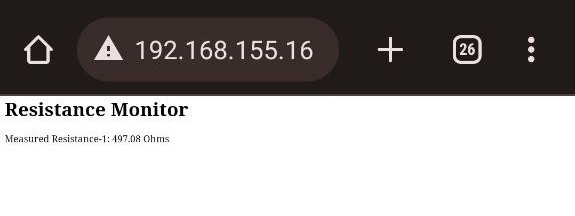
\includegraphics[width=\columnwidth]{vaman-esp32/spi-resistance/figs/result.jpg}
\caption{Website}
\label{fig:results1}
\end{figure}
\end{enumerate}

\section{Bluetooth-Controlled Seven Segment Display}
This section describes how to control the seven-segment display through the
Dabble Android application using Bluetooth, and display an appropriate digit on
the seven-segment display according to the controls in the Android app.

\subsection{Components}
\begin{table}[!ht]
\centering
%%%%%%%%%%%%%%%%%%%%%%%%%%%%%%%%%%%%%%%%%%%%%%%%%%%%%%%%%%%%%%%%%%%%%%
%%                                                                  %%
%%  This is the header of a LaTeX2e file exported from Gnumeric.    %%
%%                                                                  %%
%%  This file can be compiled as it stands or included in another   %%
%%  LaTeX document. The table is based on the longtable package so  %%
%%  the longtable options (headers, footers...) can be set in the   %%
%%  preamble section below (see PRAMBLE).                           %%
%%                                                                  %%
%%  To include the file in another, the following two lines must be %%
%%  in the including file:                                          %%
%%        \def\inputGnumericTable{}                                 %%
%%  at the beginning of the file and:                               %%
%%        \input{name-of-this-file.tex}                             %%
%%  where the table is to be placed. Note also that the including   %%
%%  file must use the following packages for the table to be        %%
%%  rendered correctly:                                             %%
%%    \usepackage[latin1]{inputenc}                                 %%
%%    \usepackage{color}                                            %%
%%    \usepackage{array}                                            %%
%%    \usepackage{longtable}                                        %%
%%    \usepackage{calc}                                             %%
%%    \usepackage{multirow}                                         %%
%%    \usepackage{hhline}                                           %%
%%    \usepackage{ifthen}                                           %%
%%  optionally (for landscape tables embedded in another document): %%
%%    \usepackage{lscape}                                           %%
%%                                                                  %%
%%%%%%%%%%%%%%%%%%%%%%%%%%%%%%%%%%%%%%%%%%%%%%%%%%%%%%%%%%%%%%%%%%%%%%



%%  This section checks if we are begin input into another file or  %%
%%  the file will be compiled alone. First use a macro taken from   %%
%%  the TeXbook ex 7.7 (suggestion of Han-Wen Nienhuys).            %%
\def\ifundefined#1{\expandafter\ifx\csname#1\endcsname\relax}


%%  Check for the \def token for inputed files. If it is not        %%
%%  defined, the file will be processed as a standalone and the     %%
%%  preamble will be used.                                          %%
\ifundefined{inputGnumericTable}

%%  We must be able to close or not the document at the end.        %%
	\def\gnumericTableEnd{\end{document}}


%%%%%%%%%%%%%%%%%%%%%%%%%%%%%%%%%%%%%%%%%%%%%%%%%%%%%%%%%%%%%%%%%%%%%%
%%                                                                  %%
%%  This is the PREAMBLE. Change these values to get the right      %%
%%  paper size and other niceties.                                  %%
%%                                                                  %%
%%%%%%%%%%%%%%%%%%%%%%%%%%%%%%%%%%%%%%%%%%%%%%%%%%%%%%%%%%%%%%%%%%%%%%

	\documentclass[12pt%
			  %,landscape%
                    ]{report}
       \usepackage[latin1]{inputenc}
       \usepackage{fullpage}
       \usepackage{color}
       \usepackage{array}
       \usepackage{longtable}
       \usepackage{calc}
       \usepackage{multirow}
       \usepackage{hhline}
       \usepackage{ifthen}

	\begin{document}


%%  End of the preamble for the standalone. The next section is for %%
%%  documents which are included into other LaTeX2e files.          %%
\else

%%  We are not a stand alone document. For a regular table, we will %%
%%  have no preamble and only define the closing to mean nothing.   %%
    \def\gnumericTableEnd{}

%%  If we want landscape mode in an embedded document, comment out  %%
%%  the line above and uncomment the two below. The table will      %%
%%  begin on a new page and run in landscape mode.                  %%
%       \def\gnumericTableEnd{\end{landscape}}
%       \begin{landscape}


%%  End of the else clause for this file being \input.              %%
\fi

%%%%%%%%%%%%%%%%%%%%%%%%%%%%%%%%%%%%%%%%%%%%%%%%%%%%%%%%%%%%%%%%%%%%%%
%%                                                                  %%
%%  The rest is the gnumeric table, except for the closing          %%
%%  statement. Changes below will alter the table's appearance.     %%
%%                                                                  %%
%%%%%%%%%%%%%%%%%%%%%%%%%%%%%%%%%%%%%%%%%%%%%%%%%%%%%%%%%%%%%%%%%%%%%%

\providecommand{\gnumericmathit}[1]{#1} 
%%  Uncomment the next line if you would like your numbers to be in %%
%%  italics if they are italizised in the gnumeric table.           %%
%\renewcommand{\gnumericmathit}[1]{\mathit{#1}}
\providecommand{\gnumericPB}[1]%
{\let\gnumericTemp=\\#1\let\\=\gnumericTemp\hspace{0pt}}
 \ifundefined{gnumericTableWidthDefined}
        \newlength{\gnumericTableWidth}
        \newlength{\gnumericTableWidthComplete}
        \newlength{\gnumericMultiRowLength}
        \global\def\gnumericTableWidthDefined{}
 \fi
%% The following setting protects this code from babel shorthands.  %%
 \ifthenelse{\isundefined{\languageshorthands}}{}{\languageshorthands{english}}
%%  The default table format retains the relative column widths of  %%
%%  gnumeric. They can easily be changed to c, r or l. In that case %%
%%  you may want to comment out the next line and uncomment the one %%
%%  thereafter                                                      %%
\providecommand\gnumbox{\makebox[0pt]}
%%\providecommand\gnumbox[1][]{\makebox}

%% to adjust positions in multirow situations                       %%
\setlength{\bigstrutjot}{\jot}
\setlength{\extrarowheight}{\doublerulesep}

%%  The \setlongtables command keeps column widths the same across  %%
%%  pages. Simply comment out next line for varying column widths.  %%
\setlongtables

\setlength\gnumericTableWidth{%
	152pt+%
	60pt+%
	65pt+%
0pt}
\def\gumericNumCols{3}
\setlength\gnumericTableWidthComplete{\gnumericTableWidth+%
         \tabcolsep*\gumericNumCols*2+\arrayrulewidth*\gumericNumCols}
\ifthenelse{\lengthtest{\gnumericTableWidthComplete > \linewidth}}%
         {\def\gnumericScale{1*\ratio{\linewidth-%
                        \tabcolsep*\gumericNumCols*2-%
                        \arrayrulewidth*\gumericNumCols}%
{\gnumericTableWidth}}}%
{\def\gnumericScale{1}}

%%%%%%%%%%%%%%%%%%%%%%%%%%%%%%%%%%%%%%%%%%%%%%%%%%%%%%%%%%%%%%%%%%%%%%
%%                                                                  %%
%% The following are the widths of the various columns. We are      %%
%% defining them here because then they are easier to change.       %%
%% Depending on the cell formats we may use them more than once.    %%
%%                                                                  %%
%%%%%%%%%%%%%%%%%%%%%%%%%%%%%%%%%%%%%%%%%%%%%%%%%%%%%%%%%%%%%%%%%%%%%%

\ifthenelse{\isundefined{\gnumericColA}}{\newlength{\gnumericColA}}{}\settowidth{\gnumericColA}{\begin{tabular}{@{}p{152pt*\gnumericScale}@{}}x\end{tabular}}
\ifthenelse{\isundefined{\gnumericColB}}{\newlength{\gnumericColB}}{}\settowidth{\gnumericColB}{\begin{tabular}{@{}p{60pt*\gnumericScale}@{}}x\end{tabular}}
\ifthenelse{\isundefined{\gnumericColC}}{\newlength{\gnumericColC}}{}\settowidth{\gnumericColC}{\begin{tabular}{@{}p{65pt*\gnumericScale}@{}}x\end{tabular}}

\begin{tabular}[c]{%
	b{\gnumericColA}%
	b{\gnumericColB}%
	b{\gnumericColC}%
	}

%%%%%%%%%%%%%%%%%%%%%%%%%%%%%%%%%%%%%%%%%%%%%%%%%%%%%%%%%%%%%%%%%%%%%%
%%  The longtable options. (Caption, headers... see Goosens, p.124) %%
%	\caption{The Table Caption.}             \\	%
% \hline	% Across the top of the table.
%%  The rest of these options are table rows which are placed on    %%
%%  the first, last or every page. Use \multicolumn if you want.    %%

%%  Header for the first page.                                      %%
%	\multicolumn{3}{c}{The First Header} \\ \hline 
%	\multicolumn{1}{c}{colTag}	%Column 1
%	&\multicolumn{1}{c}{colTag}	%Column 2
%	&\multicolumn{1}{c}{colTag}	\\ \hline %Last column
%	\endfirsthead

%%  The running header definition.                                  %%
%	\hline
%	\multicolumn{3}{l}{\ldots\small\slshape continued} \\ \hline
%	\multicolumn{1}{c}{colTag}	%Column 1
%	&\multicolumn{1}{c}{colTag}	%Column 2
%	&\multicolumn{1}{c}{colTag}	\\ \hline %Last column
%	\endhead

%%  The running footer definition.                                  %%
%	\hline
%	\multicolumn{3}{r}{\small\slshape continued\ldots} \\
%	\endfoot

%%  The ending footer definition.                                   %%
%	\multicolumn{3}{c}{That's all folks} \\ \hline 
%	\endlastfoot
%%%%%%%%%%%%%%%%%%%%%%%%%%%%%%%%%%%%%%%%%%%%%%%%%%%%%%%%%%%%%%%%%%%%%%

\hhline{|-|-|-}
	 \multicolumn{1}{|p{\gnumericColA}|}%
	{\gnumericPB{\centering}\textbf{Component}}
	&\multicolumn{1}{p{\gnumericColB}|}%
	{}
	&\multicolumn{1}{p{\gnumericColC}|}%
	{\gnumericPB{\centering}\textbf{Quantity}}
\\
\hhline{|---|}
	 \multicolumn{1}{|p{\gnumericColA}|}%
	{\gnumericPB{\centering}Resistor}
	&\multicolumn{1}{p{\gnumericColB}|}%
	{\gnumericPB{\centering}220 Ohm}
	&\multicolumn{1}{p{\gnumericColC}|}%
	{\gnumericPB{\centering}\gnumbox{1}}
\\
\hhline{|---|}
	 \multicolumn{1}{|p{\gnumericColA}|}%
	{\gnumericPB{\centering}Seven Segment Display}
	&\multicolumn{1}{p{\gnumericColB}|}%
	{}
	&\multicolumn{1}{p{\gnumericColC}|}%
	{\gnumericPB{\centering}1}
\\
\hhline{|---|}
	 \multicolumn{1}{|p{\gnumericColA}|}%
	{\gnumericPB{\centering}Vaman}
	&\multicolumn{1}{p{\gnumericColB}|}%
	{\gnumericPB{\centering}LC}
	&\multicolumn{1}{p{\gnumericColC}|}%
	{\gnumericPB{\centering}1}
\\
\hhline{|---|}
	 \multicolumn{1}{|p{\gnumericColA}|}%
	{\gnumericPB{\centering}Arduino}
	&\multicolumn{1}{p{\gnumericColB}|}%
	{\gnumericPB{\centering}UNO}
	&\multicolumn{1}{p{\gnumericColC}|}%
	{\gnumericPB{\centering}1}
\\
\hhline{|---|}
	 \multicolumn{1}{|p{\gnumericColA}|}%
	{\gnumericPB{\centering}\gnumbox{Jumper Wires}}
	&\multicolumn{1}{p{\gnumericColB}|}%
	{}
	&\multicolumn{1}{p{\gnumericColC}|}%
	{\gnumericPB{\centering}\gnumbox{10}}
\\
\hhline{|---|}
	 \multicolumn{1}{|p{\gnumericColA}|}%
	{\gnumericPB{\centering}\gnumbox{Bread board}}
	&\multicolumn{1}{p{\gnumericColB}|}%
	{}
	&\multicolumn{1}{p{\gnumericColC}|}%
	{\gnumericPB{\centering}\gnumbox{1}}
\\
\hhline{|-|-|-|}
\end{tabular}

\ifthenelse{\isundefined{\languageshorthands}}{}{\languageshorthands{\languagename}}
\gnumericTableEnd

\caption{Components}
\label{table:ble-components}
\end{table}
\subsection{Connections}
\begin{enumerate}
\item Connect the Arduino-UART to VAMAN as per \autoref{tab:arduino-uart} and
\autoref{fig:vaman/uart/1}.
\item Now, build the PlatformIO project at
\begin{lstlisting}
vaman-esp32/bluetooth/codes
\end{lstlisting}
\item Install the Dabble Android application and give the necessary permissions.
\item Connect the Bluetooth of Vaman-ESP32 to the mobile where the Bluetooth
device name is labelled as ``MyEsp32''.
\item Open the Dabble application. Select gamepad option in the app and then
select Digital Mode and connect it app to ESP-32 by connecting it ESP-32
bluetooth as shown in \autoref{fig:ble_app}.
\begin{figure}[!ht]
\centering
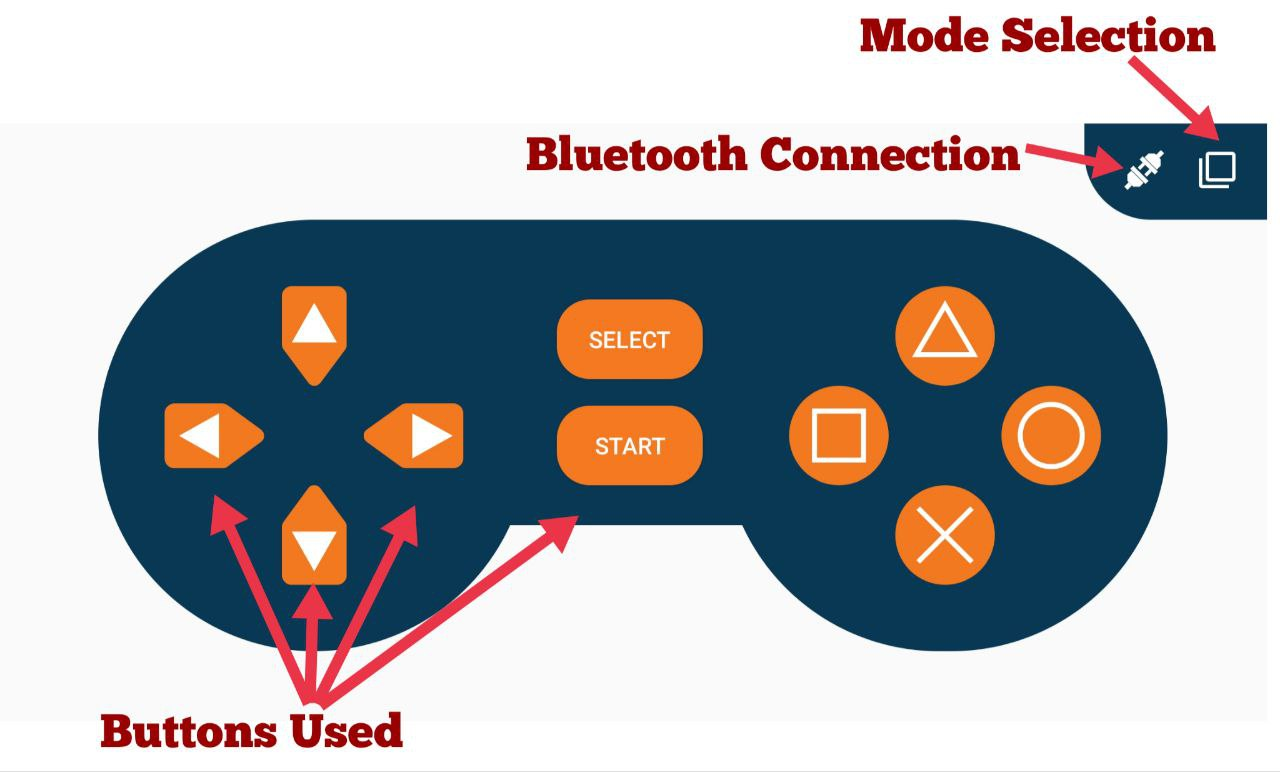
\includegraphics[width=\columnwidth]{vaman-esp32/bluetooth/figs/ble_app.jpg}
\caption{Dabble app Interface}
\label{fig:ble_app}
\end{figure}
\item Now connect the Seven Segment to the Vaman board according to the given
\autoref{table:ble-connections}
\begin{table}[!ht]
\centering
%%%%%%%%%%%%%%%%%%%%%%%%%%%%%%%%%%%%%%%%%%%%%%%%%%%%%%%%%%%%%%%%%%%%%%
%%                                                                  %%
%%  This is the header of a LaTeX2e file exported from Gnumeric.    %%
%%                                                                  %%
%%  This file can be compiled as it stands or included in another   %%
%%  LaTeX document. The table is based on the longtable package so  %%
%%  the longtable options (headers, footers...) can be set in the   %%
%%  preamble section below (see PRAMBLE).                           %%
%%                                                                  %%
%%  To include the file in another, the following two lines must be %%
%%  in the including file:                                          %%
%%        \def\inputGnumericTable{}                                 %%
%%  at the beginning of the file and:                               %%
%%        \input{name-of-this-file.tex}                             %%
%%  where the table is to be placed. Note also that the including   %%
%%  file must use the following packages for the table to be        %%
%%  rendered correctly:                                             %%
%%    \usepackage[latin1]{inputenc}                                 %%
%%    \usepackage{color}                                            %%
%%    \usepackage{array}                                            %%
%%    \usepackage{longtable}                                        %%
%%    \usepackage{calc}                                             %%
%%    \usepackage{multirow}                                         %%
%%    \usepackage{hhline}                                           %%
%%    \usepackage{ifthen}                                           %%
%%  optionally (for landscape tables embedded in another document): %%
%%    \usepackage{lscape}                                           %%
%%                                                                  %%
%%%%%%%%%%%%%%%%%%%%%%%%%%%%%%%%%%%%%%%%%%%%%%%%%%%%%%%%%%%%%%%%%%%%%%



%%  This section checks if we are begin input into another file or  %%
%%  the file will be compiled alone. First use a macro taken from   %%
%%  the TeXbook ex 7.7 (suggestion of Han-Wen Nienhuys).            %%
\def\ifundefined#1{\expandafter\ifx\csname#1\endcsname\relax}


%%  Check for the \def token for inputed files. If it is not        %%
%%  defined, the file will be processed as a standalone and the     %%
%%  preamble will be used.                                          %%
\ifundefined{inputGnumericTable}

%%  We must be able to close or not the document at the end.        %%
	\def\gnumericTableEnd{\end{document}}


%%%%%%%%%%%%%%%%%%%%%%%%%%%%%%%%%%%%%%%%%%%%%%%%%%%%%%%%%%%%%%%%%%%%%%
%%                                                                  %%
%%  This is the PREAMBLE. Change these values to get the right      %%
%%  paper size and other niceties.                                  %%
%%                                                                  %%
%%%%%%%%%%%%%%%%%%%%%%%%%%%%%%%%%%%%%%%%%%%%%%%%%%%%%%%%%%%%%%%%%%%%%%

	\documentclass[12pt%
			  %,landscape%
                    ]{report}
       \usepackage[latin1]{inputenc}
       \usepackage{fullpage}
       \usepackage{color}
       \usepackage{array}
       \usepackage{longtable}
       \usepackage{calc}
       \usepackage{multirow}
       \usepackage{hhline}
       \usepackage{ifthen}

	\begin{document}


%%  End of the preamble for the standalone. The next section is for %%
%%  documents which are included into other LaTeX2e files.          %%
\else

%%  We are not a stand alone document. For a regular table, we will %%
%%  have no preamble and only define the closing to mean nothing.   %%
    \def\gnumericTableEnd{}

%%  If we want landscape mode in an embedded document, comment out  %%
%%  the line above and uncomment the two below. The table will      %%
%%  begin on a new page and run in landscape mode.                  %%
%       \def\gnumericTableEnd{\end{landscape}}
%       \begin{landscape}


%%  End of the else clause for this file being \input.              %%
\fi

%%%%%%%%%%%%%%%%%%%%%%%%%%%%%%%%%%%%%%%%%%%%%%%%%%%%%%%%%%%%%%%%%%%%%%
%%                                                                  %%
%%  The rest is the gnumeric table, except for the closing          %%
%%  statement. Changes below will alter the table's appearance.     %%
%%                                                                  %%
%%%%%%%%%%%%%%%%%%%%%%%%%%%%%%%%%%%%%%%%%%%%%%%%%%%%%%%%%%%%%%%%%%%%%%

\providecommand{\gnumericmathit}[1]{#1} 
%%  Uncomment the next line if you would like your numbers to be in %%
%%  italics if they are italizised in the gnumeric table.           %%
%\renewcommand{\gnumericmathit}[1]{\mathit{#1}}
\providecommand{\gnumericPB}[1]%
{\let\gnumericTemp=\\#1\let\\=\gnumericTemp\hspace{0pt}}
 \ifundefined{gnumericTableWidthDefined}
        \newlength{\gnumericTableWidth}
        \newlength{\gnumericTableWidthComplete}
        \newlength{\gnumericMultiRowLength}
        \global\def\gnumericTableWidthDefined{}
 \fi
%% The following setting protects this code from babel shorthands.  %%
 \ifthenelse{\isundefined{\languageshorthands}}{}{\languageshorthands{english}}
%%  The default table format retains the relative column widths of  %%
%%  gnumeric. They can easily be changed to c, r or l. In that case %%
%%  you may want to comment out the next line and uncomment the one %%
%%  thereafter                                                      %%
\providecommand\gnumbox{\makebox[0pt]}
%%\providecommand\gnumbox[1][]{\makebox}

%% to adjust positions in multirow situations                       %%
\setlength{\bigstrutjot}{\jot}
\setlength{\extrarowheight}{\doublerulesep}

%%  The \setlongtables command keeps column widths the same across  %%
%%  pages. Simply comment out next line for varying column widths.  %%
\setlongtables

\setlength\gnumericTableWidth{%
	152pt+%
	140pt+%
0pt}
\def\gumericNumCols{2}
\setlength\gnumericTableWidthComplete{\gnumericTableWidth+%
         \tabcolsep*\gumericNumCols*2+\arrayrulewidth*\gumericNumCols}
\ifthenelse{\lengthtest{\gnumericTableWidthComplete > \linewidth}}%
         {\def\gnumericScale{1*\ratio{\linewidth-%
                        \tabcolsep*\gumericNumCols*2-%
                        \arrayrulewidth*\gumericNumCols}%
{\gnumericTableWidth}}}%
{\def\gnumericScale{1}}

%%%%%%%%%%%%%%%%%%%%%%%%%%%%%%%%%%%%%%%%%%%%%%%%%%%%%%%%%%%%%%%%%%%%%%
%%                                                                  %%
%% The following are the widths of the various columns. We are      %%
%% defining them here because then they are easier to change.       %%
%% Depending on the cell formats we may use them more than once.    %%
%%                                                                  %%
%%%%%%%%%%%%%%%%%%%%%%%%%%%%%%%%%%%%%%%%%%%%%%%%%%%%%%%%%%%%%%%%%%%%%%

\ifthenelse{\isundefined{\gnumericColA}}{\newlength{\gnumericColA}}{}\settowidth{\gnumericColA}{\begin{tabular}{@{}p{152pt*\gnumericScale}@{}}x\end{tabular}}
\ifthenelse{\isundefined{\gnumericColB}}{\newlength{\gnumericColB}}{}\settowidth{\gnumericColB}{\begin{tabular}{@{}p{140pt*\gnumericScale}@{}}x\end{tabular}}

\begin{longtable}[c]{%
	b{\gnumericColA}%
	b{\gnumericColB}%
	}

%%%%%%%%%%%%%%%%%%%%%%%%%%%%%%%%%%%%%%%%%%%%%%%%%%%%%%%%%%%%%%%%%%%%%%
%%  The longtable options. (Caption, headers... see Goosens, p.124) %%
%	\caption{The Table Caption.}             \\	%
% \hline	% Across the top of the table.
%%  The rest of these options are table rows which are placed on    %%
%%  the first, last or every page. Use \multicolumn if you want.    %%

%%  Header for the first page.                                      %%
%	\multicolumn{2}{c}{The First Header} \\ \hline 
%	\multicolumn{1}{c}{colTag}	%Column 1
%	&\multicolumn{1}{c}{colTag}	\\ \hline %Last column
%	\endfirsthead

%%  The running header definition.                                  %%
%	\hline
%	\multicolumn{2}{l}{\ldots\small\slshape continued} \\ \hline
%	\multicolumn{1}{c}{colTag}	%Column 1
%	&\multicolumn{1}{c}{colTag}	\\ \hline %Last column
%	\endhead

%%  The running footer definition.                                  %%
%	\hline
%	\multicolumn{2}{r}{\small\slshape continued\ldots} \\
%	\endfoot

%%  The ending footer definition.                                   %%
%	\multicolumn{2}{c}{That's all folks} \\ \hline 
%	\endlastfoot
%%%%%%%%%%%%%%%%%%%%%%%%%%%%%%%%%%%%%%%%%%%%%%%%%%%%%%%%%%%%%%%%%%%%%%

\hhline{|-|-}
	 \multicolumn{1}{|p{\gnumericColA}|}%
	{\gnumericPB{\centering}\textbf{VAMAN ESP pins}}
	&\multicolumn{1}{p{\gnumericColB}|}%
	{\gnumericPB{\centering}\textbf{Seven Segment pins}}
\\
\hhline{|--|}
	 \multicolumn{1}{|p{\gnumericColA}|}%
	{\gnumericPB{\centering}IO-32}
	&\multicolumn{1}{p{\gnumericColB}|}%
	{\gnumericPB{\centering}a}
\\
\hhline{|--|}
	 \multicolumn{1}{|p{\gnumericColA}|}%
	{\gnumericPB{\centering}IO-33}
	&\multicolumn{1}{p{\gnumericColB}|}%
	{\gnumericPB{\centering}b}
\\
\hhline{|--|}
	 \multicolumn{1}{|p{\gnumericColA}|}%
	{\gnumericPB{\centering}\gnumbox{IO-25}}
	&\multicolumn{1}{p{\gnumericColB}|}%
	{\gnumericPB{\centering}\gnumbox{c}}
\\
\hhline{|--|}
	 \multicolumn{1}{|p{\gnumericColA}|}%
	{\gnumericPB{\centering}\gnumbox{IO-26}}
	&\multicolumn{1}{p{\gnumericColB}|}%
	{\gnumericPB{\centering}\gnumbox{d}}
\\
\hhline{|--|}
	 \multicolumn{1}{|p{\gnumericColA}|}%
	{\gnumericPB{\centering}\gnumbox{IO-27}}
	&\multicolumn{1}{p{\gnumericColB}|}%
	{\gnumericPB{\centering}\gnumbox{e}}
\\
\hhline{|--|}
	 \multicolumn{1}{|p{\gnumericColA}|}%
	{\gnumericPB{\centering}\gnumbox{IO-14}}
	&\multicolumn{1}{p{\gnumericColB}|}%
	{\gnumericPB{\centering}\gnumbox{f}}
\\
\hhline{|--|}
	 \multicolumn{1}{|p{\gnumericColA}|}%
	{\gnumericPB{\centering}\gnumbox{IO-12}}
	&\multicolumn{1}{p{\gnumericColB}|}%
	{\gnumericPB{\centering}\gnumbox{g}}
\\
\hhline{|-|-|}
\end{longtable}

\ifthenelse{\isundefined{\languageshorthands}}{}{\languageshorthands{\languagename}}
\gnumericTableEnd

\caption{Connections}
\label{table:ble-connections}
\end{table}
\item Now you can observe the changes on seven segment display for Start, Up,
Down, Right and Left keys pressed on the Digital Mode on the android application
\end{enumerate}

\section{WiFi-Controlled Seven Segment Display}
This section demonstrates how to control the Seven Segment Display through the
Dabble Android application using WiFi and display on the seven segment according
to the controls in the Android app.

\subsection{Connections}
\begin{enumerate}
\item \textbf{Note}: \autoref{table:ble-components} and
\autoref{fig:vaman/uart/1}, \autoref{table:ble-connections} are similar to the
bluetooth control seven segment display.
\item Now, execute the following code
\item Make sure that change your "ssid","password" in code 
\begin{lstlisting}
vaman-esp32/wifi/codes/src
\end{lstlisting}
\item Build ESP32 firmware.
\begin{lstlisting}
cd vaman-esp32/wifi/codes
pio run 
\end{lstlisting}
\item Flash ESP32 firmware (connect Arduino-UART).
\begin{lstlisting}
pio run -t upload
\end{lstlisting}
\item Now check that your mobile/tab is connected with ESP32.
\item Install the WiFi Dabble app.
\begin{lstlisting}
vaman-esp32/wifi/Wifi_dabble.apk
\end{lstlisting}

\item Open the Dabble application. Enter the Vaman-ESP32 IP address as shown 
in \autoref{fig:dabble}.
\begin{figure}[!ht]
\centering
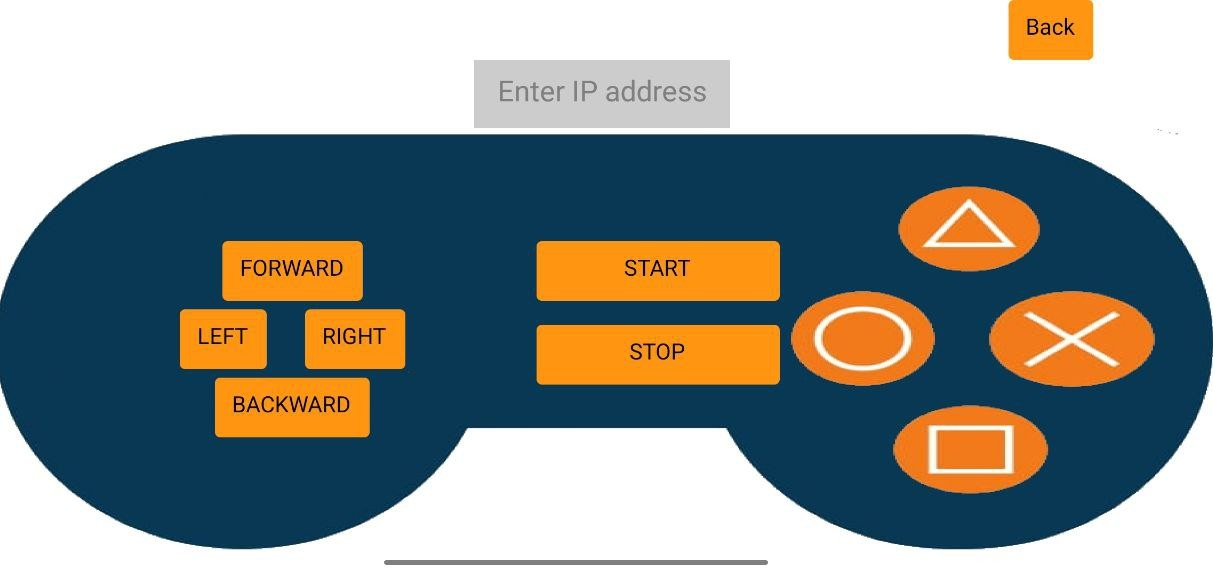
\includegraphics[width=0.6\columnwidth]{vaman-esp32/wifi/figs/wifi.jpg}
\caption{Wifi Dabble app}
\label{fig:dabble}
\end{figure}
\item Now you can observe the changes on seven-segment display for Start, Up, 
Down, Right and Left keys pressed on the Android application.
\end{enumerate}
\chapter{Maths computing using ESP32}
This chapter will demonstrate how to solve math problems using esp.
\section{Math Computing using ESP32}

\begin{enumerate}[label=\thesection.\arabic*.,ref=\thesection.\theenumi]

	\item Show that the points A $\myvec{1\\-2\\-8}$, B $\myvec{5\\0\\-2}$ and C $\myvec{11\\3\\7}$ are collinear, and find the ratio in which B divides AC.\\


\solution \\The input parameters for this problem are available in Table \ref{Table-1}
\begin{table}[ht!]
%%%%%%%%%%%%%%%%%%%%%%%%%%%%%%%%%%%%%%%%%%%%%%%%%%%%%%%%%%%%%%%%%%%%%%
%%                                                                  %%
%%  This is the header of a LaTeX2e file exported from Gnumeric.    %%
%%                                                                  %%
%%  This file can be compiled as it stands or included in another   %%
%%  LaTeX document. The table is based on the longtable package so  %%
%%  the longtable options (headers, footers...) can be set in the   %%
%%  preamble section below (see PRAMBLE).                           %%
%%                                                                  %%
%%  To include the file in another, the following two lines must be %%
%%  in the including file:                                          %%
%%        \def\inputGnumericTable{}                                 %%
%%  at the beginning of the file and:                               %%
%%        \input{name-of-this-file.tex}                             %%
%%  where the table is to be placed. Note also that the including   %%
%%  file must use the following packages for the table to be        %%
%%  rendered correctly:                                             %%
%%    \usepackage[latin1]{inputenc}                                 %%
%%    \usepackage{color}                                            %%
%%    \usepackage{array}                                            %%
%%    \usepackage{longtable}                                        %%
%%    \usepackage{calc}                                             %%
%%    \usepackage{multirow}                                         %%
%%    \usepackage{hhline}                                           %%
%%    \usepackage{ifthen}                                           %%
%%  optionally (for landscape tables embedded in another document): %%
%%    \usepackage{lscape}                                           %%
%%                                                                  %%
%%%%%%%%%%%%%%%%%%%%%%%%%%%%%%%%%%%%%%%%%%%%%%%%%%%%%%%%%%%%%%%%%%%%%%

                                                                                                                                                                                                                                                                                                                                                                                                                                                                                                                                                                                                                                                                                                                                                                                                                                                                                                     

%%  This section checks if we are begin input into another file or  %%
%%  the file will be compiled alone. First use a macro taken from   %%
%%  the TeXbook ex 7.7 (suggestion of Han-Wen Nienhuys).            %%
\def\ifundefined#1{\expandafter\ifx\csname#1\endcsname\relax}


%%  Check for the \def token for inputed files. If it is not        %%
%%  defined, the file will be processed as a standalone and the     %%
%%  preamble will be used.                                          %%
\ifundefined{inputGnumericTable}

%%  We must be able to close or not the document at the end.        %%
	\def\gnumericTableEnd{\end{document}}


%%%%%%%%%%%%%%%%%%%%%%%%%%%%%%%%%%%%%%%%%%%%%%%%%%%%%%%%%%%%%%%%%%%%%%
%%                                                                  %%
%%  This is the PREAMBLE. Change these values to get the right      %%
%%  paper size and other niceties.                                  %%
%%                                                                  %%
%%%%%%%%%%%%%%%%%%%%%%%%%%%%%%%%%%%%%%%%%%%%%%%%%%%%%%%%%%%%%%%%%%%%%%

	\documentclass[12pt%
			  %,landscape%
                    ]{report}
       \usepackage[latin1]{inputenc}
       \usepackage{fullpage}
       \usepackage{color}
       \usepackage{array}
       \usepackage{longtable}
       \usepackage{calc}
       \usepackage{multirow}
       \usepackage{hhline}
       \usepackage{ifthen}

	\begin{document}


%%  End of the preamble for the standalone. The next section is for %%
%%  documents which are included into other LaTeX2e files.          %%
\else

%%  We are not a stand alone document. For a regular table, we will %%
%%  have no preamble and only define the closing to mean nothing.   %%
    \def\gnumericTableEnd{}

%%  If we want landscape mode in an embedded document, comment out  %%
%%  the line above and uncomment the two below. The table will      %%
%%  begin on a new page and run in landscape mode.                  %%
%       \def\gnumericTableEnd{\end{landscape}}
%       \begin{landscape}


%%  End of the else clause for this file being \input.              %%
\fi

%%%%%%%%%%%%%%%%%%%%%%%%%%%%%%%%%%%%%%%%%%%%%%%%%%%%%%%%%%%%%%%%%%%%%%
%%                                                                  %%
%%  The rest is the gnumeric table, except for the closing          %%
%%  statement. Changes below will alter the table's appearance.     %%
%%                                                                  %%
%%%%%%%%%%%%%%%%%%%%%%%%%%%%%%%%%%%%%%%%%%%%%%%%%%%%%%%%%%%%%%%%%%%%%%

\providecommand{\gnumericmathit}[1]{#1} 
%%  Uncomment the next line if you would like your numbers to be in %%
%%  italics if they are italizised in the gnumeric table.           %%
%\renewcommand{\gnumericmathit}[1]{\mathit{#1}}
\providecommand{\gnumericPB}[1]%
{\let\gnumericTemp=\\#1\let\\=\gnumericTemp\hspace{0pt}}
 \ifundefined{gnumericTableWidthDefined}
        \newlength{\gnumericTableWidth}
        \newlength{\gnumericTableWidthComplete}
        \newlength{\gnumericMultiRowLength}
        \global\def\gnumericTableWidthDefined{}
 \fi
%% The following setting protects this code from babel shorthands.  %%
 \ifthenelse{\isundefined{\languageshorthands}}{}{\languageshorthands{english}}
%%  The default table format retains the relative column widths of  %%
%%  gnumeric. They can easily be changed to c, r or l. In that case %%
%%  you may want to comment out the next line and uncomment the one %%
%%  thereafter                                                      %%
\providecommand\gnumbox{\makebox[0pt]}
%%\providecommand\gnumbox[1][]{\makebox}

%% to adjust positions in multirow situations                       %%
\setlength{\bigstrutjot}{\jot}
\setlength{\extrarowheight}{\doublerulesep}

%%  The \setlongtables command keeps column widths the same across  %%
%%  pages. Simply comment out next line for varying column widths.  %%
\setlongtables

\setlength\gnumericTableWidth{%
	53pt+%
	53pt+%
	82pt+%
	53pt+%
0pt}
\def\gumericNumCols{4}
\setlength\gnumericTableWidthComplete{\gnumericTableWidth+%
         \tabcolsep*\gumericNumCols*2+\arrayrulewidth*\gumericNumCols}
\ifthenelse{\lengthtest{\gnumericTableWidthComplete > \linewidth}}%
         {\def\gnumericScale{1*\ratio{\linewidth-%
                        \tabcolsep*\gumericNumCols*2-%
                        \arrayrulewidth*\gumericNumCols}%
{\gnumericTableWidth}}}%
{\def\gnumericScale{1}}

%%%%%%%%%%%%%%%%%%%%%%%%%%%%%%%%%%%%%%%%%%%%%%%%%%%%%%%%%%%%%%%%%%%%%%
%%                                                                  %%
%% The following are the widths of the various columns. We are      %%
%% defining them here because then they are easier to change.       %%
%% Depending on the cell formats we may use them more than once.    %%
%%                                                                  %%
%%%%%%%%%%%%%%%%%%%%%%%%%%%%%%%%%%%%%%%%%%%%%%%%%%%%%%%%%%%%%%%%%%%%%%

\ifthenelse{\isundefined{\gnumericColA}}{\newlength{\gnumericColA}}{}\settowidth{\gnumericColA}{\begin{tabular}{@{}p{53pt*\gnumericScale}@{}}x\end{tabular}}
\ifthenelse{\isundefined{\gnumericColB}}{\newlength{\gnumericColB}}{}\settowidth{\gnumericColB}{\begin{tabular}{@{}p{53pt*\gnumericScale}@{}}x\end{tabular}}
\ifthenelse{\isundefined{\gnumericColC}}{\newlength{\gnumericColC}}{}\settowidth{\gnumericColC}{\begin{tabular}{@{}p{82pt*\gnumericScale}@{}}x\end{tabular}}
\ifthenelse{\isundefined{\gnumericColD}}{\newlength{\gnumericColD}}{}\settowidth{\gnumericColD}{\begin{tabular}{@{}p{53pt*\gnumericScale}@{}}x\end{tabular}}

	\begin{center}
\begin{tabular}[c]{%
	b{\gnumericColA}%
	b{\gnumericColB}%
	b{\gnumericColC}%
	b{\gnumericColD}%
	}

%%%%%%%%%%%%%%%%%%%%%%%%%%%%%%%%%%%%%%%%%%%%%%%%%%%%%%%%%%%%%%%%%%%%%%
%%  The longtable options. (Caption, headers... see Goosens, p.124) %%
%	\caption{The Table Caption.}             \\	%
% \hline	% Across the top of the table.
%%  The rest of these options are table rows which are placed on    %%
%%  the first, last or every page. Use \multicolumn if you want.    %%

%%  Header for the first page.                                      %%
%	\multicolumn{4}{c}{The First Header} \\ \hline 
%	\multicolumn{1}{c}{colTag}	%Column 1
%	&\multicolumn{1}{c}{colTag}	%Column 2
%	&\multicolumn{1}{c}{colTag}	%Column 3
%	&\multicolumn{1}{c}{colTag}	\\ \hline %Last column
%	\endfirsthead

%%  The running header definition.                                  %%
%	\hline
%	\multicolumn{4}{l}{\ldots\small\slshape continued} \\ \hline
%	\multicolumn{1}{c}{colTag}	%Column 1
%	&\multicolumn{1}{c}{colTag}	%Column 2
%	&\multicolumn{1}{c}{colTag}	%Column 3
%	&\multicolumn{1}{c}{colTag}	\\ \hline %Last column
%	\endhead

%%  The running footer definition.                                  %%
%	\hline
%	\multicolumn{4}{r}{\small\slshape continued\ldots} \\
%	\endfoot

%%  The ending footer definition.                                   %%
%	\multicolumn{4}{c}{That's all folks} \\ \hline 
%	\endlastfoot
%%%%%%%%%%%%%%%%%%%%%%%%%%%%%%%%%%%%%%%%%%%%%%%%%%%%%%%%%%%%%%%%%%%%%%

\hhline{|-|-|-~}
	 \multicolumn{1}{|p{\gnumericColA}|}%
	{\gnumericPB{\centering}\gnumbox{\textbf{Symbol}}}
	&\multicolumn{1}{p{\gnumericColB}|}%
	{\gnumericPB{\centering}\gnumbox{\textbf{Value}}}
	&\multicolumn{1}{p{\gnumericColC}|}%
	{\gnumericPB{\centering}\gnumbox{\textbf{Description}}}
	&
\\
\hhline{|---|~}
	 \multicolumn{1}{|p{\gnumericColA}|}%
	{\gnumericPB{\centering}\gnumbox{$\vec{A}$}}
	&\multicolumn{1}{p{\gnumericColB}|}%
	{\gnumericPB{\centering}\gnumbox{$\myvec{1\\-2\\-8}$}}
	&\multicolumn{1}{p{\gnumericColC}|}%
	{\gnumericPB{\centering}\gnumbox{First point}}
	&
\\
\hhline{|---|~}
	 \multicolumn{1}{|p{\gnumericColA}|}%
	{\gnumericPB{\centering}\gnumbox{$\vec{B}$}}
	&\multicolumn{1}{p{\gnumericColB}|}%
	{\gnumericPB{\centering}\gnumbox{$\myvec{5\\0\\-2}$}}
	&\multicolumn{1}{p{\gnumericColC}|}%
	{\gnumericPB{\centering}\gnumbox{Second point}}
	&
\\
\hhline{|---|~}
	 \multicolumn{1}{|p{\gnumericColA}|}%
	{\gnumericPB{\centering}\gnumbox{$\vec{C}$}}
	&\multicolumn{1}{p{\gnumericColB}|}%
	{\gnumericPB{\centering}\gnumbox{$\myvec{11\\3\\7}$}}
	&\multicolumn{1}{p{\gnumericColC}|}%
	{\gnumericPB{\centering}\gnumbox{Third point}}
	&
\\
\hhline{|-|-|-|~}
\end{tabular}
	\end{center}

\ifthenelse{\isundefined{\languageshorthands}}{}{\languageshorthands{\languagename}}
\gnumericTableEnd

\caption{}
\label{Table-1}	

\end{table}

		Points $\vec{A}$, $\vec{B}$ and $\vec{C}$ are on a line if
    \begin{align}
        \textrm{rank}\myvec{\vec{A} & \vec{B} & \vec{C}} < 3
        \label{eq:chapters/12/10/5/8rank-collinear}
    \end{align}
    Substituting, we must find the rank of
    \begin{align}
        \vec{M} = \myvec{1&5&11\\-2&0&3\\-8&-2&7}
    \end{align}
    Using row reduction methods to bring $\vec{M}$ into row-reduced echelon form,
    \begin{align}
        \myvec{1&5&11\\-2&0&3\\-8&-2&7}&\xleftrightarrow[]{R_2\rightarrow R_2+2R_1}
        \myvec{1&5&11\\0&10&25\\-8&-2&7} \\
                &\xleftrightarrow[]{R_3\rightarrow R_3+8R_1}\myvec{1&5&11\\0&10&25\\0&38&95} \\
                &\xleftrightarrow[]{R_3\rightarrow R_3-\frac{19}{5}R_2}\myvec{1&5&11\\0&10&25\\0&0&0}
                \label{eq:chapters/12/10/5/8row-red}
    \end{align}
    Clearly, the rank of $\vec{M}$ is 2, and hence the given points are 
    collinear. 
    Fig. \ref{fig:Fig1}  verifies that the three points are indeed 
    collinear as claimed.\\
	Let $\vec{B}$ divide $\vec{AC}$ in k:1 then,
	\begin{align}
		\frac{k\vec{C}+\vec{A}}{k+1} = \vec{B}
	\end{align}
		\begin{align}
			\implies k\vec{C}+\vec{A}=\vec{B}\brak{k+1}
			\implies k\brak{\vec{C}-\vec{B}}=\brak{\vec{B}-\vec{A}}
		\end{align}
			Multiplying with $\brak{\vec{C}-\vec{B}}^{\top}$ on both sides,\\
	
		\begin{align*}
			 k\brak{\vec{C}-\vec{B}}\brak{\vec{C}-\vec{B}}^{\top}=\brak{\vec{B}-\vec{A}}{\vec{C}-\vec{B}}^{\top}
		\end{align*}
			The value of k is as follows,
			\begin{align}
			k &=
			\frac{\brak{\vec{B}-\vec{A}}\brak{\vec{C}-\vec{B}}^{\top}}{\norm{\vec{C-B}}^2}
			\end{align}
			where,
			\begin{align}
				\brak{\vec{B-A}} &=
				\brak{\myvec{5\\0\\-2}-\myvec{1\\-2\\-8}} =
				\myvec{4\\2\\6}
			\end{align}
			
			\begin{align}
				\brak{\vec{C-B}} &=
				\brak{\myvec{11\\3\\7}-\myvec{5\\0\\-2}} =
				\myvec{6\\3\\9}
			\end{align}
			\begin{align*}
				\brak{\vec{C}-\vec{B}}^{\top} &=
				\myvec{6 & 3 & 9}
			\end{align*}
			Substituting the values the value of $k$ is $2/3$.
			\\    Hence, $\vec{B}$ divides $\vec{AC}$ in the ratio $2:3$.
	\begin{figure}[!h]
		\begin{center}
			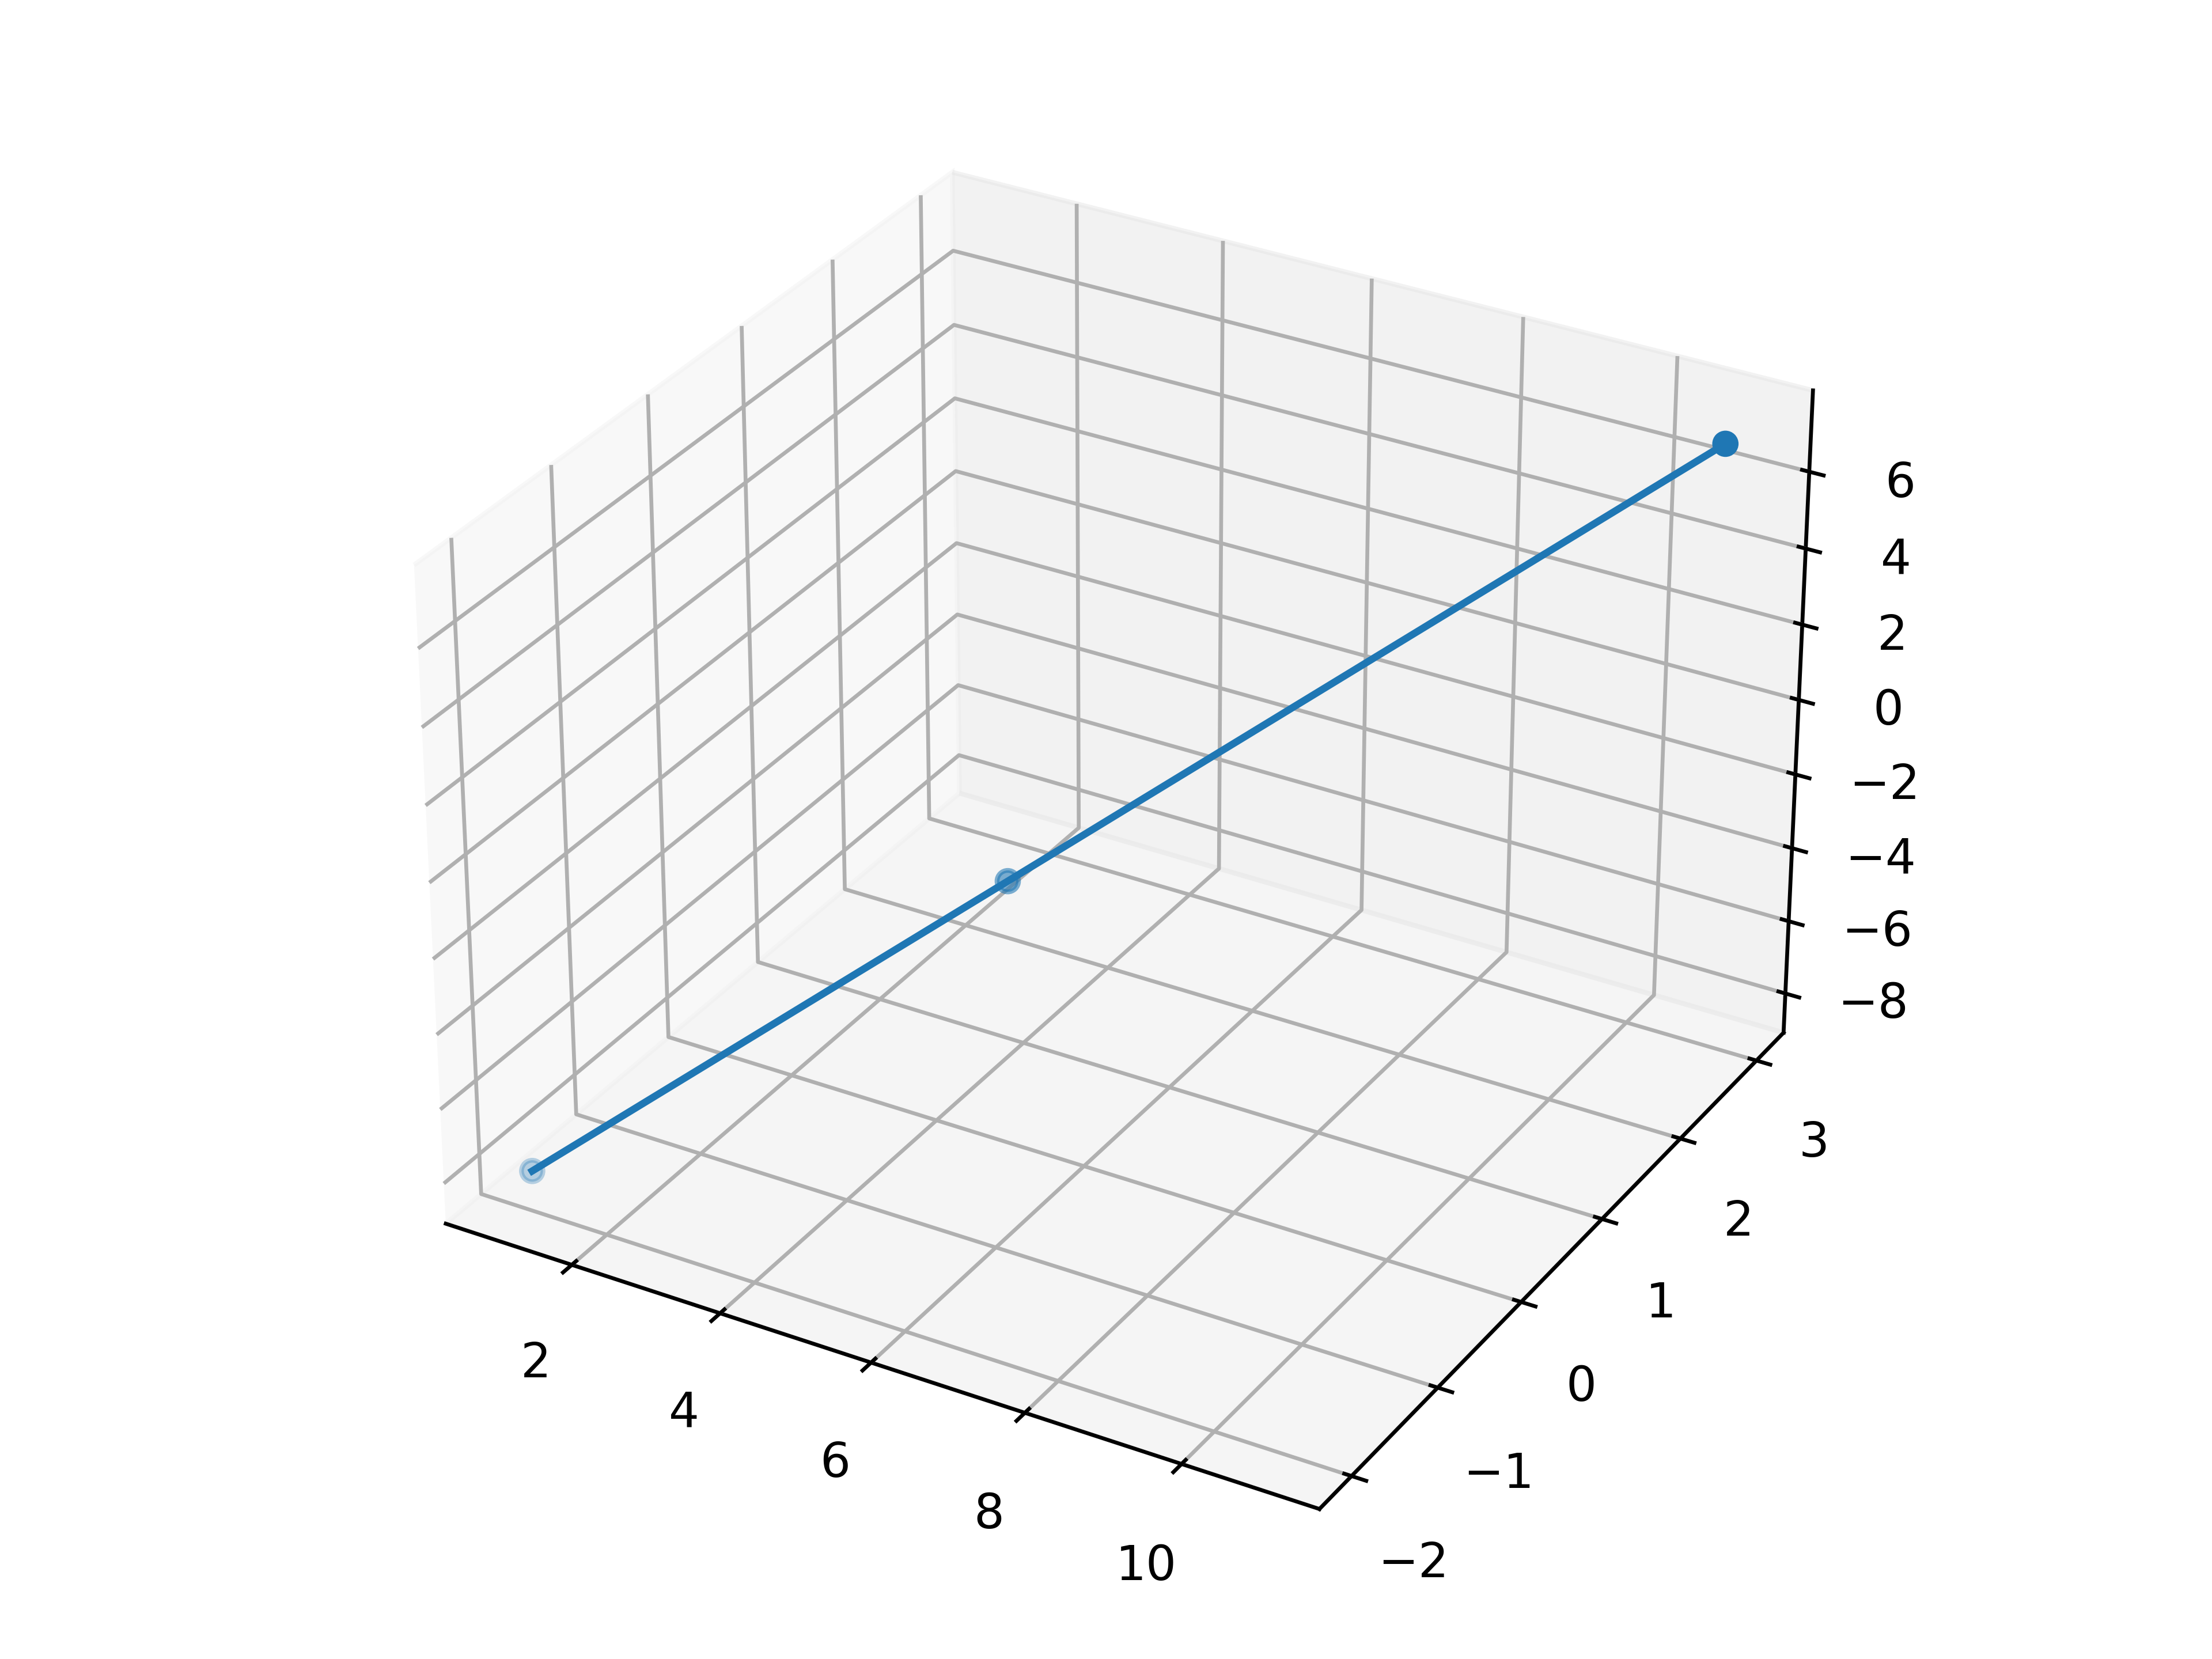
\includegraphics[width=\columnwidth]{./math_using_esp/figs/line_3d.png}
		\end{center}
		\caption{}
		\label{fig:Fig1}
	\end{figure}
\end{enumerate}

\begin{enumerate}[label=\thesection.\arabic*.,ref=\thesection.\theenumi]	
\subsection{C pointer code}
\item The following is the C code for the above question using pointers
\begin{lstlisting}
vaman/vaman-esp/math_using_esp/codes/cprog/main.c
\end{lstlisting}
\end{enumerate}

\begin{enumerate}[label=\thesection.\arabic*.,ref=\thesection.\theenumi]
\section{Code execution for Math Computing using esp32}
\raggedright
\item Now, Execute the following code
\begin{lstlisting}
math_using_esp/codes/esp_code/src/main.cpp
\end{lstlisting}
\item Build the ESP32 firmware
\begin{lstlisting}
cd  math_using_esp/codes/esp_code
pio run
\end{lstlisting} 
\item Flash ESP32 firmware ( using Arduino  )
\begin{lstlisting}
pio run -t upload
\end{lstlisting} 
\end{enumerate}

\subsection{Displaying the output  on website}
\begin{enumerate}[label=\thesection.\arabic*.,ref=\thesection.\theenumi]
\item The output of the code i.e; if the points are collinear or not will be displayed in the webserver.
\item After flashing the code to vaman-ESP, the board will be connected to the wifi credentials provided.
\item Now connect the same WiFi credentials to the mobile phone for accessing the IP address, which can be accessed by 
\begin{lstlisting}
ifconfig
nmap -sn 192.168.x.x/24
\end{lstlisting}
\item Change the IP address in the second command accordingly with the IP address provided by first command.
\item By the above commands the IP address of vaman-ESP will be diplayed.
\item Now the vaman-ESP will be hosting a webserver
\item In order to access the webserver type the IP address of the vaman-ESP in the web browser.
\item In the website loaded by the IP address of vaman-ESP the output is displayed as shown in Fig. \ref{fig:results of collinear}
\begin{figure}[H]
\centering
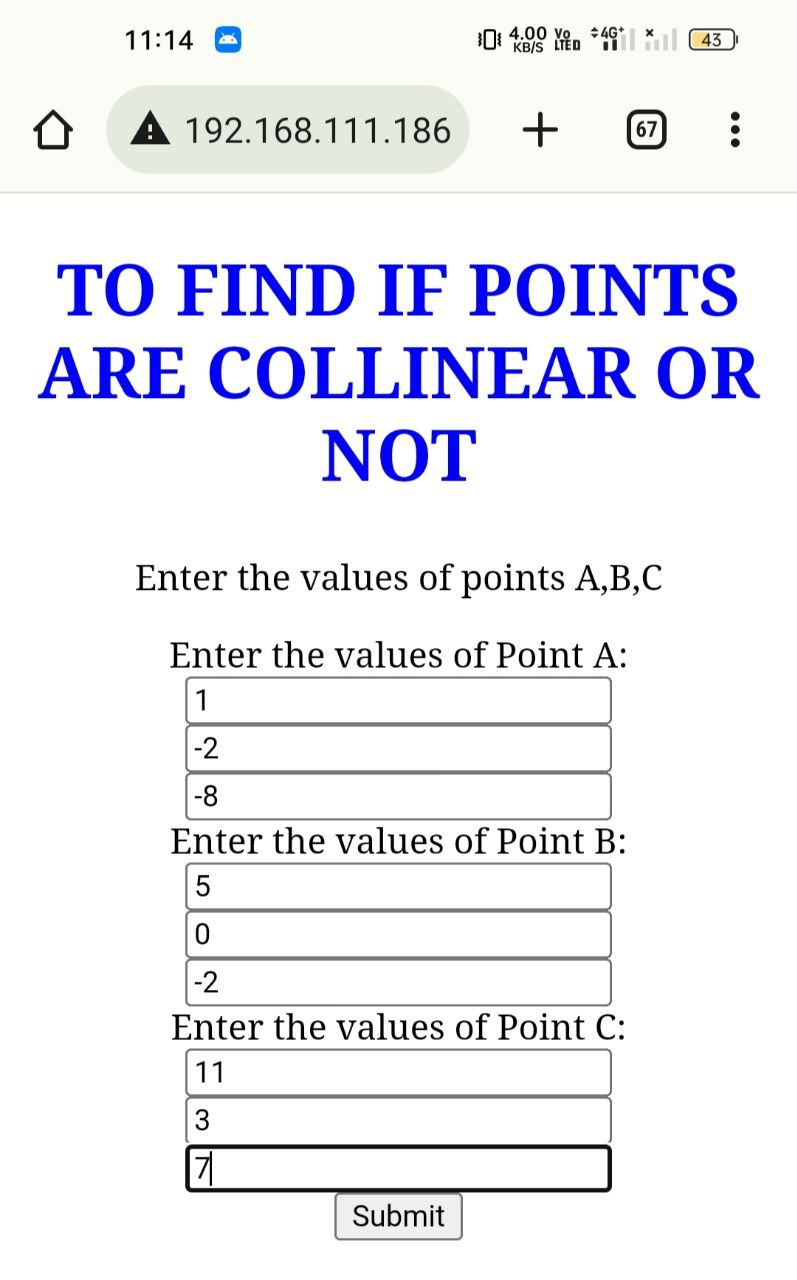
\includegraphics[scale =0.3]{./math_using_esp/figs/1.jpg}
\caption{Website}
\label{fig:results of collinear}
\end{figure}

\begin{figure}[H]
\centering
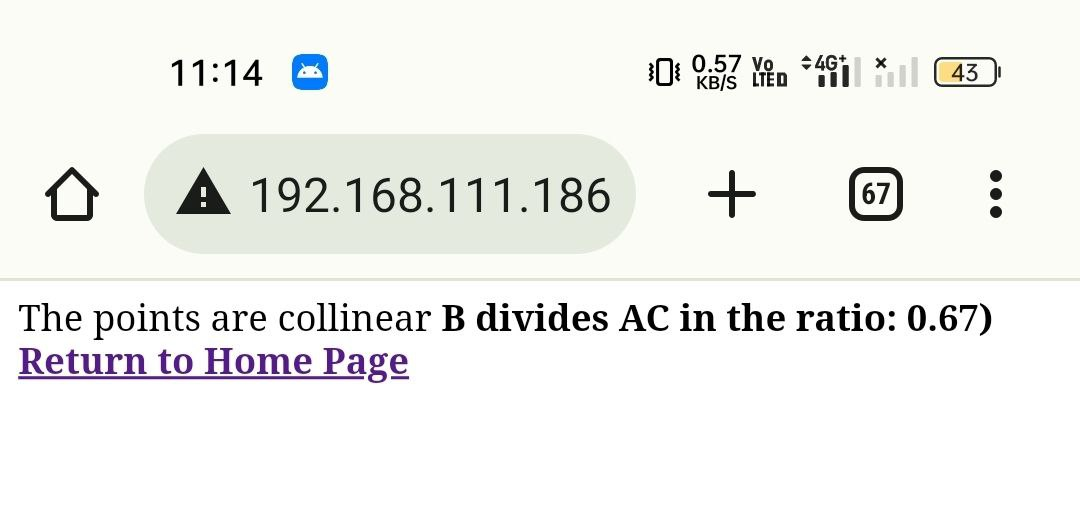
\includegraphics[width=\columnwidth]{./math_using_esp/figs/2.jpg}
\caption{Website result}
\label{fig:results of collinear equations }
\end{figure}

\end{enumerate}



\chapter{Inter-Chip Communication}
This chapter demonstrates how various platforms on the LC Vaman (ESP32, ARM,
FPGA) can communicate with each other through various protocols such as Serial
Peripheral Interface (SPI) and the AHB-To-Wishbone bridge on the Pygmy.
\section{ESP32 and FPGA}
This section describes various experiments that interface the ESP32 and eFPGA
present on the LC Vaman.
\subsection{Onboard LED}
This subsection illustrates the use of SPI Communication between the Vaman-ESP32
and the FPGA onboard the Vaman-Pygmy by toggling the LEDs onboard the
Vaman-Pygmy.

\subsubsection{Components}
\begin{table}[!ht]
    \centering
    \input{inter-chip/esp32-fpga/led/tables/components.tex}
    \caption{Components Required for Controlling the Onboard LED via SPI.}
    \label{tab:esp32-fpga-led-components}
\end{table}

\subsubsection{Connections}
\begin{table}[!ht]
    \centering
    \input{inter-chip/esp32-fpga/led/tables/connections.tex}
    \caption{Connections to establish SPI between Vaman-ESP32 and Vaman-Pygmy.}
    \label{tab:esp32-fpga-led-connections}
\end{table}

\subsubsection{Building}
\begin{enumerate}
    \item Build the PlatformIO project at
    \begin{lstlisting}
inter-chip/esp32-fpga/led/codes/esp32
    \end{lstlisting}
    \item Flash the project .bin file using USB-UART connected to the 
    Vaman-ESP32, via PlatformIO or ArduinoDroid.
    \item Build the FPGA project .bin file by entering the following commands at
    a terminal window.
    \begin{lstlisting}
# The following variable can be sourced from .shellrc or .venv/bin/activate
export QORC_SDK_PATH=/path/to/pygmy-sdk
cd inter-chip/esp32-fpga/led/codes/fpga
make
    \end{lstlisting}
    \item On building successfully, the file
    \begin{lstlisting}
inter-chip/esp32-fpga/led/codes/fpga/rtl/AL4S3B_FPGA_Top.bin
    \end{lstlisting}
    is generated.
    \item Flash the .bin file to the Vaman-Pygmy by resetting it to bootloader
    mode and entering the following command at a terminal window.
    \begin{lstlisting}
python3 /path/to/tinyfpga-programmer-gui.py --port /dev/ttyACMxx --mode fpga --appfpga /path/to/AL4S3B_FPGA_Top.bin --reset
    \end{lstlisting}
    where /dev/ttyACMxx is the port at which the Vaman board is available. This
    can be obtained by inspecting the output of the following command (requires
    root/sudo privileges).
    \begin{lstlisting}
dmesg -w
    \end{lstlisting}
\end{enumerate}

\subsubsection{Demonstration}
\begin{enumerate}
    \item Find the IP address of the Vaman-ESP32 by inspecting the output of the
    serial terminal, or by typing at a terminal window
    \begin{lstlisting}
ifconfig
nmap -sn xx.yy.zz.0/24
    \end{lstlisting}
    where xx.yy.zz represents the first three octets of the IP address of your
    device on the WiFi network interface, found using \texttt{ifconfig}.
    \item Then, go to the site
    \begin{lstlisting}
http://<VAMAN-IP>/led
    \end{lstlisting}
    and interact with the radio buttons to toggle the LEDs onboard the
    Vaman-Pygmy. 
\end{enumerate}

\subsubsection{Exercises}
\begin{enumerate}
    \item Modify the ESP32 code to have three separate radio buttons for each
    onboard LED.
    \item Modify the ESP32 code to blink the LED periodically when the user
    toggles a checkbox on the HTML form.
    \item SPI transactions are a bottleneck in execution. Try to minimize the
    number of SPI transactions and the amount of data transmitted in each of
    them.
\end{enumerate}
\subsection{Seven-Segment Display}
This subsection illustrates the use of SPI Communication between the Vaman-ESP32
and the FPGA onboard the Vaman-Pygmy by controlling a seven segment display 
remotely.

\subsubsection{Components}
\begin{table}[!ht]
    \centering
    \input{inter-chip/esp32-fpga/sevenseg/tables/components.tex}
    \caption{Components Required for Controlling the Onboard LED via SPI.}
    \label{tab:esp32-fpga-sevenseg-components}
\end{table}

\subsubsection{Connections}
\begin{table}[!ht]
    \centering
    \input{inter-chip/esp32-fpga/sevenseg/tables/vaman-connections.tex}
    \caption{Connections to establish SPI between Vaman-ESP32 and Vaman-Pygmy.}
    \label{tab:esp32-fpga-sevenseg-vaman-connections}
\end{table}

\begin{table}[!ht]
    \centering
    \input{inter-chip/esp32-fpga/sevenseg/tables/sevenseg-connections.tex}
    \caption{Connections to interface seven-segment display with Vaman-Pygmy.}
    \label{tab:esp32-fpga-sevenseg-display-connections}
\end{table}

\subsubsection{Building}
\begin{enumerate}
    \item Build the PlatformIO project at
    \begin{lstlisting}
inter-chip/esp32-fpga/sevenseg/codes/esp32
    \end{lstlisting}
    \item Flash the project .bin file using USB-UART connected to the 
    Vaman-ESP32, via PlatformIO or ArduinoDroid.
    \item Build the FPGA project .bin file by entering the following commands at
    a terminal window.
    \begin{lstlisting}
# The following variable can be sourced from .shellrc or .venv/bin/activate
export QORC_SDK_PATH=/path/to/pygmy-sdk
cd inter-chip/esp32-fpga/sevenseged/codes/fpga
make
    \end{lstlisting}
    \item On building successfully, the file
    \begin{lstlisting}
inter-chip/esp32-fpga/sevenseg/codes/fpga/rtl/AL4S3B_FPGA_Top.bin
    \end{lstlisting}
    is generated.
    \item Flash the .bin file to the Vaman-Pygmy by resetting it to bootloader
    mode and entering the following command at a terminal window.
    \begin{lstlisting}
python3 /path/to/tinyfpga-programmer-gui.py --port /dev/ttyACMxx --mode fpga --appfpga /path/to/AL4S3B_FPGA_Top.bin --reset
    \end{lstlisting}
    where /dev/ttyACMxx is the port at which the Vaman board is available. This
    can be obtained by inspecting the output of the following command (requires
    root/sudo privileges).
    \begin{lstlisting}
dmesg -w
    \end{lstlisting}
\end{enumerate}

\subsubsection{Demonstration}
\begin{enumerate}
    \item Find the IP address of the Vaman-ESP32 by inspecting the output of the
    serial terminal, or by typing at a terminal window
    \begin{lstlisting}
ifconfig
nmap -sn xx.yy.zz.0/24
    \end{lstlisting}
    where xx.yy.zz represents the first three octets of the IP address of your
    device on the WiFi network interface, found using \texttt{ifconfig}.
    \item Then, go to the site
    \begin{lstlisting}
http://<VAMAN-IP>/sevenseg
    \end{lstlisting}
    and interact with the HTML form to see the output on the seven-segment
    display.
\end{enumerate}

\subsubsection{Exercises}
\begin{enumerate}
    \item Modify the ESP32 code to have seven separate radio buttons for each
    segment. Additionally, you can also have another button for the dot.
    \item Try to minimize the number of SPI transactions and the amount of data
    transmitted in each of them.
\end{enumerate}
\section{FPGA and M4}
This section describes various experiments that can be performed by interfacing
the M4 and eFPGA susystems on the Vaman-Pygmy.
\subsection{Onboard LED}
This subsection illustrates the interface between the ARM Cortex-M4 subsystem
and the eFPGA subsystem onboard the Vaman-Pygmy through a blink program, where
the GPIO pins corresponding to the onboard LEDs are exposed by the FPGA
platform.

\subsubsection{Components}
\begin{table}[!ht]
    \centering
    \input{inter-chip/m4-fpga/blink/tables/components.tex}
    \caption{Components Required for Controlling the Onboard LED.}
    \label{tab:esp32-m4-fpga-blink-components}
\end{table}

\subsubsection{Building}
\begin{enumerate}
    \item Build the FPGA project .bin file by entering the following commands at
    a terminal window.
    \begin{lstlisting}
# The following variable can be sourced from .shellrc or .venv/bin/activate
export QORC_SDK_PATH=/path/to/pygmy-sdk
cd inter-chip/m4-fpga/blink/codes/fpga
make
    \end{lstlisting}
    \item On building successfully, the file
    \begin{lstlisting}
inter-chip/m4-fpga/blink/codes/fpga/rtl/AL4S3B_FPGA_Top.bin
    \end{lstlisting}
    is generated.
    \item Edit the variable PROJ\_ROOT in
    \begin{lstlisting}
inter-chip/m4-fpga/blink/codes/m4/GCC_Project/config.mk
    \end{lstlisting}
    to point to the location of the pygmy-sdk folder on your system.
    \item Build the M4 project .bin file by entering the following commands at a
    terminal window.
    \begin{lstlisting}
cd inter-chip/m4-fpga/blink/codes/m4/GCC_Project
make -j4
    \end{lstlisting}
    \item On building successfully, the file
    \begin{lstlisting}
inter-chip/m4-fpga/blink/codes/m4/GCC_Project/output/bin/m4.bin
    \end{lstlisting}
    is generated.
    \item Flash both FPGA and M4 .bin files to the Vaman-Pygmy by resetting it
    to bootloader mode and entering the following command at a terminal window.
    \begin{lstlisting}
python3 /path/to/tinyfpga-programmer-gui.py --port /dev/ttyACMxx --mode m4-fpga --m4app /path/to/m4.bin --appfpga /path/to/AL4S3B_FPGA_Top.bin --reset
    \end{lstlisting}
    where /dev/ttyACMxx is the port at which the Vaman board is available. This
    can be obtained by inspecting the output of the following command (requires
    root/sudo privileges).
    \begin{lstlisting}
dmesg -w
    \end{lstlisting}
\end{enumerate}

\subsubsection{Demonstration}
All three LEDs onboard the Vaman will toggle every one second when the Vaman
boots normally.

\subsubsection{Exercises}
\begin{enumerate}
    \item Find out the addresses corresponding to the GPIO module by inspecting
    the code in pygmy-sdk, as well as in this folder.
    \item Create code to blink each LED in turn.
\end{enumerate}
\subsection{Seven-Segment Display}
This subsection demonstrates the interface between the M4 subsystem and eFPGA
subsystem on the Vaman-Pygmy by controlling a seven-segment display, where the
GPIO interface is exposed to the M4 by the FPGA platform.

\subsubsection{Components}
\begin{table}[!ht]
    \centering
    \input{inter-chip/m4-fpga/sevenseg/tables/components.tex}
    \caption{Components Required for Controlling the Onboard LED.}
    \label{tab:m4-fpga-sevenseg-components}
\end{table}

\subsubsection{Connections}
\begin{table}[!ht]
    \centering
    \input{inter-chip/m4-fpga/sevenseg/tables/sevenseg-connections.tex}
    \caption{Connections for interfacing the seven-segment display with Vaman-Pygmy.}
    \label{tab:m4-fpga-sevenseg-connections}
\end{table}

\subsubsection{Building}
\begin{enumerate}
    \item Build the FPGA project .bin file by entering the following commands at
    a terminal window.
    \begin{lstlisting}
# The following variable can be sourced from .shellrc or .venv/bin/activate
export QORC_SDK_PATH=/path/to/pygmy-sdk
cd inter-chip/m4-fpga/sevenseg/codes/fpga
make
    \end{lstlisting}
    \item On building successfully, the file
    \begin{lstlisting}
inter-chip/m4-fpga/sevenseg/codes/fpga/rtl/AL4S3B_FPGA_Top.bin
    \end{lstlisting}
    is generated.
    \item Edit the variable PROJ\_ROOT in
    \begin{lstlisting}
inter-chip/m4-fpga/sevenseg/codes/m4/GCC_Project/config.mk
    \end{lstlisting}
    to point to the location of the pygmy-sdk folder on your system.
    \item Build the M4 project .bin file by entering the following commands at a
    terminal window.
    \begin{lstlisting}
cd inter-chip/m4-fpga/sevenseg/codes/m4/GCC_Project
make -j4
    \end{lstlisting}
    \item On building successfully, the file
    \begin{lstlisting}
inter-chip/m4-fpga/sevenseg/codes/m4/GCC_Project/output/bin/m4.bin
    \end{lstlisting}
    is generated.
    \item Flash both FPGA and M4 .bin files to the Vaman-Pygmy by resetting it
    to bootloader mode and entering the following command at a terminal window.
    \begin{lstlisting}
python3 /path/to/tinyfpga-programmer-gui.py --port /dev/ttyACMxx --mode m4-fpga --m4app /path/to/m4.bin --appfpga /path/to/AL4S3B_FPGA_Top.bin --reset
    \end{lstlisting}
    where /dev/ttyACMxx is the port at which the Vaman board is available. This
    can be obtained by inspecting the output of the following command (requires
    root/sudo privileges).
    \begin{lstlisting}
dmesg -w
    \end{lstlisting}
\end{enumerate}

\subsubsection{Demonstration}
All three LEDs onboard the Vaman will toggle every one second when the Vaman
boots normally.

\subsubsection{Exercises}
\begin{enumerate}[resume]
    \item Create a decade counter with this interface.
    \item Extend the code to accommodate hexadecimal digits.
\end{enumerate}
\subsection{Binary-Coded Decimal Decoder}
This subsection demonstrates the interface between the M4 subsystem and eFPGA
subsystem on the Vaman-Pygmy by simulating a Binary-Coded Decimal (BCD) Decoder,
otherwise known as a 7447 IC. The GPIO interface is exposed to the M4 by the
FPGA platform.

\subsubsection{Components}
The components required are listed in \autoref{tab:m4-fpga-bcd-components}.
\begin{table}[!ht]
    \centering
    \input{inter-chip/m4-fpga/bcd/tables/components.tex}
    \caption{Components Required for Simulating the 7447 IC.}
    \label{tab:m4-fpga-bcd-components}
\end{table}

\subsubsection{Connections}
The connections to be made between the seven-segment display and Vaman board are
listed in \autoref{tab:esp32-fpga-sevenseg-display-connections}. The equivalent
7447 IC input pins are listed in \autoref{tab:m4-fpga-bcd-bcd-connections}.

\begin{table}[!ht]
    \centering
    \input{inter-chip/m4-fpga/bcd/tables/bcd-connections.tex}
    \caption{Equivalent Input Pins for the 7447 IC on the Vaman-Pygmy.}
    \label{tab:m4-fpga-bcd-bcd-connections}
\end{table}

\subsubsection{Building}
\begin{enumerate}
    \item Build the FPGA project .bin file by entering the following commands at
    a terminal window.
    \begin{lstlisting}
# The following variable can be sourced from .shellrc or .venv/bin/activate
export QORC_SDK_PATH=/path/to/pygmy-sdk
cd inter-chip/m4-fpga/bcd/codes/fpga
make
    \end{lstlisting}
    \item On building successfully, the .bin file is generated at
    \begin{lstlisting}
inter-chip/m4-fpga/bcd/codes/fpga/rtl/AL4S3B_FPGA_Top.bin
    \end{lstlisting}
    \item Edit the variable PROJ\_ROOT to point to the location of the pygmy-sdk
    folder on your system in the file
    \begin{lstlisting}
inter-chip/m4-fpga/bcd/codes/m4/GCC_Project/config.mk
    \end{lstlisting}
    \item Build the M4 project .bin file by entering the following commands at a
    terminal window.
    \begin{lstlisting}
cd inter-chip/m4-fpga/bcd/codes/m4/GCC_Project
make -j4
    \end{lstlisting}
    \item On building successfully, the .bin file is generated at
    \begin{lstlisting}
inter-chip/m4-fpga/bcd/codes/m4/GCC_Project/output/bin/m4.bin
    \end{lstlisting}
    \item Flash both FPGA and M4 .bin files to the Vaman-Pygmy by resetting it
    to bootloader mode and entering the following command at a terminal window
    \begin{lstlisting}
python3 /path/to/tinyfpga-programmer-gui.py --port /dev/ttyACMxx --mode m4-fpga --m4app /path/to/m4.bin --appfpga /path/to/AL4S3B_FPGA_Top.bin --reset
    \end{lstlisting}
    where /dev/ttyACMxx is the port at which the Vaman board is available. This
    can be obtained by inspecting the output of the following command (requires
    root/sudo privileges).
    \begin{lstlisting}
dmesg -w
    \end{lstlisting}
\end{enumerate}

\subsubsection{Demonstration}
Give an input to the BCD by connecting the male ends of the jumpers at pins 10
to 13 on the Vaman-Pygmy to high voltage or ground. The equivalent digit should
be displayed on the seven-segment display.

\subsubsection{Exercises}
\begin{enumerate}[resume]
    \item Create code for an incrementing encoder instead of a display decoder.
    \item Extend the code to perform mathematical operations modulo 10 and
    display the result.
    \item Extend the code to accommodate hexadecimal digits.
\end{enumerate}
\section{ESP32, FPGA and M4}
This section describes various experiments that can be performed by interfacing
all three platforms, ESP32, FPGA and M4 onboard the LC Vaman.
\subsection{Onboard LED}
This subsection illustrates the use of SPI Communication between the Vaman-ESP32
and the ARM Cortex-M4 subsystem onboard the Vaman-Pygmy by toggling the LEDs via
the ARM interface, where the GPIO pins are exposed by the FPGA platform.

\subsubsection{Components}
\begin{table}[!ht]
    \centering
    \input{inter-chip/esp32-m4-fpga/led/tables/components.tex}
    \caption{Components Required for Controlling the Onboard LED via SPI.}
    \label{tab:esp32-m4-fpga-led-components}
\end{table}

\subsubsection{Connections}
\begin{table}[!ht]
    \centering
    \input{inter-chip/esp32-m4-fpga/led/tables/connections.tex}
    \caption{Connections to establish SPI between Vaman-ESP32 and Vaman-Pygmy.}
    \label{tab:esp32-m4-fpga-led-connections}
\end{table}

\subsubsection{Building}
\begin{enumerate}
    \item Build the PlatformIO project at
    \begin{lstlisting}
inter-chip/esp32-m4-fpga/led/codes/esp32
    \end{lstlisting}
    \item Flash the project .bin file using USB-UART connected to the 
    Vaman-ESP32, via PlatformIO or ArduinoDroid.
    \item Build the FPGA project .bin file by entering the following commands at
    a terminal window.
    \begin{lstlisting}
# The following variable can be sourced from .shellrc or .venv/bin/activate
export QORC_SDK_PATH=/path/to/pygmy-sdk
cd inter-chip/esp32-fpga/led/codes/fpga
make
    \end{lstlisting}
    \item On building successfully, the .bin file is generated at
    \begin{lstlisting}
inter-chip/esp32-fpga/led/codes/fpga/rtl/AL4S3B_FPGA_Top.bin
    \end{lstlisting}
    \item Edit the variable PROJ\_ROOT to point to the location of the pygmy-sdk
    folder on your system in the file
    \begin{lstlisting}
inter-chip/esp32-m4-fpga/led/codes/m4/GCC_Project/config.mk
    \end{lstlisting}
    \item Build the M4 project .bin file by entering the following commands at a
    terminal window.
    \begin{lstlisting}
cd inter-chip/esp32-m4-fpga/led/codes/m4/GCC_Project
make -j4
    \end{lstlisting}
    \item Flash both FPGA and M4 .bin files to the Vaman-Pygmy by resetting it
    to bootloader mode and entering the following command at a terminal window,
    \begin{lstlisting}
python3 /path/to/tinyfpga-programmer-gui.py --port /dev/ttyACMxx --mode m4-fpga --m4app /path/to/m4.bin --appfpga /path/to/AL4S3B_FPGA_Top.bin --reset
    \end{lstlisting}
    where /dev/ttyACMxx is the port at which the Vaman board is available. This
    can be obtained by inspecting the output of the following command (requires
    root/sudo privileges).
    \begin{lstlisting}
dmesg -w
    \end{lstlisting}
\end{enumerate}

\subsubsection{Demonstration}
\begin{enumerate}
    \item Find the IP address of the Vaman-ESP32 by inspecting the output of the
    serial terminal, or by typing at a terminal window
    \begin{lstlisting}
ifconfig
nmap -sn xx.yy.zz.0/24
    \end{lstlisting}
    where xx.yy.zz represents the first three octets of the IP address of your
    device on the WiFi network interface, found using \texttt{ifconfig}.
    \item Then, go to the following website and interact with the radio buttons
    to toggle the LEDs onboard the Vaman-Pygmy. 
    \begin{lstlisting}
http://<VAMAN-IP>/led
    \end{lstlisting}
\end{enumerate}

\subsubsection{Exercises}
\begin{enumerate}
    \item Modify the ESP32 code to have one radio button for each onboard LED.
    \item Modify the ESP32 code to blink the LED periodically when the user
    toggles a checkbox on the HTML form.
    \item Minimize the number of SPI transactions and the amount of data
    transmitted in each of them.
    \item (Optional) Use CSS to style the bland HTML form.
    \item (Optional) Use JavaScript to make the form reactive i.e., changes
    should be seen on toggling buttons or switches.
\end{enumerate}
\subsection{Seven-Segment Display}
This subsection illustrates the use of SPI Communication between the Vaman-ESP32
and the ARM Cortex-M4 subsystem onboard the Vaman-Pygmy by controlling a
seven-segment display via the ARM interface, where the GPIO pins are exposed by
the FPGA platform.

\subsubsection{Components}
\begin{table}[!ht]
    \centering
    \input{inter-chip/esp32-m4-fpga/sevenseg/tables/components.tex}
    \caption{Components Required for Controlling the Seven-Segment Display via SPI.}
    \label{tab:esp32-m4-fpga-sevenseg-components}
\end{table}

\subsubsection{Connections}
\begin{table}[!ht]
    \centering
    \input{inter-chip/esp32-m4-fpga/sevenseg/tables/vaman-connections.tex}
    \caption{Connections to Establish SPI Between Vaman-ESP32 and Vaman-Pygmy.}
    \label{tab:esp32-m4-fpga-sevenseg-vaman-connections}
\end{table}

\begin{table}[!ht]
    \centering
    \input{inter-chip/esp32-m4-fpga/sevenseg/tables/sevenseg-connections.tex}
    \caption{Connections to Interface Seven-Segment Display with Vaman-Pygmy.}
    \label{tab:esp32-m4-fpga-sevenseg-display-connections}
\end{table}

\subsubsection{Building}
\begin{enumerate}
    \item Build the PlatformIO project at
    \begin{lstlisting}
inter-chip/esp32-m4-fpga/sevenseg/codes/esp32
    \end{lstlisting}
    \item Flash the project .bin file using USB-UART connected to the 
    Vaman-ESP32, via PlatformIO or ArduinoDroid.
    \item Build the FPGA project .bin file by entering the following commands at
    a terminal window.
    \begin{lstlisting}
# The following variable can be sourced from .shellrc or .venv/bin/activate
export QORC_SDK_PATH=/path/to/pygmy-sdk
cd inter-chip/esp32-fpga/sevenseg/codes/fpga
make
    \end{lstlisting}
    \item On building successfully, the .bin file is generated at
    \begin{lstlisting}
inter-chip/esp32-fpga/sevenseg/codes/fpga/rtl/AL4S3B_FPGA_Top.bin
    \end{lstlisting}
    \item Edit the variable PROJ\_ROOT to point to the location of the pygmy-sdk
    folder on your system in the file
    \begin{lstlisting}
inter-chip/esp32-m4-fpga/sevenseg/codes/m4/GCC_Project/config.mk
    \end{lstlisting}
    \item Build the M4 project .bin file by entering the following commands at a
    terminal window.
    \begin{lstlisting}
cd inter-chip/esp32-m4-fpga/sevenseg/codes/m4/GCC_Project
make -j4
    \end{lstlisting}
    \item Flash both FPGA and M4 .bin files to the Vaman-Pygmy by resetting it
    to bootloader mode and entering the following command at a terminal window,
    \begin{lstlisting}
python3 /path/to/tinyfpga-programmer-gui.py --port /dev/ttyACMxx --mode m4-fpga --m4app /path/to/m4.bin --appfpga /path/to/AL4S3B_FPGA_Top.bin --reset
    \end{lstlisting}
    where /dev/ttyACMxx is the port at which the Vaman board is available. This
    can be obtained by inspecting the output of the following command (requires
    root/sudo privileges).
    \begin{lstlisting}
dmesg -w
    \end{lstlisting}
\end{enumerate}

\subsubsection{Demonstration}
\begin{enumerate}
    \item Find the IP address of the Vaman-ESP32 by inspecting the output of the
    serial terminal, or by typing at a terminal window
    \begin{lstlisting}
ifconfig
nmap -sn xx.yy.zz.0/24
    \end{lstlisting}
    where xx.yy.zz represents the first three octets of the IP address of your
    device on the WiFi network interface, found using \texttt{ifconfig}.
    \item Then, go to the following website and interact with the HTML form to
    display the required digit on the seven-segment display.
    \begin{lstlisting}
http://<VAMAN-IP>/sevenseg
    \end{lstlisting}
\end{enumerate}

\subsubsection{Exercises}
\begin{enumerate}
    \item Modify the ESP32 code to have one radion button for each segment.
    Optionally, add another radio button for the dot.
    \item Minimize the number of SPI transactions and the amount of data
    transmitted in each of them.
    \item (Optional) Use CSS to style the bland HTML form.
    \item (Optional) Use JavaScript to make the form reactive i.e., changes
    should be seen on toggling buttons or switches, and not when the user clicks
    to submit the form.
\end{enumerate}
\subsection{Bluetooth-Controlled Seven-Segment Display}
This subsection demonstrates how to control seven-segment display using EOS-S3 and
ESP32 through SPI protocol. Here, ESP32 acts as master and EOS-S3 acts as slave.
The values that are entered in Dabble Terminal are received by ESP32 through
Bluetooth and the values are transferred to EOS-S3 through SPI. This is 
facilitated only when all 4 jumpers on the board are closed.
\subsubsection{Components}

\begin{table}[!ht]
\centering
\input{inter-chip/esp32-m4-fpga/bluetooth-sevenseg/tables/components.tex}
\caption{Components}
\label{table:ble-components-arm}
\end{table}
\begin{enumerate}
\item Now connect the Seven Segment to the Vaman board according to the given 
Table \autoref{table:ble-connections-arm}.
\end{enumerate}
\begin{table}[!ht]
\centering
\input{inter-chip/esp32-m4-fpga/bluetooth-sevenseg/tables/connections.tex}
\caption{Connections}
\label{table:ble-connections-arm}
\end{table}

\subsubsection{Building and Flashing}
\begin{enumerate}[resume]
\item Build the ESP32 firmware
\begin{lstlisting}
cd inter-chip/esp32-m4-fpga/bluetooth-sevenseg/codes/spi_esp32
pio run
\end{lstlisting} 

\item Flash ESP32 firmware (connect Arduino-UART)
\begin{lstlisting}
pio run -t upload
\end{lstlisting} 

\item  Modify line 140 of config.mk to setup path to pygmy-sdk and then build m4
firmware using
\begin{lstlisting}
cd spi_m4/GCC_Project
make
\end{lstlisting}

\item If using termux, send output/bin/spi{\_}m4.bin to PC using
\begin{lstlisting}
scp output/spi_m4.bin username@IPaddress:
\end{lstlisting}

\item Connect usb cable to vaman board and Flash eos s3 soc, using
\begin{lstlisting}
sudo python3 <Type path to tiny fpga programmer application> --port /dev/ttyACM0 --appfpga top.bin --m4app spi_m4.bin --mode m4-fpga --reset
\end{lstlisting} 

\item Install the \textbf{Dabble app} on the Mobile from the \textbf{Playstore}.
Connect it to the \textbf{ESP32} on the Vaman Board using \textbf{Bluetooth}. 
Change the controls to \textbf{Terminal} to control seven-segment display.
\end{enumerate}
This chapter describes the setup of an Unmanned Ground Vehicle (UGV) and a few 
experiments that can be performed on it with the Vaman board.
\section{Components Table}
\begin{enumerate}[label=\thesection.\arabic*.,ref=\thesection.\theenumi]
\numberwithin{equation}{enumi}
\numberwithin{figure}{enumi}
\numberwithin{table}{enumi}
\begin{table}[!ht]
\centering
	%%%%%%%%%%%%%%%%%%%%%%%%%%%%%%%%%%%%%%%%%%%%%%%%%%%%%%%%%%%%%%%%%%%%%%
%%                                                                  %%
%%  This is the header of a LaTeX2e file exported from Gnumeric.    %%
%%                                                                  %%
%%  This file can be compiled as it stands or included in another   %%
%%  LaTeX document. The table is based on the longtable package so  %%
%%  the longtable options (headers, footers...) can be set in the   %%
%%  preamble section below (see PRAMBLE).                           %%
%%                                                                  %%
%%  To include the file in another, the following two lines must be %%
%%  in the including file:                                          %%
%%        \def\inputGnumericTable{}                                 %%
%%  at the beginning of the file and:                               %%
%%        \input{name-of-this-file.tex}                             %%
%%  where the table is to be placed. Note also that the including   %%
%%  file must use the following packages for the table to be        %%
%%  rendered correctly:                                             %%
%%    \usepackage[latin1]{inputenc}                                 %%
%%    \usepackage{color}                                            %%
%%    \usepackage{array}                                            %%
%%    \usepackage{longtable}                                        %%
%%    \usepackage{calc}                                             %%
%%    \usepackage{multirow}                                         %%
%%    \usepackage{hhline}                                           %%
%%    \usepackage{ifthen}                                           %%
%%  optionally (for landscape tables embedded in another document): %%
%%    \usepackage{lscape}                                           %%
%%                                                                  %%
%%%%%%%%%%%%%%%%%%%%%%%%%%%%%%%%%%%%%%%%%%%%%%%%%%%%%%%%%%%%%%%%%%%%%%



%%  This section checks if we are begin input into another file or  %%
%%  the file will be compiled alone. First use a macro taken from   %%
%%  the TeXbook ex 7.7 (suggestion of Han-Wen Nienhuys).            %%
\def\ifundefined#1{\expandafter\ifx\csname#1\endcsname\relax}


%%  Check for the \def token for inputed files. If it is not        %%
%%  defined, the file will be processed as a standalone and the     %%
%%  preamble will be used.                                          %%
\ifundefined{inputGnumericTable}

%%  We must be able to close or not the document at the end.        %%
	\def\gnumericTableEnd{\end{document}}


%%%%%%%%%%%%%%%%%%%%%%%%%%%%%%%%%%%%%%%%%%%%%%%%%%%%%%%%%%%%%%%%%%%%%%
%%                                                                  %%
%%  This is the PREAMBLE. Change these values to get the right      %%
%%  paper size and other niceties.                                  %%
%%                                                                  %%
%%%%%%%%%%%%%%%%%%%%%%%%%%%%%%%%%%%%%%%%%%%%%%%%%%%%%%%%%%%%%%%%%%%%%%

	\documentclass[12pt%
			  %,landscape%
                    ]{report}
       \usepackage[latin1]{inputenc}
       \usepackage{fullpage}
       \usepackage{color}
       \usepackage{array}
       \usepackage{longtable}
       \usepackage{calc}
       \usepackage{multirow}
       \usepackage{hhline}
       \usepackage{ifthen}

	\begin{document}


%%  End of the preamble for the standalone. The next section is for %%
%%  documents which are included into other LaTeX2e files.          %%
\else

%%  We are not a stand alone document. For a regular table, we will %%
%%  have no preamble and only define the closing to mean nothing.   %%
    \def\gnumericTableEnd{}

%%  If we want landscape mode in an embedded document, comment out  %%
%%  the line above and uncomment the two below. The table will      %%
%%  begin on a new page and run in landscape mode.                  %%
%       \def\gnumericTableEnd{\end{landscape}}
%       \begin{landscape}


%%  End of the else clause for this file being \input.              %%
\fi

%%%%%%%%%%%%%%%%%%%%%%%%%%%%%%%%%%%%%%%%%%%%%%%%%%%%%%%%%%%%%%%%%%%%%%
%%                                                                  %%
%%  The rest is the gnumeric table, except for the closing          %%
%%  statement. Changes below will alter the table's appearance.     %%
%%                                                                  %%
%%%%%%%%%%%%%%%%%%%%%%%%%%%%%%%%%%%%%%%%%%%%%%%%%%%%%%%%%%%%%%%%%%%%%%

\providecommand{\gnumericmathit}[1]{#1} 
%%  Uncomment the next line if you would like your numbers to be in %%
%%  italics if they are italizised in the gnumeric table.           %%
%\renewcommand{\gnumericmathit}[1]{\mathit{#1}}
\providecommand{\gnumericPB}[1]%
{\let\gnumericTemp=\\#1\let\\=\gnumericTemp\hspace{0pt}}
 \ifundefined{gnumericTableWidthDefined}
        \newlength{\gnumericTableWidth}
        \newlength{\gnumericTableWidthComplete}
        \newlength{\gnumericMultiRowLength}
        \global\def\gnumericTableWidthDefined{}
 \fi
%% The following setting protects this code from babel shorthands.  %%
 \ifthenelse{\isundefined{\languageshorthands}}{}{\languageshorthands{english}}
%%  The default table format retains the relative column widths of  %%
%%  gnumeric. They can easily be changed to c, r or l. In that case %%
%%  you may want to comment out the next line and uncomment the one %%
%%  thereafter                                                      %%
\providecommand\gnumbox{\makebox[0pt]}
%%\providecommand\gnumbox[1][]{\makebox}

%% to adjust positions in multirow situations                       %%
\setlength{\bigstrutjot}{\jot}
\setlength{\extrarowheight}{\doublerulesep}

%%  The \setlongtables command keeps column widths the same across  %%
%%  pages. Simply comment out next line for varying column widths.  %%
\setlongtables

\setlength\gnumericTableWidth{%
	115pt+%
	55pt+%
	75pt+%
0pt}
\def\gumericNumCols{3}
\setlength\gnumericTableWidthComplete{\gnumericTableWidth+%
         \tabcolsep*\gumericNumCols*2+\arrayrulewidth*\gumericNumCols}
\ifthenelse{\lengthtest{\gnumericTableWidthComplete > \linewidth}}%
         {\def\gnumericScale{\ratio{\linewidth-%
                        \tabcolsep*\gumericNumCols*2-%
                        \arrayrulewidth*\gumericNumCols}%
{\gnumericTableWidth}}}%
{\def\gnumericScale{1}}

%%%%%%%%%%%%%%%%%%%%%%%%%%%%%%%%%%%%%%%%%%%%%%%%%%%%%%%%%%%%%%%%%%%%%%
%%                                                                  %%
%% The following are the widths of the various columns. We are      %%
%% defining them here because then they are easier to change.       %%
%% Depending on the cell formats we may use them more than once.    %%
%%                                                                  %%
%%%%%%%%%%%%%%%%%%%%%%%%%%%%%%%%%%%%%%%%%%%%%%%%%%%%%%%%%%%%%%%%%%%%%%

\ifthenelse{\isundefined{\gnumericColA}}{\newlength{\gnumericColA}}{}\settowidth{\gnumericColA}{\begin{tabular}{@{}p{115pt*\gnumericScale}@{}}x\end{tabular}}
\ifthenelse{\isundefined{\gnumericColB}}{\newlength{\gnumericColB}}{}\settowidth{\gnumericColB}{\begin{tabular}{@{}p{55pt*\gnumericScale}@{}}x\end{tabular}}
\ifthenelse{\isundefined{\gnumericColC}}{\newlength{\gnumericColC}}{}\settowidth{\gnumericColC}{\begin{tabular}{@{}p{75pt*\gnumericScale}@{}}x\end{tabular}}

\begin{longtable}[c]{%
	b{\gnumericColA}%
	b{\gnumericColB}%
	b{\gnumericColC}%
	}

%%%%%%%%%%%%%%%%%%%%%%%%%%%%%%%%%%%%%%%%%%%%%%%%%%%%%%%%%%%%%%%%%%%%%%
%%  The longtable options. (Caption, headers... see Goosens, p.124) %%
%	\caption{The Table Caption.}             \\	%
% \hline	% Across the top of the table.
%%  The rest of these options are table rows which are placed on    %%
%%  the first, last or every page. Use \multicolumn if you want.    %%

%%  Header for the first page.                                      %%
%	\multicolumn{3}{c}{The First Header} \\ \hline 
%	\multicolumn{1}{c}{colTag}	%Column 1
%	&\multicolumn{1}{c}{colTag}	%Column 2
%	&\multicolumn{1}{c}{colTag}	\\ \hline %Last column
%	\endfirsthead

%%  The running header definition.                                  %%
%	\hline
%	\multicolumn{3}{l}{\ldots\small\slshape continued} \\ \hline
%	\multicolumn{1}{c}{colTag}	%Column 1
%	&\multicolumn{1}{c}{colTag}	%Column 2
%	&\multicolumn{1}{c}{colTag}	\\ \hline %Last column
%	\endhead

%%  The running footer definition.                                  %%
%	\hline
%	\multicolumn{3}{r}{\small\slshape continued\ldots} \\
%	\endfoot

%%  The ending footer definition.                                   %%
%	\multicolumn{3}{c}{That's all folks} \\ \hline 
%	\endlastfoot
%%%%%%%%%%%%%%%%%%%%%%%%%%%%%%%%%%%%%%%%%%%%%%%%%%%%%%%%%%%%%%%%%%%%%%

\hhline{|-|-|-}
	 \multicolumn{1}{|p{\gnumericColA}|}%
	{\gnumericPB{\raggedright}\gnumbox[l]{\textbf{Components}}}
	&\multicolumn{1}{p{\gnumericColB}|}%
	{\gnumericPB{\raggedright}\gnumbox[l]{\textbf{Quantity}}}
	&\multicolumn{1}{p{\gnumericColC}|}%
	{\gnumericPB{\raggedright}\gnumbox[l]{\textbf{References}}}
\\
\hhline{|---|}
	 \multicolumn{1}{|p{\gnumericColA}|}%
	{\gnumericPB{\raggedright}\gnumbox[l]{Vaman Board ESP32}}
	&\multicolumn{1}{p{\gnumericColB}|}%
	{\gnumericPB{\raggedleft}\gnumbox[r]{1\hspace{1cm}}}
	&\multicolumn{1}{p{\gnumericColC}|}%
	{\gnumericPB{\raggedleft}\gnumbox[r]{\figref{fig:vaman-pin_sheet}}}
\\
\hhline{|---|}
	 \multicolumn{1}{|p{\gnumericColA}|}%
	{\gnumericPB{\raggedright}\gnumbox[l]{Arduino UART}}
	&\multicolumn{1}{p{\gnumericColB}|}%
	{\gnumericPB{\raggedleft}\gnumbox[r]{1\hspace{1cm}}}
	&\multicolumn{1}{p{\gnumericColC}|}%
	{\gnumericPB{\raggedleft}\gnumbox[r]{\figref{fig:vaman/uart/1}}}
\\
\hhline{|---|}
	 \multicolumn{1}{|p{\gnumericColA}|}%
	{\gnumericPB{\raggedright}\gnumbox[l]{UGV Chasis}}
	&\multicolumn{1}{p{\gnumericColB}|}%
	{\gnumericPB{\raggedleft}\gnumbox[r]{1\hspace{1cm}}}
	&\multicolumn{1}{p{\gnumericColC}|}%
	{\gnumericPB{\raggedleft}\gnumbox[r]{\figref{fig:frame}}}
\\
\hhline{|---|}
	 \multicolumn{1}{|p{\gnumericColA}|}%
	{\gnumericPB{\raggedright}\gnumbox[l]{L293 Motor Driver}}
	&\multicolumn{1}{p{\gnumericColB}|}%
	{\gnumericPB{\raggedleft}\gnumbox[r]{1\hspace{1cm}}}
	&\multicolumn{1}{p{\gnumericColC}|}%
	{\gnumericPB{\raggedleft}\gnumbox[r]{\figref{fig:l293}}}
\\
\hhline{|---|}
	 \multicolumn{1}{|p{\gnumericColA}|}%
	{\gnumericPB{\raggedright}\gnumbox[l]{DC Motors}}
	&\multicolumn{1}{p{\gnumericColB}|}%
	{\gnumericPB{\raggedleft}\gnumbox[r]{2\hspace{1cm}}}
	&\multicolumn{1}{p{\gnumericColC}|}%
	{\gnumericPB{\raggedleft}\gnumbox[r]{\figref{fig:motor}}}
\\
\hhline{|---|}
	 \multicolumn{1}{|p{\gnumericColA}|}%
	{\gnumericPB{\raggedright}\gnumbox[l]{Batteries}}
	&\multicolumn{1}{p{\gnumericColB}|}%
	{\gnumericPB{\raggedleft}\gnumbox[r]{4\hspace{1cm}}}
	&\multicolumn{1}{p{\gnumericColC}|}%
	{\gnumericPB{\raggedleft}\gnumbox[r]{\figref{fig:battery}}}
\\
\hhline{|---|}
	 \multicolumn{1}{|p{\gnumericColA}|}%
	{\gnumericPB{\raggedright}\gnumbox[l]{Jumper wires}}
	&\multicolumn{1}{p{\gnumericColB}|}%
	{\gnumericPB{\raggedleft}\gnumbox[r]{15\hspace{1cm}}}
	&\multicolumn{1}{p{\gnumericColC}|}%
	{\gnumericPB{\raggedleft}\gnumbox[r]{-}}
\\
\hhline{|---|}
	 \multicolumn{1}{|p{\gnumericColA}|}%
	{\gnumericPB{\raggedright}\gnumbox[l]{Bread Board}}
	&\multicolumn{1}{p{\gnumericColB}|}%
	{\gnumericPB{\raggedleft}\gnumbox[r]{1\hspace{1cm}}}
	&\multicolumn{1}{p{\gnumericColC}|}%
	{\gnumericPB{\raggedleft}\gnumbox[r]{\figref{fig:breadboard}}}
\\
\hhline{|-|-|-|}
\end{longtable}

\ifthenelse{\isundefined{\languageshorthands}}{}{\languageshorthands{\languagename}}
\gnumericTableEnd

	\caption{components table of toycar}
	\label{Tab:components}
\end{table}
\begin{figure}[!ht]
\centering
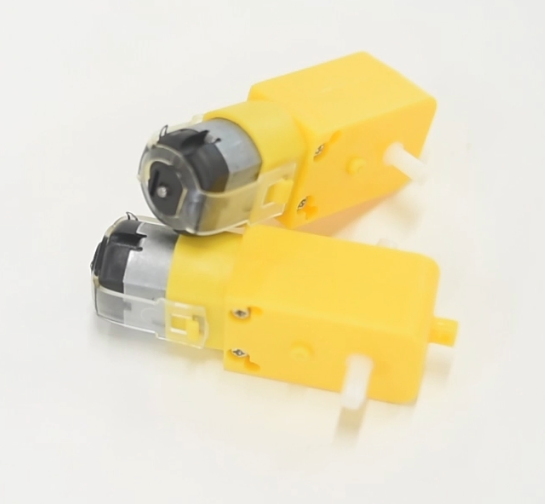
\includegraphics[width=0.5\columnwidth]{figs/motor.png}
\caption{DC motors}
\label{fig:motor}
\end{figure}

\begin{figure}[!ht]
\centering
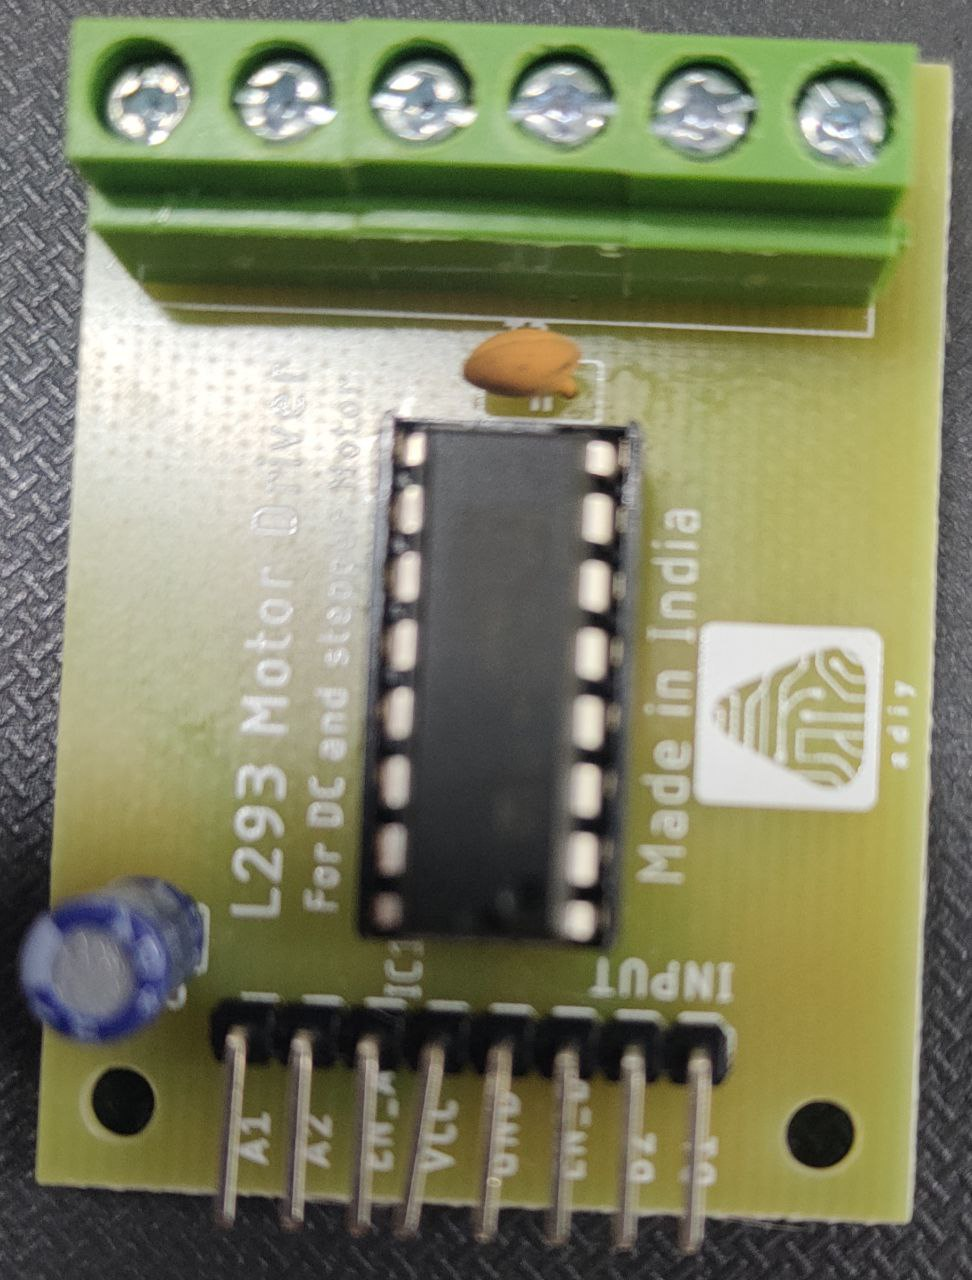
\includegraphics[width=0.3\columnwidth]{figs/driver.jpg}
\caption{L293 motor driver}
\label{fig:l293}
\end{figure}

\begin{figure}[!ht]
\centering
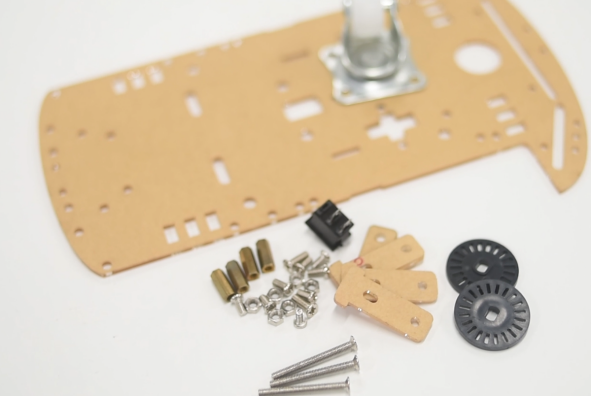
\includegraphics[width=0.5\columnwidth]{figs/base.png}
\caption{UGV frame/chassis}
\label{fig:frame}
\end{figure}

\begin{figure}[!ht]
\centering
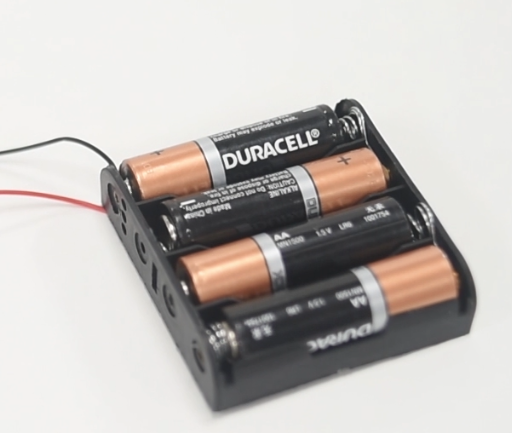
\includegraphics[width=0.5\columnwidth]{figs/battery.png}
\caption{Batteries for powering various equipments}
\label{fig:battery}
\end{figure}

\section{Assembling the UGV kit}

\item Assemble the Chassis using the provided nuts/screws, Wheels, and parts. 
 
 \begin{figure}[!ht]
\centering
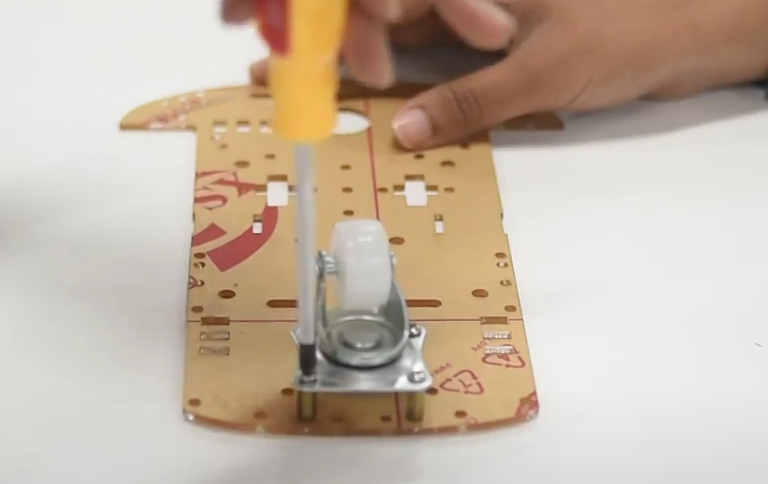
\includegraphics[width=0.3\columnwidth]{figs/2.png}
\centering
\caption{screws connecting }
\end{figure}
 
 \begin{figure}[!ht]
\centering
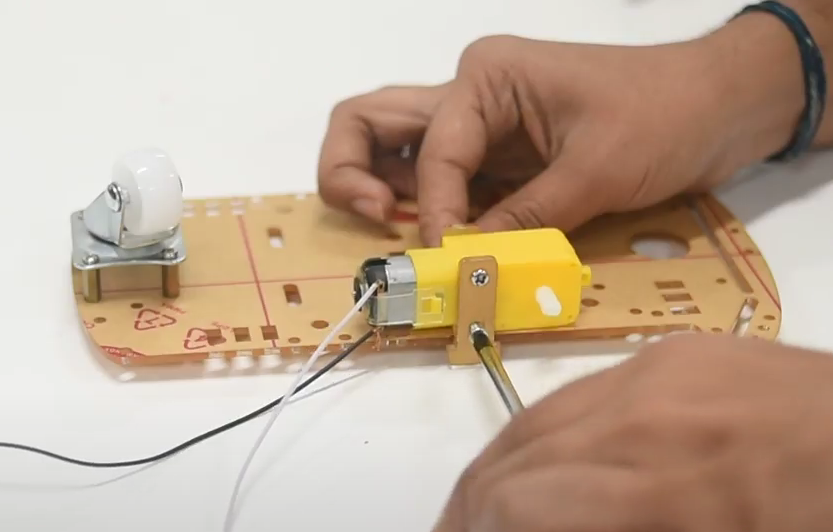
\includegraphics[width=0.3\columnwidth]{figs/3.png}
\caption{Dc motors connecting}
\end{figure}
 \begin{figure}[!ht]
\centering
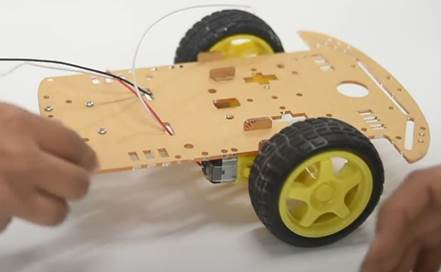
\includegraphics[width=0.3\columnwidth]{figs/6.jpg}
\caption{wheels connections }
\end{figure}
\section{Circuit Connections}

\begin{table}[!ht]
\centering
	%%%%%%%%%%%%%%%%%%%%%%%%%%%%%%%%%%%%%%%%%%%%%%%%%%%%%%%%%%%%%%%%%%%%%%
%%                                                                  %%
%%  This is the header of a LaTeX2e file exported from Gnumeric.    %%
%%                                                                  %%
%%  This file can be compiled as it stands or included in another   %%
%%  LaTeX document. The table is based on the longtable package so  %%
%%  the longtable options (headers, footers...) can be set in the   %%
%%  preamble section below (see PRAMBLE).                           %%
%%                                                                  %%
%%  To include the file in another, the following two lines must be %%
%%  in the including file:                                          %%
%%        \def\inputGnumericTable{}                                 %%
%%  at the beginning of the file and:                               %%
%%        \input{name-of-this-file.tex}                             %%
%%  where the table is to be placed. Note also that the including   %%
%%  file must use the following packages for the table to be        %%
%%  rendered correctly:                                             %%
%%    \usepackage[latin1]{inputenc}                                 %%
%%    \usepackage{color}                                            %%
%%    \usepackage{array}                                            %%
%%    \usepackage{longtable}                                        %%
%%    \usepackage{calc}                                             %%
%%    \usepackage{multirow}                                         %%
%%    \usepackage{hhline}                                           %%
%%    \usepackage{ifthen}                                           %%
%%  optionally (for landscape tables embedded in another document): %%
%%    \usepackage{lscape}                                           %%
%%                                                                  %%
%%%%%%%%%%%%%%%%%%%%%%%%%%%%%%%%%%%%%%%%%%%%%%%%%%%%%%%%%%%%%%%%%%%%%%



%%  This section checks if we are begin input into another file or  %%
%%  the file will be compiled alone. First use a macro taken from   %%
%%  the TeXbook ex 7.7 (suggestion of Han-Wen Nienhuys).            %%
\def\ifundefined#1{\expandafter\ifx\csname#1\endcsname\relax}


%%  Check for the \def token for inputed files. If it is not        %%
%%  defined, the file will be processed as a standalone and the     %%
%%  preamble will be used.                                          %%
\ifundefined{inputGnumericTable}

%%  We must be able to close or not the document at the end.        %%
	\def\gnumericTableEnd{\end{document}}


%%%%%%%%%%%%%%%%%%%%%%%%%%%%%%%%%%%%%%%%%%%%%%%%%%%%%%%%%%%%%%%%%%%%%%
%%                                                                  %%
%%  This is the PREAMBLE. Change these values to get the right      %%
%%  paper size and other niceties.                                  %%
%%                                                                  %%
%%%%%%%%%%%%%%%%%%%%%%%%%%%%%%%%%%%%%%%%%%%%%%%%%%%%%%%%%%%%%%%%%%%%%%

	\documentclass[12pt%
			  %,landscape%
                    ]{report}
       \usepackage[latin1]{inputenc}
       \usepackage{fullpage}
       \usepackage{color}
       \usepackage{array}
       \usepackage{longtable}
       \usepackage{calc}
       \usepackage{multirow}
       \usepackage{hhline}
       \usepackage{ifthen}

	\begin{document}


%%  End of the preamble for the standalone. The next section is for %%
%%  documents which are included into other LaTeX2e files.          %%
\else

%%  We are not a stand alone document. For a regular table, we will %%
%%  have no preamble and only define the closing to mean nothing.   %%
    \def\gnumericTableEnd{}

%%  If we want landscape mode in an embedded document, comment out  %%
%%  the line above and uncomment the two below. The table will      %%
%%  begin on a new page and run in landscape mode.                  %%
%       \def\gnumericTableEnd{\end{landscape}}
%       \begin{landscape}


%%  End of the else clause for this file being \input.              %%
\fi

%%%%%%%%%%%%%%%%%%%%%%%%%%%%%%%%%%%%%%%%%%%%%%%%%%%%%%%%%%%%%%%%%%%%%%
%%                                                                  %%
%%  The rest is the gnumeric table, except for the closing          %%
%%  statement. Changes below will alter the table's appearance.     %%
%%                                                                  %%
%%%%%%%%%%%%%%%%%%%%%%%%%%%%%%%%%%%%%%%%%%%%%%%%%%%%%%%%%%%%%%%%%%%%%%

\providecommand{\gnumericmathit}[1]{#1} 
%%  Uncomment the next line if you would like your numbers to be in %%
%%  italics if they are italizised in the gnumeric table.           %%
%\renewcommand{\gnumericmathit}[1]{\mathit{#1}}
\providecommand{\gnumericPB}[1]%
{\let\gnumericTemp=\\#1\let\\=\gnumericTemp\hspace{0pt}}
 \ifundefined{gnumericTableWidthDefined}
        \newlength{\gnumericTableWidth}
        \newlength{\gnumericTableWidthComplete}
        \newlength{\gnumericMultiRowLength}
        \global\def\gnumericTableWidthDefined{}
 \fi
%% The following setting protects this code from babel shorthands.  %%
 \ifthenelse{\isundefined{\languageshorthands}}{}{\languageshorthands{english}}
%%  The default table format retains the relative column widths of  %%
%%  gnumeric. They can easily be changed to c, r or l. In that case %%
%%  you may want to comment out the next line and uncomment the one %%
%%  thereafter                                                      %%
\providecommand\gnumbox{\makebox[0pt]}
%%\providecommand\gnumbox[1][]{\makebox}

%% to adjust positions in multirow situations                       %%
\setlength{\bigstrutjot}{\jot}
\setlength{\extrarowheight}{\doublerulesep}

%%  The \setlongtables command keeps column widths the same across  %%
%%  pages. Simply comment out next line for varying column widths.  %%
\setlongtables

\setlength\gnumericTableWidth{%
	125pt+%
	121pt+%
0pt}
\def\gumericNumCols{2}
\setlength\gnumericTableWidthComplete{\gnumericTableWidth+%
         \tabcolsep*\gumericNumCols*2+\arrayrulewidth*\gumericNumCols}
\ifthenelse{\lengthtest{\gnumericTableWidthComplete > \linewidth}}%
         {\def\gnumericScale{\ratio{\linewidth-%
                        \tabcolsep*\gumericNumCols*2-%
                        \arrayrulewidth*\gumericNumCols}%
{\gnumericTableWidth}}}%
{\def\gnumericScale{1}}

%%%%%%%%%%%%%%%%%%%%%%%%%%%%%%%%%%%%%%%%%%%%%%%%%%%%%%%%%%%%%%%%%%%%%%
%%                                                                  %%
%% The following are the widths of the various columns. We are      %%
%% defining them here because then they are easier to change.       %%
%% Depending on the cell formats we may use them more than once.    %%
%%                                                                  %%
%%%%%%%%%%%%%%%%%%%%%%%%%%%%%%%%%%%%%%%%%%%%%%%%%%%%%%%%%%%%%%%%%%%%%%

\ifthenelse{\isundefined{\gnumericColA}}{\newlength{\gnumericColA}}{}\settowidth{\gnumericColA}{\begin{tabular}{@{}p{125pt*\gnumericScale}@{}}x\end{tabular}}
\ifthenelse{\isundefined{\gnumericColB}}{\newlength{\gnumericColB}}{}\settowidth{\gnumericColB}{\begin{tabular}{@{}p{121pt*\gnumericScale}@{}}x\end{tabular}}

\begin{longtable}[c]{%
	b{\gnumericColA}%
	b{\gnumericColB}%
	}

%%%%%%%%%%%%%%%%%%%%%%%%%%%%%%%%%%%%%%%%%%%%%%%%%%%%%%%%%%%%%%%%%%%%%%
%%  The longtable options. (Caption, headers... see Goosens, p.124) %%
%	\caption{The Table Caption.}             \\	%
% \hline	% Across the top of the table.
%%  The rest of these options are table rows which are placed on    %%
%%  the first, last or every page. Use \multicolumn if you want.    %%

%%  Header for the first page.                                      %%
%	\multicolumn{2}{c}{The First Header} \\ \hline 
%	\multicolumn{1}{c}{colTag}	%Column 1
%	&\multicolumn{1}{c}{colTag}	\\ \hline %Last column
%	\endfirsthead

%%  The running header definition.                                  %%
%	\hline
%	\multicolumn{2}{l}{\ldots\small\slshape continued} \\ \hline
%	\multicolumn{1}{c}{colTag}	%Column 1
%	&\multicolumn{1}{c}{colTag}	\\ \hline %Last column
%	\endhead

%%  The running footer definition.                                  %%
%	\hline
%	\multicolumn{2}{r}{\small\slshape continued\ldots} \\
%	\endfoot

%%  The ending footer definition.                                   %%
%	\multicolumn{2}{c}{That's all folks} \\ \hline 
%	\endlastfoot
%%%%%%%%%%%%%%%%%%%%%%%%%%%%%%%%%%%%%%%%%%%%%%%%%%%%%%%%%%%%%%%%%%%%%%

\hhline{|-|-}
	 \multicolumn{1}{|p{\gnumericColA}|}%
	{\gnumericPB{\raggedright}\gnumbox[l]{\textbf{Motor Driver Unit}}}
	&\multicolumn{1}{p{\gnumericColB}|}%
	{\gnumericPB{\raggedright}\gnumbox[l]{\textbf{DC Motor}}}
\\
\hhline{|--|}
	 \multicolumn{1}{|p{\gnumericColA}|}%
	{\gnumericPB{\raggedright}\gnumbox[l]{MA1}}
	&\multicolumn{1}{p{\gnumericColB}|}%
	{\gnumericPB{\raggedright}\gnumbox[l]{Right Motor Input 1}}
\\
\hhline{|--|}
	 \multicolumn{1}{|p{\gnumericColA}|}%
	{\gnumericPB{\raggedright}\gnumbox[l]{MA2}}
	&\multicolumn{1}{p{\gnumericColB}|}%
	{\gnumericPB{\raggedright}\gnumbox[l]{Right Motor Input 2}}
\\
\hhline{|--|}
	 \multicolumn{1}{|p{\gnumericColA}|}%
	{\gnumericPB{\raggedright}\gnumbox[l]{MB1}}
	&\multicolumn{1}{p{\gnumericColB}|}%
	{\gnumericPB{\raggedright}\gnumbox[l]{Left Motor Input 1}}
\\
\hhline{|--|}
	 \multicolumn{1}{|p{\gnumericColA}|}%
	{\gnumericPB{\raggedright}\gnumbox[l]{MB2}}
	&\multicolumn{1}{p{\gnumericColB}|}%
	{\gnumericPB{\raggedright}\gnumbox[l]{Left Motor Input 2}}
\\
\hhline{|--|}
	 \multicolumn{1}{|p{\gnumericColA}|}%
	{\gnumericPB{\raggedright}\gnumbox[l]{5v}}
	&\multicolumn{1}{p{\gnumericColB}|}%
	{\gnumericPB{\raggedright}\gnumbox[l]{VCC}}
\\
\hhline{|--|}
	 \multicolumn{1}{|p{\gnumericColA}|}%
	{\gnumericPB{\raggedright}\gnumbox[l]{GND}}
	&\multicolumn{1}{p{\gnumericColB}|}%
	{\gnumericPB{\raggedright}\gnumbox[l]{GND}}
\\
\hhline{|-|-|}
\end{longtable}

\ifthenelse{\isundefined{\languageshorthands}}{}{\languageshorthands{\languagename}}
\gnumericTableEnd

	\caption{DC motor connection with L293 Motor Driver }
	\label{Tab:dcmotor}
\end{table}
%\item  Make the Circuit Connections as per the  \tabref{Tab:dcmotor}

\begin{table}[!ht]
\centering
	%%%%%%%%%%%%%%%%%%%%%%%%%%%%%%%%%%%%%%%%%%%%%%%%%%%%%%%%%%%%%%%%%%%%%%
%%                                                                  %%
%%  This is the header of a LaTeX2e file exported from Gnumeric.    %%
%%                                                                  %%
%%  This file can be compiled as it stands or included in another   %%
%%  LaTeX document. The table is based on the longtable package so  %%
%%  the longtable options (headers, footers...) can be set in the   %%
%%  preamble section below (see PRAMBLE).                           %%
%%                                                                  %%
%%  To include the file in another, the following two lines must be %%
%%  in the including file:                                          %%
%%        \def\inputGnumericTable{}                                 %%
%%  at the beginning of the file and:                               %%
%%        \input{name-of-this-file.tex}                             %%
%%  where the table is to be placed. Note also that the including   %%
%%  file must use the following packages for the table to be        %%
%%  rendered correctly:                                             %%
%%    \usepackage[latin1]{inputenc}                                 %%
%%    \usepackage{color}                                            %%
%%    \usepackage{array}                                            %%
%%    \usepackage{longtable}                                        %%
%%    \usepackage{calc}                                             %%
%%    \usepackage{multirow}                                         %%
%%    \usepackage{hhline}                                           %%
%%    \usepackage{ifthen}                                           %%
%%  optionally (for landscape tables embedded in another document): %%
%%    \usepackage{lscape}                                           %%
%%                                                                  %%
%%%%%%%%%%%%%%%%%%%%%%%%%%%%%%%%%%%%%%%%%%%%%%%%%%%%%%%%%%%%%%%%%%%%%%



%%  This section checks if we are begin input into another file or  %%
%%  the file will be compiled alone. First use a macro taken from   %%
%%  the TeXbook ex 7.7 (suggestion of Han-Wen Nienhuys).            %%
\def\ifundefined#1{\expandafter\ifx\csname#1\endcsname\relax}


%%  Check for the \def token for inputed files. If it is not        %%
%%  defined, the file will be processed as a standalone and the     %%
%%  preamble will be used.                                          %%
\ifundefined{inputGnumericTable}

%%  We must be able to close or not the document at the end.        %%
	\def\gnumericTableEnd{\end{document}}


%%%%%%%%%%%%%%%%%%%%%%%%%%%%%%%%%%%%%%%%%%%%%%%%%%%%%%%%%%%%%%%%%%%%%%
%%                                                                  %%
%%  This is the PREAMBLE. Change these values to get the right      %%
%%  paper size and other niceties.                                  %%
%%                                                                  %%
%%%%%%%%%%%%%%%%%%%%%%%%%%%%%%%%%%%%%%%%%%%%%%%%%%%%%%%%%%%%%%%%%%%%%%

	\documentclass[12pt%
			  %,landscape%
                    ]{report}
       \usepackage[latin1]{inputenc}
       \usepackage{fullpage}
       \usepackage{color}
       \usepackage{array}
       \usepackage{longtable}
       \usepackage{calc}
       \usepackage{multirow}
       \usepackage{hhline}
       \usepackage{ifthen}

	\begin{document}


%%  End of the preamble for the standalone. The next section is for %%
%%  documents which are included into other LaTeX2e files.          %%
\else

%%  We are not a stand alone document. For a regular table, we will %%
%%  have no preamble and only define the closing to mean nothing.   %%
    \def\gnumericTableEnd{}

%%  If we want landscape mode in an embedded document, comment out  %%
%%  the line above and uncomment the two below. The table will      %%
%%  begin on a new page and run in landscape mode.                  %%
%       \def\gnumericTableEnd{\end{landscape}}
%       \begin{landscape}


%%  End of the else clause for this file being \input.              %%
\fi

%%%%%%%%%%%%%%%%%%%%%%%%%%%%%%%%%%%%%%%%%%%%%%%%%%%%%%%%%%%%%%%%%%%%%%
%%                                                                  %%
%%  The rest is the gnumeric table, except for the closing          %%
%%  statement. Changes below will alter the table's appearance.     %%
%%                                                                  %%
%%%%%%%%%%%%%%%%%%%%%%%%%%%%%%%%%%%%%%%%%%%%%%%%%%%%%%%%%%%%%%%%%%%%%%

\providecommand{\gnumericmathit}[1]{#1} 
%%  Uncomment the next line if you would like your numbers to be in %%
%%  italics if they are italizised in the gnumeric table.           %%
%\renewcommand{\gnumericmathit}[1]{\mathit{#1}}
\providecommand{\gnumericPB}[1]%
{\let\gnumericTemp=\\#1\let\\=\gnumericTemp\hspace{0pt}}
 \ifundefined{gnumericTableWidthDefined}
        \newlength{\gnumericTableWidth}
        \newlength{\gnumericTableWidthComplete}
        \newlength{\gnumericMultiRowLength}
        \global\def\gnumericTableWidthDefined{}
 \fi
%% The following setting protects this code from babel shorthands.  %%
 \ifthenelse{\isundefined{\languageshorthands}}{}{\languageshorthands{english}}
%%  The default table format retains the relative column widths of  %%
%%  gnumeric. They can easily be changed to c, r or l. In that case %%
%%  you may want to comment out the next line and uncomment the one %%
%%  thereafter                                                      %%
\providecommand\gnumbox{\makebox[0pt]}
%%\providecommand\gnumbox[1][]{\makebox}

%% to adjust positions in multirow situations                       %%
\setlength{\bigstrutjot}{\jot}
\setlength{\extrarowheight}{\doublerulesep}

%%  The \setlongtables command keeps column widths the same across  %%
%%  pages. Simply comment out next line for varying column widths.  %%
\setlongtables

\setlength\gnumericTableWidth{%
	125pt+%
	121pt+%
0pt}
\def\gumericNumCols{2}
\setlength\gnumericTableWidthComplete{\gnumericTableWidth+%
         \tabcolsep*\gumericNumCols*2+\arrayrulewidth*\gumericNumCols}
\ifthenelse{\lengthtest{\gnumericTableWidthComplete > \linewidth}}%
         {\def\gnumericScale{\ratio{\linewidth-%
                        \tabcolsep*\gumericNumCols*2-%
                        \arrayrulewidth*\gumericNumCols}%
{\gnumericTableWidth}}}%
{\def\gnumericScale{1}}

%%%%%%%%%%%%%%%%%%%%%%%%%%%%%%%%%%%%%%%%%%%%%%%%%%%%%%%%%%%%%%%%%%%%%%
%%                                                                  %%
%% The following are the widths of the various columns. We are      %%
%% defining them here because then they are easier to change.       %%
%% Depending on the cell formats we may use them more than once.    %%
%%                                                                  %%
%%%%%%%%%%%%%%%%%%%%%%%%%%%%%%%%%%%%%%%%%%%%%%%%%%%%%%%%%%%%%%%%%%%%%%

\ifthenelse{\isundefined{\gnumericColA}}{\newlength{\gnumericColA}}{}\settowidth{\gnumericColA}{\begin{tabular}{@{}p{125pt*\gnumericScale}@{}}x\end{tabular}}
\ifthenelse{\isundefined{\gnumericColB}}{\newlength{\gnumericColB}}{}\settowidth{\gnumericColB}{\begin{tabular}{@{}p{121pt*\gnumericScale}@{}}x\end{tabular}}

\begin{longtable}[c]{%
	b{\gnumericColA}%
	b{\gnumericColB}%
	}

%%%%%%%%%%%%%%%%%%%%%%%%%%%%%%%%%%%%%%%%%%%%%%%%%%%%%%%%%%%%%%%%%%%%%%
%%  The longtable options. (Caption, headers... see Goosens, p.124) %%
%	\caption{The Table Caption.}             \\	%
% \hline	% Across the top of the table.
%%  The rest of these options are table rows which are placed on    %%
%%  the first, last or every page. Use \multicolumn if you want.    %%

%%  Header for the first page.                                      %%
%	\multicolumn{2}{c}{The First Header} \\ \hline 
%	\multicolumn{1}{c}{colTag}	%Column 1
%	&\multicolumn{1}{c}{colTag}	\\ \hline %Last column
%	\endfirsthead

%%  The running header definition.                                  %%
%	\hline
%	\multicolumn{2}{l}{\ldots\small\slshape continued} \\ \hline
%	\multicolumn{1}{c}{colTag}	%Column 1
%	&\multicolumn{1}{c}{colTag}	\\ \hline %Last column
%	\endhead

%%  The running footer definition.                                  %%
%	\hline
%	\multicolumn{2}{r}{\small\slshape continued\ldots} \\
%	\endfoot

%%  The ending footer definition.                                   %%
%	\multicolumn{2}{c}{That's all folks} \\ \hline 
%	\endlastfoot
%%%%%%%%%%%%%%%%%%%%%%%%%%%%%%%%%%%%%%%%%%%%%%%%%%%%%%%%%%%%%%%%%%%%%%

\hhline{|-|-}
	 \multicolumn{1}{|p{\gnumericColA}|}%
	{\gnumericPB{\raggedright}\gnumbox[l]{\textbf{Vaman Board ESP 32}}}
	&\multicolumn{1}{p{\gnumericColB}|}%
	{\gnumericPB{\raggedright}\gnumbox[l]{\textbf{Motor Driver Unit}}}
\\
\hhline{|--|}
	 \multicolumn{1}{|p{\gnumericColA}|}%
	{\gnumericPB{\raggedright}\gnumbox[l]{Pin 16}}
	&\multicolumn{1}{p{\gnumericColB}|}%
	{\gnumericPB{\raggedright}\gnumbox[l]{ Input A1}}
\\
\hhline{|--|}
	 \multicolumn{1}{|p{\gnumericColA}|}%
	{\gnumericPB{\raggedright}\gnumbox[l]{Pin 17}}
	&\multicolumn{1}{p{\gnumericColB}|}%
	{\gnumericPB{\raggedright}\gnumbox[l]{ Input  A2}}
\\
\hhline{|--|}
	 \multicolumn{1}{|p{\gnumericColA}|}%
	{\gnumericPB{\raggedright}\gnumbox[l]{Pin 18}}
	&\multicolumn{1}{p{\gnumericColB}|}%
	{\gnumericPB{\raggedright}\gnumbox[l]{ Input B1}}
\\
\hhline{|--|}
	 \multicolumn{1}{|p{\gnumericColA}|}%
	{\gnumericPB{\raggedright}\gnumbox[l]{Pin 19}}
	&\multicolumn{1}{p{\gnumericColB}|}%
	{\gnumericPB{\raggedright}\gnumbox[l]{ Input B2}}
\\
\hhline{|--|}
	 \multicolumn{1}{|p{\gnumericColA}|}%
	{\gnumericPB{\raggedright}\gnumbox[l]{5v}}
	&\multicolumn{1}{p{\gnumericColB}|}%
	{\gnumericPB{\raggedright}\gnumbox[l]{VCC}}
\\
\hhline{|--|}
	 \multicolumn{1}{|p{\gnumericColA}|}%
	{\gnumericPB{\raggedright}\gnumbox[l]{GND}}
	&\multicolumn{1}{p{\gnumericColB}|}%
	{\gnumericPB{\raggedright}\gnumbox[l]{GND}}
\\
\hhline{|-|-|}
\end{longtable}

\ifthenelse{\isundefined{\languageshorthands}}{}{\languageshorthands{\languagename}}
\gnumericTableEnd

	\caption{ vaman Connections}
	\label{Tab:connections3}
\end{table}
%\item Make the Circuit Connections as per the \tabref{Tab:connections3}.
\item Connect the Arduino-UART pins to the Vaman ESP32 pins according to \tabref{tab:arduino-uart}.
\item For Bluetooth toycar connect the circuits connection as per \tabref{Tab:dcmotor} and  \tabref{Tab:connections3}.
\begin{table}[!ht]
\centering
	%%%%%%%%%%%%%%%%%%%%%%%%%%%%%%%%%%%%%%%%%%%%%%%%%%%%%%%%%%%%%%%%%%%%%%
%%                                                                  %%
%%  This is the header of a LaTeX2e file exported from Gnumeric.    %%
%%                                                                  %%
%%  This file can be compiled as it stands or included in another   %%
%%  LaTeX document. The table is based on the longtable package so  %%
%%  the longtable options (headers, footers...) can be set in the   %%
%%  preamble section below (see PRAMBLE).                           %%
%%                                                                  %%
%%  To include the file in another, the following two lines must be %%
%%  in the including file:                                          %%
%%        \def\inputGnumericTable{}                                 %%
%%  at the beginning of the file and:                               %%
%%        \input{name-of-this-file.tex}                             %%
%%  where the table is to be placed. Note also that the including   %%
%%  file must use the following packages for the table to be        %%
%%  rendered correctly:                                             %%
%%    \usepackage[latin1]{inputenc}                                 %%
%%    \usepackage{color}                                            %%
%%    \usepackage{array}                                            %%
%%    \usepackage{longtable}                                        %%
%%    \usepackage{calc}                                             %%
%%    \usepackage{multirow}                                         %%
%%    \usepackage{hhline}                                           %%
%%    \usepackage{ifthen}                                           %%
%%  optionally (for landscape tables embedded in another document): %%
%%    \usepackage{lscape}                                           %%
%%                                                                  %%
%%%%%%%%%%%%%%%%%%%%%%%%%%%%%%%%%%%%%%%%%%%%%%%%%%%%%%%%%%%%%%%%%%%%%%



%%  This section checks if we are begin input into another file or  %%
%%  the file will be compiled alone. First use a macro taken from   %%
%%  the TeXbook ex 7.7 (suggestion of Han-Wen Nienhuys).            %%
\def\ifundefined#1{\expandafter\ifx\csname#1\endcsname\relax}


%%  Check for the \def token for inputed files. If it is not        %%
%%  defined, the file will be processed as a standalone and the     %%
%%  preamble will be used.                                          %%
\ifundefined{inputGnumericTable}

%%  We must be able to close or not the document at the end.        %%
	\def\gnumericTableEnd{\end{document}}


%%%%%%%%%%%%%%%%%%%%%%%%%%%%%%%%%%%%%%%%%%%%%%%%%%%%%%%%%%%%%%%%%%%%%%
%%                                                                  %%
%%  This is the PREAMBLE. Change these values to get the right      %%
%%  paper size and other niceties.                                  %%
%%                                                                  %%
%%%%%%%%%%%%%%%%%%%%%%%%%%%%%%%%%%%%%%%%%%%%%%%%%%%%%%%%%%%%%%%%%%%%%%

	\documentclass[12pt%
			  %,landscape%
                    ]{report}
       \usepackage[latin1]{inputenc}
       \usepackage{fullpage}
       \usepackage{color}
       \usepackage{array}
       \usepackage{longtable}
       \usepackage{calc}
       \usepackage{multirow}
       \usepackage{hhline}
       \usepackage{ifthen}

	\begin{document}


%%  End of the preamble for the standalone. The next section is for %%
%%  documents which are included into other LaTeX2e files.          %%
\else

%%  We are not a stand alone document. For a regular table, we will %%
%%  have no preamble and only define the closing to mean nothing.   %%
    \def\gnumericTableEnd{}

%%  If we want landscape mode in an embedded document, comment out  %%
%%  the line above and uncomment the two below. The table will      %%
%%  begin on a new page and run in landscape mode.                  %%
%       \def\gnumericTableEnd{\end{landscape}}
%       \begin{landscape}


%%  End of the else clause for this file being \input.              %%
\fi

%%%%%%%%%%%%%%%%%%%%%%%%%%%%%%%%%%%%%%%%%%%%%%%%%%%%%%%%%%%%%%%%%%%%%%
%%                                                                  %%
%%  The rest is the gnumeric table, except for the closing          %%
%%  statement. Changes below will alter the table's appearance.     %%
%%                                                                  %%
%%%%%%%%%%%%%%%%%%%%%%%%%%%%%%%%%%%%%%%%%%%%%%%%%%%%%%%%%%%%%%%%%%%%%%

\providecommand{\gnumericmathit}[1]{#1} 
%%  Uncomment the next line if you would like your numbers to be in %%
%%  italics if they are italizised in the gnumeric table.           %%
%\renewcommand{\gnumericmathit}[1]{\mathit{#1}}
\providecommand{\gnumericPB}[1]%
{\let\gnumericTemp=\\#1\let\\=\gnumericTemp\hspace{0pt}}
 \ifundefined{gnumericTableWidthDefined}
        \newlength{\gnumericTableWidth}
        \newlength{\gnumericTableWidthComplete}
        \newlength{\gnumericMultiRowLength}
        \global\def\gnumericTableWidthDefined{}
 \fi
%% The following setting protects this code from babel shorthands.  %%
 \ifthenelse{\isundefined{\languageshorthands}}{}{\languageshorthands{english}}
%%  The default table format retains the relative column widths of  %%
%%  gnumeric. They can easily be changed to c, r or l. In that case %%
%%  you may want to comment out the next line and uncomment the one %%
%%  thereafter                                                      %%
\providecommand\gnumbox{\makebox[0pt]}
%%\providecommand\gnumbox[1][]{\makebox}

%% to adjust positions in multirow situations                       %%
\setlength{\bigstrutjot}{\jot}
\setlength{\extrarowheight}{\doublerulesep}

%%  The \setlongtables command keeps column widths the same across  %%
%%  pages. Simply comment out next line for varying column widths.  %%
\setlongtables

\setlength\gnumericTableWidth{%
	125pt+%
	121pt+%
0pt}
\def\gumericNumCols{2}
\setlength\gnumericTableWidthComplete{\gnumericTableWidth+%
         \tabcolsep*\gumericNumCols*2+\arrayrulewidth*\gumericNumCols}
\ifthenelse{\lengthtest{\gnumericTableWidthComplete > \linewidth}}%
         {\def\gnumericScale{\ratio{\linewidth-%
                        \tabcolsep*\gumericNumCols*2-%
                        \arrayrulewidth*\gumericNumCols}%
{\gnumericTableWidth}}}%
{\def\gnumericScale{1}}

%%%%%%%%%%%%%%%%%%%%%%%%%%%%%%%%%%%%%%%%%%%%%%%%%%%%%%%%%%%%%%%%%%%%%%
%%                                                                  %%
%% The following are the widths of the various columns. We are      %%
%% defining them here because then they are easier to change.       %%
%% Depending on the cell formats we may use them more than once.    %%
%%                                                                  %%
%%%%%%%%%%%%%%%%%%%%%%%%%%%%%%%%%%%%%%%%%%%%%%%%%%%%%%%%%%%%%%%%%%%%%%

\ifthenelse{\isundefined{\gnumericColA}}{\newlength{\gnumericColA}}{}\settowidth{\gnumericColA}{\begin{tabular}{@{}p{125pt*\gnumericScale}@{}}x\end{tabular}}
\ifthenelse{\isundefined{\gnumericColB}}{\newlength{\gnumericColB}}{}\settowidth{\gnumericColB}{\begin{tabular}{@{}p{121pt*\gnumericScale}@{}}x\end{tabular}}

\begin{longtable}[c]{%
	b{\gnumericColA}%
	b{\gnumericColB}%
	}

%%%%%%%%%%%%%%%%%%%%%%%%%%%%%%%%%%%%%%%%%%%%%%%%%%%%%%%%%%%%%%%%%%%%%%
%%  The longtable options. (Caption, headers... see Goosens, p.124) %%
%	\caption{The Table Caption.}             \\	%
% \hline	% Across the top of the table.
%%  The rest of these options are table rows which are placed on    %%
%%  the first, last or every page. Use \multicolumn if you want.    %%

%%  Header for the first page.                                      %%
%	\multicolumn{2}{c}{The First Header} \\ \hline 
%	\multicolumn{1}{c}{colTag}	%Column 1
%	&\multicolumn{1}{c}{colTag}	\\ \hline %Last column
%	\endfirsthead

%%  The running header definition.                                  %%
%	\hline
%	\multicolumn{2}{l}{\ldots\small\slshape continued} \\ \hline
%	\multicolumn{1}{c}{colTag}	%Column 1
%	&\multicolumn{1}{c}{colTag}	\\ \hline %Last column
%	\endhead

%%  The running footer definition.                                  %%
%	\hline
%	\multicolumn{2}{r}{\small\slshape continued\ldots} \\
%	\endfoot

%%  The ending footer definition.                                   %%
%	\multicolumn{2}{c}{That's all folks} \\ \hline 
%	\endlastfoot
%%%%%%%%%%%%%%%%%%%%%%%%%%%%%%%%%%%%%%%%%%%%%%%%%%%%%%%%%%%%%%%%%%%%%%

\hhline{|-|-}
	 \multicolumn{1}{|p{\gnumericColA}|}%
	{\gnumericPB{\raggedright}\gnumbox[l]{\textbf{Vaman Board}}}
	&\multicolumn{1}{p{\gnumericColB}|}%
	{\gnumericPB{\raggedright}\gnumbox[l]{\textbf{Motor Driver Unit}}}
\\
\hhline{|--|}
	 \multicolumn{1}{|p{\gnumericColA}|}%
	{\gnumericPB{\raggedright}\gnumbox[l]{Pin 21}}
	&\multicolumn{1}{p{\gnumericColB}|}%
	{\gnumericPB{\raggedright}\gnumbox[l]{Right Motor Input 1}}
\\
\hhline{|--|}
	 \multicolumn{1}{|p{\gnumericColA}|}%
	{\gnumericPB{\raggedright}\gnumbox[l]{Pin 18}}
	&\multicolumn{1}{p{\gnumericColB}|}%
	{\gnumericPB{\raggedright}\gnumbox[l]{Right Motor Input 2}}
\\
\hhline{|--|}
	 \multicolumn{1}{|p{\gnumericColA}|}%
	{\gnumericPB{\raggedright}\gnumbox[l]{Pin 23}}
	&\multicolumn{1}{p{\gnumericColB}|}%
	{\gnumericPB{\raggedright}\gnumbox[l]{Left Motor Input 1}}
\\
\hhline{|--|}
	 \multicolumn{1}{|p{\gnumericColA}|}%
	{\gnumericPB{\raggedright}\gnumbox[l]{Pin 22}}
	&\multicolumn{1}{p{\gnumericColB}|}%
	{\gnumericPB{\raggedright}\gnumbox[l]{Left Motor Input 2}}
\\
\hhline{|--|}
	 \multicolumn{1}{|p{\gnumericColA}|}%
	{\gnumericPB{\raggedright}\gnumbox[l]{5v}}
	&\multicolumn{1}{p{\gnumericColB}|}%
	{\gnumericPB{\raggedright}\gnumbox[l]{VCC}}
\\
\hhline{|--|}
	 \multicolumn{1}{|p{\gnumericColA}|}%
	{\gnumericPB{\raggedright}\gnumbox[l]{GND}}
	&\multicolumn{1}{p{\gnumericColB}|}%
	{\gnumericPB{\raggedright}\gnumbox[l]{GND}}
\\
\hhline{|-|-|}
\end{longtable}

\ifthenelse{\isundefined{\languageshorthands}}{}{\languageshorthands{\languagename}}
\gnumericTableEnd

	\caption{connection with vaman board }
	\label{Tab:connections}
\end{table}
\begin{table}[!ht]
%\item Make the Motor Driver Connections as per the \tabref{Tab:connections}
\centering
	%%%%%%%%%%%%%%%%%%%%%%%%%%%%%%%%%%%%%%%%%%%%%%%%%%%%%%%%%%%%%%%%%%%%%%
%%                                                                  %%
%%  This is the header of a LaTeX2e file exported from Gnumeric.    %%
%%                                                                  %%
%%  This file can be compiled as it stands or included in another   %%
%%  LaTeX document. The table is based on the longtable package so  %%
%%  the longtable options (headers, footers...) can be set in the   %%
%%  preamble section below (see PRAMBLE).                           %%
%%                                                                  %%
%%  To include the file in another, the following two lines must be %%
%%  in the including file:                                          %%
%%        \def\inputGnumericTable{}                                 %%
%%  at the beginning of the file and:                               %%
%%        \input{name-of-this-file.tex}                             %%
%%  where the table is to be placed. Note also that the including   %%
%%  file must use the following packages for the table to be        %%
%%  rendered correctly:                                             %%
%%    \usepackage[latin1]{inputenc}                                 %%
%%    \usepackage{color}                                            %%
%%    \usepackage{array}                                            %%
%%    \usepackage{longtable}                                        %%
%%    \usepackage{calc}                                             %%
%%    \usepackage{multirow}                                         %%
%%    \usepackage{hhline}                                           %%
%%    \usepackage{ifthen}                                           %%
%%  optionally (for landscape tables embedded in another document): %%
%%    \usepackage{lscape}                                           %%
%%                                                                  %%
%%%%%%%%%%%%%%%%%%%%%%%%%%%%%%%%%%%%%%%%%%%%%%%%%%%%%%%%%%%%%%%%%%%%%%



%%  This section checks if we are begin input into another file or  %%
%%  the file will be compiled alone. First use a macro taken from   %%
%%  the TeXbook ex 7.7 (suggestion of Han-Wen Nienhuys).            %%
\def\ifundefined#1{\expandafter\ifx\csname#1\endcsname\relax}


%%  Check for the \def token for inputed files. If it is not        %%
%%  defined, the file will be processed as a standalone and the     %%
%%  preamble will be used.                                          %%
\ifundefined{inputGnumericTable}

%%  We must be able to close or not the document at the end.        %%
	\def\gnumericTableEnd{\end{document}}


%%%%%%%%%%%%%%%%%%%%%%%%%%%%%%%%%%%%%%%%%%%%%%%%%%%%%%%%%%%%%%%%%%%%%%
%%                                                                  %%
%%  This is the PREAMBLE. Change these values to get the right      %%
%%  paper size and other niceties.                                  %%
%%                                                                  %%
%%%%%%%%%%%%%%%%%%%%%%%%%%%%%%%%%%%%%%%%%%%%%%%%%%%%%%%%%%%%%%%%%%%%%%

	\documentclass[12pt%
			  %,landscape%
                    ]{report}
       \usepackage[latin1]{inputenc}
       \usepackage{fullpage}
       \usepackage{color}
       \usepackage{array}
       \usepackage{longtable}
       \usepackage{calc}
       \usepackage{multirow}
       \usepackage{hhline}
       \usepackage{ifthen}

	\begin{document}


%%  End of the preamble for the standalone. The next section is for %%
%%  documents which are included into other LaTeX2e files.          %%
\else

%%  We are not a stand alone document. For a regular table, we will %%
%%  have no preamble and only define the closing to mean nothing.   %%
    \def\gnumericTableEnd{}

%%  If we want landscape mode in an embedded document, comment out  %%
%%  the line above and uncomment the two below. The table will      %%
%%  begin on a new page and run in landscape mode.                  %%
%       \def\gnumericTableEnd{\end{landscape}}
%       \begin{landscape}


%%  End of the else clause for this file being \input.              %%
\fi

%%%%%%%%%%%%%%%%%%%%%%%%%%%%%%%%%%%%%%%%%%%%%%%%%%%%%%%%%%%%%%%%%%%%%%
%%                                                                  %%
%%  The rest is the gnumeric table, except for the closing          %%
%%  statement. Changes below will alter the table's appearance.     %%
%%                                                                  %%
%%%%%%%%%%%%%%%%%%%%%%%%%%%%%%%%%%%%%%%%%%%%%%%%%%%%%%%%%%%%%%%%%%%%%%

\providecommand{\gnumericmathit}[1]{#1} 
%%  Uncomment the next line if you would like your numbers to be in %%
%%  italics if they are italizised in the gnumeric table.           %%
%\renewcommand{\gnumericmathit}[1]{\mathit{#1}}
\providecommand{\gnumericPB}[1]%
{\let\gnumericTemp=\\#1\let\\=\gnumericTemp\hspace{0pt}}
 \ifundefined{gnumericTableWidthDefined}
        \newlength{\gnumericTableWidth}
        \newlength{\gnumericTableWidthComplete}
        \newlength{\gnumericMultiRowLength}
        \global\def\gnumericTableWidthDefined{}
 \fi
%% The following setting protects this code from babel shorthands.  %%
 \ifthenelse{\isundefined{\languageshorthands}}{}{\languageshorthands{english}}
%%  The default table format retains the relative column widths of  %%
%%  gnumeric. They can easily be changed to c, r or l. In that case %%
%%  you may want to comment out the next line and uncomment the one %%
%%  thereafter                                                      %%
\providecommand\gnumbox{\makebox[0pt]}
%%\providecommand\gnumbox[1][]{\makebox}

%% to adjust positions in multirow situations                       %%
\setlength{\bigstrutjot}{\jot}
\setlength{\extrarowheight}{\doublerulesep}

%%  The \setlongtables command keeps column widths the same across  %%
%%  pages. Simply comment out next line for varying column widths.  %%
\setlongtables

\setlength\gnumericTableWidth{%
	53pt+%
	105pt+%
	65pt+%
	70pt+%
0pt}
\def\gumericNumCols{4}
\setlength\gnumericTableWidthComplete{\gnumericTableWidth+%
         \tabcolsep*\gumericNumCols*2+\arrayrulewidth*\gumericNumCols}
\ifthenelse{\lengthtest{\gnumericTableWidthComplete > \linewidth}}%
         {\def\gnumericScale{\ratio{\linewidth-%
                        \tabcolsep*\gumericNumCols*2-%
                        \arrayrulewidth*\gumericNumCols}%
{\gnumericTableWidth}}}%
{\def\gnumericScale{1}}

%%%%%%%%%%%%%%%%%%%%%%%%%%%%%%%%%%%%%%%%%%%%%%%%%%%%%%%%%%%%%%%%%%%%%%
%%                                                                  %%
%% The following are the widths of the various columns. We are      %%
%% defining them here because then they are easier to change.       %%
%% Depending on the cell formats we may use them more than once.    %%
%%                                                                  %%
%%%%%%%%%%%%%%%%%%%%%%%%%%%%%%%%%%%%%%%%%%%%%%%%%%%%%%%%%%%%%%%%%%%%%%

\ifthenelse{\isundefined{\gnumericColA}}{\newlength{\gnumericColA}}{}\settowidth{\gnumericColA}{\begin{tabular}{@{}p{53pt*\gnumericScale}@{}}x\end{tabular}}
\ifthenelse{\isundefined{\gnumericColB}}{\newlength{\gnumericColB}}{}\settowidth{\gnumericColB}{\begin{tabular}{@{}p{105pt*\gnumericScale}@{}}x\end{tabular}}
\ifthenelse{\isundefined{\gnumericColC}}{\newlength{\gnumericColC}}{}\settowidth{\gnumericColC}{\begin{tabular}{@{}p{65pt*\gnumericScale}@{}}x\end{tabular}}
\ifthenelse{\isundefined{\gnumericColD}}{\newlength{\gnumericColD}}{}\settowidth{\gnumericColD}{\begin{tabular}{@{}p{70pt*\gnumericScale}@{}}x\end{tabular}}

\begin{longtable}[c]{%
	b{\gnumericColA}%
	b{\gnumericColB}%
	b{\gnumericColC}%
	b{\gnumericColD}%
	}

%%%%%%%%%%%%%%%%%%%%%%%%%%%%%%%%%%%%%%%%%%%%%%%%%%%%%%%%%%%%%%%%%%%%%%
%%  The longtable options. (Caption, headers... see Goosens, p.124) %%
%	\caption{The Table Caption.}             \\	%
% \hline	% Across the top of the table.
%%  The rest of these options are table rows which are placed on    %%
%%  the first, last or every page. Use \multicolumn if you want.    %%

%%  Header for the first page.                                      %%
%	\multicolumn{4}{c}{The First Header} \\ \hline 
%	\multicolumn{1}{c}{colTag}	%Column 1
%	&\multicolumn{1}{c}{colTag}	%Column 2
%	&\multicolumn{1}{c}{colTag}	%Column 3
%	&\multicolumn{1}{c}{colTag}	\\ \hline %Last column
%	\endfirsthead

%%  The running header definition.                                  %%
%	\hline
%	\multicolumn{4}{l}{\ldots\small\slshape continued} \\ \hline
%	\multicolumn{1}{c}{colTag}	%Column 1
%	&\multicolumn{1}{c}{colTag}	%Column 2
%	&\multicolumn{1}{c}{colTag}	%Column 3
%	&\multicolumn{1}{c}{colTag}	\\ \hline %Last column
%	\endhead

%%  The running footer definition.                                  %%
%	\hline
%	\multicolumn{4}{r}{\small\slshape continued\ldots} \\
%	\endfoot

%%  The ending footer definition.                                   %%
%	\multicolumn{4}{c}{That's all folks} \\ \hline 
%	\endlastfoot
%%%%%%%%%%%%%%%%%%%%%%%%%%%%%%%%%%%%%%%%%%%%%%%%%%%%%%%%%%%%%%%%%%%%%%

\hhline{|-|-|-|-}
	 \multicolumn{1}{|p{\gnumericColA}|}%
	{\gnumericPB{\raggedright}\gnumbox[l]{\textbf{INPUT}}}
	&\multicolumn{1}{p{\gnumericColB}|}%
	{\gnumericPB{\raggedright}\gnumbox[l]{\textbf{VAMAN BOARD }}}
	&\multicolumn{1}{p{\gnumericColC}|}%
	{\gnumericPB{\raggedright}\gnumbox[l]{\textbf{OUTPUT }}}
	&\multicolumn{1}{p{\gnumericColD}|}%
	{\gnumericPB{\raggedright}\gnumbox[l]{\textbf{MOTOR}}}
\\
\hhline{|----|}
	 \multicolumn{1}{|p{\gnumericColA}|}%
	{\gnumericPB{\raggedright}\gnumbox[l]{A1}}
	&\multicolumn{1}{p{\gnumericColB}|}%
	{\gnumericPB{\raggedright}\gnumbox[l]{PYGMY 21}}
	&\multicolumn{1}{p{\gnumericColC}|}%
	{\gnumericPB{\raggedright}\gnumbox[l]{Vcc}}
	&\multicolumn{1}{p{\gnumericColD}|}%
	{\gnumericPB{\raggedright}\gnumbox[l]{5V}}
\\
\hhline{|----|}
	 \multicolumn{1}{|p{\gnumericColA}|}%
	{\gnumericPB{\raggedright}\gnumbox[l]{A2}}
	&\multicolumn{1}{p{\gnumericColB}|}%
	{\gnumericPB{\raggedright}\gnumbox[l]{PYGMY 18}}
	&\multicolumn{1}{p{\gnumericColC}|}%
	{\gnumericPB{\raggedright}\gnumbox[l]{GND}}
	&\multicolumn{1}{p{\gnumericColD}|}%
	{\gnumericPB{\raggedright}\gnumbox[l]{GND}}
\\
\hhline{|----|}
	 \multicolumn{1}{|p{\gnumericColA}|}%
	{\gnumericPB{\raggedright}\gnumbox[l]{EN}}
	&\multicolumn{1}{p{\gnumericColB}|}%
	{\gnumericPB{\raggedright}\gnumbox[l]{     -}}
	&\multicolumn{1}{p{\gnumericColC}|}%
	{\gnumericPB{\raggedright}\gnumbox[l]{MA1}}
	&\multicolumn{1}{p{\gnumericColD}|}%
	{\gnumericPB{\raggedright}\gnumbox[l]{MOTOR A1}}
\\
\hhline{|----|}
	 \multicolumn{1}{|p{\gnumericColA}|}%
	{\gnumericPB{\raggedright}\gnumbox[l]{VCC}}
	&\multicolumn{1}{p{\gnumericColB}|}%
	{\gnumericPB{\raggedright}\gnumbox[l]{5V}}
	&\multicolumn{1}{p{\gnumericColC}|}%
	{\gnumericPB{\raggedright}\gnumbox[l]{MA2}}
	&\multicolumn{1}{p{\gnumericColD}|}%
	{\gnumericPB{\raggedright}\gnumbox[l]{MOTOR A2}}
\\
\hhline{|----|}
	 \multicolumn{1}{|p{\gnumericColA}|}%
	{\gnumericPB{\raggedright}\gnumbox[l]{B2}}
	&\multicolumn{1}{p{\gnumericColB}|}%
	{\gnumericPB{\raggedright}\gnumbox[l]{PYGMY 23 }}
	&\multicolumn{1}{p{\gnumericColC}|}%
	{\gnumericPB{\raggedright}\gnumbox[l]{MB1}}
	&\multicolumn{1}{p{\gnumericColD}|}%
	{\gnumericPB{\raggedright}\gnumbox[l]{MOTOR B1}}
\\
\hhline{|----|}
	 \multicolumn{1}{|p{\gnumericColA}|}%
	{\gnumericPB{\raggedright}\gnumbox[l]{B1}}
	&\multicolumn{1}{p{\gnumericColB}|}%
	{\gnumericPB{\raggedright}\gnumbox[l]{PYGMY 22}}
	&\multicolumn{1}{p{\gnumericColC}|}%
	{\gnumericPB{\raggedright}\gnumbox[l]{MB2}}
	&\multicolumn{1}{p{\gnumericColD}|}%
	{\gnumericPB{\raggedright}\gnumbox[l]{MOTOR B2}}
\\
\hhline{|----|}
	 \multicolumn{1}{|p{\gnumericColA}|}%
	{\gnumericPB{\raggedright}\gnumbox[l]{5V}}
	&\multicolumn{1}{p{\gnumericColB}|}%
	{\gnumericPB{\raggedright}\gnumbox[l]{VCC}}
	&\multicolumn{1}{p{\gnumericColC}|}%
	{\gnumericPB{\raggedright}\gnumbox[l]{     -}}
	&\multicolumn{1}{p{\gnumericColD}|}%
	{\gnumericPB{\raggedright}\gnumbox[l]{    -}}
\\
\hhline{|----|}
	 \multicolumn{1}{|p{\gnumericColA}|}%
	{\gnumericPB{\raggedright}\gnumbox[l]{GND}}
	&\multicolumn{1}{p{\gnumericColB}|}%
	{\gnumericPB{\raggedright}\gnumbox[l]{GND}}
	&\multicolumn{1}{p{\gnumericColC}|}%
	{\gnumericPB{\raggedright}\gnumbox[l]{    -}}
	&\multicolumn{1}{p{\gnumericColD}|}%
	{\gnumericPB{\raggedright}\gnumbox[l]{    -}}
\\
\hhline{|-|-|-|-|}
\end{longtable}

\ifthenelse{\isundefined{\languageshorthands}}{}{\languageshorthands{\languagename}}
\gnumericTableEnd

	\caption{vaman connection with L293 Motor Driver}
	\label{Tab:connections2}
\end{table}
\item For \textbf{Integrated Bluetooth toycar} connect the circuits connection as per \tabref{Tab:dcmotor} , \tabref{Tab:connections} and \tabref{Tab:connections2}.

%\item Connect the Arduino-UART pins to the Vaman ESP32 pins according to \tabref{tab:arduino-uart}.
\begin{figure}[!ht]
\centering
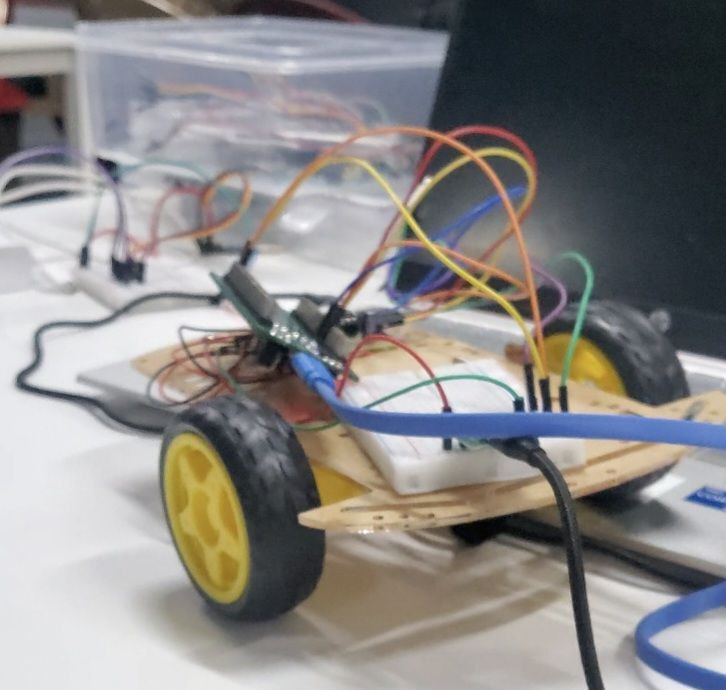
\includegraphics[width=0.3\columnwidth]{figs/8.jpg}
\caption{After all connections}
\end{figure}

\section{Code Execution For Bluetooth Toycar}
\raggedright

\item Now,Execute the following code
\begin{lstlisting}
vaman/toycar/codes/bluetooth_toycar/src
\end{lstlisting}

\item Build the ESP32 firmware
\begin{lstlisting}
cd  vaman/toycar/codes/bluetooth_toycar
pio run
\end{lstlisting} 

\item Flash ESP32 firmware ( connect Arduino-UART  )
\begin{lstlisting}
pio run -t upload
\end{lstlisting} 
\item Install the \textbf{Dabble app} on the Mobile from the \textbf{Playstore}. Connect it to the \textbf{ESP32} on the Vaman Board using \textbf{Bluetooth}. Change the controls to \textbf{Joystick mode} as shown in \figref{fig:ble_app}to navigate the UGV.\\

\section{Code Execution for Integrated Bluetooth Toycar}
\raggedright
\item Now,Execute the following code 

\begin{lstlisting}
vaman/toycar/codes/bluetooth_toycar
\end{lstlisting}

\item Build the ESP32 firmware
\begin{lstlisting}
cd esp32_pwmctrl
pio run
\end{lstlisting} 

\item Flash ESP32 firmware ( connect Arduino-UART  )
\begin{lstlisting}
pio run -t nobuild -t upload
\end{lstlisting} 

\item If using termux, send .pio/build/esp32doit-devkit-v1/firmware.bin to PC using
\begin{lstlisting}
scp .pio/build/esp32doit-devkit-v1/firmware.bin Username@IPAddress:
\end{lstlisting} 

\item  Modify line 140 of config.mk to setup path to pygmy-sdk and then Build m4 firmware using
\begin{lstlisting}
cd m4_pwmctrl/GCC_Project
make
\end{lstlisting}

\item If using termux, send output/m4{\_}pwmctrl.bin to PC using
\begin{lstlisting}
scp output/m4_pwmctrl.bin username@IPaddress:
\end{lstlisting} 

\item Build fpga source (.bin file)
\begin{lstlisting}
cd fpga_pwmctrl/rtl
ql_symbiflow -compile -d ql-eos-s3 -P pu64 -v *.v -t AL4S3B_FPGA_Top -p quickfeather.pcf -dump jlink binary 
\end{lstlisting} 

\item If using termux, send AL4S3B{\_}FPGA{\_}Top.bin to PC using
\begin{lstlisting}
scp AL4S3B_FPGA_Top.bin username@IPaddress:
\end{lstlisting} 

\item Connect usb cable to vaman board and Flash eos s3 soc, using
\begin{lstlisting}
sudo python3 <Type path to tiny fpga programmer application> --port /dev/ttyACM0  --appfpga AL4S3B_FPGA_Top.bin --m4app m4_pwmctrl.bin --mode m4-fpga --reset
\end{lstlisting} 

\item Install the \textbf{Dabble app} on the Mobile from the \textbf{Playstore}. Connect it to the \textbf{ESP32} on the Vaman Board using \textbf{Bluetooth}. Change the controls to \textbf{Joystick mode} as shown in \figref{fig:ble_app}to navigate the UGV.\\
\subsection{Working }
On the hardware level there are three key points: SPI,Wishbone Interfacing and Address Mapping. Vaman Board, we have an EOS S3 and ESP32. The Communication between these two happens via Serial Peripheral Interface(SPI).\\
\vspace{0.25cm}

\begin{figure}[!ht]
\centering
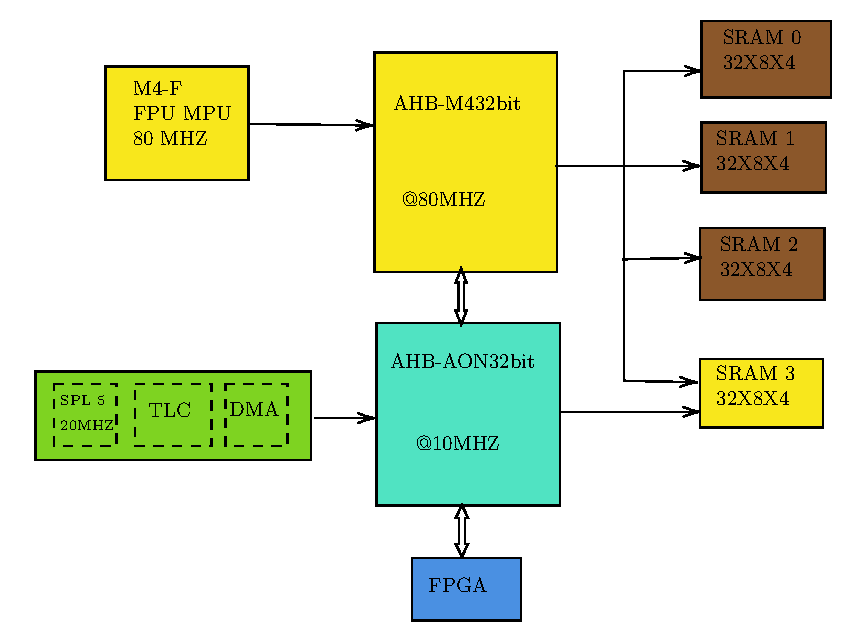
\includegraphics[width=0.5\columnwidth]{figs/block3}
\centering
\caption{EOS S3 Architecture }
\end{figure}

\begin{figure}[!ht]
\centering
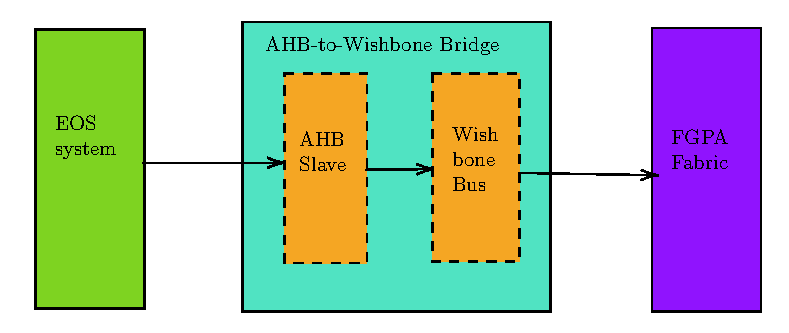
\includegraphics[width=0.5\columnwidth]{figs/block4}
\centering
\caption{Wishbone Slave Interface  }
\end{figure}
\begin{figure}[!ht]
\centering
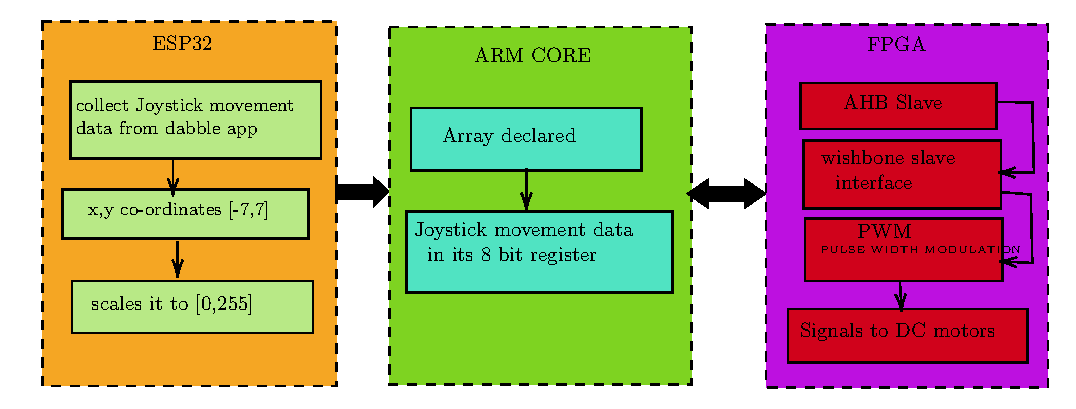
\includegraphics[width=0.5\columnwidth]{figs/block5}
\centering
\caption{Hardware Block level Architecture }
\end{figure}

\end{enumerate}
\chapter{Pulse Width Modulation}
This chapter demonstrates various applications of Pulse Width Modulation (PWM)
using the Vaman board.
\section{Onboard LED}
This section illustrates the use of SPI Communication between the Vaman-ESP32
and the Vaman-Pygmy in adjusting the brightness of an LED onboard the 
Vaman-Pygmy.

\subsection{Components}
The components required are listed in \autoref{tab:pwm-led-components}.
\begin{table}[!ht]
    \centering
    %%%%%%%%%%%%%%%%%%%%%%%%%%%%%%%%%%%%%%%%%%%%%%%%%%%%%%%%%%%%%%%%%%%%%%
%%                                                                  %%
%%  This is the header of a LaTeX2e file exported from Gnumeric.    %%
%%                                                                  %%
%%  This file can be compiled as it stands or included in another   %%
%%  LaTeX document. The table is based on the longtable package so  %%
%%  the longtable options (headers, footers...) can be set in the   %%
%%  preamble section below (see PRAMBLE).                           %%
%%                                                                  %%
%%  To include the file in another, the following two lines must be %%
%%  in the including file:                                          %%
%%        \def\inputGnumericTable{}                                 %%
%%  at the beginning of the file and:                               %%
%%        \input{name-of-this-file.tex}                             %%
%%  where the table is to be placed. Note also that the including   %%
%%  file must use the following packages for the table to be        %%
%%  rendered correctly:                                             %%
%%    \usepackage[latin1]{inputenc}                                 %%
%%    \usepackage{color}                                            %%
%%    \usepackage{array}                                            %%
%%    \usepackage{longtable}                                        %%
%%    \usepackage{calc}                                             %%
%%    \usepackage{multirow}                                         %%
%%    \usepackage{hhline}                                           %%
%%    \usepackage{ifthen}                                           %%
%%  optionally (for landscape tables embedded in another document): %%
%%    \usepackage{lscape}                                           %%
%%                                                                  %%
%%%%%%%%%%%%%%%%%%%%%%%%%%%%%%%%%%%%%%%%%%%%%%%%%%%%%%%%%%%%%%%%%%%%%%



%%  This section checks if we are begin input into another file or  %%
%%  the file will be compiled alone. First use a macro taken from   %%
%%  the TeXbook ex 7.7 (suggestion of Han-Wen Nienhuys).            %%
\def\ifundefined#1{\expandafter\ifx\csname#1\endcsname\relax}


%%  Check for the \def token for inputed files. If it is not        %%
%%  defined, the file will be processed as a standalone and the     %%
%%  preamble will be used.                                          %%
\ifundefined{inputGnumericTable}

%%  We must be able to close or not the document at the end.        %%
	\def\gnumericTableEnd{\end{document}}


%%%%%%%%%%%%%%%%%%%%%%%%%%%%%%%%%%%%%%%%%%%%%%%%%%%%%%%%%%%%%%%%%%%%%%
%%                                                                  %%
%%  This is the PREAMBLE. Change these values to get the right      %%
%%  paper size and other niceties.                                  %%
%%                                                                  %%
%%%%%%%%%%%%%%%%%%%%%%%%%%%%%%%%%%%%%%%%%%%%%%%%%%%%%%%%%%%%%%%%%%%%%%

	\documentclass[12pt%
			  %,landscape%
                    ]{report}
       \usepackage[latin1]{inputenc}
       \usepackage{fullpage}
       \usepackage{color}
       \usepackage{array}
       \usepackage{longtable}
       \usepackage{calc}
       \usepackage{multirow}
       \usepackage{hhline}
       \usepackage{ifthen}

	\begin{document}


%%  End of the preamble for the standalone. The next section is for %%
%%  documents which are included into other LaTeX2e files.          %%
\else

%%  We are not a stand alone document. For a regular table, we will %%
%%  have no preamble and only define the closing to mean nothing.   %%
    \def\gnumericTableEnd{}

%%  If we want landscape mode in an embedded document, comment out  %%
%%  the line above and uncomment the two below. The table will      %%
%%  begin on a new page and run in landscape mode.                  %%
%       \def\gnumericTableEnd{\end{landscape}}
%       \begin{landscape}


%%  End of the else clause for this file being \input.              %%
\fi

%%%%%%%%%%%%%%%%%%%%%%%%%%%%%%%%%%%%%%%%%%%%%%%%%%%%%%%%%%%%%%%%%%%%%%
%%                                                                  %%
%%  The rest is the gnumeric table, except for the closing          %%
%%  statement. Changes below will alter the table's appearance.     %%
%%                                                                  %%
%%%%%%%%%%%%%%%%%%%%%%%%%%%%%%%%%%%%%%%%%%%%%%%%%%%%%%%%%%%%%%%%%%%%%%

\providecommand{\gnumericmathit}[1]{#1} 
%%  Uncomment the next line if you would like your numbers to be in %%
%%  italics if they are italizised in the gnumeric table.           %%
%\renewcommand{\gnumericmathit}[1]{\mathit{#1}}
\providecommand{\gnumericPB}[1]%
{\let\gnumericTemp=\\#1\let\\=\gnumericTemp\hspace{0pt}}
 \ifundefined{gnumericTableWidthDefined}
        \newlength{\gnumericTableWidth}
        \newlength{\gnumericTableWidthComplete}
        \newlength{\gnumericMultiRowLength}
        \global\def\gnumericTableWidthDefined{}
 \fi
%% The following setting protects this code from babel shorthands.  %%
 \ifthenelse{\isundefined{\languageshorthands}}{}{\languageshorthands{english}}
%%  The default table format retains the relative column widths of  %%
%%  gnumeric. They can easily be changed to c, r or l. In that case %%
%%  you may want to comment out the next line and uncomment the one %%
%%  thereafter                                                      %%
\providecommand\gnumbox{\makebox[0pt]}
%%\providecommand\gnumbox[1][]{\makebox}

%% to adjust positions in multirow situations                       %%
\setlength{\bigstrutjot}{\jot}
\setlength{\extrarowheight}{\doublerulesep}

%%  The \setlongtables command keeps column widths the same across  %%
%%  pages. Simply comment out next line for varying column widths.  %%
\setlongtables

\setlength\gnumericTableWidth{%
	92pt+%
	104pt+%
	60pt+%
	70pt+%
0pt}
\def\gumericNumCols{4}
\setlength\gnumericTableWidthComplete{\gnumericTableWidth+%
         \tabcolsep*\gumericNumCols*2+\arrayrulewidth*\gumericNumCols}
\ifthenelse{\lengthtest{\gnumericTableWidthComplete > \linewidth}}%
         {\def\gnumericScale{1*\ratio{\linewidth-%
                        \tabcolsep*\gumericNumCols*2-%
                        \arrayrulewidth*\gumericNumCols}%
{\gnumericTableWidth}}}%
{\def\gnumericScale{1}}

%%%%%%%%%%%%%%%%%%%%%%%%%%%%%%%%%%%%%%%%%%%%%%%%%%%%%%%%%%%%%%%%%%%%%%
%%                                                                  %%
%% The following are the widths of the various columns. We are      %%
%% defining them here because then they are easier to change.       %%
%% Depending on the cell formats we may use them more than once.    %%
%%                                                                  %%
%%%%%%%%%%%%%%%%%%%%%%%%%%%%%%%%%%%%%%%%%%%%%%%%%%%%%%%%%%%%%%%%%%%%%%

\ifthenelse{\isundefined{\gnumericColA}}{\newlength{\gnumericColA}}{}\settowidth{\gnumericColA}{\begin{tabular}{@{}p{92pt*\gnumericScale}@{}}x\end{tabular}}
\ifthenelse{\isundefined{\gnumericColB}}{\newlength{\gnumericColB}}{}\settowidth{\gnumericColB}{\begin{tabular}{@{}p{104pt*\gnumericScale}@{}}x\end{tabular}}
\ifthenelse{\isundefined{\gnumericColC}}{\newlength{\gnumericColC}}{}\settowidth{\gnumericColC}{\begin{tabular}{@{}p{60pt*\gnumericScale}@{}}x\end{tabular}}
\ifthenelse{\isundefined{\gnumericColD}}{\newlength{\gnumericColD}}{}\settowidth{\gnumericColD}{\begin{tabular}{@{}p{70pt*\gnumericScale}@{}}x\end{tabular}}

\begin{tabular}[c]{%
	b{\gnumericColA}%
	b{\gnumericColB}%
	b{\gnumericColC}%
	b{\gnumericColD}%
	}

%%%%%%%%%%%%%%%%%%%%%%%%%%%%%%%%%%%%%%%%%%%%%%%%%%%%%%%%%%%%%%%%%%%%%%
%%  The longtable options. (Caption, headers... see Goosens, p.124) %%
%	\caption{The Table Caption.}             \\	%
% \hline	% Across the top of the table.
%%  The rest of these options are table rows which are placed on    %%
%%  the first, last or every page. Use \multicolumn if you want.    %%

%%  Header for the first page.                                      %%
%	\multicolumn{4}{c}{The First Header} \\ \hline 
%	\multicolumn{1}{c}{colTag}	%Column 1
%	&\multicolumn{1}{c}{colTag}	%Column 2
%	&\multicolumn{1}{c}{colTag}	%Column 3
%	&\multicolumn{1}{c}{colTag}	\\ \hline %Last column
%	\endfirsthead

%%  The running header definition.                                  %%
%	\hline
%	\multicolumn{4}{l}{\ldots\small\slshape continued} \\ \hline
%	\multicolumn{1}{c}{colTag}	%Column 1
%	&\multicolumn{1}{c}{colTag}	%Column 2
%	&\multicolumn{1}{c}{colTag}	%Column 3
%	&\multicolumn{1}{c}{colTag}	\\ \hline %Last column
%	\endhead

%%  The running footer definition.                                  %%
%	\hline
%	\multicolumn{4}{r}{\small\slshape continued\ldots} \\
%	\endfoot

%%  The ending footer definition.                                   %%
%	\multicolumn{4}{c}{That's all folks} \\ \hline 
%	\endlastfoot
%%%%%%%%%%%%%%%%%%%%%%%%%%%%%%%%%%%%%%%%%%%%%%%%%%%%%%%%%%%%%%%%%%%%%%

\hhline{|-|-|-~}
	 \multicolumn{1}{|p{\gnumericColA}|}%
	{\gnumericPB{\centering}\gnumbox{\textbf{Component}}}
	&\multicolumn{1}{p{\gnumericColB}|}%
	{\gnumericPB{\centering}\gnumbox{\textbf{Value}}}
	&\multicolumn{1}{p{\gnumericColC}|}%
	{\gnumericPB{\centering}\gnumbox{\textbf{Quantity}}}
	&
\\
\hhline{|---|~}
	 \multicolumn{1}{|p{\gnumericColA}|}%
	{\gnumericPB{\centering}\gnumbox{Vaman}}
	&\multicolumn{1}{p{\gnumericColB}|}%
	{\gnumericPB{\centering}\gnumbox{LC}}
	&\multicolumn{1}{p{\gnumericColC}|}%
	{\gnumericPB{\centering}\gnumbox{1}}
	&
\\
\hhline{|---|~}
	 \multicolumn{1}{|p{\gnumericColA}|}%
	{\gnumericPB{\centering}\gnumbox{Jumper Wires}}
	&\multicolumn{1}{p{\gnumericColB}|}%
	{\gnumericPB{\centering}\gnumbox{Female-to-Female}}
	&\multicolumn{1}{p{\gnumericColC}|}%
	{\gnumericPB{\centering}\gnumbox{20}}
	&
\\
\hhline{|---|~}
	 \multicolumn{1}{|p{\gnumericColA}|}%
	{\gnumericPB{\centering}\gnumbox{USB-UART}}
	&\multicolumn{1}{p{\gnumericColB}|}%
	{}
	&\multicolumn{1}{p{\gnumericColC}|}%
	{\gnumericPB{\centering}\gnumbox{1}}
	&
\\
\hhline{|---|~}
	 \multicolumn{1}{|p{\gnumericColA}|}%
	{\gnumericPB{\centering}\gnumbox{USB Cable}}
	&\multicolumn{1}{p{\gnumericColB}|}%
	{\gnumericPB{\centering}\gnumbox{Type-B}}
	&\multicolumn{1}{p{\gnumericColC}|}%
	{\gnumericPB{\centering}\gnumbox{1}}
	&
\\
\hhline{|-|-|-|~}
\end{tabular}

\ifthenelse{\isundefined{\languageshorthands}}{}{\languageshorthands{\languagename}}
\gnumericTableEnd

    \caption{Components Required for Controlling the Onboard LED via SPI.}
    \label{tab:pwm-led-components}
\end{table}

\subsection{Connections}
The connections on the Vaman board are listed in
\autoref{tab:pwm-led-connections}.
\begin{table}[!ht]
    \centering
    %%%%%%%%%%%%%%%%%%%%%%%%%%%%%%%%%%%%%%%%%%%%%%%%%%%%%%%%%%%%%%%%%%%%%%
%%                                                                  %%
%%  This is the header of a LaTeX2e file exported from Gnumeric.    %%
%%                                                                  %%
%%  This file can be compiled as it stands or included in another   %%
%%  LaTeX document. The table is based on the longtable package so  %%
%%  the longtable options (headers, footers...) can be set in the   %%
%%  preamble section below (see PRAMBLE).                           %%
%%                                                                  %%
%%  To include the file in another, the following two lines must be %%
%%  in the including file:                                          %%
%%        \def\inputGnumericTable{}                                 %%
%%  at the beginning of the file and:                               %%
%%        \input{name-of-this-file.tex}                             %%
%%  where the table is to be placed. Note also that the including   %%
%%  file must use the following packages for the table to be        %%
%%  rendered correctly:                                             %%
%%    \usepackage[latin1]{inputenc}                                 %%
%%    \usepackage{color}                                            %%
%%    \usepackage{array}                                            %%
%%    \usepackage{longtable}                                        %%
%%    \usepackage{calc}                                             %%
%%    \usepackage{multirow}                                         %%
%%    \usepackage{hhline}                                           %%
%%    \usepackage{ifthen}                                           %%
%%  optionally (for landscape tables embedded in another document): %%
%%    \usepackage{lscape}                                           %%
%%                                                                  %%
%%%%%%%%%%%%%%%%%%%%%%%%%%%%%%%%%%%%%%%%%%%%%%%%%%%%%%%%%%%%%%%%%%%%%%



%%  This section checks if we are begin input into another file or  %%
%%  the file will be compiled alone. First use a macro taken from   %%
%%  the TeXbook ex 7.7 (suggestion of Han-Wen Nienhuys).            %%
\def\ifundefined#1{\expandafter\ifx\csname#1\endcsname\relax}


%%  Check for the \def token for inputed files. If it is not        %%
%%  defined, the file will be processed as a standalone and the     %%
%%  preamble will be used.                                          %%
\ifundefined{inputGnumericTable}

%%  We must be able to close or not the document at the end.        %%
	\def\gnumericTableEnd{\end{document}}


%%%%%%%%%%%%%%%%%%%%%%%%%%%%%%%%%%%%%%%%%%%%%%%%%%%%%%%%%%%%%%%%%%%%%%
%%                                                                  %%
%%  This is the PREAMBLE. Change these values to get the right      %%
%%  paper size and other niceties.                                  %%
%%                                                                  %%
%%%%%%%%%%%%%%%%%%%%%%%%%%%%%%%%%%%%%%%%%%%%%%%%%%%%%%%%%%%%%%%%%%%%%%

	\documentclass[12pt%
			  %,landscape%
                    ]{report}
       \usepackage[latin1]{inputenc}
       \usepackage{fullpage}
       \usepackage{color}
       \usepackage{array}
       \usepackage{longtable}
       \usepackage{calc}
       \usepackage{multirow}
       \usepackage{hhline}
       \usepackage{ifthen}

	\begin{document}


%%  End of the preamble for the standalone. The next section is for %%
%%  documents which are included into other LaTeX2e files.          %%
\else

%%  We are not a stand alone document. For a regular table, we will %%
%%  have no preamble and only define the closing to mean nothing.   %%
    \def\gnumericTableEnd{}

%%  If we want landscape mode in an embedded document, comment out  %%
%%  the line above and uncomment the two below. The table will      %%
%%  begin on a new page and run in landscape mode.                  %%
%       \def\gnumericTableEnd{\end{landscape}}
%       \begin{landscape}


%%  End of the else clause for this file being \input.              %%
\fi

%%%%%%%%%%%%%%%%%%%%%%%%%%%%%%%%%%%%%%%%%%%%%%%%%%%%%%%%%%%%%%%%%%%%%%
%%                                                                  %%
%%  The rest is the gnumeric table, except for the closing          %%
%%  statement. Changes below will alter the table's appearance.     %%
%%                                                                  %%
%%%%%%%%%%%%%%%%%%%%%%%%%%%%%%%%%%%%%%%%%%%%%%%%%%%%%%%%%%%%%%%%%%%%%%

\providecommand{\gnumericmathit}[1]{#1} 
%%  Uncomment the next line if you would like your numbers to be in %%
%%  italics if they are italizised in the gnumeric table.           %%
%\renewcommand{\gnumericmathit}[1]{\mathit{#1}}
\providecommand{\gnumericPB}[1]%
{\let\gnumericTemp=\\#1\let\\=\gnumericTemp\hspace{0pt}}
 \ifundefined{gnumericTableWidthDefined}
        \newlength{\gnumericTableWidth}
        \newlength{\gnumericTableWidthComplete}
        \newlength{\gnumericMultiRowLength}
        \global\def\gnumericTableWidthDefined{}
 \fi
%% The following setting protects this code from babel shorthands.  %%
 \ifthenelse{\isundefined{\languageshorthands}}{}{\languageshorthands{english}}
%%  The default table format retains the relative column widths of  %%
%%  gnumeric. They can easily be changed to c, r or l. In that case %%
%%  you may want to comment out the next line and uncomment the one %%
%%  thereafter                                                      %%
\providecommand\gnumbox{\makebox[0pt]}
%%\providecommand\gnumbox[1][]{\makebox}

%% to adjust positions in multirow situations                       %%
\setlength{\bigstrutjot}{\jot}
\setlength{\extrarowheight}{\doublerulesep}

%%  The \setlongtables command keeps column widths the same across  %%
%%  pages. Simply comment out next line for varying column widths.  %%
\setlongtables

\setlength\gnumericTableWidth{%
	66pt+%
	95pt+%
	80pt+%
	70pt+%
0pt}
\def\gumericNumCols{4}
\setlength\gnumericTableWidthComplete{\gnumericTableWidth+%
         \tabcolsep*\gumericNumCols*2+\arrayrulewidth*\gumericNumCols}
\ifthenelse{\lengthtest{\gnumericTableWidthComplete > \linewidth}}%
         {\def\gnumericScale{1*\ratio{\linewidth-%
                        \tabcolsep*\gumericNumCols*2-%
                        \arrayrulewidth*\gumericNumCols}%
{\gnumericTableWidth}}}%
{\def\gnumericScale{1}}

%%%%%%%%%%%%%%%%%%%%%%%%%%%%%%%%%%%%%%%%%%%%%%%%%%%%%%%%%%%%%%%%%%%%%%
%%                                                                  %%
%% The following are the widths of the various columns. We are      %%
%% defining them here because then they are easier to change.       %%
%% Depending on the cell formats we may use them more than once.    %%
%%                                                                  %%
%%%%%%%%%%%%%%%%%%%%%%%%%%%%%%%%%%%%%%%%%%%%%%%%%%%%%%%%%%%%%%%%%%%%%%

\ifthenelse{\isundefined{\gnumericColA}}{\newlength{\gnumericColA}}{}\settowidth{\gnumericColA}{\begin{tabular}{@{}p{66pt*\gnumericScale}@{}}x\end{tabular}}
\ifthenelse{\isundefined{\gnumericColB}}{\newlength{\gnumericColB}}{}\settowidth{\gnumericColB}{\begin{tabular}{@{}p{95pt*\gnumericScale}@{}}x\end{tabular}}
\ifthenelse{\isundefined{\gnumericColC}}{\newlength{\gnumericColC}}{}\settowidth{\gnumericColC}{\begin{tabular}{@{}p{80pt*\gnumericScale}@{}}x\end{tabular}}
\ifthenelse{\isundefined{\gnumericColD}}{\newlength{\gnumericColD}}{}\settowidth{\gnumericColD}{\begin{tabular}{@{}p{70pt*\gnumericScale}@{}}x\end{tabular}}

\begin{tabular}[c]{%
	b{\gnumericColA}%
	b{\gnumericColB}%
	b{\gnumericColC}%
	b{\gnumericColD}%
	}

%%%%%%%%%%%%%%%%%%%%%%%%%%%%%%%%%%%%%%%%%%%%%%%%%%%%%%%%%%%%%%%%%%%%%%
%%  The longtable options. (Caption, headers... see Goosens, p.124) %%
%	\caption{The Table Caption.}             \\	%
% \hline	% Across the top of the table.
%%  The rest of these options are table rows which are placed on    %%
%%  the first, last or every page. Use \multicolumn if you want.    %%

%%  Header for the first page.                                      %%
%	\multicolumn{4}{c}{The First Header} \\ \hline 
%	\multicolumn{1}{c}{colTag}	%Column 1
%	&\multicolumn{1}{c}{colTag}	%Column 2
%	&\multicolumn{1}{c}{colTag}	%Column 3
%	&\multicolumn{1}{c}{colTag}	\\ \hline %Last column
%	\endfirsthead

%%  The running header definition.                                  %%
%	\hline
%	\multicolumn{4}{l}{\ldots\small\slshape continued} \\ \hline
%	\multicolumn{1}{c}{colTag}	%Column 1
%	&\multicolumn{1}{c}{colTag}	%Column 2
%	&\multicolumn{1}{c}{colTag}	%Column 3
%	&\multicolumn{1}{c}{colTag}	\\ \hline %Last column
%	\endhead

%%  The running footer definition.                                  %%
%	\hline
%	\multicolumn{4}{r}{\small\slshape continued\ldots} \\
%	\endfoot

%%  The ending footer definition.                                   %%
%	\multicolumn{4}{c}{That's all folks} \\ \hline 
%	\endlastfoot
%%%%%%%%%%%%%%%%%%%%%%%%%%%%%%%%%%%%%%%%%%%%%%%%%%%%%%%%%%%%%%%%%%%%%%

\hhline{|-|-|-~}
	 \multicolumn{1}{|p{\gnumericColA}|}%
	{\gnumericPB{\centering}\gnumbox{\textbf{Pin}}}
	&\multicolumn{1}{p{\gnumericColB}|}%
	{\gnumericPB{\centering}\gnumbox{\textbf{Vaman-ESP32}}}
	&\multicolumn{1}{p{\gnumericColC}|}%
	{\gnumericPB{\centering}\gnumbox{\textbf{Vaman-Pygmy}}}
	&
\\
\hhline{|---|~}
	 \multicolumn{1}{|p{\gnumericColA}|}%
	{\gnumericPB{\centering}\gnumbox{CS/SS}}
	&\multicolumn{1}{p{\gnumericColB}|}%
	{\gnumericPB{\centering}\gnumbox{27}}
	&\multicolumn{1}{p{\gnumericColC}|}%
	{\gnumericPB{\centering}\gnumbox{20}}
	&
\\
\hhline{|---|~}
	 \multicolumn{1}{|p{\gnumericColA}|}%
	{\gnumericPB{\centering}\gnumbox{CIPO/MISO}}
	&\multicolumn{1}{p{\gnumericColB}|}%
	{\gnumericPB{\centering}\gnumbox{19}}
	&\multicolumn{1}{p{\gnumericColC}|}%
	{\gnumericPB{\centering}\gnumbox{17}}
	&
\\
\hhline{|---|~}
	 \multicolumn{1}{|p{\gnumericColA}|}%
	{\gnumericPB{\centering}\gnumbox{COPI/MOSI}}
	&\multicolumn{1}{p{\gnumericColB}|}%
	{\gnumericPB{\centering}\gnumbox{18}}
	&\multicolumn{1}{p{\gnumericColC}|}%
	{\gnumericPB{\centering}\gnumbox{19}}
	&
\\
\hhline{|---|~}
	 \multicolumn{1}{|p{\gnumericColA}|}%
	{\gnumericPB{\centering}\gnumbox{SCLK}}
	&\multicolumn{1}{p{\gnumericColB}|}%
	{\gnumericPB{\centering}\gnumbox{5}}
	&\multicolumn{1}{p{\gnumericColC}|}%
	{\gnumericPB{\centering}\gnumbox{16}}
	&
\\
\hhline{|-|-|-|~}
\end{tabular}

\ifthenelse{\isundefined{\languageshorthands}}{}{\languageshorthands{\languagename}}
\gnumericTableEnd

    \caption{Connections to establish SPI between Vaman-ESP32 and Vaman-Pygmy.}
    \label{tab:pwm-led-connections}
\end{table}

\subsection{Building}
\begin{enumerate}
    \item Build the PlatformIO project at
    \begin{lstlisting}
pwm/led/codes/esp32
    \end{lstlisting}
    \item Flash the project .bin file using USB-UART connected to the 
    Vaman-ESP32, via PlatformIO or ArduinoDroid.
    \item Build the FPGA project .bin file by entering the following commands at
    a terminal window.
    \begin{lstlisting}
# The following variable can be sourced from .shellrc or .venv/bin/activate
export QORC_SDK_PATH=/path/to/pygmy-sdk
cd pwm/led/codes/fpga
make
    \end{lstlisting}
    \item On building successfully, the file
    \begin{lstlisting}
pwm/led/codes/fpga/rtl/AL4S3B_FPGA_Top.bin
    \end{lstlisting}
    is generated.
    \item Edit the variable PROJ\_ROOT in
    \begin{lstlisting}
pwm/led/codes/m4/GCC_Project/config.mk
    \end{lstlisting}
    to point to the location of the pygmy-sdk folder on your system.
    \item Build the M4 project .bin file by entering the following commands at a
    terminal window.
    \begin{lstlisting}
cd pwm/led/codes/m4/GCC_Project
make -j4
    \end{lstlisting}
    \item Flash both FPGA and M4 .bin files to the Vaman-Pygmy by resetting it
    to bootloader mode and entering the following command at a terminal window.
    \begin{lstlisting}
python3 /path/to/tinyfpga-programmer-gui.py --port /dev/ttyACMxx --mode m4-fpga --m4app /path/to/m4.bin --appfpga /path/to/AL4S3B_FPGA_Top.bin --reset
    \end{lstlisting}
    where /dev/ttyACMxx is the port at which the Vaman board is available. This
    can be obtained by inspecting the output of the following command (requires
    root/sudo privileges).
    \begin{lstlisting}
dmesg -w
    \end{lstlisting}
\end{enumerate}

\subsection{Demonstration}
\begin{enumerate}[resume]
    \item Find the IP address of the Vaman-ESP32 by inspecting the output of the
    serial terminal, or by typing at a terminal window
    \begin{lstlisting}
ifconfig
nmap -sn xx.yy.zz.0/24
    \end{lstlisting}
    where xx.yy.zz represents the first three octets of the IP address of your
    device on the WiFi network interface, found using \texttt{ifconfig}.
    \item Then, go to the site 
    \begin{lstlisting}
http://<VAMAN-IP>/pwm 
    \end{lstlisting}
    and enter the PWM value, which is an integer between 0 and 255.
    \item On entering the value, the brightness of the green LED will change 
    according to the PWM value.
\end{enumerate}

\subsection{Exercises}
\begin{enumerate}[resume]
    \item Add code to gradually increase or decrease brightness of the onboard
    LED.
    \item Avoid using the M4 platform entirely by having the ESP32 write to the
    appropriate memory address of the PWM using SPI directly.
\end{enumerate}
\section{UGV}
This section illustrates the use of SPI Communication between the Vaman-ESP32
and the Vaman-Pygmy in adjusting the speed of the UGV.

\subsection{Components}
\begin{table}[!ht]
    \centering
    %%%%%%%%%%%%%%%%%%%%%%%%%%%%%%%%%%%%%%%%%%%%%%%%%%%%%%%%%%%%%%%%%%%%%%
%%                                                                  %%
%%  This is the header of a LaTeX2e file exported from Gnumeric.    %%
%%                                                                  %%
%%  This file can be compiled as it stands or included in another   %%
%%  LaTeX document. The table is based on the longtable package so  %%
%%  the longtable options (headers, footers...) can be set in the   %%
%%  preamble section below (see PRAMBLE).                           %%
%%                                                                  %%
%%  To include the file in another, the following two lines must be %%
%%  in the including file:                                          %%
%%        \def\inputGnumericTable{}                                 %%
%%  at the beginning of the file and:                               %%
%%        \input{name-of-this-file.tex}                             %%
%%  where the table is to be placed. Note also that the including   %%
%%  file must use the following packages for the table to be        %%
%%  rendered correctly:                                             %%
%%    \usepackage[latin1]{inputenc}                                 %%
%%    \usepackage{color}                                            %%
%%    \usepackage{array}                                            %%
%%    \usepackage{longtable}                                        %%
%%    \usepackage{calc}                                             %%
%%    \usepackage{multirow}                                         %%
%%    \usepackage{hhline}                                           %%
%%    \usepackage{ifthen}                                           %%
%%  optionally (for landscape tables embedded in another document): %%
%%    \usepackage{lscape}                                           %%
%%                                                                  %%
%%%%%%%%%%%%%%%%%%%%%%%%%%%%%%%%%%%%%%%%%%%%%%%%%%%%%%%%%%%%%%%%%%%%%%



%%  This section checks if we are begin input into another file or  %%
%%  the file will be compiled alone. First use a macro taken from   %%
%%  the TeXbook ex 7.7 (suggestion of Han-Wen Nienhuys).            %%
\def\ifundefined#1{\expandafter\ifx\csname#1\endcsname\relax}


%%  Check for the \def token for inputed files. If it is not        %%
%%  defined, the file will be processed as a standalone and the     %%
%%  preamble will be used.                                          %%
\ifundefined{inputGnumericTable}

%%  We must be able to close or not the document at the end.        %%
	\def\gnumericTableEnd{\end{document}}


%%%%%%%%%%%%%%%%%%%%%%%%%%%%%%%%%%%%%%%%%%%%%%%%%%%%%%%%%%%%%%%%%%%%%%
%%                                                                  %%
%%  This is the PREAMBLE. Change these values to get the right      %%
%%  paper size and other niceties.                                  %%
%%                                                                  %%
%%%%%%%%%%%%%%%%%%%%%%%%%%%%%%%%%%%%%%%%%%%%%%%%%%%%%%%%%%%%%%%%%%%%%%

	\documentclass[12pt%
			  %,landscape%
                    ]{report}
       \usepackage[latin1]{inputenc}
       \usepackage{fullpage}
       \usepackage{color}
       \usepackage{array}
       \usepackage{longtable}
       \usepackage{calc}
       \usepackage{multirow}
       \usepackage{hhline}
       \usepackage{ifthen}

	\begin{document}


%%  End of the preamble for the standalone. The next section is for %%
%%  documents which are included into other LaTeX2e files.          %%
\else

%%  We are not a stand alone document. For a regular table, we will %%
%%  have no preamble and only define the closing to mean nothing.   %%
    \def\gnumericTableEnd{}

%%  If we want landscape mode in an embedded document, comment out  %%
%%  the line above and uncomment the two below. The table will      %%
%%  begin on a new page and run in landscape mode.                  %%
%       \def\gnumericTableEnd{\end{landscape}}
%       \begin{landscape}


%%  End of the else clause for this file being \input.              %%
\fi

%%%%%%%%%%%%%%%%%%%%%%%%%%%%%%%%%%%%%%%%%%%%%%%%%%%%%%%%%%%%%%%%%%%%%%
%%                                                                  %%
%%  The rest is the gnumeric table, except for the closing          %%
%%  statement. Changes below will alter the table's appearance.     %%
%%                                                                  %%
%%%%%%%%%%%%%%%%%%%%%%%%%%%%%%%%%%%%%%%%%%%%%%%%%%%%%%%%%%%%%%%%%%%%%%

\providecommand{\gnumericmathit}[1]{#1} 
%%  Uncomment the next line if you would like your numbers to be in %%
%%  italics if they are italizised in the gnumeric table.           %%
%\renewcommand{\gnumericmathit}[1]{\mathit{#1}}
\providecommand{\gnumericPB}[1]%
{\let\gnumericTemp=\\#1\let\\=\gnumericTemp\hspace{0pt}}
 \ifundefined{gnumericTableWidthDefined}
        \newlength{\gnumericTableWidth}
        \newlength{\gnumericTableWidthComplete}
        \newlength{\gnumericMultiRowLength}
        \global\def\gnumericTableWidthDefined{}
 \fi
%% The following setting protects this code from babel shorthands.  %%
 \ifthenelse{\isundefined{\languageshorthands}}{}{\languageshorthands{english}}
%%  The default table format retains the relative column widths of  %%
%%  gnumeric. They can easily be changed to c, r or l. In that case %%
%%  you may want to comment out the next line and uncomment the one %%
%%  thereafter                                                      %%
\providecommand\gnumbox{\makebox[0pt]}
%%\providecommand\gnumbox[1][]{\makebox}

%% to adjust positions in multirow situations                       %%
\setlength{\bigstrutjot}{\jot}
\setlength{\extrarowheight}{\doublerulesep}

%%  The \setlongtables command keeps column widths the same across  %%
%%  pages. Simply comment out next line for varying column widths.  %%
\setlongtables

\setlength\gnumericTableWidth{%
	121pt+%
	96pt+%
	70pt+%
0pt}
\def\gumericNumCols{3}
\setlength\gnumericTableWidthComplete{\gnumericTableWidth+%
         \tabcolsep*\gumericNumCols*2+\arrayrulewidth*\gumericNumCols}
\ifthenelse{\lengthtest{\gnumericTableWidthComplete > \linewidth}}%
         {\def\gnumericScale{1*\ratio{\linewidth-%
                        \tabcolsep*\gumericNumCols*2-%
                        \arrayrulewidth*\gumericNumCols}%
{\gnumericTableWidth}}}%
{\def\gnumericScale{1}}

%%%%%%%%%%%%%%%%%%%%%%%%%%%%%%%%%%%%%%%%%%%%%%%%%%%%%%%%%%%%%%%%%%%%%%
%%                                                                  %%
%% The following are the widths of the various columns. We are      %%
%% defining them here because then they are easier to change.       %%
%% Depending on the cell formats we may use them more than once.    %%
%%                                                                  %%
%%%%%%%%%%%%%%%%%%%%%%%%%%%%%%%%%%%%%%%%%%%%%%%%%%%%%%%%%%%%%%%%%%%%%%

\ifthenelse{\isundefined{\gnumericColA}}{\newlength{\gnumericColA}}{}\settowidth{\gnumericColA}{\begin{tabular}{@{}p{121pt*\gnumericScale}@{}}x\end{tabular}}
\ifthenelse{\isundefined{\gnumericColB}}{\newlength{\gnumericColB}}{}\settowidth{\gnumericColB}{\begin{tabular}{@{}p{96pt*\gnumericScale}@{}}x\end{tabular}}
\ifthenelse{\isundefined{\gnumericColC}}{\newlength{\gnumericColC}}{}\settowidth{\gnumericColC}{\begin{tabular}{@{}p{70pt*\gnumericScale}@{}}x\end{tabular}}

\begin{tabular}[c]{%
	b{\gnumericColA}%
	b{\gnumericColB}%
	b{\gnumericColC}%
	}

%%%%%%%%%%%%%%%%%%%%%%%%%%%%%%%%%%%%%%%%%%%%%%%%%%%%%%%%%%%%%%%%%%%%%%
%%  The longtable options. (Caption, headers... see Goosens, p.124) %%
%	\caption{The Table Caption.}             \\	%
% \hline	% Across the top of the table.
%%  The rest of these options are table rows which are placed on    %%
%%  the first, last or every page. Use \multicolumn if you want.    %%

%%  Header for the first page.                                      %%
%	\multicolumn{3}{c}{The First Header} \\ \hline 
%	\multicolumn{1}{c}{colTag}	%Column 1
%	&\multicolumn{1}{c}{colTag}	%Column 2
%	&\multicolumn{1}{c}{colTag}	\\ \hline %Last column
%	\endfirsthead

%%  The running header definition.                                  %%
%	\hline
%	\multicolumn{3}{l}{\ldots\small\slshape continued} \\ \hline
%	\multicolumn{1}{c}{colTag}	%Column 1
%	&\multicolumn{1}{c}{colTag}	%Column 2
%	&\multicolumn{1}{c}{colTag}	\\ \hline %Last column
%	\endhead

%%  The running footer definition.                                  %%
%	\hline
%	\multicolumn{3}{r}{\small\slshape continued\ldots} \\
%	\endfoot

%%  The ending footer definition.                                   %%
%	\multicolumn{3}{c}{That's all folks} \\ \hline 
%	\endlastfoot
%%%%%%%%%%%%%%%%%%%%%%%%%%%%%%%%%%%%%%%%%%%%%%%%%%%%%%%%%%%%%%%%%%%%%%

\hhline{|-|-|-}
	 \multicolumn{1}{|p{\gnumericColA}|}%
	{\gnumericPB{\centering}\gnumbox{\textbf{Component}}}
	&\multicolumn{1}{p{\gnumericColB}|}%
	{\gnumericPB{\centering}\gnumbox{\textbf{Value}}}
	&\multicolumn{1}{p{\gnumericColC}|}%
	{\gnumericPB{\centering}\gnumbox{\textbf{Quantity}}}
\\
\hhline{|---|}
	 \multicolumn{1}{|p{\gnumericColA}|}%
	{\gnumericPB{\centering}\gnumbox{Vaman}}
	&\multicolumn{1}{p{\gnumericColB}|}%
	{\gnumericPB{\centering}\gnumbox{LC}}
	&\multicolumn{1}{p{\gnumericColC}|}%
	{\gnumericPB{\centering}\gnumbox{1}}
\\
\hhline{|---|}
	 \multicolumn{1}{|p{\gnumericColA}|}%
	{\gnumericPB{\centering}\gnumbox{USB-UART}}
	&\multicolumn{1}{p{\gnumericColB}|}%
	{}
	&\multicolumn{1}{p{\gnumericColC}|}%
	{\gnumericPB{\centering}\gnumbox{1}}
\\
\hhline{|---|}
	 \multicolumn{1}{|p{\gnumericColA}|}%
	{\gnumericPB{\centering}\gnumbox{Jumper Wires}}
	&\multicolumn{1}{p{\gnumericColB}|}%
	{\gnumericPB{\centering}\gnumbox{Male-to-Female}}
	&\multicolumn{1}{p{\gnumericColC}|}%
	{\gnumericPB{\centering}\gnumbox{20}}
\\
\hhline{|---|}
	 \multicolumn{1}{|p{\gnumericColA}|}%
	{\gnumericPB{\centering}\gnumbox{USB Cable}}
	&\multicolumn{1}{p{\gnumericColB}|}%
	{\gnumericPB{\centering}\gnumbox{Type-B}}
	&\multicolumn{1}{p{\gnumericColC}|}%
	{\gnumericPB{\centering}\gnumbox{1}}
\\
\hhline{|---|}
	 \multicolumn{1}{|p{\gnumericColA}|}%
	{\gnumericPB{\centering}\gnumbox{Breadboard}}
	&\multicolumn{1}{p{\gnumericColB}|}%
	{}
	&\multicolumn{1}{p{\gnumericColC}|}%
	{\gnumericPB{\centering}\gnumbox{1}}
\\
\hhline{|---|}
	 \multicolumn{1}{|p{\gnumericColA}|}%
	{\gnumericPB{\centering}\gnumbox{Battery}}
	&\multicolumn{1}{p{\gnumericColB}|}%
	{\gnumericPB{\centering}\gnumbox{12 V}}
	&\multicolumn{1}{p{\gnumericColC}|}%
	{\gnumericPB{\centering}\gnumbox{1}}
\\
\hhline{|---|}
	 \multicolumn{1}{|p{\gnumericColA}|}%
	{\gnumericPB{\centering}\gnumbox{UGV Kit}}
	&\multicolumn{1}{p{\gnumericColB}|}%
	{}
	&\multicolumn{1}{p{\gnumericColC}|}%
	{\gnumericPB{\centering}\gnumbox{1}}
\\
\hhline{|-|-|-|}
\end{tabular}

\ifthenelse{\isundefined{\languageshorthands}}{}{\languageshorthands{\languagename}}
\gnumericTableEnd

    \caption{Components Required for Controlling the UGV PWM via SPI.}
    \label{tab:pwm-ugv-components}
\end{table}

\subsection{Connections}
\begin{table}[!ht]
    \centering
    %%%%%%%%%%%%%%%%%%%%%%%%%%%%%%%%%%%%%%%%%%%%%%%%%%%%%%%%%%%%%%%%%%%%%%
%%                                                                  %%
%%  This is the header of a LaTeX2e file exported from Gnumeric.    %%
%%                                                                  %%
%%  This file can be compiled as it stands or included in another   %%
%%  LaTeX document. The table is based on the longtable package so  %%
%%  the longtable options (headers, footers...) can be set in the   %%
%%  preamble section below (see PRAMBLE).                           %%
%%                                                                  %%
%%  To include the file in another, the following two lines must be %%
%%  in the including file:                                          %%
%%        \def\inputGnumericTable{}                                 %%
%%  at the beginning of the file and:                               %%
%%        \input{name-of-this-file.tex}                             %%
%%  where the table is to be placed. Note also that the including   %%
%%  file must use the following packages for the table to be        %%
%%  rendered correctly:                                             %%
%%    \usepackage[latin1]{inputenc}                                 %%
%%    \usepackage{color}                                            %%
%%    \usepackage{array}                                            %%
%%    \usepackage{longtable}                                        %%
%%    \usepackage{calc}                                             %%
%%    \usepackage{multirow}                                         %%
%%    \usepackage{hhline}                                           %%
%%    \usepackage{ifthen}                                           %%
%%  optionally (for landscape tables embedded in another document): %%
%%    \usepackage{lscape}                                           %%
%%                                                                  %%
%%%%%%%%%%%%%%%%%%%%%%%%%%%%%%%%%%%%%%%%%%%%%%%%%%%%%%%%%%%%%%%%%%%%%%



%%  This section checks if we are begin input into another file or  %%
%%  the file will be compiled alone. First use a macro taken from   %%
%%  the TeXbook ex 7.7 (suggestion of Han-Wen Nienhuys).            %%
\def\ifundefined#1{\expandafter\ifx\csname#1\endcsname\relax}


%%  Check for the \def token for inputed files. If it is not        %%
%%  defined, the file will be processed as a standalone and the     %%
%%  preamble will be used.                                          %%
\ifundefined{inputGnumericTable}

%%  We must be able to close or not the document at the end.        %%
	\def\gnumericTableEnd{\end{document}}


%%%%%%%%%%%%%%%%%%%%%%%%%%%%%%%%%%%%%%%%%%%%%%%%%%%%%%%%%%%%%%%%%%%%%%
%%                                                                  %%
%%  This is the PREAMBLE. Change these values to get the right      %%
%%  paper size and other niceties.                                  %%
%%                                                                  %%
%%%%%%%%%%%%%%%%%%%%%%%%%%%%%%%%%%%%%%%%%%%%%%%%%%%%%%%%%%%%%%%%%%%%%%

	\documentclass[12pt%
			  %,landscape%
                    ]{report}
       \usepackage[latin1]{inputenc}
       \usepackage{fullpage}
       \usepackage{color}
       \usepackage{array}
       \usepackage{longtable}
       \usepackage{calc}
       \usepackage{multirow}
       \usepackage{hhline}
       \usepackage{ifthen}

	\begin{document}


%%  End of the preamble for the standalone. The next section is for %%
%%  documents which are included into other LaTeX2e files.          %%
\else

%%  We are not a stand alone document. For a regular table, we will %%
%%  have no preamble and only define the closing to mean nothing.   %%
    \def\gnumericTableEnd{}

%%  If we want landscape mode in an embedded document, comment out  %%
%%  the line above and uncomment the two below. The table will      %%
%%  begin on a new page and run in landscape mode.                  %%
%       \def\gnumericTableEnd{\end{landscape}}
%       \begin{landscape}


%%  End of the else clause for this file being \input.              %%
\fi

%%%%%%%%%%%%%%%%%%%%%%%%%%%%%%%%%%%%%%%%%%%%%%%%%%%%%%%%%%%%%%%%%%%%%%
%%                                                                  %%
%%  The rest is the gnumeric table, except for the closing          %%
%%  statement. Changes below will alter the table's appearance.     %%
%%                                                                  %%
%%%%%%%%%%%%%%%%%%%%%%%%%%%%%%%%%%%%%%%%%%%%%%%%%%%%%%%%%%%%%%%%%%%%%%

\providecommand{\gnumericmathit}[1]{#1} 
%%  Uncomment the next line if you would like your numbers to be in %%
%%  italics if they are italizised in the gnumeric table.           %%
%\renewcommand{\gnumericmathit}[1]{\mathit{#1}}
\providecommand{\gnumericPB}[1]%
{\let\gnumericTemp=\\#1\let\\=\gnumericTemp\hspace{0pt}}
 \ifundefined{gnumericTableWidthDefined}
        \newlength{\gnumericTableWidth}
        \newlength{\gnumericTableWidthComplete}
        \newlength{\gnumericMultiRowLength}
        \global\def\gnumericTableWidthDefined{}
 \fi
%% The following setting protects this code from babel shorthands.  %%
 \ifthenelse{\isundefined{\languageshorthands}}{}{\languageshorthands{english}}
%%  The default table format retains the relative column widths of  %%
%%  gnumeric. They can easily be changed to c, r or l. In that case %%
%%  you may want to comment out the next line and uncomment the one %%
%%  thereafter                                                      %%
\providecommand\gnumbox{\makebox[0pt]}
%%\providecommand\gnumbox[1][]{\makebox}

%% to adjust positions in multirow situations                       %%
\setlength{\bigstrutjot}{\jot}
\setlength{\extrarowheight}{\doublerulesep}

%%  The \setlongtables command keeps column widths the same across  %%
%%  pages. Simply comment out next line for varying column widths.  %%
\setlongtables

\setlength\gnumericTableWidth{%
	65pt+%
	85pt+%
	75pt+%
	70pt+%
0pt}
\def\gumericNumCols{4}
\setlength\gnumericTableWidthComplete{\gnumericTableWidth+%
         \tabcolsep*\gumericNumCols*2+\arrayrulewidth*\gumericNumCols}
\ifthenelse{\lengthtest{\gnumericTableWidthComplete > \linewidth}}%
         {\def\gnumericScale{1*\ratio{\linewidth-%
                        \tabcolsep*\gumericNumCols*2-%
                        \arrayrulewidth*\gumericNumCols}%
{\gnumericTableWidth}}}%
{\def\gnumericScale{1}}

%%%%%%%%%%%%%%%%%%%%%%%%%%%%%%%%%%%%%%%%%%%%%%%%%%%%%%%%%%%%%%%%%%%%%%
%%                                                                  %%
%% The following are the widths of the various columns. We are      %%
%% defining them here because then they are easier to change.       %%
%% Depending on the cell formats we may use them more than once.    %%
%%                                                                  %%
%%%%%%%%%%%%%%%%%%%%%%%%%%%%%%%%%%%%%%%%%%%%%%%%%%%%%%%%%%%%%%%%%%%%%%

\ifthenelse{\isundefined{\gnumericColA}}{\newlength{\gnumericColA}}{}\settowidth{\gnumericColA}{\begin{tabular}{@{}p{65pt*\gnumericScale}@{}}x\end{tabular}}
\ifthenelse{\isundefined{\gnumericColB}}{\newlength{\gnumericColB}}{}\settowidth{\gnumericColB}{\begin{tabular}{@{}p{85pt*\gnumericScale}@{}}x\end{tabular}}
\ifthenelse{\isundefined{\gnumericColC}}{\newlength{\gnumericColC}}{}\settowidth{\gnumericColC}{\begin{tabular}{@{}p{75pt*\gnumericScale}@{}}x\end{tabular}}
\ifthenelse{\isundefined{\gnumericColD}}{\newlength{\gnumericColD}}{}\settowidth{\gnumericColD}{\begin{tabular}{@{}p{70pt*\gnumericScale}@{}}x\end{tabular}}

\begin{tabular}[c]{%
	b{\gnumericColA}%
	b{\gnumericColB}%
	b{\gnumericColC}%
	b{\gnumericColD}%
	}

%%%%%%%%%%%%%%%%%%%%%%%%%%%%%%%%%%%%%%%%%%%%%%%%%%%%%%%%%%%%%%%%%%%%%%
%%  The longtable options. (Caption, headers... see Goosens, p.124) %%
%	\caption{The Table Caption.}             \\	%
% \hline	% Across the top of the table.
%%  The rest of these options are table rows which are placed on    %%
%%  the first, last or every page. Use \multicolumn if you want.    %%

%%  Header for the first page.                                      %%
%	\multicolumn{4}{c}{The First Header} \\ \hline 
%	\multicolumn{1}{c}{colTag}	%Column 1
%	&\multicolumn{1}{c}{colTag}	%Column 2
%	&\multicolumn{1}{c}{colTag}	%Column 3
%	&\multicolumn{1}{c}{colTag}	\\ \hline %Last column
%	\endfirsthead

%%  The running header definition.                                  %%
%	\hline
%	\multicolumn{4}{l}{\ldots\small\slshape continued} \\ \hline
%	\multicolumn{1}{c}{colTag}	%Column 1
%	&\multicolumn{1}{c}{colTag}	%Column 2
%	&\multicolumn{1}{c}{colTag}	%Column 3
%	&\multicolumn{1}{c}{colTag}	\\ \hline %Last column
%	\endhead

%%  The running footer definition.                                  %%
%	\hline
%	\multicolumn{4}{r}{\small\slshape continued\ldots} \\
%	\endfoot

%%  The ending footer definition.                                   %%
%	\multicolumn{4}{c}{That's all folks} \\ \hline 
%	\endlastfoot
%%%%%%%%%%%%%%%%%%%%%%%%%%%%%%%%%%%%%%%%%%%%%%%%%%%%%%%%%%%%%%%%%%%%%%

\hhline{|-|-|-~}
	 \multicolumn{1}{|p{\gnumericColA}|}%
	{\gnumericPB{\centering}\gnumbox{\textbf{L293 IC}}}
	&\multicolumn{1}{p{\gnumericColB}|}%
	{\gnumericPB{\centering}\gnumbox{\textbf{Vaman-Pygmy}}}
	&\multicolumn{1}{p{\gnumericColC}|}%
	{\gnumericPB{\centering}\gnumbox{\textbf{12 V Battery}}}
	&
\\
\hhline{|---|~}
	 \multicolumn{1}{|p{\gnumericColA}|}%
	{\gnumericPB{\centering}\gnumbox{MA1}}
	&\multicolumn{1}{p{\gnumericColB}|}%
	{\setlength{\gnumericMultiRowLength}{0pt}%
	 \addtolength{\gnumericMultiRowLength}{\gnumericColB}%
	 \multirow{2}[1]{\gnumericMultiRowLength}{\parbox{\gnumericMultiRowLength}{%
	 \gnumericPB{\centering}\gnumbox{IO\_18}}}}
	&\multicolumn{1}{p{\gnumericColC}|}%
	{}
	&
\\
\hhline{|-|~|-|~}
	 \multicolumn{1}{|p{\gnumericColA}|}%
	{\gnumericPB{\centering}\gnumbox{MA2}}
	&\multicolumn{1}{p{\gnumericColB}|}%
	{}
	&\multicolumn{1}{p{\gnumericColC}|}%
	{}
	&
\\
\hhline{|---|~}
	 \multicolumn{1}{|p{\gnumericColA}|}%
	{\gnumericPB{\centering}\gnumbox{MB1}}
	&\multicolumn{1}{p{\gnumericColB}|}%
	{\setlength{\gnumericMultiRowLength}{0pt}%
	 \addtolength{\gnumericMultiRowLength}{\gnumericColB}%
	 \multirow{2}[1]{\gnumericMultiRowLength}{\parbox{\gnumericMultiRowLength}{%
	 \gnumericPB{\centering}\gnumbox{IO\_22}}}}
	&\multicolumn{1}{p{\gnumericColC}|}%
	{}
	&
\\
\hhline{|-|~|-|~}
	 \multicolumn{1}{|p{\gnumericColA}|}%
	{\gnumericPB{\centering}\gnumbox{MB2}}
	&\multicolumn{1}{p{\gnumericColB}|}%
	{}
	&\multicolumn{1}{p{\gnumericColC}|}%
	{}
	&
\\
\hhline{|---|~}
	 \multicolumn{1}{|p{\gnumericColA}|}%
	{\gnumericPB{\centering}\gnumbox{ENA}}
	&\multicolumn{1}{p{\gnumericColB}|}%
	{\setlength{\gnumericMultiRowLength}{0pt}%
	 \addtolength{\gnumericMultiRowLength}{\gnumericColB}%
	 \multirow{2}[1]{\gnumericMultiRowLength}{\parbox{\gnumericMultiRowLength}{%
	 \gnumericPB{\centering}\gnumbox{3v3}}}}
	&\multicolumn{1}{p{\gnumericColC}|}%
	{}
	&
\\
\hhline{|-|~|-|~}
	 \multicolumn{1}{|p{\gnumericColA}|}%
	{\gnumericPB{\centering}\gnumbox{ENB}}
	&\multicolumn{1}{p{\gnumericColB}|}%
	{}
	&\multicolumn{1}{p{\gnumericColC}|}%
	{}
	&
\\
\hhline{|---|~}
	 \multicolumn{1}{|p{\gnumericColA}|}%
	{\gnumericPB{\centering}\gnumbox{VCC}}
	&\multicolumn{1}{p{\gnumericColB}|}%
	{}
	&\multicolumn{1}{p{\gnumericColC}|}%
	{\gnumericPB{\centering}\gnumbox{12 V}}
	&
\\
\hhline{|---|~}
	 \multicolumn{1}{|p{\gnumericColA}|}%
	{\gnumericPB{\centering}\gnumbox{GND}}
	&\multicolumn{1}{p{\gnumericColB}|}%
	{}
	&\multicolumn{1}{p{\gnumericColC}|}%
	{\gnumericPB{\centering}\gnumbox{GND}}
	&
\\
\hhline{|-|-|-|~}
\end{tabular}

\ifthenelse{\isundefined{\languageshorthands}}{}{\languageshorthands{\languagename}}
\gnumericTableEnd

    \caption{Connections to establish SPI between Vaman-ESP32 and Vaman-Pygmy.}
    \label{tab:pwm-ugv-connections}
\end{table}

\subsection{Building}
\begin{enumerate}
    \item Build the PlatformIO project at
    \begin{lstlisting}
pwm/ugv/codes/esp32
    \end{lstlisting}
    \item Flash the project .bin file using USB-UART connected to the 
    Vaman-ESP32, via PlatformIO or ArduinoDroid.
    \item Build the FPGA project .bin file by entering the following commands at
    a terminal window.
    \begin{lstlisting}
# The following variable can be sourced from .shellrc or .venv/bin/activate
export QORC_SDK_PATH=/path/to/pygmy-sdk
cd pwm/ugv/codes/fpga
make
    \end{lstlisting}
    \item On building successfully, the file
    \begin{lstlisting}
pwm/ugv/codes/fpga/rtl/AL4S3B_FPGA_Top.bin
    \end{lstlisting}
    is generated.
    \item Edit the variable PROJ\_ROOT in
    \begin{lstlisting}
pwm/ugv/codes/m4/GCC_Project/config.mk
    \end{lstlisting}
    to point to the location of the pygmy-sdk folder on your system.
    \item Build the M4 project .bin file by entering the following commands at a
    terminal window.
    \begin{lstlisting}
cd pwm/ugv/codes/m4/GCC_Project
make -j4
    \end{lstlisting}
    \item Flash both FPGA and M4 .bin files to the Vaman-Pygmy by resetting it
    to bootloader mode and entering the following command at a terminal window.
    \begin{lstlisting}
python3 /path/to/tinyfpga-programmer-gui.py --port /dev/ttyACMxx --mode m4-fpga --m4app /path/to/m4.bin --appfpga /path/to/AL4S3B_FPGA_Top.bin --reset
    \end{lstlisting}
    where /dev/ttyACMxx is the port at which the Vaman board is available. This
    can be obtained by inspecting the output of the following command (requires
    root/sudo privileges).
    \begin{lstlisting}
dmesg -w
    \end{lstlisting}
\end{enumerate}

\subsection{Demonstration}
\begin{enumerate}[resume]
    \item Find the IP address of the Vaman-ESP32 by inspecting the output of the
    serial terminal, or by typing at a terminal window
    \begin{lstlisting}
ifconfig
nmap -sn xx.yy.zz.0/24
    \end{lstlisting}
    where xx.yy.zz represents the first three octets of the IP address of your
    device on the WiFi network interface, found using \texttt{ifconfig}.
    \item Then, go to the site 
    \begin{lstlisting}
http://<VAMAN-IP>/pwm 
    \end{lstlisting}
    and enter the PWM value, which is an integer between 0 and 255.
    \item On entering the value, the speed of the UGV will change according to
    the PWM value.
\end{enumerate}
\backmatter
\appendix
\iffalse
\chapter{Manual}
\input{manual/gvv_opt.tex}
\fi
\latexprintindex

\end{document}